% 
% Licensed to the Apache Software Foundation (ASF) under one
% or more contributor license agreements.  See the NOTICE file
% distributed with this work for additional information
% regarding copyright ownership.  The ASF licenses this file
% to you under the Apache License, Version 2.0 (the
% "License"); you may not use this file except in compliance
% with the License.  You may obtain a copy of the License at
% 
%   http://www.apache.org/licenses/LICENSE-2.0
% 
% Unless required by applicable law or agreed to in writing,
% software distributed under the License is distributed on an
% "AS IS" BASIS, WITHOUT WARRANTIES OR CONDITIONS OF ANY
% KIND, either express or implied.  See the License for the
% specific language governing permissions and limitations
% under the License.
% 
\documentclass[oneside]{book}

% space between paragraphs
\usepackage{parskip}

% import graphics
%\usepackage[pdftex]{graphicx}
\usepackage{graphicx}

% Better control of figure placement
\usepackage{float}

% hyperlinks
\usepackage[colorlinks,linkcolor=blue]{hyperref}

% Conditionally execute based on PDF or HTML output
\usepackage{ifpdf}

% Margins
\usepackage[top=1in, bottom=.75in, left=.75in, right=.75in ]{geometry}

\usepackage{xcolor}

\usepackage{caption} 
\captionsetup[table]{skip=18pt}

%list margins
\usepackage{enumitem}

% better control over date formatting
\usepackage{datetime}

\title{\Huge \textbf{Distributed UIMA Cluster Computing}}
\author{Written and maintained by the Apache\\
UIMA\texttrademark Development Community \\
\\
\\
\\
Version 1.0.0}

\date{}

\begin{document}

\frontmatter
\maketitle


%Licensed to the Apache Software Foundation (ASF) under one
%or more contributor license agreements.  See the NOTICE file
%distributed with this work for additional information
%regarding copyright ownership.  The ASF licenses this file
%to you under the Apache License, Version 2.0 (the
%"License"); you may not use this file except in compliance
%with the License.  You may obtain a copy of the License at
%
%   http://www.apache.org/licenses/LICENSE-2.0
%
%Unless required by applicable law or agreed to in writing,
%software distributed under the License is distributed on an
%"AS IS" BASIS, WITHOUT WARRANTIES OR CONDITIONS OF ANY
%KIND, either express or implied.  See the License for the
%specific language governing permissions and limitations
%under the License.
Copyright \copyright~ 2012 The Apache Software Foundation

Copyright \copyright~ 2012 International Business Machines Corporation

{\addtolength{\leftskip}{10 mm}
     \paragraph{License and Disclaimer}
     The ASF licenses this documentation to you under the Apache License, Version 2.0 (the "License");
     you may not use this documentation except in compliance with the License.  You may obtain a copy of
     the License at
              
     \url{http://www.apache.org/licenses/LICENSE-2.0}
     
     Unless required by applicable law or agreed to in writing, this documentation and its contents are
     distributed under the License on an "AS IS" BASIS, WITHOUT WARRANTIES OR CONDITIONS OF ANY KIND,
     either express or implied.  See the License for the specific language governing permissions and
     limitations under the License.

     \paragraph{Trademarks}     
     All terms mentioned in the text that are known to be trademarks or service marks have been
     appropriately capitalized.  Use of such terms in this book should not be regarded as affecting the
     validity of the the trademark or service mark.

}

\vspace{.5in}

\newdateformat{mydate}{%
\monthname~\THEYEAR}

Publication date: \mydate\today


%% \setcounter{tocdepth}{4}
% Call it Table Of Contents, same as other UIMA books do
\renewcommand\contentsname{Table of Contents}
\tableofcontents
\listoffigures
% \listoftables

\mainmatter

% 
% Licensed to the Apache Software Foundation (ASF) under one
% or more contributor license agreements.  See the NOTICE file
% distributed with this work for additional information
% regarding copyright ownership.  The ASF licenses this file
% to you under the Apache License, Version 2.0 (the
% "License"); you may not use this file except in compliance
% with the License.  You may obtain a copy of the License at
% 
%   http://www.apache.org/licenses/LICENSE-2.0
% 
% Unless required by applicable law or agreed to in writing,
% software distributed under the License is distributed on an
% "AS IS" BASIS, WITHOUT WARRANTIES OR CONDITIONS OF ANY
% KIND, either express or implied.  See the License for the
% specific language governing permissions and limitations
% under the License.
% 
% common macros in a single place
% These are used in the main file, and in the stand-alone wrappers
\newcommand{\distro}{apache-uima-ducc-1.0.0.tgz}
\newcommand{\duccruntime}{DUCC\_HOME}
\newcommand{\ducchome}{DUCC\_HOME}
\newcommand{\todo}{{\sc \Large TODO:}  }
\newcommand{\note}{{\em Note:}  }
\newcommand{\cfbox}[2]{%
    \colorlet{currentcolor}{.}%
    {\color{#1}%
    \fbox{\color{currentcolor}#2}}%
}


\part{DUCC Concepts}
% 
% Licensed to the Apache Software Foundation (ASF) under one
% or more contributor license agreements.  See the NOTICE file
% distributed with this work for additional information
% regarding copyright ownership.  The ASF licenses this file
% to you under the Apache License, Version 2.0 (the
% "License"); you may not use this file except in compliance
% with the License.  You may obtain a copy of the License at
% 
%   http://www.apache.org/licenses/LICENSE-2.0
% 
% Unless required by applicable law or agreed to in writing,
% software distributed under the License is distributed on an
% "AS IS" BASIS, WITHOUT WARRANTIES OR CONDITIONS OF ANY
% KIND, either express or implied.  See the License for the
% specific language governing permissions and limitations
% under the License.
% 
% Create well-known link to this spot for HTML version
\ifpdf
\else
\HCode{<a name='DUCC_OVERVIEW'></a>}
\fi
\chapter{DUCC Overview}

    \section{What is DUCC?}

    DUCC stands for Distributed UIMA Cluster Computing. DUCC is a cluster management system
    providing tooling, management, and scheduling facilities to automate the scale-out of
    applications written to the UIMA framework.

    Core UIMA provides a generalized framework for applications that process unstructured
    information such as human language, but does not provide a scale-out mechanism. UIMA-AS provides
    a scale-out mechanism to distribute UIMA pipelines over a cluster of computing resources, but
    does not provide job or cluster management of the resources. DUCC defines a formal job model
    that closely maps to a standard UIMA pipeline. Around this job model DUCC provides cluster
    management services to automate the scale-out of UIMA pipelines over computing clusters.

    \section{DUCC Job Model}

    The Job Model defines the steps necessary to scale-up a UIMA pipeline using DUCC.  The goal of
    DUCC is to allow the application logic to be unchanged.

    The DUCC Job model consists of standard UIMA components: a Collection Reader (CR), a CAS
    Multiplier (CM), application logic as implemented one or more Analysis Engines (AE), and a CAS
    Consumer (CC).  In theory, any CR, or CM will work with DUCC, but DUCC is all about scale-out.  In
    order to achieve good scale-out these components must be constructed in a specific way.

    The Collection Reader builds input CASs and forwards them to the UIMA pipelines.  In the DUCC
    model, the CR is run in a process separate from the rest of the pipeline. In fact, in all but the
    smallest clusters it is run on a different physical machine than the rest of the pipeline.  To
    achieve scalability, the CR must create very small CASs that do not contain application data,
    but which contain references to data; for instance, file names.  Ideally, the CR should be
    runnable in a process not much larger than the smallest Java virtual machine.  Later sections
    demonstrate methods for achieving this.

    Each pipeline must contain at least one CAS Multiplier which receives the CASs from the CR.  The
    CMs encapsulate the knowledge of how to receive the data references in the small CASs received
    from the CRs and deliver the referenced data to the application pipeline.  DUCC packages the CM,
    AE(s), and CC into a single process, multiple instances of which are then deployed over the
    cluster.

    DUCC does not provide any mechanism for receiving output CASs.  Each application must
    supply its own CAS Consumer which serializes the output of the pipelines for 
    consumption by other entities (as serialized CASs, for example).

    A DUCC job therefore consists of a small specification containing the following items:
    
    \begin{itemize}
      \item The name of a resource containing the CR descriptor.
      \item The name of a resource containing the CM descriptor.
      \item The name of a resource containing the AE descriptor.
      \item The name of a resource containing the CC descriptor.
      \item Other information required to parametrize the above and identify the job
        such as log directory, working directory, desired scale-out, etc.  These are
        described in detail in subsequent sections.
    \end{itemize}

    On job submission, DUCC examines the job specification and automatically creates a scaled-out
    UIMA-AS service with a single process executing the CR as a UIMA-AS client and and as many
    processes as possible executing the combined CM, AE, and CC pipeline as UIMA-AS service
    instances.

    DUCC provides other facilities in support of scale-out:
    \begin{itemize}
      \item The ability to reserve all or part of a node in the cluster.
      \item Automated management of services required in support of jobs.
      \item The ability to schedule and execute arbitrary processes on nodes in the
        cluster.
      \item Debugging tools and support.
      \item A web server to display and manage work and cluster status.
      \item A CLI and a Java API to support the above.
    \end{itemize}
    
    \section{DUCC From UIMA to Full Scale-out}

    In this section we demonstrate the progression of a simple UIMA pipeline to a fully
    scaled-out job running under DUCC.

    \paragraph{UIMA Pipelines}
    A normal UIMA pipeline
    contains a Collection Reader, one or more Analysis Engines connected in a pipeline, and a CAS
    Consumer as shown in \hyperref[fig:UIMA-pipeline]{Figure ~\ref{fig:UIMA-pipeline}}.

    \begin{figure}[H]
      \centering
%      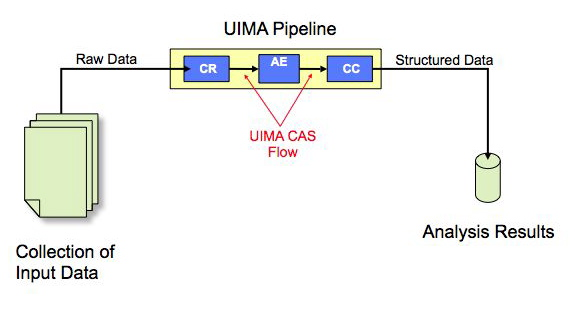
\includegraphics[bb=0 0 575 310, width=5.5in]{images/uima-pipeline.jpg}
      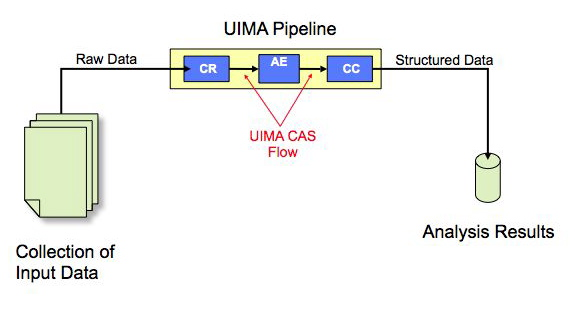
\includegraphics[width=5.5in]{images/uima-pipeline.jpg}
      \caption{Standard UIMA Pipeline}
      \label{fig:UIMA-pipeline}
    \end{figure}

    \paragraph{UIMA-AS  Scaled Pipeline}
    With UIMA-AS the CR is separated into a discrete process and a CAS Multiplier is introduced 
    into the pipeline as an interface between the CR and the pipeline, as shown in
    \hyperref[fig:UIMA-AS-pipeline]{Figure ~\ref{fig:UIMA-AS-pipeline}} below.
    Multiple pipelines are serviced by the 
    CR and are scaled-out over a computing cluster.  The difficulty with this model is that each
    user is individually responsible for finding and scheduling computing nodes, installing
    communication software such as ActiveMQ, and generally managing the distributed job and
    associated hardware.

    \begin{figure}[H]
      \centering
%      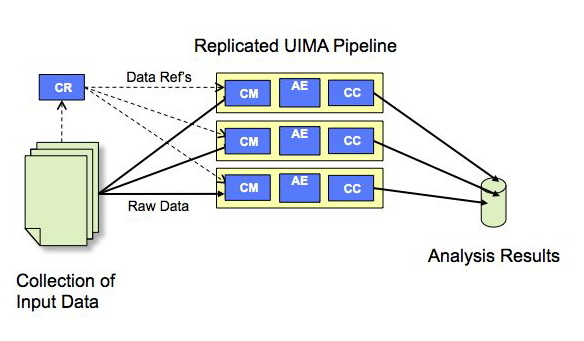
\includegraphics[bb=0 0 584 341, width=5.5in]{images/uima-as-pipeline.jpg}
      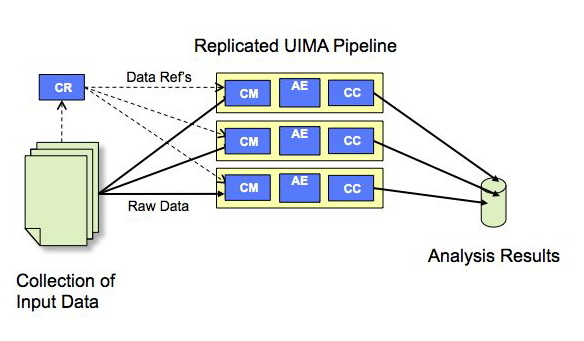
\includegraphics[width=5.5in]{images/uima-as-pipeline.jpg}
      \caption{UIMA Pipeline As Scaled by UIMA-AS}
      \label{fig:UIMA-AS-pipeline}
    \end{figure}

    \paragraph{UIMA-AS Pipeline Scaled By DUCC}
    DUCC is a UIMA and  UIMA-AS-aware cluster manager.  To scale out work under DUCC the developer
    tells DUCC what the parts of the application are, and DUCC does the work to build the
    scale-out via UIMA/AS, to find and schedule resources, to deploy the parts of the application
    over the cluster, and to manage the jobs while it executes.

    On job submission, the DUCC Command Line Interface (CLI) inspects the XML defining the analytic
    and generates a UIMA-AS Deployment Descriptor (DD).  The DD establishes some number of pipeline
    threads per process (as indicated in the DUCC job parameters), and generates job-unique queues.

    Under DUCC, the Collection Reader is executed in a process called the Job Driver (or JD). The 
    pipelines are executed in one or more processes called Job Processes (or JPs). The JD 
    process provides a thin wrapper over the CR to enable communication with DUCC.  The JD uses the
    CR to implement a UIMA-AS client delivering CASs to the multiple (scaled-out) pipelines, 
    shown in \hyperref[fig:UIMA-AS-pipeline-DUCC]{Figure ~\ref{fig:UIMA-AS-pipeline-DUCC}} below.

    \begin{figure}[H]
      \centering
%      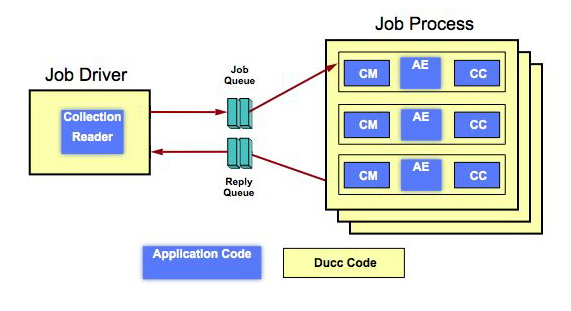
\includegraphics[bb=0 0 571 311, width=5.5in]{images/ducc-sequential.jpg}
      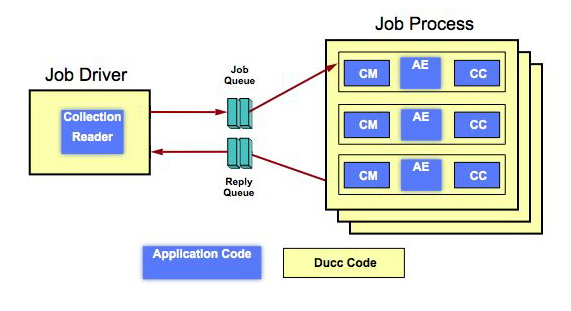
\includegraphics[width=5.5in]{images/ducc-sequential.jpg}
      \caption{UIMA Pipeline As Automatically Scaled Out By DUCC}
      \label{fig:UIMA-AS-pipeline-DUCC}
    \end{figure}

    \paragraph{UIMA-AS Pipeline with User-Supplied DD Scaled By DUCC}

    Application programmers may supply their own Deployment Descriptors to control intra-process
    threading and scale-out.  If a DD is supplied in the job parameters, DUCC will use this instead
    of generating one as depicted in \hyperref[fig:UIMA-AS-pipeline-DUCC-DD]{Figure ~\ref{fig:UIMA-AS-pipeline-DUCC-DD}} below.

    \begin{figure}[H]
      \centering
%      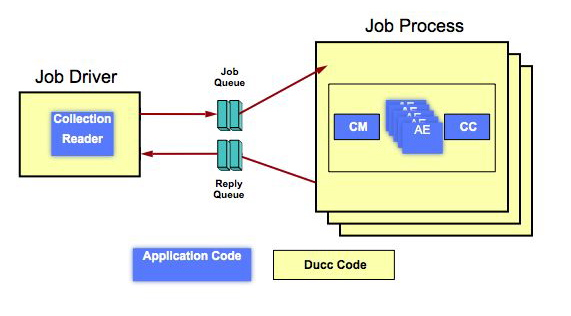
\includegraphics[bb=0 0 571 316,width=5.5in]{images/ducc-parallel.jpg}
      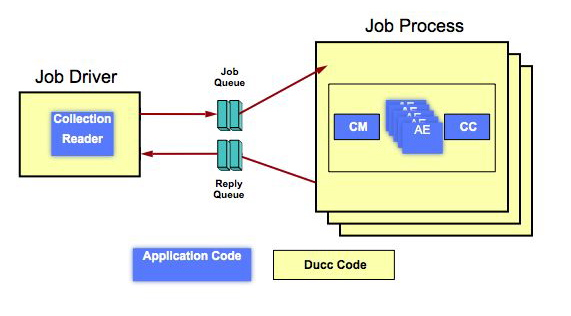
\includegraphics[width=5.5in]{images/ducc-parallel.jpg}
      \caption{UIMA Pipeline With User-Supplied DD as Automatically Scaled Out By DUCC}
      \label{fig:UIMA-AS-pipeline-DUCC-DD}
    \end{figure}

  
    \section{Error Management }
    DUCC provides a number of facilities to assist error management:
    
    \begin{itemize}
      \item DUCC uses the UIMA-AS error-handling facilities to reflect errors from the Job Processes
        to the Job Drivers. The JD wrappers implement logic to enforce error thresholds, to identify
        and log errors, and to reflect job problems in the DUCC Web Server.  All error thresholds are
        configurable both globally and on a per-job basis.

      \item Error and timeout thresholds are implemented for both the initialization phase of a pipeline
        and the execution phase.
    
      \item Retry-after-error is supported: if a process has a failure on some CAS after
        initialization is successful, the process is terminated and all affected CASs are retried, up to some
        configurable threshold.

      \item DUCC ensures that processes can successfully initialize before fully scaling out a job,
        to ensure a cluster is not overwhelmed with errant processes.

      \item Various error conditions encountered  while a job is running will prevent the errant job
        from continuing scale out, and can result in termination of the job.
      \end{itemize}
      
    \section{Cluster and Job Management}
    DUCC supports  management of multiple jobs and multiple users in a distributed cluster:

    \begin{description}
        \item[Multiple User Support] When properly configured, 
          DUCC runs all work under the identity of the submitting user. Logs
          are written with the user's credentials into the user's file space designated at job
          submission.

        \item[Fair-Share Scheduling] DUCC provides a Fair-Share scheduler to equitably share
          resources among multiple users.  The scheduler also supports semi-permanent reservation of
          full or partial machines.

        \item[Service Management] DUCC provides a Service Manager capable of automatically starting, stopping, and
          otherwise managing and querying both UIMA-AS and non-UIMA-AS services in support of jobs.

        \item[Job Lifetime Management and Orchestration] DUCC includes an Orchestrator to manage the
          lifetimes of all entities in the system.

        \item[Node Sharing] DUCC allocates processes from one or more users on a node, each with a specified
          amount of memory.  DUCC's preferred mechanism for constraining memory use is Linux
          Control Groups, or CGroups.  For nodes that do not suport CGroups, DUCC agents monitor
          RAM use and kill processes that exceed their share size by a settable fudge factor.

        \item[DUCC Agents] DUCC Agents manage each node's local resources and all
          processes started by DUCC. Each node in a cluster has exactly one Agent. The Agent
          \begin{itemize}
            \item Monitors and reports node capabilities (memory, etc) and performance data (CPU busy,
              swap, etc).
            \item Starts, stops, and monitors all processes on behalf of users.
            \item Patrols the node for ``foreign'' (non-DUCC) processes, reporting them to the
              Web Server, and optionally reaping them.
            \item Ensures job processes do not exceed their declared memory requirements
              through the use of Linux Cgroups.
          \end{itemize}

        \item[DUCC Web server] DUCC  provides a web server displaying all aspects of the system:
          \begin{itemize}
              \item All jobs in the system, their current state, resource usage, etc.
                
              \item All reserved resources and associated information (owner, etc.),
                including the ability to request and cancel reservations.
                
              \item All services, including the ability to start, stop, and modify
                service definitions.
                
              \item All nodes in the system and their status, usage, etc. 
                                
              \item The status of all DUCC management processes.  

              \item Access to documentation.
          \end{itemize}


        \item[Cluster Management Support] DUCC provides system management support to:
          \begin{itemize}
              \item Start, stop, and query full DUCC systems.
 
              \item Start, stop, and quiesce individual DUCC components.
 
              \item Add and delete nodes from the DUCC system.
 
              \item Discover DUCC processes (e.g. after partial failures).
 
              \item Find and kill errant job processes belonging to individual users.
                
              \item Monitor and display inter-DUCC messages.
          \end{itemize}
      \end{description}

    
    \section{Security Measures}
    The following DUCC security measures are provided:

    \begin{description}
    \item[user credentials] DUCC instantiates user processes using a setuid root executable named ducc\_ling.
    See more at \hyperref[sec:duccling.security]{\em ducc\_ling}.
    \item[command line interface] The CLI employs HTTP to send requests
    to the DUCC controller.  The CLI creates and employs public and private
    security keys in the user's home directory for authentication of HTTP
    requests.  The controller validates requests via these same security keys.
    \item[webserver] The webserver facilitates operational control and
    therefore authentication is desirable. 
    \begin{itemize}
    \item[\textit{user}] Each user has the ability to control certain aspects of
    only his/her active submissions.
    \item[\textit{admin}] Each administrator has the ability to control certain
    aspects of any user's active submissions, as well as modification of some
    DUCC operational characteristics.
    \end{itemize}
    A simple interface is provided so
    that an installation can plug-in a site specific authentication mechanism
    comprising userid and password.
    \item[ActiveMQ] DUCC uses ActiveMQ for administrative communication.
    AMQ authentication is used to prevent arbitrary processes from participating.
    \end{description}
    
    \subsection{ducc\_ling}   
    \label{sec:duccling.security}
           ducc\_ling contains the following functions, which the security-conscious may verify by examining
       the source in \duccruntime/duccling.  All sensitive operations are performed only AFTER switching
       userids, to prevent unauthorized root access to the system.
       \begin{itemize}
         \item Changes it's real and effective userid to that of the user invoking the job.
         \item Optionally redirects its stdout and stderr to the DUCC log for the current job.
         \item Optionally redirects its stdio to a port set by the CLI, when a job is submitted.
         \item ``Nice''s itself to a ``worse'' priority than the default, to reduce the chances
           that a runaway DUCC job could monopolize a system.
         \item Optionally sets user limits.
         \item Prints the effective limits for a job to both the user's log, and the DUCC agent's log.
         \item Changes to the user's working directory, as specified by the job.
         \item Optionally establishes LD\_LIBRARY\_PATH 
           for the job from the environment variable  {\tt DUCC\_LD\_LIBRARY\_PATH}
           if set in the DUCC job specification. (Secure Linux systems will
           prevent LD\_LIBRARY\_PATH 
           from being set by a program with root authority, so this is
           done AFTER changing userids).
         \item  ONLY user {\em ducc} may use the ducc\_ling program in
           a privileged way. Ducc\_ling contains checks to prevent even user {\em root} from using it for
           privileged operations. 

       \end{itemize}
    
    
    \section{Security Issues}
    The following DUCC security issues should be considered:
    
    \begin{description}
    \item[submit transmission 'sniffed'] In the event that the DUCC submit
    command is 'sniffed' then the user authentication mechanism is compromised
    and user masquerading is possible.  That is, the userid encryption mechanism
    can be exploited such that user A can submit a job pretending to be user B.
    \item[user \textit{ducc} password compromised] In the event that the \textit{ducc}
    user password is compromised then the root privileged command
    \textbf{ducc\_ling} can be used to become any other user except root.
    \item[user \textit{root} password compromised] In the event that the
    \textit{root} user password is compromised DUCC provides no protection. 
    That is, compromising the root user is equivalent to compromising the DUCC
    user password.
    \end{description}  
     

% 
% Licensed to the Apache Software Foundation (ASF) under one
% or more contributor license agreements.  See the NOTICE file
% distributed with this work for additional information
% regarding copyright ownership.  The ASF licenses this file
% to you under the Apache License, Version 2.0 (the
% "License"); you may not use this file except in compliance
% with the License.  You may obtain a copy of the License at
% 
%   http://www.apache.org/licenses/LICENSE-2.0
% 
% Unless required by applicable law or agreed to in writing,
% software distributed under the License is distributed on an
% "AS IS" BASIS, WITHOUT WARRANTIES OR CONDITIONS OF ANY
% KIND, either express or implied.  See the License for the
% specific language governing permissions and limitations
% under the License.
% 
% Create well-known link to this spot for HTML version
\ifpdf
\else
\HCode{<a name='DUCC_QUICKSTART'></a>}
\fi
\chapter{Application Quick Start}



% 
% Licensed to the Apache Software Foundation (ASF) under one
% or more contributor license agreements.  See the NOTICE file
% distributed with this work for additional information
% regarding copyright ownership.  The ASF licenses this file
% to you under the Apache License, Version 2.0 (the
% "License"); you may not use this file except in compliance
% with the License.  You may obtain a copy of the License at
% 
%   http://www.apache.org/licenses/LICENSE-2.0
% 
% Unless required by applicable law or agreed to in writing,
% software distributed under the License is distributed on an
% "AS IS" BASIS, WITHOUT WARRANTIES OR CONDITIONS OF ANY
% KIND, either express or implied.  See the License for the
% specific language governing permissions and limitations
% under the License.
% 
% Create well-known link to this spot for HTML version
\ifpdf
\else
\HCode{<a name='DUCC_TERMINOLOGY'></a>}
\fi
\chapter{Glossary}

\begin{description}
\item[Autostarted Service] An autostarted service is a registered service that is started automatically
  by DUCC when the DUCC system is booted.

\item[Dependent service or job] A dependent service or job is a service or job that specifies one
  or more service dependencies in their job specification. The service or job is dependent upon the
  referenced service being operational before being started by DUCC.

\item[DUCC] Distributed UIMA Cluster Computing.

\item[Registered service] A registered service is a service that is registered with DUCC. DUCC
  saves the service specification and fully manages the service, insuring it is running when needed,
  and shutdown when not.

\item[Service Instance] A service instance is one physical process which runs a CUSTOM or UIMA-AS
  service.  UIMA-AS services are usually scaled-out with multiple instances implementing the
  same underlying service logic.

\item[Orchestrator (OR)] The Orchestrator manages the life cycle of all entities within DUCC.

\item[Process Manager (PM) ] The Process Manager coordinates distribution of work among the Agents.

\item[Resource Manager (RM) ] The Resource Manager schedules physical resources for DUCC work.

\item[Service Endpoint] In DUCC, the service endpoint provides a unique identifier for a service. In
  the case of UIMA-AS services, the endpoint also serves as a well-known address for contacting the
  service. 

\item[Service Manager (SM)] The Service Manager manages the life-cycles of UIMA-AS and CUSTOM
  services. It coordinates registration of services, starting and stopping of services, and ensures
  that services are available and remain available for the lifetime of the jobs.

\item[Agent] DUCC Agent processes run on every node in the system. The Agent receives orders to
  start and stop processes on each node. Agents monitors nodes, sending heartbeat packets with node
  statistics to interested components (such as the RM and web-server). If CGroups are installed in
  the cluster, the Agent is responsible for managing the CGroups for each job process. All processes
  other than the DUCC management processes are are managed as children of the agents.

\item[DUCC-MON]  DUCC-MON is the DUCC web-server.

\item[Job Driver (JD)]The Job Driver is a thin wrapper that encapsulates a Job's Collection
  Reader. The JD executes as a process that is scheduled and deployed by DUCC.

\item[Job Process (JP)] The Job Process is a thin wrapper that encapsulates a job's pipeline
  components. The JP executes in a process that is scheduled and deployed by DUCC.

\item[Job specification] The Job Specification is a collection of properties that describe work to be
  scheduled and deployed by DUCC. It
  identifies the UIMA components (CR, AE, etc) that comprise the job and the system-wide
  properties of the job (CLASSPATHs, RAM requirements, etc). 

\item[Job] A DUCC job consists of the components required to deploy and execute a UIMA pipeline over
  a computing cluster. It consists of a JD to run the Collection Reader, a set of JPs to run the UIMA
  AEs, and a Job Specification to describe how the parts fit together.

\item[Share Quantum] The DUCC scheduler abstracts the nodes in the cluster as a single large
  conglomerate of resources: memory, processor cores, etc.  The scheduler logically decomposes 
  the collection of resources into some number of equal-sized atomic units.  Each unit of work requiring
  resources is apportioned one or more of these atomic units.  The smallest possible atomic 
  unit is called the {\em share quantum}, or simply, {\em share}.

\item[Process]A process is one physical process executing on a machine in the DUCC cluster. DUCC
  jobs are comprised of one or more processes (JDs and JPs).  Each process is assigned one or
  more {\em shares} by the DUCC scheduler.

\item[Weighted Fair Share] A weighted fair share calculation is used to apportion resources
  equitably to the outstanding work in the system.  In a non-weighted fair-share system, all
  work requests are given equal consideration to all resources.  To provide some (``more important'')
  work more than equal resources, weights are used to bias the allotment of shares in favor of
  some classes of work.

\item[Work Items] A DUCC work item is one unit of work to be completed in a single DUCC process. It
  is usually initiated by the submission of a single CAS from the JD to one of the JPs. It could be
  thought of as a single ``question'' to be answered by a UIMA analytic, or a single ``task'' to
  complete. Usually each DUCC JP executes many work items per job.

\item[\$DUCC\_HOME] The root of the installed DUCC runtime, e.g. /home/ducc/ducc\_runtime.  
  It need not be set in the environment, although the examples in this document assume that it has been.

\end{description}




\part{Ducc Users Guide}
% 
% Licensed to the Apache Software Foundation (ASF) under one
% or more contributor license agreements.  See the NOTICE file
% distributed with this work for additional information
% regarding copyright ownership.  The ASF licenses this file
% to you under the Apache License, Version 2.0 (the
% "License"); you may not use this file except in compliance
% with the License.  You may obtain a copy of the License at
% 
%   http://www.apache.org/licenses/LICENSE-2.0
% 
% Unless required by applicable law or agreed to in writing,
% software distributed under the License is distributed on an
% "AS IS" BASIS, WITHOUT WARRANTIES OR CONDITIONS OF ANY
% KIND, either express or implied.  See the License for the
% specific language governing permissions and limitations
% under the License.
% 
% Force internal link target to this chapter
% Reference page from javadoc via <a href="/doc/duccbook.html#DUCC_CLI">whatever text</a>
\ifpdf
\else
\HCode{<a name='DUCC_CLI'></a>}
\fi
\chapter{Command Line Interface}
\label{chap:cli}

    \paragraph{Overview}
    The DUCC CLI is the primary means of communication with DUCC.  Work is submitted, work is
    canceled, work is monitored, and work is queried with this interface.

    All parameters may be passed to all the CLI commands in the form of Unix-like ``long-form''
    (key, value) pairs, in which the key is proceeded by the characters ``$--$".  As well, the
    parameters may be saved in a standard Java Properties file, without the leading ``$--$''
    characters.  Both a properties file and command-line parameters may be passed to each CLI.  When
    both are present, the parameters on the command line take precedence.  Take, for example
    the following simple job properties file, call it {\tt 1.job}, where the environment variable
    ``DH'' has been set to the location of \ducchome.
\begin{verbatim}
description                    Test job 1

classpath                      ${DH}/lib/uima-ducc/examples/*
environment                    AE_INIT_TIME=5 AE_INIT_RANGE=5 LD_LIBRARY_PATH=/a/nother/path
scheduling_class               normal

driver_descriptor_CR           org.apache.uima.ducc.test.randomsleep.FixedSleepCR
driver_descriptor_CR_overrides jobfile=${DH}/lib/examples/simple/1.inputs compression=10
error_rate=0.0

driver_jvm_args                -Xmx500M

process_descriptor_AE          org.apache.uima.ducc.test.randomsleep.FixedSleepAE
process_memory_size            4
process_jvm_args               -Xmx100M 
process_thread_count           2
process_per_item_time_max      5
process_deployments_max        999

\end{verbatim}

    This can be submitted, overriding the scheduling class and memory, thus:
\begin{verbatim}
ducc_job_submit --specification 1.job --process_memory_size 16 --scheduling_class high
\end{verbatim}    

    The DUCC CLI parameters are now described in detail.

    \section{The DUCC Job Descriptor}
    The DUCC Job Descriptor includes properties to enable automated management and scale-out 
    over large computing clusters.  The job descriptor includes
    \begin{itemize}
      \item References to the various UIMA components required by the job (CR, CM, AE, CC, and maybe DD)
      \item Scale-out requirements: number of processes, number of threads per process, etc
      \item Environment requirements: log directory, working directory, environment variables, etc,
      \item JVM parameters
      \item Scheduling class
      \item Error-handling preferences: acceptable failure counts, timeouts, etc
      \item Debugging and monitoring requirements and preferences
    \end{itemize}
  
    \section{Operating System Limit Support}
    The CLI supports specification of operating system limits applied to the various job processes.
    To specify a limit, pass the name of the limit and its value in the {\em environment} specified
    in the job.  Limits are named with the string ``DUCC\_RLIMIT\_name'' where ``name'' is the name of
    a specific limit.  Supported limits include:
    \begin{itemize}
       \item DUCC\_RLIMIT\_CORE    
       \item DUCC\_RLIMIT\_CPU    
       \item DUCC\_RLIMIT\_DATA   
       \item DUCC\_RLIMIT\_FSIZE  
       \item DUCC\_RLIMIT\_MEMLOCK
       \item DUCC\_RLIMIT\_NOFILE 
       \item DUCC\_RLIMIT\_NPROC  
       \item DUCC\_RLIMIT\_RSS    
       \item DUCC\_RLIMIT\_STACK  
       \item DUCC\_RLIMIT\_AS        
       \item DUCC\_RLIMIT\_LOCKS     
       \item DUCC\_RLIMIT\_SIGPENDING
       \item DUCC\_RLIMIT\_MSGQUEUE  
       \item DUCC\_RLIMIT\_NICE      
       \item DUCC\_RLIMIT\_STACK     
       \item DUCC\_RLIMIT\_RTPRIO   
    \end{itemize}
    See the Linux documentation for details on the meanings of these limits and their values.

    For example, to set the maximum number of open files allowed in any job process, specify 
    an environment similar to this when submitting the job:
\begin{verbatim}
     ducc_job_submit .... --environment="DUCC_RLIMT_NOFILE=1024" ...
\end{verbatim}
    
    \section{Command  Line Forms}
    The Command Line Interface is provided in several forms:

    \begin{enumerate}
      \item A wrapper script around the uima-ducc-cli.jar.
      \item Direct invocation of each command's {\tt class} with the {\tt java} command.
    \end{enumerate}

    When using the scripts the full execution environment is established
    silently.  When invoking a command's {\tt class} directly, the java {\tt CLASSPATH}
    must include the uima-ducc-cli.jar, as illustrated in the wrapper scripts.

    \section{DUCC Commands}
    The following commands are provided:
    \begin{description}
    \item[ducc\_submit] Submit a job for execution.
    \item[ducc\_cancel] Cancel a job in progress.
    \item[ducc\_reserve] Request a reservation of full or partial machines.
    \item[ducc\_unreserve] Cancel a reservation.
    \item[ducc\_monitor] Monitor the progress of a job that is already submitted.
    \item[ducc\_process\_submit] Submit an arbitrary process (managed reservation) for execution.
    \item[ducc\_process\_cancel] Cancel an arbitrary process.
    \item[ducc\_services] Register, unregister, start, stop, modify, and query a service.
    \item[ducc\_view\_perf] Fetch performance data from the log and history files for analysis
      by spreadsheets, etc.
    \item[viaducc] This is a script wrapper to facilitate execution of Eclipse workspaces as
      DUCC jobs as well as general execution of arbitrary processes in DUCC-managed resources.
    \end{description}
    
    The next section describes these commands in detail.

    %% These all input sections
    % 
% Licensed to the Apache Software Foundation (ASF) under one
% or more contributor license agreements.  See the NOTICE file
% distributed with this work for additional information
% regarding copyright ownership.  The ASF licenses this file
% to you under the Apache License, Version 2.0 (the
% "License"); you may not use this file except in compliance
% with the License.  You may obtain a copy of the License at
% 
%   http://www.apache.org/licenses/LICENSE-2.0
% 
% Unless required by applicable law or agreed to in writing,
% software distributed under the License is distributed on an
% "AS IS" BASIS, WITHOUT WARRANTIES OR CONDITIONS OF ANY
% KIND, either express or implied.  See the License for the
% specific language governing permissions and limitations
% under the License.
% 
% Create well-known link to this spot for HTML version
\ifpdf
\else
\HCode{<a name='DUCC_CLI_SUBMIT'></a>}
\fi

    \section{ducc\_submit}
    \label{sec:cli.ducc-submit}
       The source for this section is ducc\_duccbook/documents/part-user/cli/submit.xml.
       \paragraph{Description:}
           The submit CLI is used to submit work for execution by DUCC. DUCC assigns a unique id to the
           job and schedules it for execution. The submitter may optionally request that the progress of
           the job is monitored, in which case the state of the job as it progresses through its
           lifetime is printed on the console.
       \paragraph{Usage:}
           \begin{description}
             \item[Script wrapper] \ducchome/bin/ducc\_submit {\em options}
             \item[Java Main]      java -cp \ducchome/lib/uima-ducc-cli.jar org.apache.uima.ducc.cli.DuccJobSubmit {\em options}
           \end{description}

        \paragraph{Options:}
           \begin{description}

           \item[$--$all\_in\_one $<$local $|$ remote $>$]
               Run driver and pipeline in single process.  If {\em local} is specified, the
               process is executed on the local machine, for example, in the current Eclipse session.
               If {\em remote} is specified, the jobs is submitted to DUCC as a {\em managed reservation}
               and run on some (presumably larger) machine allocated by DUCC.

           \item[$--$attach\_console] If specified, redirect remote stdout and stderr
             to the local submitting console.

           \item[$--$cancel\_on\_interrupt].  If the job is started with $--$wait\_for\_completion, this
             option causes the job to be canceled if the submit command is terminated,
             e.g., with CTL-C. If $--$cancel\_job\_on\_interrupt is not
             specified, the job monitor will be terminated but the job will continue to run.

             If $--$wait\_for\_completion is not specified this option is ignored. 

           \item[$--$classpath] The CLASSPATH used for the job.  If specified, this is used
             for both the Job Driver and each Job Process. If not specified the CLASSPATH found by the underlying
             {\tt DuccJobSubmit.main()} method is used.

           \begin{sloppypar}
           \item[$--$classpath\_order {[user-before-ducc $|$ ducc-before-user]} ]
             When DUCC deploys a process, set the user-supplied CLASSPATH before DUCC-supplied
             CLASSPATH, or the reverse. The default is ducc-before-user.
           \end{sloppypar}
           
           \item[$--$debug] Enable debugging messages. This is primarily for debugging DUCC itself.

           \item[$--$description {[text]}] The text is any string used to describe the job. It is
             displayed in the Web Server. When specified on a command-line the text usually 
             must be surrounded by quotes to protect it from the shell.  The default is ``none''.

           \item[$--$driver\_debug {[debug-port]}] Append JVM debug flags to the JVM arguments
             to start the JobDriver in remote debug mode.  The remote process debugger will attempt
             to contact the specified port.

           \item[$--$driver\_descriptor\_CR {[descriptor.xml]} ] This is the XML descriptor for the
             Collection Reader.  This 
             descriptor is a resource that is searched for in the filesystem or Java classpath as described 
             in the ~\hyperref[par:cli.submit.notes]{notes below}.

           \item[$--$driver\_descriptor\_CR\_overrides {[list]} ]             
             This is the Job Driver collection reader configuration overrides. They are specified as 
             name/value pairs in a whitespace-delimited list. For example: 
             \begin{verbatim}
--driver_descriptor_CR_overrides name1=value1 name2=value2...
             \end{verbatim}
             
             
%           \item[$--$driver\_environment {[list]} ]
%
%             This specifies environment parameters for the Job Driver. If present, they are added to the 
%             Job Driver's environment as the process is spawned. It must be a quoted, blank-delimited 
%             lsit of name-value pairs. For example: 
%             \begin{verbatim}
%"TERM=xterm DISPLAY=:1.0" 
%             \end{verbatim}
%             
%             Note: On Secure Linux systems, the environment variable 
%             LD\_LIBRARY\_PATH may not be passed to the user's program. If it is 
%             necessary to pass LD\_LIBRARY\_PATH to the JP or JD processes, it must be 
%             specified as DUCC\_LD\_LIBRARY\_PATH. Ducc (securely) passes this as 
%             LD\_LIBRARY\_PATH, after the JP or JD has assumed the user's identity. For 
%             example: 
%             \begin{verbatim}
%"--process\_environment TERM=xterm DISPLAY=:1.0 DUCC\_LD\_LIBRARY\_PATH=/my/own/
%            \end{verbatim}

           \begin{sloppypar}
           \item[$--$driver\_exception\_handler {[classname]}] This specifies a developer-supplied
             exception handler for the Job Driver.  It must
             implement org.apache.uima.ducc.IErrorHandler or extend
             org.apache.uima.ducc.ErrorHandler.  A default handler is provided.
           \end{sloppypar}
           
           \item[$--$driver\_exception\_handler\_arguments {[argument-string]}] This is a string
             containing arguments for the exception handler.  The contents of
             the string is entirely a function of the specified handler.  If not specified,
             a {\em null} is passed in.

             Note: When used as a CLI option, the string must usually be
             quoted to protect it from the shell, if it contains blanks.

             The built-in default exception handler supports an argument string of the following form
             (with NO embedded blanks):
\begin{verbatim}
     max_job_errors=15
\end{verbatim}

           \item[$--$driver\_jvm\_args {[list]} ]

             This specifies extra JVM arguments to be provided to the Job Driver process. It is a blank-delimited 
             list of strings. Example: 
             \begin{verbatim}
--driver_jvm_args -Xmx100M -Xms50M 
             \end{verbatim}

             Note: When used as a CLI option, the list must usually be
             quoted to protect it from the shell.

           \item[$--$environment {[env vars]}] Blank-delimited list of environment variable
             assignments. If specified, this is used for all DUCC processes in the job. Example:
\begin{verbatim}
--environment TERM=xterm DISPLAY=:1.0
\end{verbatim}
             
             Additional entries may be copied from the user's environment based on the setting of
\begin{verbatim}
ducc.submit.environment.propagated
\end{verbatim}
             in the global DUCC configuration ducc.properties.

             Note: When used as a CLI option, the environment string must usually be
             quoted to protect it from the shell.

           \item[$--$help ]

             Prints the usage text to the console. 

           \item[$--$jvm {[path-to-java]}  ]

             States the JVM to use. If not specified, the same JVM used by the Agents is used.  This is
             the full path to the JVM, not the JAVA\_HOME.
             Example: 
\begin{verbatim}
--jvm /share/jdk1.6/bin/java 
\end{verbatim}
             
           \item[$--$log\_directory {[path-to-log-directory]} ]

             This specifies the path to the directory for the user logs. If not specified, the default is
             \$HOME/ducc/logs. Example: 
             \begin{verbatim}
--log_directory /home/bob 
             \end{verbatim}
             
             Within this directory DUCC creates a sub-directory for each job, using the unique numerical 
             ID of the job. The format of the generated log file names as described
             \hyperref[chap:job-logs]{here}.
             
             Note: Note that $--$log\_directory specifies only the path to a directory where 
             logs are to be stored. In order to manage multiple processes running in multiple 
             machines, sub-directory and file names are generated by DUCC and may 
             not be directly specified. 

           \item[$--$process\_debug {[debug-port]}] Append JVM debug flags to the JVM
             arguments to start the Job Process in remote debug mode.  The remote process will start
             its debugger and attempt to contact the debugger (usually Eclipse) on the specified
             port.
             
           \item[$--$process\_deployments\_max {[integer]} ]

             This specifies the maximum number of Job Processes to deploy at any given time. If not 
             specified, DUCC will attempt to provide the largest number of processes within the 
             constraints of fair\_share scheduling and the amount of work remaining.
             in the job. Example:
             \begin{verbatim}
--process_deployments_max 66 
             \end{verbatim}


           \item[$--$process\_descriptor\_AE {[descriptor]}  ]

             This specifies the Analysis Engine descriptor to be deployed in the Job Processes. This 
             descriptor is a resource that is searched for in the filesystem or Java classpath as described 
             in the ~\hyperref[par:cli.submit.notes]{notes below}.
             It is mutually exclusive with $--$process\_descriptor\_DD For example: 
             \begin{verbatim}
--process_descriptor_AE /home/billy/resource/AE_foo.xml 
             \end{verbatim}


           \begin{sloppypar}
           \item[$--$process\_descriptor\_AE\_overrides {[list]}  ]

             This specifies AE overrides. It is a whitespace-delimited list of name/value pairs. Example: 
             \begin{verbatim}
--process_descriptor_AE_Overrides name1=value1 name2=value2 
             \end{verbatim}
           \end{sloppypar}             

           \item[$--$process\_descriptor\_CC {[descriptor]}  ]

             This specifies the CAS Consumer descriptor to be deployed in the Job Processes. This 
             descriptor is a resource that is searched for in the filesystem or Java classpath as described 
             in the ~\hyperref[par:cli.submit.notes]{notes below}.
             It is mutually exclusive with $--$process\_descriptor\_DD For example: 
             \begin{verbatim}
--process_descriptor_CC /home/billy/resourceCCE_foo.xml 
             \end{verbatim}

           \begin{sloppypar}             
           \item[$--$process\_descriptor\_CC\_overrides {[list]}  ]

             This specifies CC overrides. It is a whitespace-delimited list of name/value pairs. Example: 
             \begin{verbatim}
--process_descriptor_CC_overrides name1=value1 name2=value2 
             \end{verbatim}
           \end{sloppypar}             
           
           \item[$--$process\_descriptor\_CM {[descriptor]} ]

             This specifies the CAS Multiplier descriptor to be deployed in the Job Processes. This 
             descriptor is a resource that is searched for in the filesystem or Java classpath as described 
             in the ~\hyperref[par:cli.submit.notes]{notes below}.
             It is mutually exclusive with $--$process\_descriptor\_DD For example: 
             \begin{verbatim}             
--process_descriptor_CM /home/billy/resource/CM_foo.xml 
             \end{verbatim}

           \begin{sloppypar}             
           \item[$--$process\_descriptor\_CM\_overrides {[list]}  ]

             This specifies CM overrides. It is a whitespace-delimited list of name/value pairs. Example: 
\begin{verbatim}
--process_descriptor_CM_overrides name1=value1 name2=value2 
\end{verbatim}
           \end{sloppypar}
           
           \item[$--$process\_descriptor\_DD {[descriptor]}  ]

             This specifies a UIMA Deployment Descriptor for the job processes for DD-style jobs. 
             This is mutually exclusive with $--$process\_descriptor\_AE, $--$process\_descriptor\_CM, 
             and $--$process\_descriptor\_CC. This 
             descriptor is a resource that is searched for in the filesystem or Java classpath as described 
             in the ~\hyperref[par:cli.submit.notes]{notes below}.
             For example:
             \begin{verbatim}
--process_descriptor_DD /home/billy/resource/DD_foo.xml 
             \end{verbatim}

           \item[$--$process\_failures\_limit {[integer]} ]

             This specifies the maximum number of individual Job Process (JP) failures allowed
             before killing the job. The default is twenty(20). If this limit is exceeded over the lifetime 
             of a job DUCC terminates the entire job. 
             \begin{verbatim}
--process_failures_limit 23
\end{verbatim}
                          
           \item[$--$process\_initialization\_failures\_cap {[integer]} ] This specifies the maximum
             number of failures during a UIMA process's initialization phase.  If the number is
             exceeded the system will allow processes which are already running to continue, but
             will assign no new processes to the job.  The default is ninety-nine(99). Example:
             \begin{verbatim}
--process_initialization_failures_cap 62 
             \end{verbatim}
             
             Note that the job is NOT killed if there are processes that have passed initialization and are 
             running. If this limit is reached, the only action is to not start new processes for the job. 

           \item[$--$process\_initialization\_time\_max {[integer]}] This is the maximum time a process
             is allowed to remain in the ``initializing'' state, before DUCC terminates it.  The error
             counts as an initialization error towards the initialization failure cap.

           \item[$--$process\_jvm\_args {[list]} ] This specifies additional arguments to be passed to
             all of the job processes as a blank-delimited list of strings. Example:
             \begin{verbatim}
--process_jvm_args -Xmx400M -Xms100M
             \end{verbatim}

             Note: When used as a CLI option, the arguments must usually be
             quoted to protect them from the shell.
                          
           \item[$--$process\_memory\_size {[size]} ] This specifies the maximum amount of RAM in GB
             to be allocated to each Job Process.  This value is used by the Resource Manager to
             allocate resources.

           \item[$--$process\_per\_item\_time\_max {[integer]} ] This specifies the maximum time in
             minutes that the Job Driver will wait for a Job Processes to process a CAS. If a
             timeout occurs the process is terminated and the CAS marked in error (not retried). If
             not specified, the default is 1 minute. Example:
             \begin{verbatim}
--process_per_item_time_max 60 
             \end{verbatim}
             
           \item[$--$process\_thread\_count {[integer]} ] This specifies the number of threads per
             process to be deployed. It is used by the Resource Manager to determine how many
             processes are needed, by the Job Process wrapper to determine how many threads to
             spawn, and by the Job Driver to determine how many CASs to dispatch. If not specified,
             the default is 4. Example:
             \begin{verbatim}
--process_thread_count 7 
             \end{verbatim}
             
           \item[$--$scheduling\_class {[classname]} ] This specifies the name of the scheduling class
             the RM will use to determine the resource allocation for each process. The names of the
             classes are installation dependent. If not specified, the default is taken from the
             global DUCC configuration ducc.properties.  Example:
             \begin{verbatim}
--scheduling_class normal 
             \end{verbatim}
          

           \begin{sloppypar}             
           \item[$--$service\_dependency{[list]}] This specifies a blank-delimited list of services the job
             processes are dependent upon. Service dependencies are discussed in detail
             \hyperref[sec:service.endpoints]{here}. Example:
\begin{verbatim}
--service_dependency UIMA-AS:Service1:tcp:host1:61616 UIMA-AS:Service2:tcp:host2:123 
\end{verbatim}
           \end{sloppypar}
           
           \item[$--$specification, $-$f {[file]}  ]

             All the parameters used to submit a job may be placed in a standard Java properties file. 
             This file may then be used to submit the job (rather than providing all the parameters 
             directory to submit). The leading $--$ is omitted from the keywords.

             For example, 
\begin{verbatim}
ducc_submit --specification job.props 
ducc_submit -f job.props 
\end{verbatim}

             where job.props contains: 
\begin{verbatim}
working_directory                   = /home/bob/projects/ducc/ducc_test/test/bin 
process_failures_limit              = 20 
driver_descriptor_CR                = org.apache.uima.ducc.test.randomsleep.FixedSleepCR 
environment                         = AE_INIT_TIME=10000 LD_LIBRARY_PATH=/a/bogus/path 
log_directory                       = /home/bob/ducc/logs/ 
process_thread_count                = 1 
driver_descriptor_CR_overrides      = jobfile:../simple/jobs/1.job compression:10 
process_initialization_failures_cap = 99 
process_per_item_time_max           = 60 
driver_jvm_args                     = -Xmx500M 
process_descriptor_AE               = org.apache.uima.ducc.test.randomsleep.FixedSleepAE 
classpath                           = /home/bob/duccapps/ducky_process.jar 
description                         = ../simple/jobs/1.job[AE] 
process_jvm_args                    = -Xmx100M -DdefaultBrokerURL=tcp://localhost:61616 
scheduling_class                    = normal 
process_memory_size                 = 15 
\end{verbatim}

             Note that properties in a specifications file may be overridden by other command-line
             parameters, as discussed \hyperref[chap:cli]{here}.

           \item[$--$suppress\_console\_log] If specified, suppress creation of the log files that 
             normally hold the redirected stdout and stderr.

           \item[$--$time-stamp ]

             If specified, messages from the submit process are timestamped. This is intended primarily 
             for use with a monitor with --wait\_for\_completion. 

           \item[$--$wait\_for\_completion ]             
             If specified, the submit command monitors the job and prints periodic
             state and progress information to the console.  When the job completes, the monitor
             is terminated and the submit command returns.
             
           \item[$--$working\_directory ]             
             This specifies the working directory to be set by the Job Driver and Job Process processes. 
             If not specified, the current directory is used.
  \end{description}
             
  \paragraph{Notes:}
  \phantomsection\label{par:cli.submit.notes}
  When searching for UIMA XML resource files such as descriptors, DUCC searches either the 
  filesystem or Java classpath according to the following rules:
  \begin{enumerate}
    \item If the resource ends in .xml it is assumed the resource is a file in the filesystem 
      and the path is either an absolute path or a path relative to the specified working directory.
    \item If the resource does not end in .xml, it is assumed the resource is in the Java
      classpath. DUCC creates a resource name by replacing the "." separators with "/" and appending ".xml".
  \end{enumerate}

    % 
% Licensed to the Apache Software Foundation (ASF) under one
% or more contributor license agreements.  See the NOTICE file
% distributed with this work for additional information
% regarding copyright ownership.  The ASF licenses this file
% to you under the Apache License, Version 2.0 (the
% "License"); you may not use this file except in compliance
% with the License.  You may obtain a copy of the License at
% 
%   http://www.apache.org/licenses/LICENSE-2.0
% 
% Unless required by applicable law or agreed to in writing,
% software distributed under the License is distributed on an
% "AS IS" BASIS, WITHOUT WARRANTIES OR CONDITIONS OF ANY
% KIND, either express or implied.  See the License for the
% specific language governing permissions and limitations
% under the License.
% 
% Create well-known link to this spot for HTML version
\ifpdf
\else
\HCode{<a name='DUCC_CLI_CANCEL'></a>}
\fi
    \section{ducc\_cancel}
    \label{sec:cli.ducc-cancel}

    \paragraph{Description:}
    The cancel CLI is used to cancel a job that has previously been submitted but which has not yet 
    completed. 

    \paragraph{Usage:}
    \begin{description}
    \item[Script wrapper] \ducchome/bin/ducc\_cancel {\em options}
    \item[Java Main]      java -cp \ducchome/lib/uima-ducc-cli.jar org.apache.uima.ducc.cli.DuccJobCancel {\em options}
    \end{description}

    \paragraph{Options:}
    \begin{description}
        \item[$--$debug ]          
          Prints internal debugging information, intended for DUCC developers or extended problem determination.                    
        \item[$--$id {[jobid]}]
          The ID is the id of the job to cancel.
        \item[$--$reason {[quoted string]}]
          Optional. This specifies the reason the job is canceled for display in the web server. Note that
          the shell requires a quoted string.  Example:
\begin{verbatim}
ducc_cancel --id 12 --reason "This is a pretty good reason."
\end{verbatim}
        \item[$--$dpid {[pid]}]
          If specified only this DUCC process will be canceled.  If not
          specified, then entire job will be canceled.  The {\em pid} is the DUCC-assigned process ID of the
          process to cancel.  This is the ID in the first column of the Web Server's job details page, under
          the column labeled ``Id''.
        \item[$--$help]
          Prints the usage text to the console. 
        \item[$--$role\_administrator] The command is being issued in the role of a DUCC administrator.
          If the user is not also a registered administrator this flag is ignored.  (This helps to
          protect administrators from accidentally canceling jobs they do not own.)
     \end{description}
        
    \paragraph{Notes:}
    None.


    % % 
% Licensed to the Apache Software Foundation (ASF) under one
% or more contributor license agreements.  See the NOTICE file
% distributed with this work for additional information
% regarding copyright ownership.  The ASF licenses this file
% to you under the Apache License, Version 2.0 (the
% "License"); you may not use this file except in compliance
% with the License.  You may obtain a copy of the License at
% 
%   http://www.apache.org/licenses/LICENSE-2.0
% 
% Unless required by applicable law or agreed to in writing,
% software distributed under the License is distributed on an
% "AS IS" BASIS, WITHOUT WARRANTIES OR CONDITIONS OF ANY
% KIND, either express or implied.  See the License for the
% specific language governing permissions and limitations
% under the License.
% 
%%
%% ducc_monitor is currently unsupported. Perhaps it will come back after
%% release 1.  So the doc skeleton is preserved.
%%

% Create well-known link to this spot for HTML version
\ifpdf
\else
\HCode{<a name='DUCC_CLI_MONITOR'></a>}
\fi
    \section{ducc\_monitor}

    \paragraph{Description:}
    
    It may be desired to monitor a job's progress after it has been submitted. The monitor CLI 
    connects to the DUCC message flow and provides job status as it progresses including state 
    changes, error counts, and number of work items processed. 
    
    \paragraph{Usage:}
    \begin{description}
    \item[Script wrapper] \ducchome/bin/ducc-monitor {\em options}
    \item[Java Main]      java -cp \ducchome/lib/uima-ducc-cli.jar org.apache.uima.ducc.cli.DuccJobMonitor {\em options}
    \end{description}

    \paragraph{Options:}
    \begin{description}
        \item[$--$debug ]          
          Prints internal debugging information, intended for DUCC developers or extended problem determination.
        \item[$--$id {[jobid]}]
          The ID is the id of the job to monitor.
        \item[$--$help]
          Prints the usage text to the console. 
        \item[$--$quiet] 
          Disable CLI informational miessages;
        \item[--timestamp]
          Enables timestamps on the monitor messages.
     \end{description}
        
    \paragraph{Notes:}

    % 
% Licensed to the Apache Software Foundation (ASF) under one
% or more contributor license agreements.  See the NOTICE file
% distributed with this work for additional information
% regarding copyright ownership.  The ASF licenses this file
% to you under the Apache License, Version 2.0 (the
% "License"); you may not use this file except in compliance
% with the License.  You may obtain a copy of the License at
% 
%   http://www.apache.org/licenses/LICENSE-2.0
% 
% Unless required by applicable law or agreed to in writing,
% software distributed under the License is distributed on an
% "AS IS" BASIS, WITHOUT WARRANTIES OR CONDITIONS OF ANY
% KIND, either express or implied.  See the License for the
% specific language governing permissions and limitations
% under the License.
% 
% Create well-known link to this spot for HTML version
\ifpdf
\else
\HCode{<a name='DUCC_CLI_RESERVE'></a>}
\fi
    \section{ducc\_reserve}

    \paragraph{Description:}
    The reserve CLI is used request a reservation of resources. Reservations can be for entire 
    machines or partial machines, based on memory requirements. All reservations are persistent: 
    the resources remain dedicated to the requestor until explicitly returned. All reservations are 
    performeed on an "all-or-nothing" basis: either the entire set of requested resources is reserved, 
    or the reservation request fails. 

    All forms of ducc\_reserve block until the reservation is complete (or fails) at which point the DUCC
    ID of the reservation and the names of the reserved nodes are printed to the console and the
    command returns.

    \paragraph{Usage:}
        \begin{description}
        \item[Script wrapper] \ducchome/bin/ducc\_reserve {\em options}
        \item[Java Main]      java -cp \ducchome/lib/uima-ducc-cli.jar org.apache.uima.ducc.cli.DuccReservationSubmit {\em options}
        \end{description}

    \paragraph{Options:}
    
        \begin{description}

            \item[$--$debug ]          
              Prints internal debugging information, intended for DUCC developers or extended problem determination.
              
            \item[$--$description {[text]}]               
              The text is any string used to describe the reservation. It is displayed in the Web Server. 
              
            \item[$--$help ]             
              Prints the usage text to the console. 
                            
            \item[$--$_memory\_size {[integer]}]               
              This specifies the amount of memory the reserved machine must support. After rounding
              up it must match the total usable memory on the machine. 

            \item[$--$scheduling\_class {[classname]}]               
              This specifies the name of the scheduling class the RM will use to determine the resource 
              allocation for each process. It must be one implementing the RESERVE policy.
              If not specified, the RESERVE default is taken from the site class definitions file
              described \hyperref[subsubsec:class.configuration]{here.} 
              
            \item[$-$f, $--$specification {[file]}]               
              All the parameters used to request a reservation may be placed in a standard Java 
              properties file. This file may then be used to submit the request (rather than providing all 
              the parameters directory to submit). 

        \end{description}
            
    \paragraph{Notes:}
    Reservations must be for full machines, in a job class implementing the RESERVE scheduling
    policy. The default DUCC distribution configures class {\em reserve} for full machine
    reservations. 



    % 
% Licensed to the Apache Software Foundation (ASF) under one
% or more contributor license agreements.  See the NOTICE file
% distributed with this work for additional information
% regarding copyright ownership.  The ASF licenses this file
% to you under the Apache License, Version 2.0 (the
% "License"); you may not use this file except in compliance
% with the License.  You may obtain a copy of the License at
% 
%   http://www.apache.org/licenses/LICENSE-2.0
% 
% Unless required by applicable law or agreed to in writing,
% software distributed under the License is distributed on an
% "AS IS" BASIS, WITHOUT WARRANTIES OR CONDITIONS OF ANY
% KIND, either express or implied.  See the License for the
% specific language governing permissions and limitations
% under the License.
% 
% Create well-known link to this spot for HTML version
\ifpdf
\else
\HCode{<a name='DUCC_CLI_UNRESERVE'></a>}
\fi
    \section{ducc\_unreserve}
    \label{sec:cli.unreserve}

    \paragraph{Description:}
    The unreserve CLI is used to release reserved resources. 

    \paragraph{Usage:}
    \begin{description}
    \item[Script wrapper] \ducchome/bin/ducc\_unreserve {\em options}
    \item[Java Main]      java -cp \ducchome/lib/uima-ducc-cli.jar org.apache.uima.ducc.cli.DuccReservationCancel {\em options}
    \end{description}

    \paragraph{Options:}
    \begin{description}
        \item[$--$debug ]          
          Prints internal debugging information, intended for DUCC developers or extended problem determination.
        \item[$--$id {[jobid]}]
          The ID is the id of the reservation to cancel.
        \item[$--$help]
          Prints the usage text to the console. 
        \item[$--$role\_administrator] The command is being issued in the role of a DUCC administrator.
          If the user is not also a registered administrator this flag is ignored.  (This helps to
          protect administrators from inadvertently canceling jobs they do not own.)          
     \end{description}
        
    \paragraph{Notes:}
    None.


    % service submit/cancel not part of the public CLI/API
    % % 
% Licensed to the Apache Software Foundation (ASF) under one
% or more contributor license agreements.  See the NOTICE file
% distributed with this work for additional information
% regarding copyright ownership.  The ASF licenses this file
% to you under the Apache License, Version 2.0 (the
% "License"); you may not use this file except in compliance
% with the License.  You may obtain a copy of the License at
% 
%   http://www.apache.org/licenses/LICENSE-2.0
% 
% Unless required by applicable law or agreed to in writing,
% software distributed under the License is distributed on an
% "AS IS" BASIS, WITHOUT WARRANTIES OR CONDITIONS OF ANY
% KIND, either express or implied.  See the License for the
% specific language governing permissions and limitations
% under the License.
% 
% Create well-known link to this spot for HTML version
\ifpdf
\else
\HCode{<a name='DUCC_CLI_SERVICE_SUBMIT'></a>}
\fi
    \section{ducc\_service\_submit}
    \label{sec:cli.service-submit}
    \paragraph{Note:}  {\em ducc\_service\_submit} is only provided for use by the
    Service Mangager. This section describes the specifiecation and parameters
    required by the {\em ducc\_services --register} command, which are then used
    by the Service Manager to instantiate services.

    \paragraph{Description:}
    The ducc\_service\_submit CLI is used to submit work as a service to DUCC. The CLI is similar to
    ducc\_submit with the following key differences:
    
    \begin{itemize}
        \item There is no Collection Reader. 
        \item There is no Job Monitor  for services.
    \end{itemize}
        
    The {\em ducc\_service\_submit} and \hyperref[sec:cli.service-cancel]{{\em
        ducc\_service\_cancel}} commands are primarily used by the DUCC Service Manager for starting
    and stopping instances of registered services but they are supported for general use as well.

    DUCC will attempt to restart failed services instances up to a configurable limit.  DUCC will
    NOT restart submitted services aftar a system failure however.  If full restart after system
    failure is required, one must \hyperref[subsec:cli.ducc-services.register]{register} the
    service.
 

    \paragraph{Usage:}
    \begin{description}
    \item[Script wrapper] \ducchome/bin/ducc\_service\_submit {\em options}
    \item[Java Main]      java -cp \ducchome/lib/uima-ducc-service-submit.jar org.apache.uima.ducc.cli.DuccServiceSubmit {\em options}
    \end{description}

    \paragraph{Options:}
    \begin{description}

        \item[$--$classpath] The CLASSPATH used for the service, if the service is a
          \hyperref[sec:services.types]{UIMA-AS services}.  If not specified, the CLASSPATH used
          by the {\em ducc\_service\_submit} command is used.
          
        \item[$--$classpath\_order {[UserBeforeDucc | DuccBeforeUser]} ] When DUCC deploys a process,
          set the user-supplied classpath before DUCC-supplied classpath, or the reverse.  This is
          only valid for  \hyperref[sec:services.types]{UIMA-AS services}.
          
        \item[$--$debug ]
          Enable debugging messages. This is primarily for debugging DUCC itself. 
          
        \item[$--$description {[text]}] The text is any quoted string used to describe the job. It is
          displayed in the Web Server.

          Note: When used as a CLI option, the description string must usually be quoted to protect
          it from the shell.
    
        \item[$--$environment {[env vars]}] Blank-delimited list of environment variable
          assignments for the service. Example:
          \begin{verbatim}
--environment TERM=xterm DISPLAY=:1.0
          \end{verbatim}

          \begin{sloppypar}
            Additional entries may be copied from the user's environment based on the setting of
            ducc.submit.environment.propagated in the global DUCC configuration ducc.properties.
          \end{sloppypar}
        
          Note: When used as a CLI option, the environment string must usually be
          quoted to protect it from the shell.
          
        \item[$--$help ] This prints the usage text to the console.

        \item[$--$jvm {[path-to-java]}] This specifies the JVM to use for 
          \hyperref[sec:services.types]{UIMA-AS services}. If not
          specified, the same JVM used by the Agents is used.  

          Note: The path must be the full path the the Java executable (not 
          simply the JAVA\_HOME environment variable.).  Example:
\begin{verbatim}
--jvm /share/jdk1.6/bin/java 
\end{verbatim}


        \item[$--$jvm\_args {[list]} ]        
          This specifes extra JVM arguments to be provided to the server process for
          \hyperref[sec:services.types]{UIMA-AS services}. It is a blank delimited 
            list of strings. Example: 
\begin{verbatim}
--jvm_args -Xmx100M -Xms50M
\end{verbatim}

          Note: When used as a CLI option, the argument string must usually be quoted to protect
          it from the shell.
    
          \item[$--$log\_directory {[path-to-log directory]}] This specifies the path to the directory for
            the individual service instance logs. If not specified, the default is \$HOME/ducc/logs. Example:
\begin{verbatim}
--log_directory /home/bob 
\end{verbatim}
        
        Within this directory DUCC creates a subdirectory for each job, using the numerical 
        ID of the job. The format of the generated log file names as described
        \hyperref[chap:job-logs]{here}.
        
        Note: Note that $--$log\_directory specifies only the path to a directory where 
        logs are to be stored. In order to manage multiple processes running in multiple 
        machines DUCC, sub-directory and file names are generated by DUCC and may 
        not be directly specified. 

      \item[$--$process\_DD {[DD descriptor]}] 
        This specifies the UIMA Deployment Descriptor for \hyperref[sec:services.types]{UIMA-AS services}.

      \item[$--$process\_executable {[program-name]}] For \hyperref[sec:services.types]{CUSTOM
          services}, this specifies the full path of the program to execute.

      \item[$--$process\_executable\_args {[list-of-arguments]}] For \hyperref[sec:services.types]{CUSTOM
          services}, this specifies the program arguments, if any.

      \item[$--$process\_failures\_limit {[integer]}] 
        This specifies the maximum number of consecutive individual service instance failures that are to be 
        tolerated before stopping the service. The default is five (5). If the instance is successfully
        restarted, the count is reset to zero (0), so that the occasional process failure does not cause
        the entire service to be terminated.
        
      \item[$--$process\_memory\_size {[size]}] This specifies the maximum amount of RAM in GB to be
        allocated to each Job Process.  This value is used by the Resource Manager to allocate
        resources. 

      \item[$--$scheduling\_class {[classname]}] This specifies the name of the scheuling class the RM
        will use to determine the resource allocation for each process. The names of the classes are
        installation dependent. If not specified, the default is taken from the global DUCC
        configuration \hyperref[sec:ducc.properties]{ducc.properties.}

      \item[$--$service\_dependency{[list]}] This specifies a whitespace-delimited list of services the job
        processes are dependent upon. Service dependencies are discussed in detail
        \hyperref[sec:service.endpoints]{here}. Example:
\begin{verbatim}
--service_dependency UIMA-AS:Service1:tcp:node682:61616 UIMA-AS:OtherSvc:tcp:node123:123 
\end{verbatim}

        Note: When used as a CLI option, the list must usually be
        quoted to protect it from the shell.
          

      \item[$--$service\_linger {[milliseconds]}] This is the time in milliseconds to wait after the last
        referring job or service exits before stopping a non-autostarted service.

      \item[$--$service\_ping\_class {[classname]}] This is the Java class used to ping a service. 

        This parameter is required for CUSTOM services.

        This parameter may be specified for UIMA-AS services; however, DUCC supplies a default
        pinger for UIMA-AS services.

        \begin{sloppypar}
        \item[$--$service\_ping\_classpath {[classpath]}] If {\em service\_ping\_class} is specified,
          this is the classpath containing service\_custom\_ping class and dependencies.  If not
          specified, the Agent's classpath is used (which will generally be incorrect.)
        \end{sloppypar}
        
      \item[$--$service\_ping\_dolog {[boolean]}] If specified, write pinger stdout and stderr
        messages to a log, else suppress the log. See \hyperref[sec:service.pingers]{Service Pingers}
        for details.

      \item[$--$service\_ping\_jvm\_args {[java-system-property-assignments]}] If 
        {\em service\_ping\_class} is specified, these are the arguments 
        to pass to jvm when running the pinger. The arguments are specified as a blank-delimited
        list of string.  Example:
\begin{verbatim}
--service_ping_jvm_args -Xmx400M -Xms100M
\end{verbatim}
        
        Note: When used as a CLI option, the arguments must usually be
        quoted to protect them from the shell.

      \item[$--$service\_ping\_timeout {[time-in-ms]}] This is the time in milliseconds to wait for a
        ping to the service.  If the timer expires without a response the ping is ``failed''. After
        a certain number of consecutive failed pings, the service is considered ``down.''  See
        \hyperref[sec:service.pingers]{Service Pingers} for more details.

      \item[$--$service\_request\_endpoint {[string]}] This specifies the expected service id.  
        \begin{sloppypar}
          This string is optional for UIMA-AS services; if specified, however, it must be of the
          form {\tt UIMA-AS:queue:broker-url}, and both the queue and broker must match those specified in the
          service DD specifier.
        \end{sloppypar}
        
        If the service is CUSTOM, the endpoint is required, and must be of the form
        {\tt CUSTOM:string} where the contents of the string are determined by the service.

      \item[$--$specification, $-$f {[file]}] All the parameters used to submit a service may be placed in a
        standard Java properties file.  This file may then be used to submit the service (rather than
        providing all the parameters directly to submit).
        For example, 

\begin{verbatim}
ducc_service_submit --specification svc.props 
ducc_service_submit -f svc.props 
\end{verbatim}
        
        where the svc.props contains: 

\begin{verbatim}
environment         = AE_INIT_TIME=5000 AE_INIT_RANGE=1000 INIT_ERROR=0
description         = Test Service 3
jvm_args            = -DdefaultBrokerURL=tcp://agent86:61616
classpath           = /home/bob/lib/app.jar
process_memory_size = 15
working_directory   = /home/bob/services
process_DD          = /home/bob/services/service.xml
scheduling_class    = fixed
service_dependency  =  UIMA-AS:FixedSleepAE_4:tcp://agent86:61616
\end{verbatim}
        
        \item[$--$working\_directory {[directory-name]}]
          This specifies the working directory to be set by the Job Driver and Job Process processes. 
          If not specified, the current directory is used.
    \end{description}
        
    \paragraph{Notes:}
    When searching for UIMA XML resource files such as descriptors, DUCC searches both the 
    classpath and the data path according to the following rules: 

    \begin{enumerate}
        \item If the resource ends in .xml it is assumed the resource is a file and the path is either
          an absolute path or a path relative to the specified working directory. If the file is not
          found the search exits and the job is terminated.

        \item If the resource does not end in .xml, DUCC creates a path by replacing the "." 
          separators with "/" and appending ".xml". It then searches the CLASSPATH for the 
          resource as a file. 
    \end{enumerate}

    If the resource is found in either place the search is successful. Otherwise the search 
    fails and the job is terminated. 

    Note: Note that in the current implementation, resources are NOT searched    
    for inside jars in the classpath. Files must be supplied. 


    % % 
% Licensed to the Apache Software Foundation (ASF) under one
% or more contributor license agreements.  See the NOTICE file
% distributed with this work for additional information
% regarding copyright ownership.  The ASF licenses this file
% to you under the Apache License, Version 2.0 (the
% "License"); you may not use this file except in compliance
% with the License.  You may obtain a copy of the License at
% 
%   http://www.apache.org/licenses/LICENSE-2.0
% 
% Unless required by applicable law or agreed to in writing,
% software distributed under the License is distributed on an
% "AS IS" BASIS, WITHOUT WARRANTIES OR CONDITIONS OF ANY
% KIND, either express or implied.  See the License for the
% specific language governing permissions and limitations
% under the License.
% 
% Create well-known link to this spot for HTML version
\ifpdf
\else
\HCode{<a name='DUCC_CLI_SERVICE_CANCEL'></a>}
\fi
    \section{ducc\_service\_cancel}
    \label{sec:cli.service-cancel}
    \paragraph{Note:}  {\em ducc\_service\_cancel} is only provided for use by the
    Service Mangager.  It is the CLI the Service Manager uses to stop individual
    service instances.

    \paragraph{Description:}

    The ducc\_service\_cancel CLI is used to terminate a service instance.

    Note: This command will for for {\em registered} services, but if the service is registered for
    {\em autostart}, the Service Manager will restart the process.  This can be used to advantage, to
    recycle specific registered services instances when needed.

    \paragraph{Usage:}
    \begin{description}
    \item[Script wrapper] \ducchome/bin/ducc\_service\_cancel {\em options}
    \item[Java Main]      java -cp \ducchome/lib/uima-ducc-service-cancel.jar org.apache.uima.ducc.cli.DuccServiceCancel {\em options}
    \end{description}

    \paragraph{Options:}
    \begin{description}
        \item[$--$debug ]          
          Prints internal debugging information, intended for DUCC developers or extended problem determination.          
        \item[$--$id {[jobid]}]
          The ID is the id of the service instance to cancel.
        \item[$--$help]
          Prints the usage text to the console. 
        \item[$--$role\_administrator] The command is being issued in the role of a DUCC administrator.
          If the user is not also a registered administrator this flag is ignored.  (This helps to
          protect administrators from inadvertently canceling work they do not own.)
     \end{description}
        
    \paragraph{Notes:}
    None.


    % 
% Licensed to the Apache Software Foundation (ASF) under one
% or more contributor license agreements.  See the NOTICE file
% distributed with this work for additional information
% regarding copyright ownership.  The ASF licenses this file
% to you under the Apache License, Version 2.0 (the
% "License"); you may not use this file except in compliance
% with the License.  You may obtain a copy of the License at
% 
%   http://www.apache.org/licenses/LICENSE-2.0
% 
% Unless required by applicable law or agreed to in writing,
% software distributed under the License is distributed on an
% "AS IS" BASIS, WITHOUT WARRANTIES OR CONDITIONS OF ANY
% KIND, either express or implied.  See the License for the
% specific language governing permissions and limitations
% under the License.
% 
2y% Create well-known link to this spot for HTML version
\ifpdf
\else
\HCode{<a name='DUCC_CLI_PROCESS_SUBMIT'></a>}
\fi
    \section{ducc\_process\_submit}
    \label{sec:cli.ducc-process-submit}
    \paragraph{Description:}
       Use {\em ducc\_process\_submit} to submit a Managed Reservation, also known as an
       {\em arbitrary process} to DUCC.  The intention
       of this function is an alternative to utilities such as {\em ssh}, in order to allow the
       spawned processes to be fully managed by DUCC.  This allows the DUCC scheduler to allocate
       the necessary resources (and prevent over-allocation), and the DUCC run-time environment
       to manage process lifetime.

       If {\em attach\_console} is specified, Stdin, Stderr, and Stdout of the remote
       process are redirected to the submitting console.  It is thus possible to run interactive
       sessions with remote processes where the resources are managed by DUCC.

    \paragraph{Usage:}
    \begin{description}
    \item[Script wrapper] \ducchome/bin/ducc\_process\_submit {\em options}
    \item[Java Main]      java -cp \ducchome/lib/uima-ducc-cli.jar\\org.apache.uima.ducc.cli.DuccManagedReservationSubmit {\em options}
    \end{description}

    \paragraph{Options:}
    \begin{description}
    
        \item[$--$attach\_console] If specified, remote process stdout and stderr are 
          redirected to, and stdin redirected from, the local submitting console.
          
        \begin{sloppypar}
        \item[$--$cancel\_on\_interrupt ] Cancel managed reservation on interrupt
          (Ctrl-C).  If running with {\em $--$wait\_for\_completion} and this flag is specified,
          terminating the submit process will result in the remote process being terminated.
        \end{sloppypar}
        
        \item[$--$description {[text]}] The text is any string used to describe the process. It is
          displayed in the Web Server. When specified on a command-line the text usually must be
          surrounded by quotes to protect it from the shell.

        \item[$--$debug ] Prints internal debugging information, intended for DUCC developers or
          extended problem determination.

        \item[$--$environment {[env vars]}] Blank-delimited list of environment variable
          assignments for the process. Example:
          \begin{verbatim}
--environment TERM=xterm DISPLAY=:1.0
          \end{verbatim}

          \begin{sloppypar}
            Additional entries may be copied from the user's environment based on the setting of
            ducc.submit.environment.propagated in the global DUCC configuration ducc.properties.
          \end{sloppypar}

          Note: When used as a CLI option, the environment string must usually be
          quoted to protect it from the shell.

        \item[$--$help] Prints the usage text to the console.

        \item[$--$log\_directory {[path-to-log directory]} ]

          This specifies the path to the directory for the user logs. If not specified, the default
          is \$HOME/ducc/logs. Example: 
\begin{verbatim}
--log_directory /home/bob 
\end{verbatim}
          
          Within this directory DUCC creates a sub-directory for each process, using the numerical 
          ID of the job. The format of the generated log file names as described
          \hyperref[chap:job-logs]{here}.
          
          Note: Note that $--$log\_directory specifies only the path to a directory where 
          logs are to be stored. In order to manage multiple processes running in multiple 
          machines DUCC, sub-directory and file names are generated by DUCC and may 
          not be directly specified. 

        \item[$--$process\_executable {[program name]}] This is the full path to a program to be
          executed.

        \item[$--$process\_executable\_args {[argument list]}] This is a list of arguments for
          {\em process\_executable}, if any.   When specified on a command-line the text usually must be
          surrounded by quotes to protect it from the shell.

        \item[$--$process\_memory\_size {[size]} ] This specifies the maximum amount of RAM in GB to
          be allocated to each process.  This value is used by the Resource Manager to allocate
          resources. if this amount is exceeded by a process the Agent terminates the process with a
          ShareSizeExceeded message.

        \item[$--$scheduling\_class {[classname]} ] This specifies the name of the scheduling class the
          RM will use to determine the resource allocation for each process. The names of the
          classes are installation dependent.
          If not specified, the FIXED\_SHARE default is taken from the site class definitions file
          described \hyperref[subsubsec:class.configuration]{here.} 

        \item[$--$specification, $-$f {[file]} ] All the parameters used to submit a process may be placed
          in a standard Java properties file.  This file may then be used to submit the process
          (rather than providing all the parameters directory to submit).
          
          For example, 
\begin{verbatim}
ducc_process_submit --specification job.props 
ducc_process_submit -f job.props 
\end{verbatim}

          where job.props contains: 
\begin{verbatim}
working_directory   = /home/bob/projects
environment         = AE_INIT_TIME=10000 LD_LIBRARY_PATH=/a/bogus/path 
log_directory       = /home/bob/ducc/logs/ 
description         = Simple Process
scheduling_class    = fixed 
process_memory_size = 15 
\end{verbatim}

        \item[$--$suppress\_console\_log] If specified, suppress creation of the log files that 
          normally hold the redirected stdout and stderr.

        \item[$--$wait\_for\_completion ] If specified, the submit command does not return control to
          the console immediately, and instead monitors the DUCC state traffic and prints
          information about the process as it progresses.
          
        \item[$--$working\_directory ] This specifies the working directory to be set by the Job
          Driver and Job Process processes.  If not specified, the current directory is used.

     \end{description}
        
    \paragraph{Notes:}


    % 
% Licensed to the Apache Software Foundation (ASF) under one
% or more contributor license agreements.  See the NOTICE file
% distributed with this work for additional information
% regarding copyright ownership.  The ASF licenses this file
% to you under the Apache License, Version 2.0 (the
% "License"); you may not use this file except in compliance
% with the License.  You may obtain a copy of the License at
% 
%   http://www.apache.org/licenses/LICENSE-2.0
% 
% Unless required by applicable law or agreed to in writing,
% software distributed under the License is distributed on an
% "AS IS" BASIS, WITHOUT WARRANTIES OR CONDITIONS OF ANY
% KIND, either express or implied.  See the License for the
% specific language governing permissions and limitations
% under the License.
% 
% Create well-known link to this spot for HTML version
\ifpdf
\else
\HCode{<a name='DUCC_CLI_PROCESS_CANCEL'></a>}
\fi
    \section{ducc\_process\_cancel}

    \paragraph{Description:}
    The cancel CLI is used to cancel a process that has previously been submitted but which has not yet 
    completed. 

    \paragraph{Usage:}
    \begin{description}
    \item[Script wrapper] \ducchome/bin/ducc\_process\_cancel {\em options}
    \item[Java Main]      java -cp \ducchome/lib/uima-ducc-cli.jar\\org.apache.uima.ducc.cli.DuccManagedReservationCancel {\em options}
    \end{description}

    \paragraph{Options:}
    \begin{description}
        \item[$--$debug ]          
          Prints internal debugging information, intended for DUCC developers or extended problem determination.          
        \item[$--$id {[jobid]}]
          The DUCC ID is the id of the process to cancel.
        \item[$--$help]
          Prints the usage text to the console.
        \item[$--$reason]
          Optional. This specifies the reason the process is canceled, for display in the web server. 
        \item[$--$role\_administrator] The command is being issued in the role of a DUCC administrator.
          If the user is not also a registered administrator this flag is ignored.  (This helps to
          protect administrators from inadvertently canceling work they do not own.)
     \end{description}
        
    \paragraph{Notes:}
    None.


    % 
% Licensed to the Apache Software Foundation (ASF) under one
% or more contributor license agreements.  See the NOTICE file
% distributed with this work for additional information
% regarding copyright ownership.  The ASF licenses this file
% to you under the Apache License, Version 2.0 (the
% "License"); you may not use this file except in compliance
% with the License.  You may obtain a copy of the License at
% 
%   http://www.apache.org/licenses/LICENSE-2.0
% 
% Unless required by applicable law or agreed to in writing,
% software distributed under the License is distributed on an
% "AS IS" BASIS, WITHOUT WARRANTIES OR CONDITIONS OF ANY
% KIND, either express or implied.  See the License for the
% specific language governing permissions and limitations
% under the License.
% 
% Create well-known link to this spot for HTML version
\ifpdf
\else
\HCode{<a name='DUCC_CLI_SERVICES'></a>}
\fi
    \section{ducc\_services}
    \label{sec:cli.ducc-services}

    \paragraph{Description:}

        The ducc\_services CLI is used to manage service registration. It has a number of functions 
        as listed below.
        
        The functions include: 
        \begin{description}
            \item[Register] This registers a service with the Service Manager by saving a service
              specification in the Service Manager's registration area. The specification is
              retained by DUCC until it is unregistered.

              The registration consists primarily of a service specification, similar
              to a job specification. This specification is
              used when the Service Manager needs to start a service instance.  
              The registered properties for a service are made available for
              viewing from the DUCC Web Server's \hyperref[sec:ws-service-details]{service details}
              page.
              
            \item[Unregister] This unregisters a service with the Service Manager. When a service is
              unregistered DUCC stops the service instance and moves the specification to history.
              
            \item[Start] The start function instructs DUCC to allocate resources for a service and to
              start it in those resources. The service remains running until explicitly stopped. DUCC
              will attempt to keep the service instances running if they should fail. The start function
              is also used to increase the number of running service instances if desired.
              
            \item[Stop] The stop function stops some or all service instances.
              
            \item[Query] The query function returns detailed information about all known services, both
              registered and otherwise.
              
            \item[Modify] The modify function allows most aspects of a registered service to be updated
              without reregistering the service.  Where feasible the modification takes place
              immediately; otherwise the service must be stopped and restarted.
        \end{description}
            

    \paragraph{Usage:}
       \begin{description}
          \item[Script wrapper] \ducchome/bin/ducc\_services {\em options}
          \item[Java Main]      java -cp \ducchome/lib/uima-ducc-cli.jar org.apache.uima.ducc.cli.DuccServiceApi {\em options}
          \end{description}
          
          The ducc\_services CLI requires one of the verbs ``register'', ``unregister'', ``start'', ``stop'', ``query'',
          or ``modify''.  Other arguments are determined by the verb as described below.

    \paragraph{Options:}

    \subsection{Common Options}
        These options are common to all of the service verbs:
        \begin{description}
           \item[$--$debug ]          
             Prints internal debugging information, intended for DUCC developers or extended problem determination.                    
           \item[$--$help]
             Prints the usage text to the console. 
        \end{description}
        
    \subsection{ducc\_services --register [specification file] [options]}
    \label{subsec:cli.ducc-services.register}
       The {\em register} function submits a service specification to DUCC.  DUCC stores this 
       information until it is {\em unregistered}.  Once registered, a service may be
       started, stopped, etc.

       The {\em specification file} is optional.  If designated, it is a Java properties file
       containing other registration options, minus the leading ``--''.  If both a specification
       file and command-line options are designated, the command-line options override those in
       the specification.
                                     
       The options describing the service include:

    \begin{description}

        \item[$--$autostart {[true or false]}] This indicates whether to register the service as
          an autostarted service.  If not specified, the default is {\em false}.

        \item[$--$classpath] The CLASSPATH used for the service, if the service is a
          \hyperref[sec:services.types]{UIMA-AS services}.  If not specified, the CLASSPATH used
          by the {\em ducc\_services} command is used.

        \begin{sloppypar}
        \item[$--$classpath\_order {[user-before-ducc $|$ ducc-before-user]} ] When DUCC deploys a service,
          set the user-supplied CLASSPATH before DUCC-supplied CLASSPATH, or the reverse. 
          The default is ducc-before-user. This is
          only valid for  \hyperref[sec:services.types]{UIMA-AS services}.
        \end{sloppypar}
        
        \item[$--$debug ]
          Enable debugging messages. This is primarily for debugging DUCC itself. 
          
        \item[$--$description {[text]}] The text is any quoted string used to describe the job. It is
          displayed in the Web Server.

          Note: When used as a CLI option, the description string must usually be quoted to protect
          it from the shell.
    
        \item[$--$environment {[env vars]}] Blank-delimited list of environment variable
          assignments for the service. Example:
          \begin{verbatim}
--environment TERM=xterm DISPLAY=:1.0
          \end{verbatim}

          \begin{sloppypar}
          Additional entries may be copied from the user's environment based on the setting of
          ducc.submit.environment.propagated in the global DUCC configuration ducc.properties.
        \end{sloppypar}
        
          Note: When used as a CLI option, the environment string must usually be
          quoted to protect it from the shell.
          
        \item[$--$help ] This prints the usage text to the console.

         \item[$--$instances {[n]}] This specifies the number of instances to start when the service
           is started.  If not specified, the default is 1.

        \item[$--$instance\_failures\_window {[time-in-minutes]}]
          This specifies the time in minutes that service instance failures are tracked.   If
          there are more service instance failures within this time period than are allowed
          by {\em$--$instance\_failures\_limit} the service's {\em autostart} flag is set to
          {\em false} and the Service Manager no longer starts instances for the service.
          The instance failures may be reset by resetting the autostart flag with
          the {\em $--$modify} option, or if no subsequent failures occur within the window.

          This option pertains only to failures which occur after the service is initialized.

          The instance failure options are passed to the Service's pinger.  Service owners
          may create custom pingers that override this behaviour.

        \item[$--$instance\_failures\_limit {[number of allowable failures]}]
          This specifies the maximum number of service failures which may occur with the
          time specified by {\em $--$instance\_failures\_window} before the Service Manager
          disables the service's {\em autostart} flag.  The accounting of failures may be
          reset by resetting the autostart flag with the {\em$--$modify} option or if
          no subsequent failures occur within the time window.

          This option pertains only to failures which occur after the service is initialized.

          The instance failure options are passed to the Service's pinger.  Service owners
          may create custom pingers that override this behaviour.

        \item[$--$instance\_init\_failures\_limit {[number of allowable failures]}]
          This specifies the number of consecutive failures allowed while a service is in
          initialization state.   If the maximum is reached, the service's {\em autostart}
          flag is turned off.  The accounting may be reset by reeenabling {\em autostart}, or
          if a successful initialization occurs.

        \item[$--$jvm {[path-to-java]}] This specifies the JVM to use for 
          \hyperref[sec:services.types]{UIMA-AS services}. If not
          specified, the same JVM used by the Agents is used.  

          Note: The path must be the full path the the Java executable (not 
          simply the JAVA\_HOME environment variable.).  Example:
\begin{verbatim}
--jvm /share/jdk1.6/bin/java 
\end{verbatim}


        \item[$--$process\_jvm\_args {[list]} ]        
          This specifes extra JVM arguments to be provided to the server process for
          \hyperref[sec:services.types]{UIMA-AS services}. It is a blank-delimited 
            list of strings. Example: 
\begin{verbatim}
--process_jvm_args -Xmx100M -Xms50M
\end{verbatim}

          Note: When used as a CLI option, the argument string must usually be quoted to protect
          it from the shell.
    
          \item[$--$log\_directory {[path-to-log directory]}] This specifies the path to the directory for
            the individual service instance logs. If not specified, the default is \$HOME/ducc/logs. Example:
\begin{verbatim}
--log_directory /home/bob 
\end{verbatim}
        
        Within this directory DUCC creates a subdirectory for each job, using the numerical 
        ID of the job. The format of the generated log file names as described
        \hyperref[chap:job-logs]{here}.
        
        Note: Note that $--$log\_directory specifies only the path to a directory where 
        logs are to be stored. In order to manage multiple processes running in multiple 
        machines DUCC, sub-directory and file names are generated by DUCC and may 
        not be directly specified. 

      \item[$--$process\_DD {[DD descriptor]}] 
        This specifies the UIMA Deployment Descriptor for \hyperref[sec:services.types]{UIMA-AS services}.

      \item[$--$process\_debug {[host:port]}]        
        The specifies a debug port that a service instance connects to when it is started.  If specified,
        only a single service instance is started by the Service Manager regardless of the number of
        instances specified.  The service instance's JVM options are enhanced so the service instance
        starts in debug mode with the correct call-back host and port.  The host and port are used
        for the callback.

        To disable debugging, user the {\em $--$modify} service option to set the host:port to
        the string ``off''.

      \item[$--$process\_executable {[program-name]}] For \hyperref[sec:services.types]{CUSTOM
          services}, this specifies the full path of the program to execute.

      \item[$--$process\_executable\_args {[list-of-arguments]}] For \hyperref[sec:services.types]{CUSTOM
          services}, this specifies the program arguments, if any.

      \item[$--$process\_memory\_size {[size]}] This specifies the maximum amount of RAM in GB to be
        allocated to each Job Process.  This value is used by the Resource Manager to allocate
        resources. 

      \item[$--$scheduling\_class {[classname]}] This specifies the name of the scheuling class the RM
        will use to determine the resource allocation for each process. The names of the classes are
        installation dependent. If not specified, the default is taken from the global DUCC
        configuration \hyperref[sec:ducc.properties]{ducc.properties.}

      \item[$--$service\_dependency{[list]}] This specifies a blank-delimited list of services the job
        processes are dependent upon. Service dependencies are discussed in detail
        \hyperref[sec:service.endpoints]{here}. Example:
\begin{verbatim}
--service_dependency UIMA-AS:Service1:tcp:node682:61616 UIMA-AS:OtherSvc:tcp:node123:123 
\end{verbatim}

        Note: When used as a CLI option, the list must usually be
        quoted to protect it from the shell.
          

      \item[$--$service\_linger {[milliseconds]}] This is the time in milliseconds to wait after the last
        referring job or service exits before stopping a non-autostarted service.

      \item[$--$service\_ping\_arguments {[argument-string]}] This is any arbitrary string
        that is passed to the {\em init()} method of the service pinger.  The contents of
        the string is entirely a function of the specifici service.  If not specified,
        a {\em null} is passed in.

        Note: When used as a CLI option, the string must usually be
        quoted to protect it from the shell, if it contains blanks.

        The build-in default UIMA-AS pinger supports an argument string of the following form
        (with NO embedded blanks):
\begin{verbatim}
     queue_threshold=nn,window=mm,broker_jmx_port=pppp,meta_timeout=tttt
\end{verbatim}
        
        The keywords in the string have the following meaning:
        \begin{description}
          \item[broker\_jmx\_port=pppp] This is the JMX port for the service's broker.  If not
            specified, the default of 1099 is used.  This is used to gather ActiveMQ statistics
            for the service.
          \item[meta\_timeout=tttt] This is the time, in milliseconds, to wait for a response
            to UIMA-AS {\em get-meta}.  If not specified, the default is 5000 milliseconds.
        \end{description}
      
      \item[$--$service\_ping\_class {[classname]}] This is the Java class used to ping a service. 

        This parameter is required for CUSTOM services.

        This parameter may be specified for UIMA-AS services; however, DUCC supplies a default
        pinger for UIMA-AS services.

      \begin{sloppypar}  
      \item[$--$service\_ping\_classpath {[classpath]}] If {\em service\_ping\_class} is specified,
        this is the classpath containing service\_custom\_ping class and dependencies.  If not
        specified, the Agent's classpath is used (which will generally be incorrect.)
      \end{sloppypar}
      
      \item[$--$service\_ping\_dolog {[boolean]}] If specified, write pinger stdout and stderr
        messages to a log, else suppress the log. See \hyperref[sec:service.pingers]{Service Pingers}
        for details.

      \item[$--$service\_ping\_jvm\_args {[string]}] If 
        {\em service\_ping\_class} is specified, these are the arguments 
        to pass to jvm when running the pinger. The arguments are specified as a blank-delimited
        list of strings.  Example:
\begin{verbatim}
--service_ping_jvm_args -Xmx400M -Xms100M
\end{verbatim}
        
        Note: When used as a CLI option, the arguments must usually be
        quoted to protect them from the shell.

      \item[$--$service\_ping\_timeout {[time-in-ms]}] This is the time in milliseconds to wait for a
        ping to the service.  If the timer expires without a response the ping is ``failed''. After
        a certain number of consecutive failed pings, the service is considered ``down.''  See
        \hyperref[sec:service.pingers]{Service Pingers} for more details.

      \item[$--$service\_request\_endpoint {[string]}] This specifies the expected service id.  
        \begin{sloppypar}
          This string is optional for UIMA-AS services; if specified, however, it must be of the
          form {\tt UIMA-AS:queue:broker-url}, and both the queue and broker must match those specified in the
          service DD specifier.
        \end{sloppypar}

        If the service is CUSTOM, the endpoint is required, and must be of the form
        {\tt CUSTOM:string} where the contents of the string are determined by the service.
        
        \item[$--$working\_directory {[directory-name]}]
          This specifies the working directory to be set for the service processes. 
          If not specified, the current directory is used.
    \end{description}


    \subsection{ducc\_services --start options}

    The start function instructs DUCC to allocate resources for a service and to start it in those
    resources. The service remains running until explicitly stopped. DUCC will attempt to keep the
    service instances running if they should fail. The start function is also used to increase the
    number of running service instances if desired.
    
       \begin{description}
       \item[$--$start {[service-id or endpoint]}] This indicates that a service is to be started. The service id
         is either the numeric ID assigned by DUCC when the service is registered, or the service
         endpoint string.  Example:
\begin{verbatim}
ducc_services --start 23 
ducc_services --start UIMA-AS:Service23:tcp://bob.com:12345 
\end{verbatim}
         
       \item[$--$instances {[integer]}] This is the number of instances to start. If omitted, sufficient
         instances to match the registered number are started. If more than the registered number of
         instances is running this command has no effect.

         If the number of instances is specified, the number is added
         to the currently number of running instances. Thus if five instances are running and
\begin{verbatim}
         ducc_services --start 33 --instances 5
\end{verbatim}
         is issued, five more service instances are started for service 33 for a total of ten,
         regardless of the number specified in the registration. The registry is updated if the
         {\em --update} option is also specified. Examples:
\begin{verbatim}
ducc_services --start 23 --intances 5 
ducc_services --start UIMA-AS:Service23:tcp://bob.com:12345 --instances 3 --update 
\end{verbatim}

       \item[$--$update]If specified, the registry is updated to the total number of started
         instances.  Example:
\begin{verbatim}
ducc_services --start UIMA-AS:Service23:tcp://bob.com:12345 --instances 3 --update 
\end{verbatim}
       \end{description}

    \subsection{ducc\_services --stop options}
    The stop function instructs DUCC to stop some number of service instances. If no specific number
    is specified, all instances are stopped.

    \begin{description}

  \item[$--$stop {[service-id or endpoint]}] This specifies the service to be stopped. The service id
         is either the numeric ID assigned by DUCC when the service is registered, or the service
         endpoint string. Example:
\begin{verbatim}
ducc_services --stop 23 
ducc_services --stop UIMA-AS:Service23:tcp://bob.com:12345 
\end{verbatim}
         
       \item[$--$instances {[integer]}] This is the number of instances to stop. If omitted, all
         instances for the service are stopped.  If the number of instances is specified, then only
         the specified number of instances are stopped. Thus if ten instances are running for a
         service with numeric id 33 and
\begin{verbatim}
ducc_services --stop 33 --instances 5
\end{verbatim}
         is issued, five (randomly selected) service instances are stopped for
         service 33, leaving five running.  The registry is updated if the {\em --update} option is
         specified. The registered number of instances is never reduced to zero even if the number of
         running instances is reduced to zero.

         Example: 
\begin{verbatim}
ducc_services --stop 23 --intances 5 
ducc_services --stop UIMA-AS:Service23:tcp://bob.com:12345 --instances 3  
\end{verbatim}

       \item[$--$update] If specified, the registry is updated to the total number of instances
         remaining, but is never reduced below one (1). Example: 
\begin{verbatim}
ducc_services --stop UIMA-AS:Service23:tcp://bob.com:12345 --instances 3 --update
\end{verbatim}

    \end{description}

    \subsection{ducc\_services --modify options}
    The modify function dynamically updates some of the attributes of a registered service.  All
    service options as described under {\em $--$register} other than the {\em service\_endpoint} 
    and {\em process\_DD} may be modified wihtout re-registering the service.  In most cases the
    service will need to be stopped and restarted for the update to apply. 
    
    The modify option is of the following form:
    \begin{description}

        \item[$--$modify {[service-id or endpoint]}]  This identifies the service to modify. The service id is either
          the numeric ID assigned by DUCC when the service is registered, or the service endpoint
          string.  Example:
\begin{verbatim}
ducc_services --modify 23 --instances 3 
ducc_services --modify UIMA-AS:Service23:tcp://bob.com:12345 --intances 2 
\end{verbatim}    
    \end{description}

    The following modifications take place immediately without the need to restart the service:
    \begin{itemize}
      \item instances
      \item autostart
      \item service\_linger
      \item process\_debug
      \item instance\_init\_failures\_limit
    \end{itemize}
      
    Modifying the following registration options causes the service pinger to be stopped and
    started, without affecting any of the service instances themselves.  The pinger is restarted
    even if the modification value is the same as the old value. (A good way to restart
    a possibly errant pinger is to modify it's {\em service\_ping\_dolog} from ``true'' to ``true'' or
    from ``false'' to ``false''.)
    \begin{itemize}
      \item service\_ping\_arguments
      \item service\_ping\_class
      \item service\_ping\_classpath
      \item service\_ping\_jvmargs
      \item service\_ping\_timeout
      \item service\_ping\_dolog
    \end{itemize}
    
    \subsection{ducc\_services --query Options}
    The query function returns details about all known services of all types and classes, including 
    the DUCC ids of the service instances (for submitted and registered services), the DUCC ids of 
    the jobs using each service, and a summary of each service's queue and performance statistics, 
    when available. 
    
    All information returned by {\em ducc\_services $--$query} is also available via the
    \hyperref[ws:services-page]{Services Page} of the Web Server as well as the DUCC Service API (see 
    the JavaDoc).

    \begin{description}
    \item[$--$query {[service-id or endpoint]}] This indicates that a service is to be stopped. The
      service id is either the numeric ID assigned by DUCC when the service is registered, or the
      service endpoint string.

      If no id is given, information about all services is returned. 

      Below is a sample service query.

      The service with endpoint {\tt UIMA-AS:FixedSleepAE\_5:tcp://bobmach:61617} is a 
      registered service, whose registered numeric id is 2. It was registered by bob for two instances and 
      no autostart. Since it is not autostarted, it will be terminated when it is no longer used. It 
      will linger for 5 seconds after the last referencing job completes, in case a subsequent job 
      that uses it enters the system (not a realistic linger time!). It has two active
      instances whose DUCC Ids are 9 and 5. It is currently used (referenced) 
      by DUCC jobs 1 and 5. 


\begin{verbatim}

Service: UIMA-AS:FixedSleepAE_5:tcp://bobmach291:61617 
   Service Class : Registered as ID 2 Owner[bob] instances[2] linger[5000] 
   Implementors : 9 8 
   References : 1 5 
   Dependencies : none 
   Service State : Available 
   Ping Active : true 
   Autostart : false 
   Manual Stop : false 
   Queue Statistics: 
Consum Prod Qsize minNQ maxNQ expCnt inFlgt  DQ  NQ Disp 
    52   44     0     0     3      0      0 402 402  402 
\end{verbatim}
    \end{description}
    \paragraph{Notes:}


    % 
% Licensed to the Apache Software Foundation (ASF) under one
% or more contributor license agreements.  See the NOTICE file
% distributed with this work for additional information
% regarding copyright ownership.  The ASF licenses this file
% to you under the Apache License, Version 2.0 (the
% "License"); you may not use this file except in compliance
% with the License.  You may obtain a copy of the License at
% 
%   http://www.apache.org/licenses/LICENSE-2.0
% 
% Unless required by applicable law or agreed to in writing,
% software distributed under the License is distributed on an
% "AS IS" BASIS, WITHOUT WARRANTIES OR CONDITIONS OF ANY
% KIND, either express or implied.  See the License for the
% specific language governing permissions and limitations
% under the License.
% 
% Create well-known link to this spot for HTML version
\ifpdf
\else
\HCode{<a name='DUCC_CLI_PERF_STATS'></a>}
\fi
    \section{ducc\_perf\_stats}
    \label{sec:cli.ducc-perf-stats}
    \paragraph{Description:}
    This CLI is used to format job history and performance data into CSV or (mostly) human readable
    form for post-analysis.  This may be run while a job is executing to monitor the current job, or
    after it exits.  This command produces the equivalent of the web servers
    \hyperref[sec:ws-job-details]{job details page}.

    \paragraph{Usage:}
    \begin{description}
    \item[Script wrapper] \ducchome/bin/ducc\_perf\_stats {\em options}
    \item[Java Main]      java -cp \ducchome/lib/uima-ducc-cli.jar org.apache.uima.ducc.cli.DuccPerfStats {\em options}
    \end{description}

    \paragraph{Options:}
    \begin{description}
        \item[$--$job {[id]}] This specifies the job to report on.
        \item[$--$directory {[dir]}] This specifies the job's log directory. (DUCC writes usage information into this
          directory as the job is running.)
        \item[$--$report {[summary or workitems or processes]}]
          This specifies the type of report:
          \begin{description}
              \item[summary] This produces a per-AE summary of the performance of that AE, including
                total time spent in the analytic, maximum time spent, minimum time, and total CASs
                processed.
              \item[workitms] This produces a performance break down of each each input CAS (work
                item), including the work item id, ending state, time spent in queue after dispatch,
                processing time, the node it executed on, and the process id it ran in.
              \item[processes] This produces a summary of all the processes which have executed on
                behalf of the job, including the node, processid, initialization time, current memory usage,
                maximum memory usage, page faults, swap space in use, maximum swap used, \%CPU,
                garbage collection statistics, and work item statistics (processed, errors, retried, etc.).
          \end{description}
        \item[$--$help] Prints the usage text to the console. 
     \end{description}
        
    \paragraph{Notes:}
    None.


    % 
% Licensed to the Apache Software Foundation (ASF) under one
% or more contributor license agreements.  See the NOTICE file
% distributed with this work for additional information
% regarding copyright ownership.  The ASF licenses this file
% to you under the Apache License, Version 2.0 (the
% "License"); you may not use this file except in compliance
% with the License.  You may obtain a copy of the License at
% 
%   http://www.apache.org/licenses/LICENSE-2.0
% 
% Unless required by applicable law or agreed to in writing,
% software distributed under the License is distributed on an
% "AS IS" BASIS, WITHOUT WARRANTIES OR CONDITIONS OF ANY
% KIND, either express or implied.  See the License for the
% specific language governing permissions and limitations
% under the License.
% 
% Create well-known link to this spot for HTML version
\ifpdf
\else
\HCode{<a name='DUCC_VIADUCC'></a>}
\fi
    \section{viaducc and java\_viaducc}
    \label{sec:cli.viaducc}

    \paragraph{Description:}
        Viaducc is a small script wrapper around the \hyperref[sec:cli.ducc-process-submit]{\em
          ducc\_process\_submit } CLI to facilitate launching processes on DUCC-managed machines,
          either from the command line or from an Eclipse run configuration.

        \begin{sloppypar}
          When run from the command line as ``viaducc'', the arguments are bundled into the form expected by
          \hyperref[sec:cli.ducc-process-submit]{\em ducc\_process\_submit } and submitted to DUCC.
          By default the remote stdin and stdout of the deployed process are mapped back to the 
          command line terminal.
        \end{sloppypar}
        
        If a symbolic link to the viaducc script is created with the name ``java\_viaducc''
        and used from the command line,
        the arguments are assumed to be a Java classname and its arguments.
        The java process will be executed using DUCC's default JRE, or
        optionally, a specific JRE supplied by the user with a -D argument.

        If the ``java\_viaducc'' symbolic link is installed in a JRE/bin directory, DUCC will use
        the java executable from the same directory. More interestingly, it may be specified as an alternative
        to the ``java'' command in an eclipse launcher.  The remote stdin and stdout of the deployed
        DUCC process are redirected to the Eclipse console.  This provides essentially transparent
        execution of code in an Eclipse workspaces on DUCC-managed resources.

    \paragraph{Usage:}
\begin{verbatim}
     viaducc [defines] [command and parameters]"
\end{verbatim}
     or
\begin{verbatim}
     java_viaducc [defines] [java-class and parameters]"
\end{verbatim}

     The ``defines'' are described below.  The ``command and parameters'' are either any command
     (with full path) and it's arguments, or a Java class (with a ``main'') and its arguments (including
     the classpath if necessary.)

     \paragraph{Defines}

     The arguments are specified in the syntax of Java ``-D'' system properties, to be more consistent
     with execution under Eclipse.
     \begin{description}
         \item[-DDUCC\_MEMORY\_SIZE] This specifies the memory required, in GB.  If not specified, the
           smallest memory quanta configured for the scheduler is used.
         \item[-DDUCC\_CLASS] This is the scheduling class to submit the process to.  It should generally
           be a non-preemptable class.  If not specified, it defaults to class ``fixed''.
         \item[-DDUCC\_ENVIRONMENT] This species additional environment parameters to pass to the job.
           It should specify a quoted string of blank-delimited K=V environment values.  For example:
\begin{verbatim}
      -DDUCC_ENVIRONMENT="DUCC_RLIMIT_NOFILE=1000 V1=V2 A=B"
\end{verbatim}
         \item[-DJAVA\_BIN] This species the exact ``java'' command to use, for ``java\_viaducc''.  it
           must be a full path to some JRE that is known to be installed on all the DUCC nodes.  If not
           specified, the JRE used to run ducc is uses.
         \item[-DDUCC\_DESCRIPTION] The description string to use for the submission.
           If not specified, the description defaults to the executable name, viaducc or java\_viaducc.
         \item[-DDUCC\_NO\_CANCEL\_ON\_INTERRUPT] If specified this no-argument option disables 
           automatic process cancellation when the submitting process terminates before the remote process.
    \end{description}
        



% Create well-known link to this spot for HTML version
\ifpdf
\else
\HCode{<a name='DUCC_API'></a>}
\fi

\chapter{The DUCC Public API}
\label{chap:api}
% 
% Licensed to the Apache Software Foundation (ASF) under one
% or more contributor license agreements.  See the NOTICE file
% distributed with this work for additional information
% regarding copyright ownership.  The ASF licenses this file
% to you under the Apache License, Version 2.0 (the
% "License"); you may not use this file except in compliance
% with the License.  You may obtain a copy of the License at
% 
%   http://www.apache.org/licenses/LICENSE-2.0
% 
% Unless required by applicable law or agreed to in writing,
% software distributed under the License is distributed on an
% "AS IS" BASIS, WITHOUT WARRANTIES OR CONDITIONS OF ANY
% KIND, either express or implied.  See the License for the
% specific language governing permissions and limitations
% under the License.
% 
\section{Overview Of The DUCC API}

   The DUCC API provides a simple programmatic (Java) interface to DUCC for submission and
   cancellation of work.  (Note that the DUCC CLI is implemented using the API and provides a
   model for how to use the API.)

   All the API objects are instantiated using the same arguments as the CLI.  The API
   provides three variants for supplying arguments:
   \begin{enumerate}
     \item An array of Java Strings, for example {\tt DuccJobSubmit(String[] args)}.
     \item A list of Java Strings,   for example {\tt DuccJobSubmit(List<String> args)}.
     \item A Java Properties object, for example {\tt DuccJobSubmit(Properties args)}.
   \end{enumerate}

   After instantiation of an API object, the {\tt boolean execute()} method is called.  This
   method transmits the arguments to DUCC.  If DUCC receives and accepts the args, the method
   return ``true'', otherwise it returns ``false.  Methods are provided to retrieve relevant
   information when the {\tt execute()} returns such as IDs, messages, etc.

   In the case of jobs and managed reservations, if the specification requested debug,
   console attachment, or ``wait for completion'', the API provides methods to block
   waiting for completion.

   In the case of jobs and managed reservations, a callback object may also be passed to
   the constructor.  The callback object provides a means to direct messages to the
   API user.  If the callback is not provided, messages are written to standard output.

   The API is thread-safe, so developers may manage multiple, simultaneous requests to
   DUCC.

   Below is the ``main()'' method of DuccJobSubmit, demonstrating the use of the API:
\begin{verbatim}   
       public static void main(String[] args) {
        try {
            DuccJobSubmit ds = new DuccJobSubmit(args, null);
            boolean rc = ds.execute();
            // If the return is 'true' then as best the API can tell, the submit worked
            if ( rc ) {                
                System.out.println("Job " + ds.getDuccId() + " submitted");
                int exit_code = ds.getReturnCode();       // after waiting if requested
                System.exit(exit_code);
            } else {
                System.out.println("Could not submit job");
                System.exit(1);
            }
        }
        catch(Exception e) {
            System.out.println("Cannot initialize: " + e);
            System.exit(1);
        }
    }
\end{verbatim}

\section{Compiling and Running With the DUCC API}

   A single DUCC jar file is required for both compilation and execution of the DUCC API,
   {\tt uima-ducc-cli.jar}.  This jar is found in \duccruntime/lib.

\section{Java API}
\ifpdf
   The DUCC API is documented via Javadoc in \ducchome/webserver/root/doc/apidocs/index.html.
\else
   See the \href{apidocs/index.html}{JavaDoc} for the DUCC Public API.
\fi


% Create well-known link to this spot for HTML version
\ifpdf
\else
\HCode{<a name='DUCC_SERVICES'></a>}
\fi
\chapter{Service Management}
\label{chap:services}
% 
% Licensed to the Apache Software Foundation (ASF) under one
% or more contributor license agreements.  See the NOTICE file
% distributed with this work for additional information
% regarding copyright ownership.  The ASF licenses this file
% to you under the Apache License, Version 2.0 (the
% "License"); you may not use this file except in compliance
% with the License.  You may obtain a copy of the License at
% 
%   http://www.apache.org/licenses/LICENSE-2.0
% 
% Unless required by applicable law or agreed to in writing,
% software distributed under the License is distributed on an
% "AS IS" BASIS, WITHOUT WARRANTIES OR CONDITIONS OF ANY
% KIND, either express or implied.  See the License for the
% specific language governing permissions and limitations
% under the License.
% 

    \section{Services Page}
    \label{ws:services-page}
        This page shows details of all services.           

        The Services page contains the following columns: 
        \begin{description}

            \item[Id] \hfill \\
              This is the unique numeric DUCC id of the service.  This ID is hyperlinked to a
              \hyperref[sec:ws-service-details]{Service Details} page with extended
              details on the service.  Note that for some types of services, DUCC may not
              know more about the service than is shown on the main page.

            \item[Name] \hfill \\
              This is the unique service endpoint of the service.  
              
            \item[Type] \hfill \\
              This is the service type, which is one of
              \begin{itemize}
                \item Registered
                \item Ping-Only
              \end{itemize}
              
            \item[State] \hfill \\
              This is the state of the service with respect to the service manager.  It is a
              consolidated state over all the service instances.  Valid states are
              \begin{description}
                \item[Available] At least one service instance is responding to the service
                  pinger, indicating it is functional.
                \item[Initializing] No service instances are available for use yet but at least one instance
                  is in its UIMA {\em initializing} phase.
                \item[Waiting] At least one service instance is in Running state, potentially available for use,
                  but no response has been received from the service pinger.  This usually occurs during the
                  start-up of a service.  If a service stops responding to its pinger after becoming
                  available, the state can regress to Waiting.
                \item[NotAvailable] No service instance is running or initializing. 
                \item[Stopping] The service has been stopped for some reason, but not all 
                  instances have terminated.  This is an intermediate state between Available and
                  NotAvailable to signify that the service is no longer available but not all its
                  resources have been returned yet.
              \end{description}

              DUCC will start dependent jobs ONLY if it's services are in state Available.  Otherwise
              DUCC attempts to start the service, and if successful, allows the job to start.  

              If a job is already running and a service becomes other than Available, the
              \hyperref[sec:ws.jobs-page]{jobs page} indicates the service is not available but the job is 
              allowed to continue.
              
            \item[Pinger] \hfill \\
              This indicates whether the Service Manager is running a pinger for the service.  This column
              does not imply the ping is successful; see the ``health'' column for ping status.
              
            \item[Health] \hfill \\
              {\em Health} is a status returned by each pinger and is the result of that pinger's
              evaluation of the state of the service.  It is shown as on of
              \begin{itemize}
                \item {\em Good}
                \item {\em Poor}
              \end{itemize}
              Both terms are highly subjective.  Pingers may return a summary of the underlying
              data used to label a service as good or bad.  That status is shown as a hover over
              this field.
              
            \item[Instances] \hfill \\
              This is the number of instances (processes) currently registered for the service.  

            \item[Deployments] \hfill \\
              This is the number of actual instances deployed for the service.  Note that this may
              be greater, or less, than the number of registered instances, if the service owner
              decides to temporarily start or stop additional instances.

            \item[User] \hfill \\
              This is the userid of the service owner.
              
            \item[Class] \hfill \\
              This is the scheduling class the service is running in. 
              
              If a service is registered as ``ping-only'', no resources are allocated for it.  This
              is shown as a class of {\tt ping-only}.
              
            \item[Size] \hfill \\
              This is the memory size, in GB, of each service instance

            \item[Jobs] \hfill \\
              This is the number of jobs currently using the service.  The IDs of the jobs are
              shown as hovers over this field.

            \item[Services] \hfill \\
              Services may themselves depend on other services.  This field shows the number of
              services dependent on this service.  The dependent service IDs are shown with a 
              hover over the field.

            \item[Reservations] \hfill \\
              This field shows the number of
              managed reservations dependent on this service. The IDs of the managed reservations
              are shown as a hover over the field.

              
            \item[Description] \hfill \\
              This is the description string from the --description string from submit.
        \end{description}


%% this inputs a chapter

% 
% Licensed to the Apache Software Foundation (ASF) under one
% or more contributor license agreements.  See the NOTICE file
% distributed with this work for additional information
% regarding copyright ownership.  The ASF licenses this file
% to you under the Apache License, Version 2.0 (the
% "License"); you may not use this file except in compliance
% with the License.  You may obtain a copy of the License at
% 
%   http://www.apache.org/licenses/LICENSE-2.0
% 
% Unless required by applicable law or agreed to in writing,
% software distributed under the License is distributed on an
% "AS IS" BASIS, WITHOUT WARRANTIES OR CONDITIONS OF ANY
% KIND, either express or implied.  See the License for the
% specific language governing permissions and limitations
% under the License.
% 
% Create well-known link to this spot for HTML version
\ifpdf
\else
\HCode{<a name='DUCC_LOGS'></a>}
\fi
\chapter{Job Logs}
\label{chap:job-logs}

\begin{sloppypar}
\paragraph{Overview}The DUCC logs are managed by Apache log4j.  The DUCC log4j configuration file is found in
\duccruntime/resources/log4j.xml. It is not in the scope of this document to describe log4j or its
configuration mechanism. Details on log4j can be found at \url{http://logging.apache.org/log4j}.
\end{sloppypar}

The "user logs" are the Job Driver (JD) and Job Process (JP) logs. There is one log for each process 
of a job. The JD log is divided between two physical files: 

\begin{enumerate}
   \item Stdout and default UIMA logging output written by the UIMA collection reader.      
   \item The diagnostic logs written by the DUCC JD wrapper around the job's collection reader. 
\end{enumerate}

\paragraph{Contents of the Log Directory} A number of other useful files are written to the log directory: 

\begin{enumerate}
    \item A properties file containing the full job specification for the job. This includes all the 
      parameters specified by the user as well as the default parameters. This file is called
      {\tt job-specification.properties.}
    \item The UIMA pipeline descriptor constructed by DUCC that describes the process that is 
      dispatched to each Job Process (JP). The name of this file is of the form 
\begin{verbatim}
         JOBID-uima-ae-descriptor-PROCESS.xml 
\end{verbatim}
      where 
      \begin{description}
          \item[JOBID] This is the numerical id of the job as assigned by DUCC.
          \item[PROCESS] This is the process id of the Job Driver (JD) process.
      \end{description}      

    \item The UIMA-AS service descriptor that defines the process that defines the job as as UIMAAS 
      service. The name of this file is of the form 
\begin{verbatim}
         JOBID-uima-as-dd-PROCESS.xml 
\end{verbatim}
      
      where 
      \begin{description}
         \item[JOBID] This is the numerical id of the job as assigned by DUCC.
         \item[PROCESS] This is the process id of the Job Driver (JD) process.
      \end{description}
      
    \item A colllection of gzipped ``json'' files containing the performance breakdown of the job.
      These can be read and formatted using \hyperref[sec:cli.ducc-perf-stats]{ducc\_perf\_stats.}
\end{enumerate}

\paragraph{Job Process Logs}
The Job Process logs are written to the configured log directory.  There is one job process log
for every job processes started for the job.  The log names are of the following form:
\begin{verbatim}
         JOBID-TYPE-NODE-PROCESS.log 
\end{verbatim}
where 
\begin{description}
\item[JOBID] This is the numerical id of the job as assigned by DUCC.
\item[TYPE] This is either the string "UIMA" for JP logs, or "JD" for JD logs.
\item[NODE] This is the name of the machine where the process ran.
\item[PROCESS] This is the Unix process id of the process on the indicated node.
\end{description}

\paragraph{Job Driver Logs}
There are several Job Driver logs.
   988-JD-agent86-1-58087.log
   jd.out.log
   jd.err.log

\paragraph{Sample Log Directory}
This shows the contents a sample log directory for a small job that consisted of two processes.

\begin{verbatim}
    100-JD-node290-1-29383.log 
    100-uima-ae-descriptor-29383.xml 
    100-uima-as-dd-29383.xml 
    100-UIMA-node290-2-32766.log 
    100-UIMA-node291-63-13594.log 
    jd.out.log 
    job-specification.properties 
    job-performance-summary.json.gz
    job-processes-data.json.gz
    work-item-status.json.gz

\end{verbatim}

In this example, 

\begin{description}
     \item[100-JD-node290-1-29383.log]  \hfill \\
       is the diagnostic JD log, where the JD executed on node
       node290-1 in process 29383.

     \item[100-uima-ae-descriptor-29383.xml]  \hfill \\
       is the UIMA pipeline descriptor describing the
       service process that is launched in each JP, where the JD process is 29383.

     \item[100-uima-as-dd-29383.xml]  \hfill \\
       is the UIMA-AS service descriptor where the client is
       the JD process running in process 29383.

     \item[100-UIMA-node290-2-32766.log]  \hfill \\
       is a JP log for job 100, that ran on node
       node290-2, in process 32766.

     \item[100-UIMA-node291-63-13594.log]  \hfill \\
       is a JP log for job 100, that ran on node
       node291-63, in process 13594

     \item[jd.out.log]  \hfill \\
       is the user's JD log, containing the user's collection reader output.

     \item[job-performance-summary.json.gz]  \hfill \\
       This contains the raw statistics describing
       the operation of each analytic.  It corresponds to \hyperref[subsec:performance]{Performance}
       tab of the Job Details page in the Web Server.

     \item[job-process.json.gz]  \hfill \\
       This contains the raw statistics describing
       the performance of each individual job process.  It corresponds \hyperref[subsec:ws-processes]{Processes}
       tab of the Job Details page in the Web Server.

     \item[work-item-status.json.gz]  \hfill \\
       This contains the raw statistics describing
       the operation of each individual work-item.  It corresponds to \hyperref[subsec:ws-work-items]{Work Items}
       tab of the Job Details page in the Web Server.
 \end{description}
     


%% this inputs a chapter
% 
% Licensed to the Apache Software Foundation (ASF) under one
% or more contributor license agreements.  See the NOTICE file
% distributed with this work for additional information
% regarding copyright ownership.  The ASF licenses this file
% to you under the Apache License, Version 2.0 (the
% "License"); you may not use this file except in compliance
% with the License.  You may obtain a copy of the License at
% 
%   http://www.apache.org/licenses/LICENSE-2.0
% 
% Unless required by applicable law or agreed to in writing,
% software distributed under the License is distributed on an
% "AS IS" BASIS, WITHOUT WARRANTIES OR CONDITIONS OF ANY
% KIND, either express or implied.  See the License for the
% specific language governing permissions and limitations
% under the License.
% 
% Create well-known link to this spot for HTML version
\ifpdf
\else
\HCode{<a name='DUCC_WEBSERVER'></a>}
\fi
\chapter{DUCC Web Server}

    The DUCC Web Server default address is accessed from the URL http://[DUCC-HOST]:42133.  The
    {\em[DUCC-HOST]} is the hostname where the local installation has installed the DUCC
    Web Server.
    
  \begin{center}     
  \cfbox{green}{The hostname and port are configurable by
  the DUCC administrator in ducc.properties}
  \end{center}
  
    The Webserver is designed to be mostly self-documenting. The design is intentionally simple 
    and contains a link to this document.  Most of the interesting fields and column headers
    have ``mouse hovers'' which display a short 
    description if you hover your mouse pointer over it for a moment.

\begin{figure}[ht!]
\centering
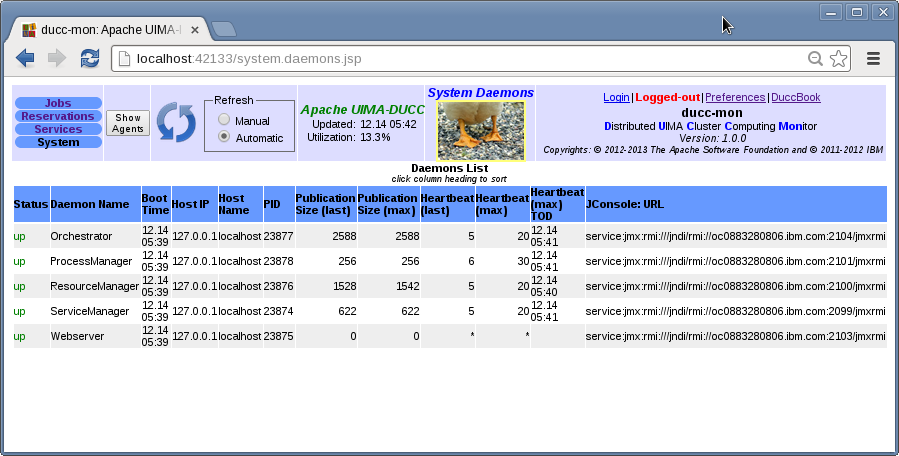
\includegraphics[width=90mm]{images/ducc-webserver/System-Daemons.png}
\caption{Sample Webserver Page}
\label{overflow}
\end{figure}

    Normally, the Web Server automatically fetches new data from DUCC and updates the display.
    This is controlled by setting one of the two refresh modes:
    \begin{itemize}
      \item Manual refresh.  In this mode, the browser windows are updated only by using the
        browser's refresh button, or the DUCC refresh button to the left in the header of
        each page.
      \item Automatic refresh. In this mode, the browser automatically fetches and displays
        new data.  The rate of refresh is currently fixed and cannot be configured.
    \end{itemize}
    
    There is a behavior difference between refresh and reload.
    \paragraph{Refresh}
    Refresh causes the current data on the page to be updated with the most
    current information in the Webserver's possession.  This is performed
    when the refresh button is clicked.
    \paragraph{Reload}
    Reload occurs when the enter key is pressed.  Reload causes not just the
    data to be updated but rather the entire page is replaced.
    
    Two different table styles are supported:
    \begin{itemize}
      \item Scroll, and
      \item Classic.
    \end{itemize}
    Table styles are switched using the {\em Preferences} link.

    \paragraph{Scroll Mode}  When {\em scroll table style} is the preference, a scroll bar is
    shown to the right, within the main window.  The scroll bar allows scrolling to be restricted to the data
    display, leaving column and DUCC headers in place.  In this mode any column may be sorted
    simply by clicking on it.
    
    With respect to sorting, any specified sort is remembered for refresh
    but forgotten for reload.  Sorting is permitted when either manual
    or automatic refresh mode is selected.
    
    The column sort order is maintained until the page is reloaded.

	Note that not all pages have a scroll version - some only have a classic version.
	
    \paragraph{Classic Mode}  When {\em classic table style} is the preference, the
    main data may extend below the bottom of the page and it will be necessary to use the browser's scroller on the right
    to access it.  The column headers and DUCC header scrolls off when doing this.  Columns
    may be sorted in this mode but it is necessary to first switch to ``Manual'' refresh mode to
    prevent browser refreshes during sorting and display of data. 
    
    With respect to sorting, any specified sort is forgotten for refresh
    and reload.  Sorting is only permitted when manual refresh mode is
    selected.
    
    The column sort order is maintained until the page is refreshed or reloaded.

\begin{figure}[ht!]
\centering
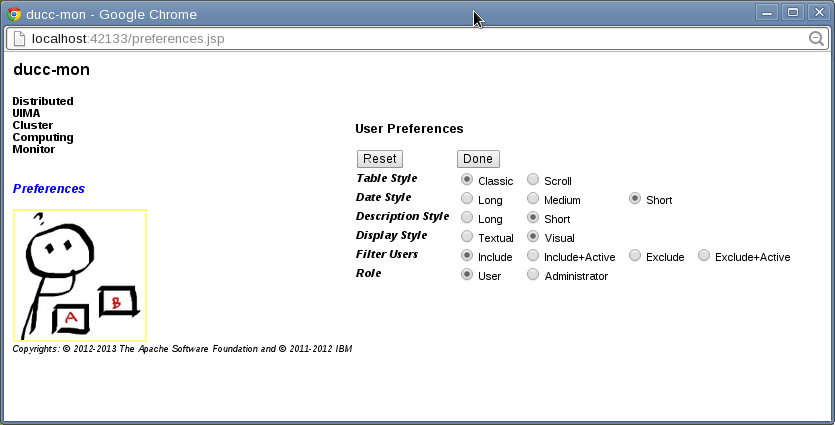
\includegraphics[width=90mm]{images/ducc-webserver/Preferences.png}
\caption{Preferences Page}
\label{overflow}
\end{figure}

% Create well-known link to this spot for HTML version
\ifpdf
\else
\HCode{<a name='DUCC_WS_COMMON'></a>}
\fi
    \section{Common Links}

        Every page contains a common header containing links and controls. The links permit navigation
        to other content at the site. The controls provide page-wise configuration of the content at
        that page.

        The following links are available on every page of the web server: 

        \begin{description}
          \item[Authentication] \hfill \\ 
            Authentication is needed in order to cancel jobs and reservations, to create a
            reservation, and to perform administration. It is not required to simply view the pages.

            \begin{itemize}
              \item Login - Authenticate and start a session with the Web Server.             
              \item Logout - Terminate the Web Server session 
            \end{itemize}

          \item[Preferences]
            The following preferences may be set:
            \begin{description}
              \item[Table Style] This selects ``scroll'' or ``classic'' display, as
                described above.
              \item[Date Style] This selects long, medium, or long formats for dates.
              \item[Description Style] This selects long or short formats for the various
                description fields.
              \item[Filter Users] This controls the ``filter'' box near the middle of
                the header on each page.  It allows various levels of inclusion and
                exclusion of active or completed work for the filtered users.
              \item[Role] This allows selection of ``User'' or ``Administrator'' roles.
                This protects registered DUCC administrators from accidentally affecting
                other people's work.
            \end{description}
            
          \item[DuccBook] \hfill \\
            This is a link to the HTML version of the document you are reading.

          \item[Jobs] \hfill \\
            This navigates to the Jobs page, showing all the jobs in the system.

          \item[Reservations] \hfill \\
            This navigates to the Reservations page, showing all the reservations
            in the system and provides a button that can be used to request new reservations. 

          \item[Services] \hfill \\
            This navigates to the Services page, showing all the services in the
            system.

          \item[System] \hfill \\
            This opens a sub-menu with system-related links:
            \begin{itemize}
              \item Administration - This opens a page with administrative functions. 
              \item Classes - This shows all the scheduling classes defined to the system. 
              \item Daemons - This shows the status of DUCC's management processes. 
              \item DuccBook - This manual. 
              \item Machines - This shows the status of all the ducc worker nodes. 
            \end{itemize}
      \end{description}              

      % Create well-known link to this spot for HTML version
      \ifpdf
      \else
      \HCode{<a name='DUCC_WS_JOBS'></a>}
      \fi
      % 
% Licensed to the Apache Software Foundation (ASF) under one
% or more contributor license agreements.  See the NOTICE file
% distributed with this work for additional information
% regarding copyright ownership.  The ASF licenses this file
% to you under the Apache License, Version 2.0 (the
% "License"); you may not use this file except in compliance
% with the License.  You may obtain a copy of the License at
% 
%   http://www.apache.org/licenses/LICENSE-2.0
% 
% Unless required by applicable law or agreed to in writing,
% software distributed under the License is distributed on an
% "AS IS" BASIS, WITHOUT WARRANTIES OR CONDITIONS OF ANY
% KIND, either express or implied.  See the License for the
% specific language governing permissions and limitations
% under the License.
% 

    \section{Jobs Page}
    \label{sec:ws.jobs-page}
        The Web Server's home page is also the Jobs page. This page has links to all the rest of the content 
        at the site and shows the status of all the jobs in the system. 
    
        The Jobs page contains the following columns: 

        \begin{description}

            \item[Id] \hfill \\
              This is the ID as assigned by DUCC. This field is hyperlinked to a
              \hyperref[sec:ws-job-details]{Job Details} page for that job that shows the breakdown of
              all the processes assigned to the job and their state.
              
            \item[Start] \hfill \\
              This is the time the Job is accepted into DUCC.
              
            \item[Duration] \hfill \\
              This shows two times.  In green the length of time the job has been running.  In black is
              the estimated time of completion, based on current resources and remaining work.  When
              the job completes, the time shown is the total elapsed time of the job.
                            
            \item[User] \hfill \\
              This is the userid of the job owner.
              
            \item[Class] \hfill \\
              This is the resource class the job is submitted to.
              
            \item[State] \hfill \\
              This shows the state of the job.  The normal job progression is shown below, with an
              explanation of what each state means.
              \begin{description}
                  \item[Received] - The job has been vetted, persisted, and assigned a unique ID. 
                  \item[WaitingForDriver] - The job is waiting for the Job Driver to initialize. 
                  \item[WaitingForServices] - The job is waiting for verification from the
                    Service Manager that required services are started and responding.  This may
                    cause DUCC to start services if necessary.  In that even this state will
                    persist until all pre-requisite services are ready.
                  \item[WaitingForResources] - The job is waiting to be scheduled. In busy
                    systems this may require preemption of existing work.  In that case this
                    state will persist until preemption is complete.
                  \item[Initializing] - The job initializing. Usually this
                    is the UIMA-AS initialization phase.  In the default configuration, only
                    two (2) processes are allocated by the Resource Manager.  No additional
                    resources are allocated until at least one of the new processes successfully
                    completes initialization.  Once initialization is complete the Resource Manager
                    will double the number of allocated processes until the user's fair share of
                    the resources is attained.
                  \item[Running] - At least one process is now initialized and running. 
                  \item[Completing] - The last work item has completed and DUCC is freeing resources.
                    If the job had many resources allocated at the time the job exited this state
                    will persist until all allocated resources are freed.
                  \item[Completed] - The job is complete. 
              \end{description}
                  
            \item[Reason or Extraordinary Status] \hfill \\

              % See this structure:
              % org.apache.uima.ducc.transport.event.common.IDuccCompletionType
              
              This field contains miscellaneous information pertaining to the job.  If the job exits
              the system for any reason, that reason is shown here.  If the job's pre-requisite
              services are unavailable (or ailing) that fact is displayed here.  If there is a
              job monitor running, that fact is shown here.  Most of the values for this field
              support ``hovers'' containing additional information about the reason.
         
              \begin{description}
                  \item[EndOfJob] - The job and completed ran with no errors. 
                  \item[Error] - All work items are processes but at least one had an error. 
                  \item[CanceledByDriver] - The Job Driver (JD) terminated the job. The reason for
                    termination is seen by hovering over the text with your mouse.
                  \item[CanceledBySystem] - The job was canceled because DUCC was shutdown. 
                  \item[CanceledBySser] - The job owner or DUCC administrator canceled the job. 
                  \item[Cancel Pending] - The job has been canceleled and is not yet fully evicted
                    from the system.
                  \item[DriverInitializationFailure] - The Job Deiver (JD) process is unable to initialize. Hover over 
                    the field with your mouse for details (if any are available), and check your JD log. 
                  \item[DriverProcessFailed] - The Job Driver (JD) process failed for some reason. Hover over the 
                    field with your mouse for details (if any), and check your JD log. 
                  \item[MonitorActive] The job has a console monitor active.  This is enabled with the
                    job's ``wait\_for\_completion'' parameter on job submission.
                  \item[ServicesUnavailable] - The job declared a dependency on one or more services, and the 
                    Service Manager (SM) cannot find or start the required service. 
                  \item[Premature] - The job was terminated for some unknown reason before all work items were 
                    processed. Check the JP logs for details. 
                  \item[ProcessInitializationFailure] - Too many processes failed during
                    initialization and the job was canceled by DUCC.  Check the JP logs for the
                    reason.
                  \item[ProcessFailure] - Too many processes failed while running and DUCC canceled
                    the job.  Check the JP logs for the reason.
                  \item[ResourcesUnavailable] - The Resource Manager (RM) is unable to allocate resources for 
                    the job. For non-preemptable jobs this could be because the limit on that type of allocation is 
                    reached, or all the nodes are already allocated and work cannot be preempted to make space for 
                    it. For all jobs, it could be because the job class is invalid. 
                    \item[{\em service\_name}] If there is a service name in this field it indicates the job is
                      dependent on the service but the service is not responding to the Ducc Service Monitor's
                      pinger.
              \end{description}

            \item[Services] \hfill \\
              This is the number of services the job has declared dependencies on.  There is a ``hover'' that
              shows the ids of the services, if any.

            \item[Processes] \hfill \\
              This is the number of processes currently assigned to the job.

            \item[Init Fails] \hfill \\
              This is the total number of initialization failures experienced by the job. This
              field is hyperlinked to pages with log excerpts highlighting the specific failures.
              
            \item[Run Fails] \hfill \\
              This is the total number of process failures experienced by the job. This field is
              hyperlinked to pages with log excerpts highlighting the specific failures.
              
            \item[Pgin] This is the number of page-in events, over all processes, on the machines
              running the job.

            \item[Swap] This is the total swap space, over all the processes, being used by the job.

            \item[Size] \hfill \\
              This is the declared memory size of the job
              
            \item[Total] \hfill \\
              This is the total number of work items declared by the job.
              
            \item[Done] \hfill \\
              This is the total number of work items successfully completed for the job.
              
            \item[Error] \hfill \\
              This is the total number of exceptions thrown or other errors experienced by work
              items. This field is hyperlinked to pages containing log excerpts highlighting
              the failures.
              
            \item[Dispatch] \hfill \\
              This is the total number CASs that are currently dispatched. 

              This usually represents the quantity derived from the following formula:
\begin{verbatim}              
     min( (initialized.processes * threads.per.process), (incomplete.work.items - errors) )
\end{verbatim}

              The actual number is a measured number, not a calculated number, and may differ
              slightly from the formula if the measurement is taken immediately after process
              start-up, or in the time between a work item completing and a new one being
              dispatched.
              
            \item[Retry] \hfill \\
              This is the number of CASs that were retried for any reason.  Reasons for retry
              include preemption for fair-share, work-item timeout, or error conditions.

              Note: If a work item in any process fails, the entire process is considered
              suspect, and all work-items in the process are terminated.  Work items in the
              process which did not have errors are re-dispatched (retried) to a different
              process.
              
            \item[Preempt] \hfill \\
              This is the total number of processes that have been preempted to make room for
              other work due to Fair Share.
              
            \item[Description] \hfill \\
              This is the description string from the $--$description string from submit.
            \end{description}

    \begin{figure}[ht!]
    \centering
    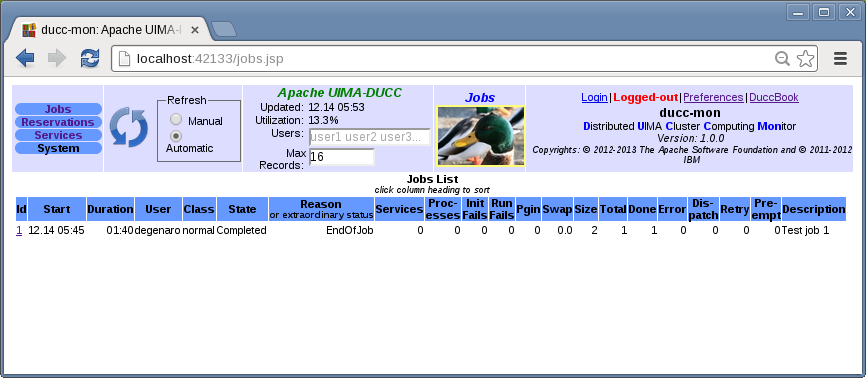
\includegraphics[width=90mm]{images/ducc-webserver/Jobs.png}
    \caption{Jobs Page}
    \end{figure}
            


      % Create well-known link to this spot for HTML version
      \ifpdf
      \else
      \HCode{<a name='DUCC_WS_JOB_DETAILS'></a>}
      \fi
      % 
% Licensed to the Apache Software Foundation (ASF) under one
% or more contributor license agreements.  See the NOTICE file
% distributed with this work for additional information
% regarding copyright ownership.  The ASF licenses this file
% to you under the Apache License, Version 2.0 (the
% "License"); you may not use this file except in compliance
% with the License.  You may obtain a copy of the License at
% 
%   http://www.apache.org/licenses/LICENSE-2.0
% 
% Unless required by applicable law or agreed to in writing,
% software distributed under the License is distributed on an
% "AS IS" BASIS, WITHOUT WARRANTIES OR CONDITIONS OF ANY
% KIND, either express or implied.  See the License for the
% specific language governing permissions and limitations
% under the License.
% 
  
    \section{Job Details Page}
    \label{sec:ws-job-details}

    This page shows details of all the processes that run in support of a job. 
    The information is divided among four tabs:
    \begin{description}
      \item[Processes] This tab contains details on all the processes for the job, both
        active, and defunct.
      \item[Work Items] This tab shows details for each individual work-item in the job.
      \item[Performance] This tab shows a performance break-down of all the UIMA analytics
        in the job.
      \item[Specification] This tab shows the job specification for the job.
      \end{description}
      
    \subsection{Processes}
    \label{subsec:ws-processes}
    The processes page contains the following columns:
    
    \begin{description}

        \item[Id] \hfill \\
          This is the DUCC-assigned numeric id of the process (not the Operating System's
          processid). Process 0 is always the Job Driver.          

        \item[Log] \hfill \\
          This is the log name for the process. It is hyperlinked to the log itself.

        \item[Size] \hfill \\
          This is the size of the log in MB. If you find you have trouble viewing the log
          from the Web Server it could be because it is too big to view in the server and needs to
          be read by some other means than the Web Server.  (It is not currently paged in by 
          the Web Server, it is read in full.)

        \item[Hostname] \hfill \\
          This is the name of the node where the process ran.

        \item[PID] \hfill \\
          This is the Unix process ID (PID) of the process.

        \item[State Scheduler] \hfill \\
          % The information comes from here:
          % State Scheduler: org.apache.uima.ducc.transport.event.common.IResourceState.ResourceState

          This shows the Resource Manager state of the job. It is one of:
          \begin{description}
              \item[Allocated] - The node is currently allocated for this job by the RM.
              \item[Deallocated] - The resource manager has deallocated the shares for the job on
                this node.
          \end{description}

        \item[Reason Scheduler or extraordinary status] \hfill \\
          \phantomsection\label{itm:job-details-sched}


          % The information comes from here:
          % Reason Scheduler: org.apache.uima.ducc.transport.event.common.IResourceState.ProcessDeallocationType
          This column provides a reason for the scheduler state, when the scheduler state is other than ``Allocated''. 
          These all have ``hovers'' that provide more information
          if it is available.

            \begin{description}          
                \item[AutonomousStop] - The process terminated unexpectedly of its own accord ("crashed", or
                  simply exited.) 

                \item[Exception] - The process is terminated by the JD exception handler. 

                \item[Failed] - The process is terminated by the Agent because the JP wrapper was able to detect and 
                  communicate a fatal condition (Exception) in the pipeline.. 
                  
                \item[FailedInitialization] - The process is terminated because the UIMA initialization step failed. 
                  
                \item[Forced] - The node is preempted by RM for other work because of fair share. 
                  
                \item[JobCanceled] - The job was canceled by the user or a system administrator. 
                  
                \item[JobCompleted] - The process is canceled because of DUCC restart. 
                  
                \item[JobFailure] - The job failure limit is exceeded, causing the job to be canceled by the JD.                    
                  
                \item[InitializationTimeout] - The UIMA initialization phase exceeded the configured timeout. 
                  
                \item[Killed] - The agent terminated the process for some reason. The ``Reason Agent'' field
                  should have more details in this case.
          
                \item[Stopped]	- The process was terminated by the Agent for some reason.  The hover should
                  contain more information.
                          
                \item[Voluntary] - The job is winding down, there's no more work for this node, so it stops. 
                  
                \item[Unknown] - None of the above. This is an exceptional condition, sometimes an
                  internal DUCC error. Check the JP and JD logs for possible causes..
            \end{description}

          \item[State Agent] \hfill \\
          \phantomsection\label{itm:job-details-state}

          % This state comes from here:
          % State Agent: org.apache.uima.ducc.transport.event.common.IProcessState.ProcessState
            This shows the DUCC Agent's view of the state of the process.
            \begin{description}
               \item[Starting] The DUCC process manager as issued a request to the assigned to
                 start the process.
               \item[Initializing] The process is initializing.  Usually this means the UIMA analytic
                 pipeline (Job Process) is executing it's initialization method.
              \item[Running] The Job Process has completed the initialization phase and is ready for, 
                or actively executing work.
              \item[Stopped] The DUCC Agent reports the process is stopped and (and has exited).
              \item[Failed] The DUCC Agent reports the process failed with errors.  This usually
                means that UIMA-AS has detected exceptions in the pipeline and reported them
                to the Job Driver for logging.
              \item[FailedInitialization] The process died during the UIMA initialization phase.
              \item[InitializationTimeout] The process exceeded the site's limit for time spent
                in UIMA initialization.
              \item[Killed] The DUCC Agent killed the process for some reason.  There are
                three rosins for this:
                \begin{enumerate}
                  \item The Job Processes failed to initialize,
                  \item The Job Process timed out during initialization,
                  \item The process Exocet's its allowed swap.
                \end{enumerate}
              \item[Abandoned] It is possible to cancel a specific process of a job.  Usually
                this is because it became ``stuck'' because of hardware failure.  It a process
                is killed in \hyperref[sec:cli.ducc-cancel]{this way}, the state is recoreded as {\em Abandonded}.
            \end{description}
            
          \item[Reason Agent] \hfill \\
          \phantomsection\label{itm:job-details-agent}

          This shows extended reason information if a process exited other than having run out
          of work to do.

            \begin{description}
              \item[AgentTimedOutWatingForORState] The DUCC Agent is expecting a state update
                from the DUCC Orchestrator.  Timer on this wait has expired.  This usually 
                indicates an infrastructure or communication problem.
              \item[Croaked] The process exited for no good or clear reason, it simply vanished.
              \item[Deallocated] WHAT IS THIS?
              \item[ExceededShareSize] The process exceeded it's declared memory size.
              \item[ExceededSwapThreshold] The process exceeded the configured swap threshold.
              \item[FailedInitialization] The process was terminated because the UIMA 
                initialization step failed.
              \item[InitializationTimeout] The process was terminated because the UIMA initialization
                step took too long.
              \item[JPHasNoActiveJob] This is set when an agent looses connectivity while its
                JPs are running. The job finishes (stopped or killed). The agent regains
                connectivity. The OR publish no longer includes the job but the agent still has
                processes running for that job. The agent kills ghost processes with the reason:
                JPHasNoActiveJob.
              \item[LowSwapSpace] The process was terminated because the system is about to run
                out of swap space.  This is a preemptive measure taken by DUCC to avoid exhaustion
                of swap, to effect orderly eviction of the job before the operating system starts
                its own reaping procedures.
              \item[AdministratorInitiated] The process was canceled by an administrator.
              \item[UserInitated] The process was canceled by the owning user.
            \end{description}
            
          \item[Time Init] \hfill \\
            This is the clock time this process spent in initialization.
            
          \item[Time Run] \hfill \\
            This is the clock time this process spent in executing, not including
            initialization.
            
          \item[Time GC] \hfill \\
            This is amount of time spent in Java Garbage Collection for the process.
            
          \item[Count GC] \hfill \\
            This is the number of garbage collections performed by the process.
            
          \item[Pgin] \hfill \\
            This is the number of page-in events on behalf of the process.

          \item[Swap] \hfill \\
            This is the amount of swap space on the machine being consumed by the process.

          \item[\%GC] \hfill \\
            Percentage of time spent in garbage collections by this process, relative to total of
            initialization + run times.
            
          \item[\%CPU] \hfill \\
            Currant CPU percent consumed by the process.  This will be $>$ 100\% on 
            multi-core systems if more than one core is being used.  Each core contributes
            up to 100\% CPU, so, for example, on a 16-core machine, this can be as high
            as 1600\%.
            
          \item[RSS] \hfill \\
            The amount of real memory being consumed by the process (Resident Storage Size)
            
          \item[Time Avg] \hfill \\
            This is the average time in seconds spent per work item in the process.
            
          \item[Time max] \hfill \\
            This is the minimum time in seconds spent per work item in the process.
            
          \item[Time min] \hfill \\
            This is the minimum time in seconds spent per work item in the process.
            
          \item[Done] \hfill \\
            This is the number of work items processed in this process.
            
          \item[Error] \hfill \\
            This is the number of exceptions processing work items in this process.
            
          \item[Retry] \hfill \\
            This is the number of work items that were retried in this process for any reason, excluding
            preemption.
            
          \item[Preempt] \hfill \\
            This is the number of work items that were preempted from this process, if
            fair-share caused preemption.
            
          \item[JConsole URL] \hfill \\
            This is a URL that can be used to connect via JMX to the processes, e.g. via
            jconsole.

      \end{description}
      
    \begin{figure}[ht!]
    \centering
    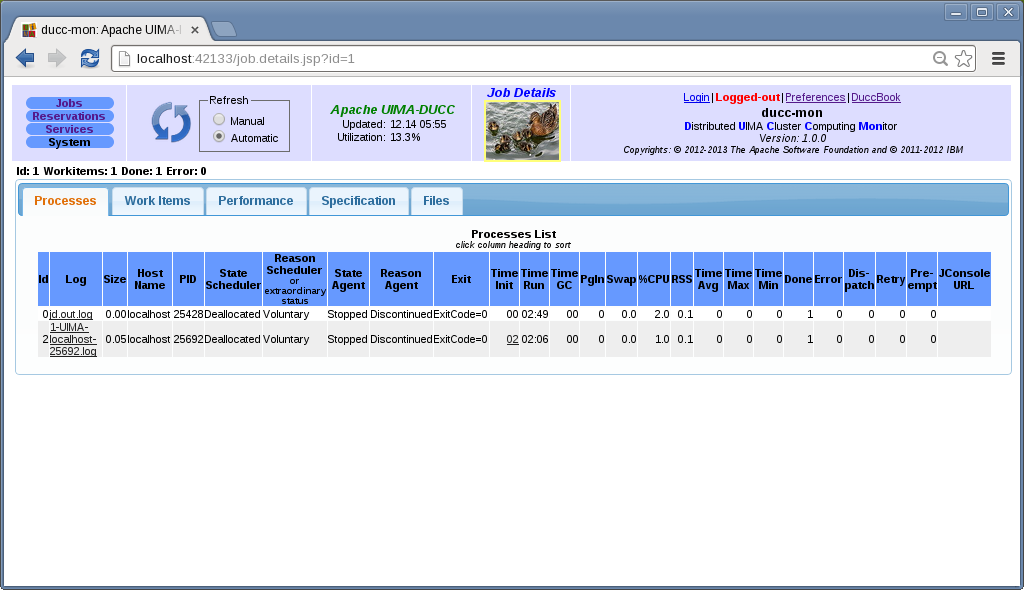
\includegraphics[width=90mm]{images/ducc-webserver/Job-Details-Processes.png}
    \caption{Processes Tab}
    \label{overflow}
    \end{figure}
    
   \subsection{Work Items}
   \label{subsec:ws-work-items}
   This tab provides details for each individual work item.  Columns include:

   % The data comes from here: org.apache.uima.ducc.common.jd.files.IWorkItemState.State    
   \begin{description}
     \item[SeqNo]  \hfill \\
       This is the sequence work items are fetched from the Collection Reader's
       getNext() method by the DUCC Job Driver.
     \item[Id]  \hfill \\
       This is the name of the work item.
     \item[Status]  \hfill \\
       The is the current state of the work item.  
       States include:
       \begin{description}
         \item[ended] The work item is complete.
         \item[error] The work item ended with errors.
         \item[lost] The work item was queued to ActiveMQ but never dequeued by
         any Job Process.
         \item[operating] The work item is current being executed.
         \item[retry] The work item is being retried.
         \item[start] The work item has been picked up for execution and DUCC is waiting
           for confirmation that it is running.
         \item[queued] The work item has been queued to ActiveMQ but not picked up by any
           Job Process yet.
       \end{description}
       If a work item has not yet been retrieved from the Collect Reader it does not show
       on this page.
     \item[Queuing Time (sec)]  \hfill \\
       The time spent in ActiveMQ after being queued, and before
       being picked up by a Job Process.
     \item[Processing Time (sec)]  \hfill \\
       The time spent processing the work item.
     \item[Node (IP)]  \hfill \\
       The node IP where the work item was processed.
     \item[Node (Name]  \hfill \\
       The node name where the work item was processed.
     \item[PID]  \hfill \\
       The Unix Process Id that the work item was processed in.
   \end{description}
    
    \begin{figure}[ht!]
    \centering
    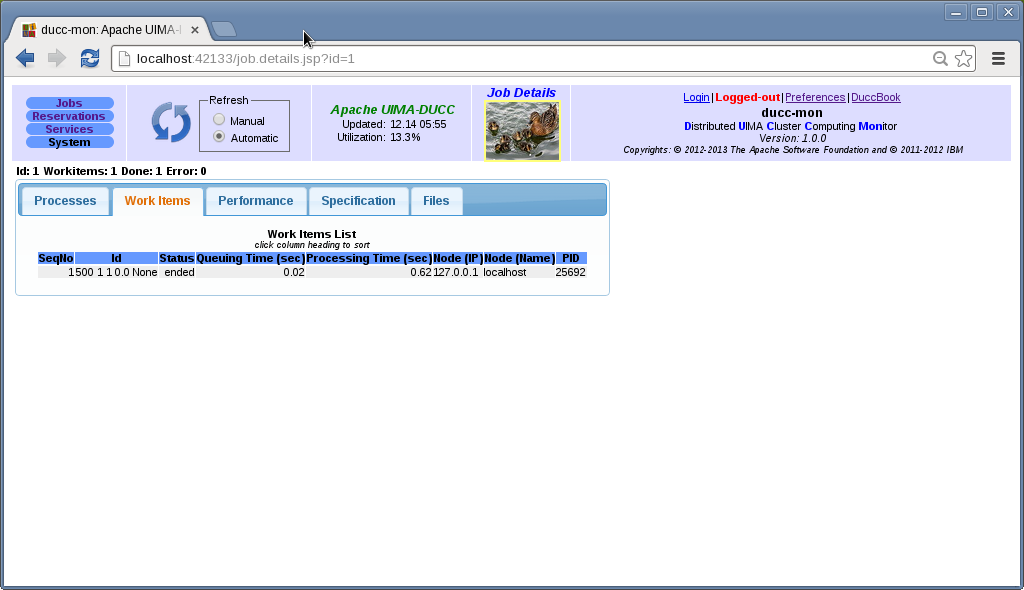
\includegraphics[width=90mm]{images/ducc-webserver/Job-Details-WorkItems.png}
    \caption{Work Items Tab}
    \label{overflow}
    \end{figure}  

   \subsection{Performance}
   \label{subsec:performance}
   This tab shows performance summaries of all the pipeline components.  The statistics
   are aggregated over all instances of each component in each process of the job.
   
   \begin{description}
     \item[Name]  \hfill \\
       The short name of the analytic.  The full name is shown in the command-line
       tool \hyperref[sec:cli.ducc-perf-stats]{ducc\_perf\_stats}
     \item[Total]  \hfill \\
       This is the total time in days, hours, minutes, and seconds taken by each
       component of the pipeline.
     \item[\% of Total]  \hfill \\
       This is the percent of the total usage consumed by this analytic.
     \item[Avg]  \hfill \\
       This is the average time spent by all the instances of the analytic.
     \item[Min]  \hfill \\
       This is the minimum time spent by any instance of the analytic.
     \item[Max]  \hfill \\
       This is the maximum time spent by any instance of the analytic.
   \end{description}
    
    \begin{figure}[ht!]
    \centering
    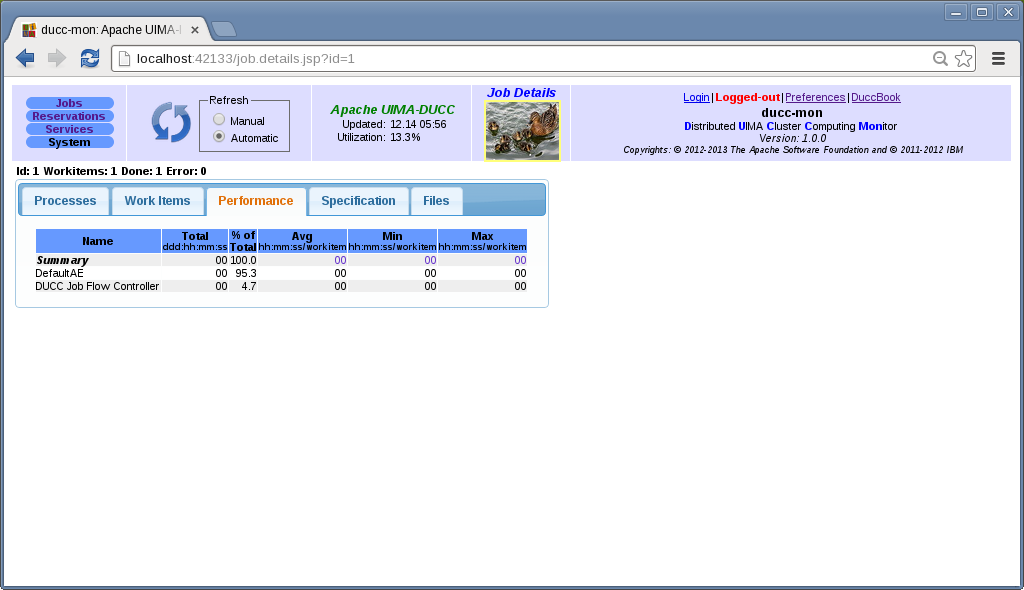
\includegraphics[width=90mm]{images/ducc-webserver/Job-Details-Performance.png}
    \caption{Performance Tab}
    \label{overflow}
    \end{figure}  
       
   \subsection{Specification}
   This tab shows the full job specification in the form of a Java Properties
   file.  This will include all the parameters specified by the user, plus those
   filled in by DUCC.
    
    \begin{figure}[ht!]
    \centering
    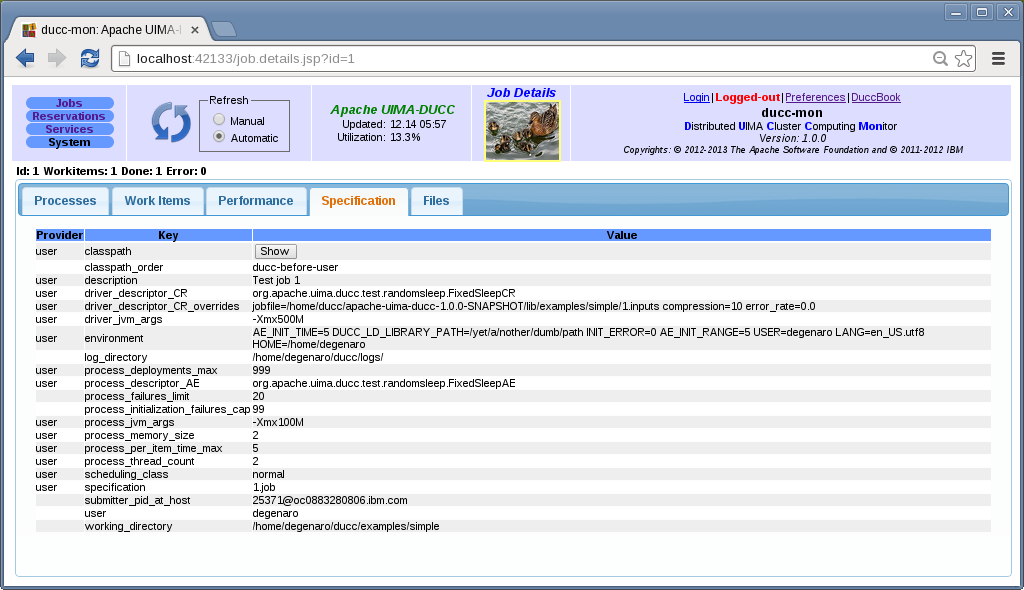
\includegraphics[width=90mm]{images/ducc-webserver/Job-Details-Specification.png}
    \caption{Specification Tab}
    \label{overflow}
    \end{figure}  

      % Create well-known link to this spot for HTML version
      \ifpdf
      \else
      \HCode{<a name='DUCC_WS_RESERVATIONS'></a>}
      \fi
      % 
% Licensed to the Apache Software Foundation (ASF) under one
% or more contributor license agreements.  See the NOTICE file
% distributed with this work for additional information
% regarding copyright ownership.  The ASF licenses this file
% to you under the Apache License, Version 2.0 (the
% "License"); you may not use this file except in compliance
% with the License.  You may obtain a copy of the License at
% 
%   http://www.apache.org/licenses/LICENSE-2.0
% 
% Unless required by applicable law or agreed to in writing,
% software distributed under the License is distributed on an
% "AS IS" BASIS, WITHOUT WARRANTIES OR CONDITIONS OF ANY
% KIND, either express or implied.  See the License for the
% specific language governing permissions and limitations
% under the License.
% 

\section{Reservation Page}
\label{sec:ws-reservations}

This page shows details of all reservations.  There are two types of reservations: {\em managed}
and {\em unmanaged.}.

A {\em managed reservation} is a reservation whose process is fully managed by DUCC.  This process
is any arbitrary process and is submitted with the
\hyperref[sec:cli.ducc-process-submit]{ducc\_process\_submit} CLI.  The lifetime of the reservation
starts at the time DUCC assigns a unique ID, and ends when the process terminates for any reason.

An {\em unmanaged reservation} is essentially a sandbox for the user.  DUCC starts no processes
in the reservation and manages none of the processes which run on that node.  The lifetime of the
reservation starts at the time DUCC assigns a unique ID, and ends when the submitter or system
administrator cancels it.  {\em Managed reservations} can potentially last an indefinite
period of time.

The Reservations page contains the following columns: 
\begin{description}

\item[Id] \hfill \\
  This is the unique DUCC numeric id of the reservation as assigned when the reservation is made.
  If this is a {\em managed} reservation, the ID is hyperlinked to a
  \hyperref[sec:ws-managed-reservation-details]{Managed Reservation Details} page with extended
  details on the process running in the reservation.

\item[Start] \hfill \\
  This is the time the reservation was mode.
  
\item[End] \hfill \\
  This is the time the reservation was canceled or otherwise ended.
  
\item[User] \hfill \\
  This is the userid if the person who made the reservation.
  
\item[Class] \hfill \\
  This is the scheduling class used to schedule the reservation.
  
\item[Type] \hfill \\
  This is the reservation type, {\em managed} or {\em unmanaged}, as described 
  \hyperref[sec:ws-reservations]{above}.

\item[State] \hfill \\
  % 1. org.apache.uima.ducc.transport.event.common.IDuccState
  This is the status of the reservation. Values include: Received - Reservation
  has been vetted, persisted, and assigned unique Id.
  \begin{description}
  \item[Assigned] - The reservation is active. 
  \item[Completed] - The reservation has been terminated.
  \item[Received] - The Reservation has been vetted, persisted, and assigned a unique ID.
  \item[WaitingForResources] - The reservation is waiting for the Resource Manager to find and 
    schedule resources. 
  \end{description}

\item[Reason] \hfill \\

  % 2. org.apache.uima.ducc.transport.event.common.IDuccCompletionType

  If a reservation is not active, this shows the reason.  Note that for
  {\em unmanaged reservations}, even if the user has processes running in the
  reservation, DUCC does NOT attempt to terminate those processes (hence, ``unmanaged''.)

  For {\em managed reservations}, DUCC does terminate the associated process.

  \begin{description}
  \item[CanceledBySystem] - In the case of the special JobDriver reservation, this is
    canceled by DUCC and reestablished on reboot; hence the state is a result of DUCC
    having been restarted.

    In all other cases, it is a result of DUCC being restarted {\em COLD}.  When
    DUCC is started {\em COLD}, all previous reservations are canceled.  (When DUCC
    is started {\em WARM}, the default, previous reservations are preserved.)
  \item[CanceledByAdmin] - The DUCC administrator released the reservation. 
  \item[CanceledByUser] - The reservation owner released the reservation. 
  \item[ResourcesUnavailable] - The Resource Manager was unable to find free or freeable resources 
    match the resource request. 
  \item[ProgramExit] - The reservation is a {\em managed} reservation and the associated
    process has exited.
  \end{description}

\item[Allocation] \hfill \\
  This is the number of resources (shares for FIXED policy reservations, processes for
  RESERVE policy reservations) that are allocated.

\item[UserProcesses] This is the number of processes owned by the user running in all
  shares of the reservation.  
  
  Note that even for {\em unmanaged} reservations, the DUCC agent tracks processes owned
  by the user and reports on them.  This allows better identification and management of
  abandoned reservations.

\item[Size] \hfill \\
  The memory size in GB of the each allocated unit.  This is the amount of memory that
  was {\em requested}.  In the case of RESERVE policy reservations, that actual memory
  of the reserved machine may be greater.
  
\item[Host Names] \hfill \\
  The node names of the machines where the resources are allocated.
  
\item[Description] \hfill \\
  This is the description string from the --description string from submit.
\end{description}

    \begin{figure}[ht!]
    \centering
    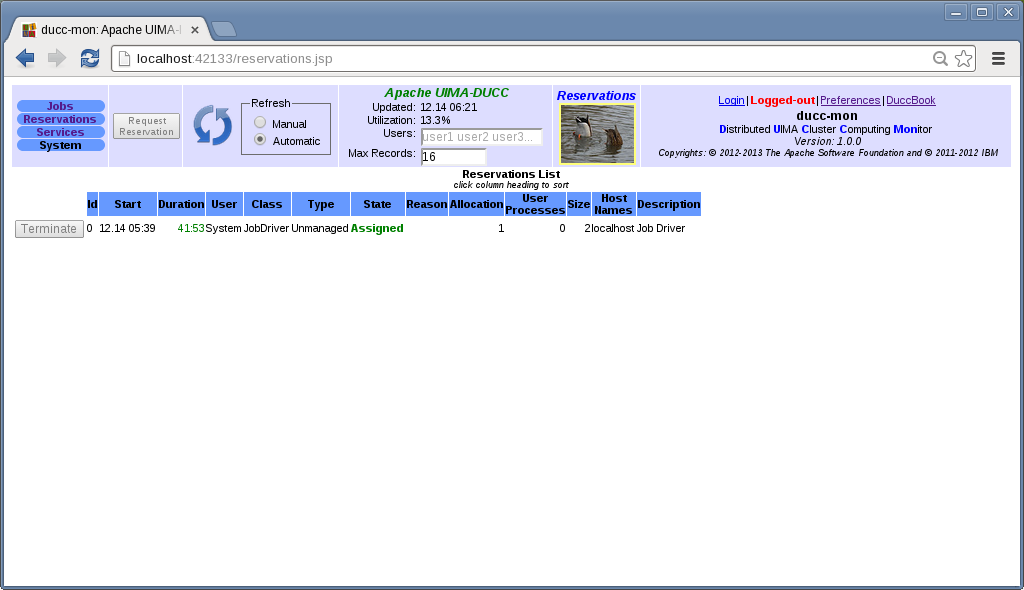
\includegraphics[width=90mm]{images/ducc-webserver/Reservations.png}
    \caption{Reservations Page}
    \label{overflow}
    \end{figure}

      % Create well-known link to this spot for HTML version
      \ifpdf
      \else
      \HCode{<a name='DUCC_WS_RESERVATIONS_DETAILS'></a>}
      \fi
      % 
% Licensed to the Apache Software Foundation (ASF) under one
% or more contributor license agreements.  See the NOTICE file
% distributed with this work for additional information
% regarding copyright ownership.  The ASF licenses this file
% to you under the Apache License, Version 2.0 (the
% "License"); you may not use this file except in compliance
% with the License.  You may obtain a copy of the License at
% 
%   http://www.apache.org/licenses/LICENSE-2.0
% 
% Unless required by applicable law or agreed to in writing,
% software distributed under the License is distributed on an
% "AS IS" BASIS, WITHOUT WARRANTIES OR CONDITIONS OF ANY
% KIND, either express or implied.  See the License for the
% specific language governing permissions and limitations
% under the License.
% 
\section{Managed Reservation Details Page}
\label{sec:ws-managed-reservation-details}

This page shows details of the processes which run in a managed reservation.  The
information is divided between two tabs:

   \begin{description}
       \item[Processes] This tab contains details on all the proceses contained in the
         reserved space.
       \item[Specification] This tab shows the specification for the process.
   \end{description}  

   \subsection{Processes}
   \label{sec:ws-manres-processes}

   The processes page contains the following columns:
   \begin{description}
      \item[ID] \hfill \\
        This is the DUCC-assigned numeric id of the process.  This format of this
        id is two numbers:
\begin{verbatim}
    RESID.SHAREID
\end{verbatim}
        Here, the {\em RESID} is the reservation ID.  The {\em SHAREID} is the 
        share ID assigned by the Resource Manager.  Together these form a unique
        ID for each process that runs in the reservation.
        
        Note: The current version of DUCC supports only one process per managed
        reservation.  Future versions are expected to support multiple processes
        within a single managed reservation.
        
      \item[Log] \hfill \\
        This is the log name for the process. It is hyperlinked to the log itself.
        
      \item[Size] \hfill \\
        This is the size of the log in MB. If you find you have trouble viewing the log
        from the web server it could be because it is too big to view in the browser.
        
      \item[Hostname] \hfill \\
        This is the name of the node where the process is running (or ran).
        
      \item[PID] \hfill \\
        This is the Unix process ID (PID) of the process.
        
      \item[State Scheduler] \hfill \\
        This shows the Resesource Manager state of the job. It is one of:
        
        \begin{description}
            \item[Allocated] - The node is still allocated for this job by the RM.
            \item[Deallocated] - The resource manager has deallocated the shares for the job on
              this node.
        \end{description}
        
      \item[Reason Scheduler or Extraordinary Status] \hfill \\
        These are the same as for the \hyperref[itm:job-details-sched]{job details.}

      \item[State Agent] \hfill \\
        These are the same as for the \hyperref[itm:job-details-state]{job details.}

      \item[Reason Agent] \hfill \\
        These are the same as for the \hyperref[itm:job-details-agent]{job details.}

      \item[Time Run] \hfill \\
        The current duration of the reservation, or total duration if it has 
        terminated.
        
      \item[RSS] \hfill \\
        The amount of real memory being consumed by the process (Resident Storage Size)

   \end{description}

   \subsection{Specification}
   \label{sec:ws-service-specification}
   This tab shows the full job specification in the form of a Java Properties
   file.  This will include all the parameters specified by the user, plus those
   filled in by DUCC.
        


      % Create well-known link to this spot for HTML version
      \ifpdf
      \else
      \HCode{<a name='DUCC_WS_SERVICES'></a>}
      \fi
      % 
% Licensed to the Apache Software Foundation (ASF) under one
% or more contributor license agreements.  See the NOTICE file
% distributed with this work for additional information
% regarding copyright ownership.  The ASF licenses this file
% to you under the Apache License, Version 2.0 (the
% "License"); you may not use this file except in compliance
% with the License.  You may obtain a copy of the License at
% 
%   http://www.apache.org/licenses/LICENSE-2.0
% 
% Unless required by applicable law or agreed to in writing,
% software distributed under the License is distributed on an
% "AS IS" BASIS, WITHOUT WARRANTIES OR CONDITIONS OF ANY
% KIND, either express or implied.  See the License for the
% specific language governing permissions and limitations
% under the License.
% 

    \section{Services Page}
    \label{ws:services-page}
        This page shows details of all services.           

        The Services page contains the following columns: 
        \begin{description}

            \item[Id] \hfill \\
              This is the unique numeric DUCC id of the service.  This ID is hyperlinked to a
              \hyperref[sec:ws-service-details]{Service Details} page with extended
              details on the service.  Note that for some types of services, DUCC may not
              know more about the service than is shown on the main page.

            \item[Name] \hfill \\
              This is the unique service endpoint of the service.  
              
            \item[Type] \hfill \\
              This is the service type, which is one of
              \begin{itemize}
                \item Registered
                \item Ping-Only
              \end{itemize}
              
            \item[State] \hfill \\
              This is the state of the service with respect to the service manager.  It is a
              consolidated state over all the service instances.  Valid states are
              \begin{description}
                \item[Available] At least one service instance is responding to the service
                  pinger, indicating it is functional.
                \item[Initializing] No service instances are available for use yet but at least one instance
                  is in its UIMA {\em initializing} phase.
                \item[Waiting] At least one service instance is in Running state, potentially available for use,
                  but no response has been received from the service pinger.  This usually occurs during the
                  start-up of a service.  If a service stops responding to its pinger after becoming
                  available, the state can regress to Waiting.
                \item[NotAvailable] No service instance is running or initializing. 
                \item[Stopping] The service has been stopped for some reason, but not all 
                  instances have terminated.  This is an intermediate state between Available and
                  NotAvailable to signify that the service is no longer available but not all its
                  resources have been returned yet.
              \end{description}

              DUCC will start dependent jobs ONLY if it's services are in state Available.  Otherwise
              DUCC attempts to start the service, and if successful, allows the job to start.  

              If a job is already running and a service becomes other than Available, the
              \hyperref[sec:ws.jobs-page]{jobs page} indicates the service is not available but the job is 
              allowed to continue.
              
            \item[Pinger] \hfill \\
              This indicates whether the Service Manager is running a pinger for the service.  This column
              does not imply the ping is successful; see the ``health'' column for ping status.
              
            \item[Health] \hfill \\
              {\em Health} is a status returned by each pinger and is the result of that pinger's
              evaluation of the state of the service.  It is shown as on of
              \begin{itemize}
                \item {\em Good}
                \item {\em Poor}
              \end{itemize}
              Both terms are highly subjective.  Pingers may return a summary of the underlying
              data used to label a service as good or bad.  That status is shown as a hover over
              this field.
              
            \item[Instances] \hfill \\
              This is the number of instances (processes) currently registered for the service.  

            \item[Deployments] \hfill \\
              This is the number of actual instances deployed for the service.  Note that this may
              be greater, or less, than the number of registered instances, if the service owner
              decides to temporarily start or stop additional instances.

            \item[User] \hfill \\
              This is the userid of the service owner.
              
            \item[Class] \hfill \\
              This is the scheduling class the service is running in. 
              
              If a service is registered as ``ping-only'', no resources are allocated for it.  This
              is shown as a class of {\tt ping-only}.
              
            \item[Size] \hfill \\
              This is the memory size, in GB, of each service instance

            \item[Jobs] \hfill \\
              This is the number of jobs currently using the service.  The IDs of the jobs are
              shown as hovers over this field.

            \item[Services] \hfill \\
              Services may themselves depend on other services.  This field shows the number of
              services dependent on this service.  The dependent service IDs are shown with a 
              hover over the field.

            \item[Reservations] \hfill \\
              This field shows the number of
              managed reservations dependent on this service. The IDs of the managed reservations
              are shown as a hover over the field.

              
            \item[Description] \hfill \\
              This is the description string from the --description string from submit.
        \end{description}


      % Create well-known link to this spot for HTML version
      \ifpdf
      \else
      \HCode{<a name='DUCC_WS_SERVICE_DETAILS'></a>}
      \fi
      % 
% Licensed to the Apache Software Foundation (ASF) under one
% or more contributor license agreements.  See the NOTICE file
% distributed with this work for additional information
% regarding copyright ownership.  The ASF licenses this file
% to you under the Apache License, Version 2.0 (the
% "License"); you may not use this file except in compliance
% with the License.  You may obtain a copy of the License at
% 
%   http://www.apache.org/licenses/LICENSE-2.0
% 
% Unless required by applicable law or agreed to in writing,
% software distributed under the License is distributed on an
% "AS IS" BASIS, WITHOUT WARRANTIES OR CONDITIONS OF ANY
% KIND, either express or implied.  See the License for the
% specific language governing permissions and limitations
% under the License.
% 
\section{Service Details Page}
\label{sec:ws-service-details}

This page shows details of the processes which implement. 

The information is divided between two tabs:

   \begin{description}
       \item[Processes] This tab contains details on all the proceses implementing
         the service, if any.
       \item[Specification] This tab shows the specification for the service.  
   \end{description}  

   \subsection{Processes}
   \label{sec:ws-services-processes}

   The processes page contains the following columns:
   \begin{description}
      \item[ID] \hfill \\
        This is the DUCC-assigned numeric id of the process.  This format of this
        id is two numbers:
\begin{verbatim}
    RESID.SHAREID
\end{verbatim}
        Here, the {\em RESID} is the reservation ID.  The {\em SHAREID} is the 
        share ID assigned by the Resource Manager.  Together these form a unique
        ID for each process that runs in the reservation.
                
      \item[Log] \hfill \\
        This is the log name for the process. It is hyperlinked to the log itself.
        
      \item[Size] \hfill \\
        This is the size of the log in MB. If you find you have trouble viewing the log
        from the web server it could be because it is too big to view in the browser.
        
      \item[Hostname] \hfill \\
        This is the name of the node where the process is running (or ran).
        
      \item[PID] \hfill \\
        This is the Unix process ID (PID) of the process.
        
      \item[State Scheduler] \hfill \\
        This shows the Resesource Manager state of the job. It is one of:
        
        \begin{description}
            \item[Allocated] - The node is still allocated for this job by the RM.
            \item[Deallocated] - The resource manager has deallocated the shares for the job on
              this node.
        \end{description}
        
      \item[Reason Scheduler or Extraordinary Status] \hfill \\
        These are the same as for the \hyperref[itm:job-details-sched]{job details.}

      \item[State Agent] \hfill \\
        These are the same as for the \hyperref[itm:job-details-state]{job details.}

      \item[Reason Agent] \hfill \\
        These are the same as for the \hyperref[itm:job-details-agent]{job details.}


      \item[Time Init] \hfill \\
        Most services are UIMA-AS services and therefore have an {\em initialization} phase
        to their lifetimes.  This field shows the time spent in that phase.

      \item[Time Run] \hfill \\
        The current duration of the reservation, or total duration if it has 
        terminated.
        
      \item[Time GC] \hfill \\
        This is amount of time spent in Java Garbage Collection for the process.

      \item[Pgin] \hfill \\
        This is the number of page-in events on behalf of the process.
        
      \item[Swap] \hfill \\
        This is the amount of swap space on the machine being consumed by the process.
        
      \item[\%CPU] \hfill \\
        Currnt CPU percent consumed by the process.  This will be $>$ 100\% on 
        multi-core systems if more than one core is being used.  Each core contributes
        up to 100\% CPU, so, for example, on a 16-core machine, this can be as high
        as 1600\%.

      \item[RSS] \hfill \\
        The amount of real memory being consumed by the process (Resident Storage Size)

      \item[JConsole URL] \hfill \\
        This is a URL that can be used to connect via JMX to the processes, e.g. via
        jconsole.

   \end{description}

   \subsection{Specification}
   \label{sec:ws-managed-reservation-specification}
   This tab shows the full job specification in the form of a Java Properties
   file.  This will include all the parameters specified by the user, plus those
   filled in by DUCC.
        
   The specification for a Service contains two types of entries:
   \begin{enumerate}
     \item Service specification properties, prefixed with ``svc''. These comprise
       the service specification that the Service Manager submits on behalf of
       a user in order to start registered services.
     \item Meta properties, prefixed with ``meta''.  This is the Service Manager's state
       record for the sesrvice as it is running.  In addition to state it contains
       properties required for service registration that are not used for
       service submission.
   \end{enumerate}
   


      % Create well-known link to this spot for HTML version
      \ifpdf
      \else
      \HCode{<a name='DUCC_WS_SYSTEM'></a>}
      \fi
      % 
% Licensed to the Apache Software Foundation (ASF) under one
% or more contributor license agreements.  See the NOTICE file
% distributed with this work for additional information
% regarding copyright ownership.  The ASF licenses this file
% to you under the Apache License, Version 2.0 (the
% "License"); you may not use this file except in compliance
% with the License.  You may obtain a copy of the License at
% 
%   http://www.apache.org/licenses/LICENSE-2.0
% 
% Unless required by applicable law or agreed to in writing,
% software distributed under the License is distributed on an
% "AS IS" BASIS, WITHOUT WARRANTIES OR CONDITIONS OF ANY
% KIND, either express or implied.  See the License for the
% specific language governing permissions and limitations
% under the License.
% 

\section{System  Details Page}
\label{sec:system-details}

This page shows information relating to the DUCC System itself:
\begin{description}
  \item[Administration]This displays system administrators and implements
    the interface to various administrative controls.
  \item[Classes] This shows the current system's scheduling class definitions.
  \item[Daemons] This shows the status of all DUCC processes.
  \item[DuccBook] This is a link to the book you are reading.
  \item[Machines] This shows details of all the machines in the DUCC cluster.
\end{description}

\subsection{Administration}

   This page has two tabs:
   \begin{description}   
     \item[Administrators] This shows the user-ids that are authorized to administer
       DUCC.  In addition to executing the ``Control'' functions described below,
       administrators may cancel any job, reservation, or service, and may modify
       services they do not own.  

       In order to perform administrative functions, the following must be satisfied:
       \begin{enumerate}
         \item The user is logged-in to the web server.
         \item The user is a registered administrator.
         \item The user has set the role as ``administrator'' in the DUCC Preferences
           page.  This is a safeguard so that administrators who are also users
           are less likely to inadvertently affect other people's jobs.
       \end{enumerate}
     \item[Control] Currently DUCC supports a single administrative control function
       via the web server: Stop new job submissions and re-enable them.  If submissions
       are blocked, all existing work runs normally, but no new work is accepted.
     \end{description}


\subsection{Classes}
This page shows the definitions of the DUCC scheduling classes.  The scheduling classes are
discussed in more detail in the \hyperref[sec:rm.job-classes]{Resource Manager} section.

\subsection{Daemons}
\label{sec:system-details.daemons}

This page shows the current state of all DUCC processes.  By default, only the administrative
processes, Orchestrator, ProcessManager, ResourceManager, ServiceManager, and Webserver are
shown.  A button in the upper left of the page titled ``Show Agents'' enables display of
the status of all the DUCC agents as well. (Agents are suppressed by default because the
page is expensive to render for large systems.)

The columns shown on this page include

   \begin{description}
      \item[Status] \hfill \\
        This indicates whether the daemon is running and broadcasting state {\em up},
        or not {\em down}.  
        
        All DUCC daemons broadcast a heartbeat containing process state.  If the Status
        is {\em down}, either the daemon is not functioning, or something is preventing
        state from reaching the web server via DUCC's ActiveMQ instance.

      \item[Daemon Name] \hfill \\
        This is the name of the process.

      \item[Boot Time] \hfill \\ 
        This shows the date and time of the latest boot of the specific process.
          
      \item[Host IP] \hfill \\ 
        This is the IP address of the processor where the process is running.

      \item[Host Name] \hfill \\ 
        This shows the hostname of the processor where the process is running.

      \item[PID] \hfill \\ 
        This is the Unix processid of the DUCC process.


      \item[Publication Size (last)] \hfill \\ 
        This shows the size of the most recent state publication of the process, in bytes.

      \item[Publication Size (max)] \hfill \\ 
        This shows the size of the largest state publication of the process, in bytes.

      \item[Heartbeat (last)] \hfill \\ 
        This shows the number of seconds since the last state publication for the process. 
         Large numbers here indicate potential cluster or DUCC problems.

      \item[Heartbeat (max)] \hfill \\ 
        This shows the longest delay since a state publication for the process was received
        at the web server.  Large numbers here indicate potential cluster or DUCC problems.

      \item[Heartbeat (max) TOD] \hfill \\ 
        This shows the time the longest delay of a state publication occurred.

      \item[JConsole URL] \hfill \\ 
        This is the jconsole URL for the process.

   \end{description}
      
\subsection{Machines}

This page shows the states of all the machines in the DUCC cluster.

The columns shown on this page include

   \begin{description}
      \item[Status] \hfill \\
        This shows the current state of a machine.  Values include:
        \begin{description}
          \item[defined] The node is in the DUCC
            \hyperref[sec:admin-ducc.nodes]{nodes file}, but no DUCC process has been
            started there, or else there is a communication problem and
            the state messages are not being delivered.
            \item[up] The node has a DUCC Agent process running on it and the
              web server is receiving regular heartbeat packets from it.
            \item[down] The node had a healthy DUCC Agent on it at some point
              in the past (since the last DUCC boot), but the web server has stopped
              receiving heartbeats from it. 

              The agent may have been manually shut down, may have crashed, or there
              may be a communication problem.

              Additionally, very heavy loads from jobs running the the node can cause
              the DUCC Agents heartbeats to be delayed.
        \end{description}


      \item[IP] \hfill \\
        This is the IP address of the node.

      \item[Name] \hfill \\
        This is the hostname of the node.

      \item[Reserve(GB) size] \hfill \\
        This is the largest reservation that can be made on this node.

        This is usually somewhat less than the physical memory size because it is 
        rounded down to the nearest \hyperref[chap:rm]{share quantum}.  The purpose of this
        column is to assist users in requesting the right size for full machine 
        reservations.

      \item[Memory(GB) total] \hfill \\
        This is the amount of memory, in GB, as reported by each machine.
        
        Usually the amount will be slightly less than the installed memory.  This is because
        a small bit of memory is usually reserved by the hardware for its own purposes.  For 
        example, a machine with 48GB of installed memory may report only 47GB available.

      \item[Swap(GB) in use] \hfill \\
        This is the total size in-use swap data.  DUCC shows any value greater than 0 in
        red as swapping can very significantly slow applications.  However, swap use does
        not always mean there is a performance problem.  This is flagged by DUCC simply
        as an alert of a potential problem

      \item[Alien PIDs] \hfill \\
        This shows the number of processes not owned by DUCC, the operating system, or
        jobs scheduled on each node.  The Unix Process IDS of these processes is displayed
        in a hover.

        DUCC preconfigures many of the standard operating 
        \hyperref[itm:props-rogue.process]{system process} and 
        \hyperref[itm:props-rogue.user]{userids}.  This list may be updated by each
        installation.

        A common cause of alien PIDs is errant process run in unmanaged reservations.  A
        user may reserve a machine for use as a sandbox.  If the reservation is released
        without properly terminating all the processes, they may linger.  When ducc 
        schedules the node for other purposes, significant performance penalties may be
        paid due to competition between the legitimately scheduled work and the leftover
        ``alien'' processes.  The purpose of this column is to bring attention to this situation.

      \item[Shares (total)] \hfill \\
        This shows the total number of scheduling share supported on this node.

      \item[Shares(in use)] \hfill \\
        This shows the total number of scheduling share in use on the node.

      \item[Heartbeat(last)] \hfill \\
        This shows the number of seconds since the last agent heartbeat from this machine.

      \end{description}
      





\part{Programming Model And Applications}
% 
% Licensed to the Apache Software Foundation (ASF) under one
% or more contributor license agreements.  See the NOTICE file
% distributed with this work for additional information
% regarding copyright ownership.  The ASF licenses this file
% to you under the Apache License, Version 2.0 (the
% "License"); you may not use this file except in compliance
% with the License.  You may obtain a copy of the License at
% 
%   http://www.apache.org/licenses/LICENSE-2.0
% 
% Unless required by applicable law or agreed to in writing,
% software distributed under the License is distributed on an
% "AS IS" BASIS, WITHOUT WARRANTIES OR CONDITIONS OF ANY
% KIND, either express or implied.  See the License for the
% specific language governing permissions and limitations
% under the License.
% 
\chapter{Building and Testing Jobs}

\section{Overview}

A DUCC job consists of two process types, a Job Driver process and one or more
Job Processes. These processes are connected together via UIMA-AS.
The Job Driver process wraps the job's Collection Reader (CR). The CR
function is to define the collection of Work Items to be processed.
The Collection Reader returns a small CAS for each Work Item containing a
reference to the Work Item data
The Job Driver uses the UIMA-AS client API to send Work Item CASes 
to the job's input queue. Job Processes containing the analytic pipeline are deployed
as UIMA-AS services and comsume CASes from the job input queue.

A basic job's analytic pipeline consists of an Aggregate Analysis Engine comprised by
the user specified CAS Multiplier (CM), Analysis Engine (AE) and CAS
Consumer (CC) components, along with a built-in DUCC Flow Controller.
The Work Item CAS is typically sent only to the CM and returned by
the Job Process when all child CASes produced by the CM have completed
processing; optionally the CR can configure Work Item CAS flow to go to the CC 
or to the AE \& CC to complete all processing for that Work Item.

	\begin{description}
	    \item[Note:] Although the Job Driver will receive back the Work Item CAS, 
	    there is no provision for any user code to receive the CAS. Therefore a
		Job Process typically adds no results to a Work Item CAS.
	\end{description}

   \subsection{Basic Job Process Threading Model}
   In addition to the pipeline definition of explicitly named CM, AE and CC components, the job
   specification also includes the number of pipeline threads to run in each
   Job Process (using the job specification parameter: process\_thread\_count).
   Each pipeline thread receives Work Items independently.

   DUCC creates an aggreate descriptor for the pipeline, and then creates a
   Deployment Descriptor for the Job Process which specifying the number
   of synchronous pipelines.
   
   \subsection{Alternate Pipeline Threading Model}
   Alternately a Job Process can be fully specified by a user submitted UIMA-AS
   Deployment Descriptor. Thus any UIMA-AS service deployment can be used as a
   Job Process. Here the parameter process\_thread\_count just defines
   how many Work Items CASes will be sent to each Job Process concurrently.
   
	\begin{description}
	    \item[Note:] In general a UIMA-AS service may be configured to
	    return child CASes; although child CASes returned from a Job Process will be
	    ignored by the Job Driver, there may be significant overhead in wasted
	    serialization and I/O.
	\end{description}

   \subsection{Overriding UIMA Configuration Parameters}
   UIMA configuration parameters in the CR, CM, AE or CC components can be overriden using
   job specification parameters: driver\_descriptor\_CR\_overrides, process\_descriptor\_CM\_overrides,
   process\_descriptor\_AE\_overrides and process\_descriptor\_CC\_overrides, respectively.

   Another approach is to use the {\em External Configuration Parameter Overrides} mechanism
   in core UIMA. External overrides is the only approach available for jobs submitted with
   a Deployment Descriptor.


\section{Collection Segmentation and Artifact Extraction}

UIMA is built around artifact processing. A classic UIMA pipeline starts with
a Collection Reader (CR) that defines collection seqmentation, extracts the artifacts
to be analyzed and puts them into the CASes to be delivered to subsequent analytic components. 
A CR designed for a specific data collection is highly reusable
for many different analytic scenarios.

A single CR supplying artifacts to a large number of analysis pipelines 
would be a bottleneck. Not only would artifact data need to be transported twice across
the compute cluster, but analysis results would be uselessly returned to the Job Driver.
To solve both of these problems, in a DUCC job the CR only sends a reference
to the artifacts in the Work Item CAS, and artifact data is read directly by the analysis pipeline.

In DUCC collection processing the role of collection segmentation is
implemented by the CR run in the Job Driver, while
artifact extraction and CAS initialization are implemented in the Cas Multiplier
(CM) run in the Job Process. The combination of a CR and associated CM 
should be highly reusable. 

\begin{description}
    \item[Note:] In many cases it is useful to reference multiple artifacts in a
      Work Item CAS. Both DUCC sample applications described below exhibit this design.
\end{description}

\section{CAS Consumer Changes for DUCC}

CAS Consumers in a UIMA pipeline may require changes for scale out into DUCC
jobs, to avoid scale out bottlenecks, to preserve collection level
processing, or to flush results at end-of-work-item processing.
   
	\begin{description}
	    \item[Federated ouput:] Scaled out DUCC jobs distribute artifact processing
	    to multiple pipeline instances. All instances of a CAS Consumer should have
	    independent access to the output target (filesystem, service, database, etc.).
	    \item[Singleton processing:] Collection level processing
	    requiring that all results go to a singleton process would usually be done as a 
            follow-on job, allowing
	    incremental progress; Job Process errors due to data-dependent analysis bugs
	    can often be fixed without invalidating completed Work Items, 
            enabling a restarted job to utilize the progress made by
	    previous job runs.
	    \item[Flushing cached data:] In some scenarios each Work Item delivered to a
	    pipeline can be considered an independent collection. If a CAS Consumer
	    caches data which needs to be flushed after processing the
	    last artifact for a Work Item, the Work Item CAS can be routed to the CAS Consumer after
	    the last artifact CAS is processed and used to trigger cache flushing.
	\end{description}


\section{Job Development for an Existing Pipeline Design}

Assuming that an existing job input-output design (CR, CM, CC) is to be reused, job
development is focussed on the Analysis Engine (AE) to be plugged in. Before deploying a new
AE in a multithreaded Job Process it is best to run it single threaded
(process\_thread\_count=1) to separate basic logic errors from threading
problems.

To debug a Job Process with eclipse, first create a debug configuration for a
"remote java application", specifying "Connection Type = Socket Listen" on some
free port P. Start the debug configuration and confirm it is listening on the specified port.
Then add to the job specification
process\_debug=port, where port is the value P used in the running debug configuration.

When the process\_debug parameter is specified, DUCC will only run a single Job Process
that will connect back to the eclipse debug configuration.


\section{Job Development for a New Pipeline Design}

A DUCC job is a UIMA application comprised of user code broken into a Collection
Reader running in the Job Driver and an Agreggate Analysis Engine (analysis pipeline) running in one 
or more Job Processes. Each Job Process may run multiple instances of the pipeline, each in a different
thread. The major components of the basic Job Process application are as follows:

\begin{itemize}
  \item User Collection reader - segments the input collection in to Work Items
  \item User CAS Multiplier - inputs a Work Item and segments it into artifacts (CASes)
  \item User Analysis Engine - processes the CASes
  \item User CAS Consumer - outputs results for each Work Item
  \item DUCC built-in Flow Controller - routes Work Item CASes to the CM and optionally to the CC or AE \& CC.
\end{itemize}

It is good if the CR+CM+CC combination can be reused for a broad range of AE.

\subsection{Collection Reader (CR) Characteristics}
A DUCC Job CR sends Work Item CASes to the Job Processes. These CASes contain references to the data
to be read by the Job Processes. Typically the CR Type System will be very small; in the DUCC sample
applications the CR Type System only contains the Workitem Feature Structure described below.

\begin{description}
    \item[Note:] It is important not to include the analytic Type System in the CR. These Type Systems 
can be quite large and will significantly increase the size of each Work Item CAS. 
The Job Driver process maintains a CAS pool which must be as large
as the total number of processing threads active in a job. 
\end{description}

\subsection{DUCC built-in Flow Controller}
\begin{sloppypar}
This flow controller provides separate flows for Work Item CASes and for CASes produced by the CM and/or AE.
Its behavior is controlled by the existence of a CM component, and then further specified by the
org.apache.uima.ducc.Workitem feature structure in the Work Item CAS.
\end{sloppypar}

When no CM is defined the Work Item CAS is simply delivered to the AE, and then to the CC if defined. 
Any CASes created by the AE will be routed to the CC.

With a defined CM, the Work Item CAS is delivered only to the CM, and then returned from the JP when processing
of all child CASes created by the CM and AE has completed. Work Item CAS flow can be further refined by the CR by
creating a org.apache.uima.ducc.Workitem feature structure and setting the setSendToLast feature to true,
or by setting the setSendToAll feature to true.

\subsection{Workitem Feature Structure}
In addition to Work Item CAS flow control features, the WorkItem feature structure includes other features that are useful
for a DUCC job application. Here is the complete list of features:

\begin{description}[labelindent=0.5in,leftmargin=0.5in]
  \item[sendToLast] (Boolean) - indicates the Work Item CAS be sent to the CC
  \item[sendToAll] (Boolean) - indicates Work Item CAS be sent to the AE and CC
  \item[inputspec] (String) - reference to Work Item input data
  \item[outputspec] (String) - reference to Work Item output data
  \item[encoding] (String) - useful for reading Work Item input data
  \item[language] (String) - used by the CM for setting document text language
  \item[bytelength] (Integer) - size of Work Item
  \item[blockindex] (Integer) - used if a Work Item is one of multiple pieces of an input resource
  \item[blocksize] (Integer) - used to indicate block size for splitting an input resource
  \item[lastBlock] (Boolean) - indicates this is the last block of an input resource
\end{description}

\subsection{Deployment Descriptor (DD) Jobs}
Job Processes with arbitrary aggregate hierarchy, flow control and threading can be fully specified
via a UIMA AS Deployment Descriptor. DUCC will modify the input queue to use DUCC's private
broker and change the queue name to correspond to the DUCC job ID.

\subsection{Debugging}
It is best to develop and debug the interactions between job application components as one, 
single-threaded UIMA aggregate. DUCC provides an easy way to accomplish this, for both basic
and DD job models, using the all\_in\_one specification parameter.

\begin{description}
    \item[all\_in\_one=local] When set to local, all Job components are run in the same
      single-threaded process, on the same machine as eclipse.
    \item[all\_in\_one=remote] With remote, the single-threaded process is run on a DUCC
      worker machine as a DUCC Managed Reservation. 
\end{description}

To debug an all\_in\_one job with eclipse, first create a debug configuration for a
"remote java application", specifying "Connection Type = Socket Listen" on some
free port P. Start the debug configuration and confirm it is listening on the specified port.
Then, before submitting the all\_in\_one job, add the argument process\_debug=port, 
where port is the value P used in the running debug configuration.


\chapter{Sample Application: Raw Text Processing}

\section{Application Function and Design}
This application expects as input a directory containing one or more flat text files, 
uses paragraph boundaries to segment the text into separate artifacts, 
processes each artifact with the OpenNlpTextAnalyzer, and writes
the results as compressed UIMA CASes packaged in zip files. Paragraph boundaries are defined as
two or more consecutive newline characters.

By default each input file is a Work Item. In order to facilitate processing scale out, 
an optional blocksize parameter can be specified that will be used to break larger 
files into multiple Work Items. Paragraphs that cross block boundaries are processed
in the block where they started. An error is thrown if a paragraph crosses two block
boundaries.

An output zip file is created for each Work Item. The CAS compression format is selectable as
either ZIP compressed XmiCas or UIMA compressed binary form 6 format. When compressed binary
is used, each zip file also contains the full UIMA Type System in ZIP compressed text.
CASes in UIMA compressed binary form 6 format have the same flexibility as an XmiCas in that
they can be deserialized into a CAS with a different, but compatible Type System.

By default any previously completed output files found in the output directory are preserved.
While Work Item processing is in progress the associated output files have "\_temp" appended to their
filenames, and any such incomplete output files are always ignored for subsequent jobs.

\section{Configuration Parameters}
The Collection Reader for this job is the DuccJobTextCR. It has the following configuration
parameters:

\begin{description}[labelindent=0.5in,leftmargin=0.5in]
    \item[InputDirectory] path to directory containing input files.
    \item[OutputDirectory] path to directory for output files.
    \item[IgnorePreviousOutput] (optional) boolean to ignore (overwrite) existing output files.
    \item[Encoding] (optional) character encoding of the input files.
    \item[Language] (optional) language of the input documents, i.e. cas.setDocumentLanguage(language).
    \item[BlockSize] (optional) integer value used to break larger input files into multiple Work Items.
    \item[SendToLast] (optional) boolean to route WorkItem CAS to last pipeline component. Is set to true for this application.
    \item[SendToAll] (optional) boolean to route WorkItem CAS to all pipeline components. Not used in this application.
\end{description}

The CAS Consumer is the DuccCasCC and has the following configuration parameters:

\begin{description}[labelindent=0.5in,leftmargin=0.5in]
  \item[XmiCompressionLevel] (optional) compression value if using ZIP compression. Default is 7, range is 0-9.
  \item[UseBinaryCompression] (optional) boolean to select UIMA binary CAS compression.
\end{description}

\section{Set up a working directory}
For this and the following sample program, create a working directory in a writable filesystem.

Copy to this directory the example job specification files:
\begin{verbatim}
   cp $DUCC_HOME/examples/sampleapps/descriptors/*.job .
\end{verbatim}

Copy a UIMA logger configuration file that suppresses tons of output from OpenNLP:
\begin{verbatim}
   cp $DUCC_HOME/examples/sampleapps/descriptors/ConsoleLogger.properties .
\end{verbatim}

Copy the executable code and resources for the DUCC sample application components:
\begin{verbatim}
   mkdir lib
   cp $DUCC_HOME/lib/uima-ducc/examples/uima-ducc-examples*.jar lib
\end{verbatim}

For reference the source code for DUCC sample applications is in \ducchome/examples/src,
with descriptors in \ducchome/examples/sampleapps/descriptors.

\section{Download and Install OpenNLP}
Download the OpenNLP source distribution from http://opennlp.apache.org and follow the directions in the
{\em UIMA Integration} section of the included documentation to build the UIMA pear file.
Then {\em install} the UIMA pear file in the working directory 
with the {\em runPearInstaller} script and
test it with the UIMA Cas Visual Debugger application.

A small modification of the installed OpenNLP descriptor file
is necessary for DUCC to run the component multithreaded. 
Edit {\em opennlp.uima.OpenNlpTextAnalyzer/desc/OpenNlpTextAnalyzer.xml}
and change the setting for {\em multipleDeploymentAllowed} from false to true.

\section{Get some Input Text}
Choose one or more flat text files in UTF8 format that only use newline characters,
{\em not CR-LF sequences}.
The text should be big enough to see the impact of DUCC job scale out.
We used test data from gutenberg.org at
\begin{verbatim}
   http://www.gutenberg.org/ebooks/search/?sort_order=downloads
\end{verbatim}
downloading 'Plain Text UTF-8' versions of {\em Moby Dick}, {\em War and Peace} and {\em The Complete Works of William Shakespeare} 
as flat text files in
a subdirectory `Books', and removing all 'CR' characters (0xD) as well as extraneous text.

\section{Run the Job}
The job specification, DuccRawTextSpec.job, uses placeholders to reference the working directory
and various operational components located there. As run below the placeholders are resolved
from environmental variables.

The job is submitted from the command line with the following:
\begin{verbatim}
   MyAppDir=$PWD \
   MyInputDir=$PWD/Books \
   MyOutputDir=$PWD/Books.processed \
   $DUCC_HOME/bin/ducc_submit -f DuccRawTextSpec.job
\end{verbatim}

The total size of the three txt files is 9.4Mbytes and with a blocksize of 100000 there are 100 Work Items. Each Job Process is 
configured to run 8 parallel OpenNLP pipelines. To examine the performance of processing with just a single Job Process, 
the job can be submitted as:

\begin{verbatim}
   MyAppDir=$PWD \
   MyInputDir=$PWD/Books \
   MyOutputDir=$PWD/Books.processed \
   $DUCC_HOME/bin/ducc_submit -f DuccRawTextSpec.job \
   --process_deployments_max 1
\end{verbatim}

\section{Job Output}
There will be an output zipfile for every Work Item, with zipfiles containing a compressed CAS for each document (paragraph) 
found in a Work Item. If UseBinaryCompression=true each zipfile will also contain the TypeSystem for the CASes. 
This is needed when deserializing these CASes into a different TypeSystem.

DuccTextCM finds 19245 paragraphs in the three txt files. If the output CASes are stored as 19245 uncompressed XMI files, the total size is 911MB. Using the default ZIP compressed XMI format and packed into 100 Work Item zip files, the total size is 165MB, a 5.5x compression. Using UIMA binary compressed format further reduces total size to 62MB.

This output data will be used as input data for the following CAS input processing sample application.

\section{Job Performance Details}
DUCC captures a number of process performance metrics.
\hyperref[fig:OpenNLP-Process-Measurements]{Figure ~\ref{fig:OpenNLP-Process-Measurements}} shows details on the JD and 
single JP processes. The \%CPU time shown, 728, is lower than the actual because the Job Process was idle 
for some time before it received the first Work Item and also idle between finishing the last Work Item and being shut down.
DUCC shows the JVM spent a total of 58 seconds in 
GC (garbage collection), had no major page faults or page space, and used a max of 2.1GB of RSS.

\begin{figure}[H]
  \centering
  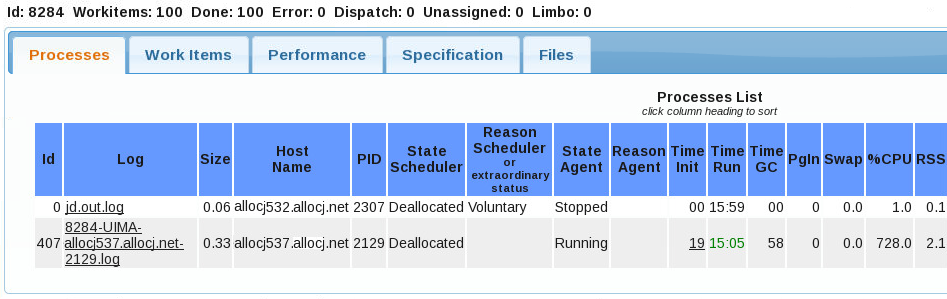
\includegraphics[width=7in]{images/BooksRaw.png}
  \caption{OpenNLP Process Measurements}
  \label{fig:OpenNLP-Process-Measurements}
\end{figure}

On the Performance tab, DUCC shows the breakdown of clock time spent in each primitive UIMA component running in the 
Job Process. See \hyperref[fig:OpenNLP-Process-Breakdown]{Figure ~\ref{fig:OpenNLP-Process-Breakdown}}.
Processing time was dominated by the Parser component at 76.7\%. The time spent compressing and writing out CASes 
was 0.5\%, and the time reading the input text files well below 0.1\%.

\begin{figure}[H]
  \centering
  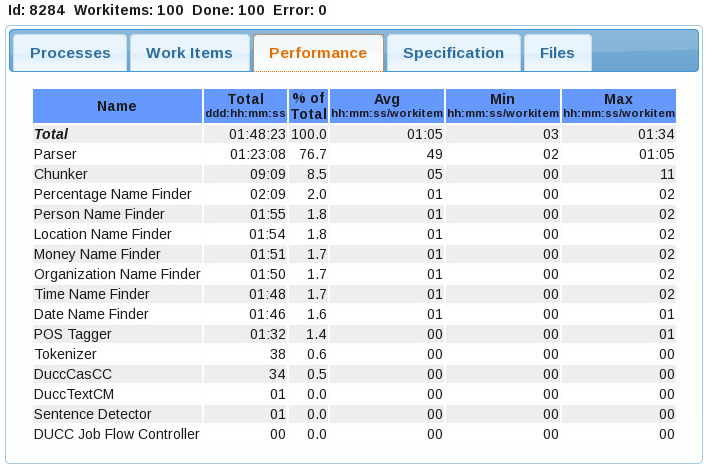
\includegraphics[width=5.5in]{images/BooksRawPerf.png}
  \caption{OpenNLP Process Breakdown}
  \label{fig:OpenNLP-Process-Breakdown}
\end{figure}


\chapter{Sample Application: CAS Input Processing}

\section{Application Function and Design}
The main purpose of this application is to demonstrate the overhead of processing a collection of CASes grouped into 
zipfiles and stored as ZIP compressed XmiCas or with UIMA compressed binary form 6 format.

	\begin{description}
    \item[Note:] This application depends on successful processing of the work in the previous chapter.
	\end{description}

\section{Configuration Parameters}
The Collection Reader for this job is the DuccJobCasCR. It has the following configuration
parameters:

\begin{description}[labelindent=0.5in,leftmargin=0.5in]
    \item[InputSpec] path to directory containing input files (named InputSpec in the hope that more options will be added).
    \item[OutputDirectory] path to directory for output files.
    \item[IgnorePreviousOutput] (optional) boolean to ignore (overwrite) previous output files.
    \item[SendToLast] (optional) boolean to route WorkItem CAS to last pipeline component. Set to true in this application.
    \item[SendToAll] (optional) boolean to route WorkItem CAS to all pipeline components. Not used in this application.
\end{description}


The CAS Consumer is the DuccCasCC and has the following configuration parameters:

\begin{description}[labelindent=0.5in,leftmargin=0.5in]
  \item[XmiCompressionLevel] (optional) compression value if using ZIP compression. Default is 7.
  \item[UseBinaryCompression] (optional) boolean to select UIMA binary CAS compression.
\end{description}

\section{Run the Job}
The job specification, DuccCasInputSpec.job, uses placeholders to reference the working directory
and various operational components located there. As run below the placeholders will be resolved
from environmental variables. 

The job is submitted from the command line with the following:
\begin{verbatim}
   MyAppDir=$PWD \
   MyInputDir=$PWD/Books.processed \ 
   MyOutputDir=$PWD/Books.followon \
   $DUCC_HOME/bin/ducc_submit -f DuccCasInputSpec.job \
   --process_deployments_max 1
\end{verbatim}

\section{Job Performance Details}
\hyperref[fig:CAS-Input-Processing]{Figure ~\ref{fig:CAS-Input-Processing}} shows the component breakdown
using binary CAS compression. Reading and deserializing took 38\% vs the 60\% spent serializing and writing.
Using 8 pipeline threads in one process the 19245 CASes output from the last application were read and 
re-written in 9 seconds.

\begin{figure}[H]
  \centering
  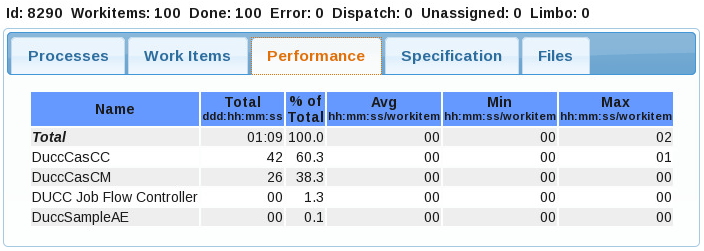
\includegraphics[width=5.5in]{images/BooksCasPerf.png}
  \caption{CAS Input Processing Performacne}
  \label{fig:CAS-Input-Processing}
\end{figure}

\section{Limiting Job Resources}
Although this 8-threaded Job Process was primarily CPU bound doing serialization work, it is possible to become I/O bound 
with enough threads banging on a shared filesystem.
DuccCasInputSpec.job demonstrates how to limit the total number of processing threads to 32 using the combination 
of process\_thread\_count=8 and process\_deployments\_max=4.

I/O vs CPU bottlenecks can be detected using the detailed performance job data reported by DUCC and comparing results
with various levels of scale out.


\part{Ducc Administrators Guide}
% 
% Licensed to the Apache Software Foundation (ASF) under one
% or more contributor license agreements.  See the NOTICE file
% distributed with this work for additional information
% regarding copyright ownership.  The ASF licenses this file
% to you under the Apache License, Version 2.0 (the
% "License"); you may not use this file except in compliance
% with the License.  You may obtain a copy of the License at
% 
%   http://www.apache.org/licenses/LICENSE-2.0
% 
% Unless required by applicable law or agreed to in writing,
% software distributed under the License is distributed on an
% "AS IS" BASIS, WITHOUT WARRANTIES OR CONDITIONS OF ANY
% KIND, either express or implied.  See the License for the
% specific language governing permissions and limitations
% under the License.
% 

% Create well-known link to this spot for HTML version
\ifpdf
\else
\HCode{<a name='DUCC_INSTALL'></a>}
\fi
\chapter{Installation, Configuration, and Verification}
% 
% Licensed to the Apache Software Foundation (ASF) under one
% or more contributor license agreements.  See the NOTICE file
% distributed with this work for additional information
% regarding copyright ownership.  The ASF licenses this file
% to you under the Apache License, Version 2.0 (the
% "License"); you may not use this file except in compliance
% with the License.  You may obtain a copy of the License at
% 
%   http://www.apache.org/licenses/LICENSE-2.0
% 
% Unless required by applicable law or agreed to in writing,
% software distributed under the License is distributed on an
% "AS IS" BASIS, WITHOUT WARRANTIES OR CONDITIONS OF ANY
% KIND, either express or implied.  See the License for the
% specific language governing permissions and limitations
% under the License.
% 
\section{Overview}

DUCC is a multi-user, multi-system distributed application.  First-time installation is performed in
two stages:

\begin{itemize}
    \item Single-user installation: This provides single-user, single-system installation for testing,
      and verification. Simple development of small applications on small systems such as laptops or
      office workstations is possible after Single-user Installation.
      
    \item Multi-user installation: This provides secure multi-user capabilities and configuration
      for multi-system clusters.
\end{itemize}

First-time users must perform single-user installation and verification on a single system.  Once
this configuration is working and verified, it is straightforward to upgrade to a multi-user
configuration.

\begin{description}
    \item[Note:] A key feature of DUCC is to run user processes in CGroups in order to guarantee
      each process always has the amount of RAM requested. Total RAM allocation to the managed process
      and its child processes that exceed requested memory will go to swap space.
      Without CGroups a process that exceeds its requested memory size by N\% is killed 
      (default N=5 in ducc.properties), and memory use by child processes is ignored.
\end{description}

DUCC is distributed as a compressed tar file.  The instructions below assume installation from one
of this distribution media.  If building from source, the build creates this file in your svn
trunk/target directory. The distribution file is in the form
\begin{verbatim}
   uima-ducc-[version]-bin.tar.gz
\end{verbatim}
where [version] is the DUCC version; for example, {\em uima-ducc-VERSION-bin.tar.gz} (where VERSION is the current DUCC version).  This document will refer to the distribution
file as the ``$<$distribution.file$>$''.

\section{Software Prerequisites}
\label{sec:install.prerequisites}
Both single and multi-user configurations have the following software pre-requisites:

\begin{itemize}
  \item A userid {\em ducc}, and group {\em ducc}.  User {\em ducc} must the the only member of group {\em ducc}.
  \item Reasonably current Linux.  DUCC has been tested on SLES 10.2, 11.1, and 11.2, and RHEL 6.3.
    
    {\em Note:} On some systems the default {\em user limits}
    for max user processes (ulimit -u) and nfiles (ulimit -n) are defined too
    low for DUCC. The shell login profile for user {\em ducc} should set the
    soft limit for max user processes to be the same as the hard limit
    (ulimit -u `ulimit -Hu`), and
    the nfiles limit raised above 1024 to at least twice the number of user
    processes running on the cluster.

  \item Sufficient swap for the expected workload.  If CGroups are configured this is
    at least 1GB and for larger systems, more.
  \item For CGroups support, libcgroup1-0.37+ on SLES and libcgroup-0.37+ on RHEL.  
  \item DUCC has been tested and run on IBM and Oracle JDK 1.6 and 1.7.
  \item Python 2.x, where 'x' is 4 or greater.  DUCC has not been tested on Python 3.x.
\end{itemize}
  
Multi-user installation has additional requirements:

\begin{itemize}
  \item All systems must have a shared filesystem (such as NFS or GPFS)  and common user space 
  \item Passwordless ssh must be installed for user {\em ducc} on all systems.
  \item Root access is required to install a small setuid-root program on each system.
\end{itemize}
  
In order to build DUCC from source the following software is also required:
\begin{itemize}
    \item A Subversion client, from \url{http://subversion.apache.org/packages.html}.  The
      svn url is \url{https://svn.apache.org/repos/asf/uima/sandbox/uima-ducc/trunk}.
    \item Apache Maven, from \url{http://maven.apache.org/index.html}
\end{itemize}

The DUCC webserver server optionally supports direct ``jconsole'' attach to DUCC job processes.  To install
this, the following is required:
\begin{itemize}
    \item Apache Ant, any reasonably current version.
\end{itemize}
    
To (optionally) build the documentation, the following is also required:
\begin{itemize}
  \item Latex, including the \emph{pdflatex} and \emph{htlatex} packages.  A good place
    to start if you need to install it is \url{https://www.tug.org/texlive/}.
\end{itemize}

More detailed one-time setup instructions for source-level builds via subversion can be found here:
\url{http://uima.apache.org/one-time-setup.html\#svn-setup}

\section{Building from Source}

To build from source, ensure you have
Subversion and Maven installed.  Extract the source from the SVN repository named above. 

Then from your extract directory into
the root directory (usually current-directory>/trunk), and run the command
\begin{verbatim}
    mvn install
\end{verbatim}
or
\begin{verbatim}
    mvn install -Pbuild-duccdocs
\end{verbatim}
if you have LaTeX insalled and wish to do the optional build of documentation.

If this is your first Maven build it may take quite a while as Maven downloads all the
open-source pre-requisites.  (The pre-requisites are stored in the Maven repository, usually
your \$HOME/.m2).

When build is complete, a tarball is placed in your current-directory/trunk/target
directory.

\section{Documentation}
\begin{sloppypar}
After single-user installation, the DUCC documentation is found (in both PDF and HTML format) in the directory 
ducc\_runtime/docs.  As well, the DUCC webserver contains a link to the full documentation on each major page.
The API is documented only via JavaDoc, distributed in the webserver's root directory 
{\tt \duccruntime/webserver/root/doc/api.}  
\end{sloppypar}

If building from source, Maven places the documentation in
\begin{itemize}
    \item {\tt trunk/uima-ducc-duccdocs/target/site} (main documentation), and 
    \item {\tt trunk/target/site/apidocs} (API Javadoc)
\end{itemize}

\section{Single-user  Installation and Verification}

Single-user installation sets up an initial, working configuration on a single system.  
Although any user ID can be used to run DUCC in single-user mode, it is recommended to create user ``ducc''
to avoid confusion. No security is established in single-user mode, and all user processes run as
the DUCC user ID.

Verification submits a very simple UIMA pipeline for execution under DUCC.  Once this is shown to be
working, one may proceed to upgrade to full installation.


\section{Minimal Hardware Requirements for single-user Installation}
\begin{itemize}
    \item One Intel-based or IBM Power-based system.  (More systems may be added during multi-user
      installation, described below.)

    \item 8GB of memory.  16GB or more is preferable for developing and testing applications beyond
      the non-trivial.  

    \item 1GB disk space to hold the DUCC runtime, system logs, and job logs.  More is
      usually needed for larger installations.  
\end{itemize}

Please note: DUCC is intended for scaling out memory-intensive UIMA applications over computing
clusters consisting of multiple nodes with large (16GB-256GB or more) memory.  The minimal
requirements are for initial test and evaluation purposes, but will not be sufficient to run actual
workloads.

\section{Single-user System Installation}
\label{subsec:install.single-user}
    \begin{enumerate}
      \item Expand the distribution file:
\begin{verbatim}
tar -zxf <distribution.file>
\end{verbatim}

        This creates a directory with a name of the form ``apache-uima-ducc-[version]''.
  
        This directory contains the full DUCC runtime which
        you may use ``in place'' but it is highly recommended that you move it
        into a standard location; for example, under ducc's HOME directory:
\begin{verbatim}
mv apache-uima-ducc-[version] /home/ducc/ducc_runtime
\end{verbatim}

        We refer to this directory, regardless of its location, as \duccruntime. For simplicity,
        some of the examples in this document assume it has been moved to /home/ducc/ducc\_runtime.

      \item Change directories into the admin sub-directory of \duccruntime: 
\begin{verbatim}
cd $DUCC_HOME/admin
\end{verbatim}

        \item Run the post-installation script: 
\begin{verbatim}
./ducc_post_install
\end{verbatim}
          If this script fails, correct any problems it identifies and run it again.

          Note that {\em ducc\_post\_install} initializes various default parameters which 
          may be changed later by the system administrator.  Therefore it usually should be
          run only during this first installation step.

        \item If you wish to install jconsole support from the webserver, make sure Apache Ant
          is installed, and run
\begin{verbatim}
./sign_jconsole_jar
\end{verbatim}
          This step may be run at any time if you wish to defer it.

   \end{enumerate}

That's it, DUCC is installed and ready to run. (If errors were displayed during ducc\_post\_install
they must be corrected before continuing.)

The post-installation script performs these tasks:
\begin{enumerate}
    \item Verifies that the correct level of Java and Python are installed and available.
    \item Creates a default nodelist, \duccruntime/resources/ducc.nodes, containing the name of the node you are installing on.
    \item Defines the ``ducc head'' node to be to node you are installing from.
    \item Sets up the default https keystore for the webserver.
    \item Installs the DUCC documentation ``ducc book'' into the DUCC webserver root.
    \item Builds and installs the C program, ``ducc\_ling'', into the default location.
    \item Ensures that the (supplied) ActiveMQ broker is runnable.
\end{enumerate}

\section{Initial System Verification}

Here we start the basic installation, submit a simple UIMA-AS job, verify that it ran, and stop
DUCC.  Once this is confirmed working DUCC is ready to use in an unsecured, single-user mode on a
single system.

To run the verification, issue these commands.
\begin{enumerate}
  \item cd \duccruntime/admin 
  \item ./check\_ducc -s
  
    Examine the output of check\_ducc.  If any errors are shown, correct the errors and rerun
    check\_ducc until there are no errors.  
  \item Finally, start ducc: ./start\_ducc -s
  \end{enumerate}
  
  Start\_ducc will first perform a number of consistency checks.
  It then starts the ActiveMQ broker, the DUCC control processes, and a single DUCC agent on the
  local node.  Note that ``single user mode'' (-s) is specified for this first start.  This inhibits
  the checks on the permissions on ducc\_ling (described \hyperref[sec:duccling]{below}).

  You will see some startup messages similar to the following:

\begin{verbatim}
ENV: Java is configured as: /share/jdk1.6/bin/java
ENV: java full version "1.6.0_14-b08"
ENV: Threading enabled: True
MEM: memory is 15 gB
ENV: system is Linux
allnodes /home/ducc/ducc_runtime/resources/ducc.nodes
Class definition file is ducc.mixed.classes
OK: Class and node definitions validated.
OK: Class configuration checked
Starting broker on ducchead.biz.org
Waiting for broker ..... 0
Waiting for broker ..... 1
ActiveMQ broker is found on configured host and port: ducchead.biz.org:61618
Starting 1 agents
********** Starting agents from file /home/ducc/ducc_runtime/resources/ducc.nodes
Starting warm
Waiting for Completion
ducchead.biz.org Starting rm
     PID 14198
ducchead.biz.org Starting pm
     PID 14223
ducchead.biz.org Starting sm
     PID 14248
ducchead.biz.org Starting or
     PID 14275
ducchead.biz.org Starting ws
     PID 14300
ducchead.biz.org
    ducc_ling OK
    DUCC Agent started PID 14325
All threads returned
\end{verbatim}

  Now open a browser and go to the DUCC webserver's url, http://$<$hostname$>$:42133 where $<$hostname$>$ is
  the name of the host where DUCC is started.  Navigate to the Reservations page via the links in
  the upper-left corner.  You should see the DUCC JobDriver reservation in state
  WaitingForResources.  In a few minutes this should change to Assigned.  (This usually takes 3-4
  minutes in the default configuration.) Now jobs can be submitted.
  
  \begin{center}     
  \cfbox{green}{The hostname and port are configurable by
  the DUCC administrator in ducc.properties}
  \end{center}
  
  To submit a job,
  \begin{enumerate}
    \item \duccruntime/bin/ducc\_submit --specification \duccruntime/examples/simple/1.job
    \end{enumerate}
    
    Open the browser in the DUCC jobs page.  You should see the job progress through a series of
    transitions: Waiting For Driver, Waiting For Services, Waiting For Resources, Initializing, and
    finally, Running.  You'll see the number of work items submitted (15) and the number of work
    items completed grow from 0 to 15.  Finally, the job will move into Completing and then
    Completed..

    Since this example does not specify a log directory DUCC will create a log directory in your HOME directory under 
\begin{verbatim}
$HOME/ducc/logs/job-id
\end{verbatim}

    In this directory, you will find a log for the sample job's JobDriver (JD), JobProcess (JP), and
    a number of other files relating to the job.

    This is a good time to explore the DUCC web pages.  Notice that the job id is a link to a set of
    pages with details about the execution of the job.

    Notice also, in the upper-right corner is a link to the full DUCC documentation, the ``DuccBook''.

    Finally, stop DUCC:
    \begin{enumerate}
      \item cd \duccruntime/admin
      \item./stop\_ducc -a
      \end{enumerate}
      
      Once the system is verified and the sample job completes correctly, proceed to Multi-User
      Installation and Verification to set up multiple-user support and optionally, multi-node
      operation.

\section{Multi-User Installation and Verification}
  
    Multi-user installation consists of these steps over and above single-user installation:
    \begin{enumerate}
        \item Install and configure the setuid-root program, ducc\_ling.  This small program allows DUCC
          jobs to be run as the submitting user rather than user ducc.

        \item Optionally install and configure CGroups.

        \item Optionally update the configuration to include additional nodes.
     \end{enumerate}

     Multi-user installation has these pre-requisites (DUCC will not work on multiple nodes
     unless these steps are taken):
     \begin{itemize}

         \item All systems in the DUCC cluster must have a shared filesystem and shared user space (user
           directories are shared over NFS or an equivalent networked file system, across the systems, and
           user ids and credentials are the same).

         \item Passwordless ssh must be installed for user ducc on all systems. Users do NOT require
           ssh access to the DUCC nodes.
           
         \item Root access is (briefly) required to install a small setuid-root program on each system.
      \end{itemize}

\section{Ducc\_ling Installation}
\label{sec:duccling}
    Before proceeding with this step, please note: 
    \begin{itemize}
        \item This step is required ONLY to install multi-user capabilities.
        \item The sequence operations consisting of {\em chown} and {\em chmod} MUST be performed
          in the exact order given below.  If the {\em chmod} operation is performed before
          the {\em chown} operation, Linux will regress the permissions granted by {\em chmod} 
          and ducc\_ling will be incorrectly installed.
    \end{itemize}

    ducc\_ling is a setuid-root program whose function is to execute user tasks under the identity of
    the user.  This must be installed correctly; incorrect installation can prevent jobs from running as
    their submitters, and in the worse case, can introduce security problems into the system.

    ducc\_ling must be installed on LOCAL disk on every system in the DUCC cluster, to avoid
    shared-filesystem access to it.  The path to ducc\_ling must be the same on each system.  For
    example, one could install it to /local/ducc/bin on local disk on every system.

    To install ducc\_ling (these instructions assume it is installed into /local/ducc/bin):
    As ducc, ensure ducc\_ling is built correctly for your architecture:
    \begin{enumerate}
        \item cd \duccruntime/duccling/src
        \item make clean all
     \end{enumerate}
        
     Now, as root, move ducc\_ling to a secure location and grant authorization to run tasks under
     different users' identities:
     \begin{enumerate}
         \item mkdir /local/ducc
         \item mkdir /local/ducc/bin
         \item chown ducc.ducc /local/ducc
         \item chown ducc.ducc /local/ducc/bin
         \item chmod 700 /local/ducc
         \item chmod 700 /local/ducc/bin
         \item cp \duccruntime/duccling/src/ducc\_ling /local/ducc/bin
         \item chown root.ducc /local/ducc/bin/ducc\_ling
         \item chmod 4750 /local/ducc/bin/ducc\_ling
      \end{enumerate}
         
      Finally, update the configuration to use this ducc\_ling instead of the default ducc\_ling:
      \begin{enumerate}
        \item Edit \duccruntime/resources/ducc.properties and change this line:         
\begin{verbatim}
 ducc.agent.launcher.ducc_spawn_path=${DUCC_HOME}/admin/ducc_ling
\end{verbatim}
          to this line (Using the actual location of the updated ducc\_ling, if different from /local/ducc/bin):
\begin{verbatim}
ducc.agent.launcher.ducc_spawn_path=/local/ducc/bin/ducc_ling
\end{verbatim}
        \end{enumerate}


        What these steps do:
      \begin{enumerate}
          \item The first two step compile ducc\_ling for your current machine architecture and
            operating system level.
          \item The next two steps (mkdir) create directory /local/ducc/bin
          \item The next two steps (chown) set ownership of /local/ducc and /local/ducc/bin to user ducc,
            group ducc
          \item The next two steps (chmod) set permissions for /local/ducc and /local/ducc/bin so only user
            ducc may access the contents of these directories
          \item The copy stop copies the ducc\_ling program created in initial installation into /local/ducc/bin
          \item The next step (chown) sets ownership of /local/ducc/bin/ducc\_ling to root, and
            group ownership to ducc.
          \item The next step (chmod) stablishes the {\em setuid} bit, which allows user ducc to execute ducc\_ling
            with root privileges.
          \item Finally, ducc.properties is updated to point to the new, privileged ducc\_ling.
       \end{enumerate}
          
       If these steps are correctly performed, ONLY user {\em ducc} may use the ducc\_ling program in
       a privileged way. Ducc\_ling contains checks to prevent even user {\em root} from using it for
       privileged operations.

       Ducc\_ling contains the following functions, which the security-conscious may verify by examining
       the source in \duccruntime/duccling.  All sensitive operations are performed only AFTER switching
       userids, to prevent unauthorized root access to the system.
       \begin{itemize}
         \item Changes it's real and effective userid to that of the user invoking the job.
         \item Optionally redirects its stdout and stderr to the DUCC log for the current job.
         \item Optionally redirects its stdio to a port set by the CLI, when a job is submitted.
         \item ``Nice''s itself to a ``worse'' priority than the default, to reduce the chances
           that a runaway DUCC job could monopolize a system.
         \item Optionally sets user limits.
         \item Prints the effective limits for a job to both the user's log, and the DUCC agent's log.
         \item Changes to the user's working directory, as specified by the job.
         \item Optionally establishes LD\_LIBRARY\_PATH 
           for the job from the environment variable
\begin{verbatim}
        DUCC_LD_LIBRARY_PATH
\end{verbatim}
           if set in the DUCC job specification. (Secure Linux systems will
           prevent LD\_LIBRARY\_PATH 
           from being set by a program with root authority, so this is
           done AFTER changing userids).

       \end{itemize}

\section{CGroups Installation and Configuration}
    The steps in this task must be done as user root and user ducc.

    To install and configure CGroups for DUCC:
    \begin{enumerate}
       \item Install the appropriate \hyperref[sec:install.prerequisites]{libcgroup package} at level 0.37
         or above.

       \item Configure /etc/cgconfig.conf as follows:
\begin{verbatim}
   # Mount cgroups
   mount {
      memory = /cgroup;
   }
   # Define cgroup ducc and setup permissions
   group ducc {
    perm {
        task {
           uid = ducc;
        }
        admin {
           uid = ducc;
        }
    }
    memory {}
   }
\end{verbatim}
       \item Start the cgconfig service:
\begin{verbatim}
   service cgconfig start
\end{verbatim}
         
       \item Verify cgconfig service is running by the existence of directory: 
\begin{verbatim}
   /cgroups/ducc
\end{verbatim}

       \item Some versions of libcgroup are buggy. As user ducc, verify that the following command executes with no error:
\begin{verbatim}
   cgcreate -t ducc -a ducc -g memory:ducc/test-cgroups
\end{verbatim}
         
       \item Configure the cgconfig service to start on reboot:
\begin{verbatim}
   chkconfig cgconfig on
\end{verbatim}

       \item Update \hyperref[itm:props-agent.cgroups.enable]{ducc.properties} to enable CGroups.
         Note that if CGroups is not installed, the DUCC Agent will detect this and not attempt to
         use the feature.  It is completely safe to enable CGroups in {\em ducc.properties} on
         machines where it is not installed.
    \end{enumerate}

\section{Set up the full nodelists}
   To add additional nodes to the ducc cluster, DUCC needs to know what nodes to start its Agent
   processes on.  These nodes are listed in the file
\begin{verbatim}
$DUCC_HOME/resources/ducc.nodes.  
\end{verbatim}
   
   During initial installation, this file was initialized with the node DUCC is installed on.
   Additional nodes may be added to the file using a text editor to increase the size of the DUCC
   cluster.
 
\section{Full DUCC Verification}

This is identical to initial verification, with the one difference that the job ``1.job'' should be
submitted as any user other than ducc.  Watch the webserver and check that the job executes
under the correct identity.  Once this completes, DUCC is installed and verified.
 
\section{Enable DUCC webserver login}

    This step is optional.  As shipped, the webserver is disabled for
    logins.  This can be seen by hovering over the Login text located in the
    upper right of most webserver pages: 
\begin{verbatim}
System is configured to disallow logins
\end{verbatim}

    To enable logins, a Java-based authenticator must be plugged-in and the
    login feature must be enabled in the ducc.properties file by the DUCC
    administrator.  Also, ducc\_ling should be properly deployed (see 
    Ducc\_ling Installation section above).
    
    A beta version of a Linux-based authentication plug-in is shipped with DUCC.
    It can be found in the source tree:
\begin{verbatim}
org.apache.uima.ducc.ws.authentication.LinuxAuthenticationManager
\end{verbatim}

    The Linux-based authentication plug-in will attempt to validate webserver
    login requests by appealing to the host OS.  The user who wishes to
    login provides a userid and password to the webserver via https, which
    in-turn are handed-off to the OS for a success/failure reply.
    
    To have the webserver employ the beta Linux-based authentication plug-in,
    the DUCC administrator should perform the following as user ducc:
\begin{verbatim}    
1. edit ducc.properties
2. locate: ducc.ws.login.enabled = false
3. modify: ducc.ws.login.enabled = true
4. save
\end{verbatim}

    Note: The beta Linux-based authentication plug-in has limited testing.
    In particular, it was tested using:
\begin{verbatim}
Red Hat Enterprise Linux Workstation release 6.4 (Santiago)
\end{verbatim}    
    
    Alternatively, you can provide your own authentication plug-in.  To do so:
\begin{verbatim}    
1. author a Java class that implements 
   org.apache.uima.ducc.common.authentication.IAuthenticationManager
2. create a jar file comprising your authentication class
3. put the jar file in a location accessible by the DUCC webserver, such as 
    $DUCC_HOME/lib/authentication
4. put any authentication dependency jar files there as well
5. edit ducc.properties
6. add the following:
   ducc.local.jars = authentication/*
   ducc.authentication.implementer=<your.authenticator.class.Name>
7. locate: ducc.ws.login.enabled = false
8. modify: ducc.ws.login.enabled = true
9. save   
\end{verbatim}    



% Create well-known link to this spot for HTML version
\ifpdf
\else
\HCode{<a name='DUCC_ADMIN'></a>}
\fi
\chapter{Administration}

%% These should all be sections
% 
% Licensed to the Apache Software Foundation (ASF) under one
% or more contributor license agreements.  See the NOTICE file
% distributed with this work for additional information
% regarding copyright ownership.  The ASF licenses this file
% to you under the Apache License, Version 2.0 (the
% "License"); you may not use this file except in compliance
% with the License.  You may obtain a copy of the License at
% 
%   http://www.apache.org/licenses/LICENSE-2.0
% 
% Unless required by applicable law or agreed to in writing,
% software distributed under the License is distributed on an
% "AS IS" BASIS, WITHOUT WARRANTIES OR CONDITIONS OF ANY
% KIND, either express or implied.  See the License for the
% specific language governing permissions and limitations
% under the License.
% 
\section{WebServer Authentication}
\label{sec:WebServer Authentication}

    By default, DUCC is configured such that there is effectively no
    authentication enforcement by the WebServer. No password entry is permitted
    on the Login panel and any userid specified is accepted whether it exists or
    not.
    
    To enable your own authentication measures, you should perform the following
    steps:
    
    \begin{enumerate}
      \item Author an authentication manager Java class implementing interface
      \begin{verbatim}
org.apache.uima.ducc.common.authentication.IAuthenticationManager
      \end{verbatim}
      \item Create an authentication jar file comprising the
      authentication manager Java class
      \item Install your authentication jar file and any dependency jar files
      into your DUCC's lib folder
      \item Update your ducc.properties file with authentication class name
      and jar file name(s) information
      \item Create a ducc.administrators file
      \end{enumerate}
      
    Note: When a user clicks on the WebServer Login link, the login dialog is
    shown. On that dialog panel is shown the \mbox{authenticator: {\em
    version}}, which is supplied by your authentication manager implementation's {\em
    \mbox{getVersion()}} method. Also shown are boxes for userid and password
    entry. If your authentication manager implemenation's {\em \mbox{isPasswordChecked()}}
    method returns true then the password box will accept input, otherwise it will be
    disabled.
    
\subsection{Example Implementation}
    
    Shown below is an example implementation which can be used as a template
    for coding protection by means of interfacing with your site's security
    measures.
    
    In this example, the SiteSecurity Java class is presumed to be existing
    and available code at your installation.
    
    \begin{verbatim}
package org.apache.uima.ducc.example.authentication.module;

import org.apache.uima.ducc.common.authentication.AuthenticationResult;
import org.apache.uima.ducc.common.authentication.IAuthenticationManager;
import org.apache.uima.ducc.common.authentication.IAuthenticationResult;
import org.apache.uima.ducc.example.authentication.site.SiteSecurity;

public class AuthenticationManager implements IAuthenticationManager {

    private final String version = "example 1.0";
    
    @Override
    public String getVersion() {
        return version;
    }

    @Override
    public boolean isPasswordChecked() {
        return true;
    }

    @Override
    public IAuthenticationResult isAuthenticate(String userid, String domain,
            String password) {
        IAuthenticationResult authenticationResult = new AuthenticationResult();
        authenticationResult.setFailure();
        try {
            if(SiteSecurity.isAuthenticUser(userid, domain, password)) {
                authenticationResult.setSuccess();
            }
        }
        catch(Exception e) {
            //TODO
        }
        return authenticationResult;
    }

    @Override
    public IAuthenticationResult isGroupMember(String userid, String domain,
            Role role) {
        IAuthenticationResult authenticationResult = new AuthenticationResult();
        authenticationResult.setFailure();
        try {
            if(SiteSecurity.isAuthenticRole(userid, domain, role.toString())) {
                authenticationResult.setSuccess();
            }
        }
        catch(Exception e) {
            //TODO
        }
        return authenticationResult;
    }

}
    \end{verbatim}
        
\subsection{IAuthenticationManager}
       
    Shown below is the interface which must be implemented by your
    authentication manager.
    
    \begin{verbatim}
package org.apache.uima.ducc.common.authentication;

public interface IAuthenticationManager {
    
    /**
     * This method is expected to return AuthenticationManager implementation version 
     * information.  It is nominally displayed by the DUCC webserver on the Login/Logout 
     * pages.
     * 
     * Example return value: Acme Authenticator 1.0
     * 
     * @return The version of the AuthenticationManager implementation.
     */
    public String getVersion();
    
    /**
     * This method is expected to return password checking information.  
     * It is nominally employed by the DUCC webserver to enable/disable
     *  password input area on the Login/Logout pages.
     * 
     * @return True if the AuthenticationManager implementation checks passwords; 
     * false otherwise.
     */
    public boolean isPasswordChecked();
    
    /**
     * This method is expected to perform authentication.
     * It is nominally employed by the DUCC webserver for submitted Login pages.
     * 
     * @param userid
     * @param domain
     * @param password
     * @return True if authentic userid+domain+password; false otherwise.
     */
    public IAuthenticationResult isAuthenticate(String userid, String domain, String password);
    
    /**
     * This method is expected to perform role validation.
     * It is nominally employed by the DUCC webserver for submitted Login pages.
     * 
     * @param userid
     * @param domain
     * @param role
     * @return True if authentic userid+domain+role; false otherwise.
     */
    public IAuthenticationResult isGroupMember(String userid, String domain, Role role);
    
    /**
     * The supported Roles
     */
    public enum Role {
        User,
        Admin
    }
}
    \end{verbatim}


\subsection{IAuthenticationResult}
    
    Shown below is the interface which must be returned by the required
    authentication methods in your authentication manager.
    
    \begin{verbatim}
package org.apache.uima.ducc.common.authentication;
    
public interface IAuthenticationResult {
    public void setSuccess();
    public void setFailure();
    public boolean isSuccess();
    public boolean isFailure();
    public void setCode(int code);
    public int getCode();
    public void setReason(String reason);
    public String getReason();
    public void setException(Exception exception);
    public Exception getException();
}
    \end{verbatim}
    
\subsection{Example ANT script to build jar}
    
    Shown below is an example ANT script to build a ducc-authenticator.jar file.
    The resulting jar file should be placed user DUCC's lib directory along with
    any dependency jars, and defined in ducc.properties file.
    
    \begin{verbatim}
<project name="uima-ducc-examples" default="build" basedir=".">
    
    <property name="TGT-LIB"                value="${basedir}/lib" />
    <property name="TGT-DUCC-AUTH-JAR"      value="${TGT-LIB}/ducc-authenticator.jar" />
    
    <target name="build" depends="clean, jar" />
    
    <target name="clean">
        <delete file="${TGT-DUCC-AUTH-JAR}" />
    </target>
    
    <target name="jar">
        <mkdir dir="${TGT-LIB}" />
        <jar destfile="${TGT-DUCC-AUTH-JAR}" basedir="${basedir}/target/classes/org/apache/uima/ducc/example/authentication/module"/>
    </target>
    
</project>
    \end{verbatim}
    
\subsection{Example ducc.properties entries}
    
    Shown here is a snippet of the ducc.properties file defining the class to be
    used for authentication and the administrator created folder
    {\em site-security}, which should contain the ducc-authenticator.jar you
    built plus any jar files upon which it depends.
    
    Note: the {\em site-security} directory must be located within DUCC's lib
    directory.
    
    \begin{verbatim}
# The class that performs authentication (for the WebServer)
ducc.authentication.implementer = org.apache.uima.ducc.example.authentication.module.AuthenticationManager

# Site specific jars: include all jars in directory site-security
ducc.local.jars = site-security/*
    \end{verbatim}
    
\subsection{Example ducc.administrators}
    
    Example contents of ducc.administrators file located within DUCC's resources
    directory. Only userids listed here can assume the Administrator role when 
    performing operations via the WebServer.
    
    \begin{verbatim}
jdoe
fred
hal9000
    \end{verbatim}


  

% 
% Licensed to the Apache Software Foundation (ASF) under one
% or more contributor license agreements.  See the NOTICE file
% distributed with this work for additional information
% regarding copyright ownership.  The ASF licenses this file
% to you under the Apache License, Version 2.0 (the
% "License"); you may not use this file except in compliance
% with the License.  You may obtain a copy of the License at
% 
%   http://www.apache.org/licenses/LICENSE-2.0
% 
% Unless required by applicable law or agreed to in writing,
% software distributed under the License is distributed on an
% "AS IS" BASIS, WITHOUT WARRANTIES OR CONDITIONS OF ANY
% KIND, either express or implied.  See the License for the
% specific language governing permissions and limitations
% under the License.
% 
\section{ducc.properties}
\label{sec:ducc.properties}
    The primary configuration file is called ducc.properties and always resides in the directory
    ducc\_runtime/resources.

    Some of the properties in ducc.properties are intended as the "glue" that brings the various 
    DUCC components together and lets then run as a coherent whole. These types of properties should 
    be modified only by developers of DUCC itself. In the description below these properties are 
    classified as "Private". 

    Some of the properties are tuning parameters: timeouts, heartbeat intervals, and so on. These
    may be modified by DUCC administrators, but only after experience is gained with DUCC, and only
    to solve specific performance problems. The default tuning parameters have been chosen by the
    DUCC system developers to provide "best" operation under most reasonable situations. In the
    description below these properties are classified as "Tuning".

    Some of the properties describe the local cluster configuration: the location of the ActiveMQ
    broker, the location of the Java JRE, port numbers, etc. These should be modified by the DUCC
    administrators to configure DUCC to each individual installation. In the description below these
    properties are classified as "Local".
    
\subsection{General DUCC Properties}
    \begin{description}

       \item[ducc.authentication.implementer] \hfill \\
         This specifies the class used for WebServer session authentication.  If unconfigured,
         the Web Server enforces no authentication.
         \begin{description}
           \item[Default] org.apache.uima.ducc.common.authentication.LinuxAuthenticationManager
           \item[Type] Local
         \end{description}

       \item[ducc.admin.endpoint] \hfill \\
         This is the JMS endpoint name used for DUCC administration messages. 
         \begin{description}
           \item[Default] ducc.admin.channel 
           \item[Type] Private 
         \end{description}

       \item[ducc.admin.endpoint.type] \hfill \\
         This is the JMS message type used for DUCC administration requests. If changed DUCC 
         admin may not work. 
         \begin{description}
           \item[Default] topic 
           \item[Type] Private
         \end{description} 
           
       \item[ducc.broker.automanage] \hfill \\
         If set to ``true'', DUCC will start and stop the ActiveMQ broker as part of its normal start/stop
         scripting.  
         \begin{description}
           \item[Default] true
           \item[Type] Tuning
         \end{description} 

       \item[ducc.broker.home] \hfill \\
         For DUCC auto-managed brokers only, this names the location where ActiveMQ is installed
         installed.  

         Note that the DUCC installation includes a default ActiveMQ.
         \begin{description}
           \item[Default] \duccruntime/activemq 
           \item[Type] Tuning
         \end{description} 
           
       \item[ducc.broker.memory.options] \hfill \\
         For DUCC auto-managed brokers only, this names the ActiveMQ configuration file.  The configuration
         file is assumed to reside in the directory specified by {\em ducc.broker.home}, so the path must be relative
         to that location.
         \begin{description}
           \item[Default] conf/activemq-ducc.xml
           \item[Type] Tuning
         \end{description} 
           
           
       \item[ducc.broker.decoration] \hfill \\
         The property is used by the DUCC Job Driver processes to modify the ActiveMQ broker URL
         when connecting to the Job Processes.

         The supplied default is used to disable broker connection timeouts.  From the ActiveMQ
         documentation: "The maximum inactivity duration (before which the socket is considered
         dead) in milliseconds. On some platforms it can take a long time for a socket to appear to
         die, so we allow the broker to kill connections if they are inactive for a period of
         time. Use by some transports to enable a keep alive heart beat feature. Set to a value
         less-than-or-equal0 to disable inactivity monitoring. Declare the wire protocol used to
         communicate with ActiveMQ."
         
         This decoration is used to keep the broker connection alive while a JVM is in a
         long garbage collection. The applications that DUCC is designed to support can
         spend significant time in garbage collection, which can cause spurious timeouts. By
         default the DUCC configuration disables the timeout by setting it to 0.       

         \begin{description}
           \item[Default] wireFormat.maxInactivityDuration=0 
           \item[Type] Local 
         \end{description}

       \item[ducc.broker.hostname] \hfill \\
         This declares the node where the ActiveMQ broker resides. It MUST be updated to 
         the actual node where the broker is running as part of DUCC installation. The default value 
         will not work.          
         \begin{description}               
           \item[Default] \$\{ducc.head\}.  The default is defined in the ducc property, {\em ducc.head}.
             If you want to run the ActiveMQ broker on the ``ducc head'', this parameter need not
             be changed.
           \item[Type] Local 
         \end{description}

       \item[ducc.broker.jmx.port] \hfill \\
         This is the port used to make JMX connections to the broker.  This should only
         be changed by administrators familiar with ActiveMQ configuration.         
         \begin{description}         
           \item[Default] 1100                      
           \item[Type] Local 
         \end{description}

       \item[ducc.broker.memory.options] \hfill \\
         For DUCC auto-managed brokers only, this sets the {\tt -Xmx} heap size for the broker.
         \begin{description}
           \item[Default] -Xmx2G
           \item[Type] Tuning
         \end{description} 
           

       \item[ducc.broker.name] \hfill \\
         This is the internal name of the broker, used to locate Broker's MBean in JMX Registry. 
         It is NOT related to any node name. When using the ActiveMQ distribution supplied with 
         DUCC it should always be set to "localhost".  The default should be changed only by
         administrators familiar with ActiveMQ configuration.
         \begin{description}
           \item[Default] localhost 
           \item[Type] Local              
         \end{description}


       \item[ducc.broker.port] \hfill \\
         This declares the port on which the ActiveMQ broker is listening for
         messages. It MAY be updated as part of DUCC installation. ActiveMQ ships with port
         61616 as the default port, and DUCC uses that default.         
         \begin{description}
           \item[Default] 61617              
           \item[Type] Local 
         \end{description}
             

       \item[ducc.broker.protocol] \hfill \\
         Declare the wire protocol used to communicate with ActiveMQ. 
         \begin{description}
           \item[Default] tcp 
           \item[Type] Private 
         \end{description}


       \item[ducc.broker.server.url.decoration] \hfill \\
         For DUCC auto-managed brokers only, this configures ActiveMQ Server url decoration.
         
         \begin{description}
           \item[Default] transport.soWriteTimeout=45000
           \item[Type] Tuning
         \end{description} 

       \item[ducc.cli.httpclient.sotimeout] \hfill \\
         This is the timeout used by the CLI to communicate with DUCC, in milliseconds. If no 
         response is heard within this time, the request times out and is aborted. When set to 0 (the 
         default), the request never times out. 
         \begin{description}
           \item[Default] 0 
           \item[Type] Tuning 
          \end{description}

       \item[ducc.cluster.name] \hfill \\
         This is a string used in the Web Server banner to identify the local cluster. It is used
         for informational purposes only and may be set to anything desired.
         \begin{description}
           \item[Default] Apache UIMA-DUCC
           \item[Type] Local 
         \end{description}
          
       \item[ducc.head] \hfill \\
         This property declares the node where the DUCC adminstrative processes run (Orchestrator,
         Resource Manager, Process Manager, Service Manager).  This property is required and MUST be
         configured in new installation.  The installation script
         \hyperref[subsec:install.single-user]{ducc\_post\_install} initializes this property to the
         node the script is executed on.
         \begin{description}
           \item[Default] There is no default, this must be configured during system installation.
           \item[Type] Local 
         \end{description}

       \item[ducc.jms.provider] \hfill \\
         Declare the type of middleware providing the JMS service used by DUCC.
         \begin{description}
           \item[Default] activemq 
           \item[Type]Private 
         \end{description}

       \item[ducc.jmx.port] \hfill \\
         Every process started by DUCC has JMX enabled by default. When more than one process 
         runs on the same machine this can cause port conflicts. The property "ducc.jmx.port" is 
         used as the base port for JMX. If the port is busy, it is incremented internally until a free 
         port is found. 
         
         The web server's \hyperref[sec:system-details.daemons]{"System $->$ Daemons"} tab is used
         to find the JMX URL that gets assigned to each of the DUCC management processes. The web
         server's \hyperref[sec:ws-job-details]{Job details} page for each job is used to find the
         JMX URL that is assigned to each JP.
         
         \begin{description}
           \item[Default] 2099 
           \item[Type] Private 
         \end{description}

       \item[ducc.jvm] \hfill \\
         This specifies the full path to the JVM to be used by the DUCC processes. This MUST be
         configured.  The installation script
         \hyperref[subsec:install.single-user]{ducc\_post\_install} initializes this property to 
         full path to ``java'' in the installer's environment.  (If the ``java'' command cannot
         be found, ducc\_post\_install exits with error.)
         \begin{description}
           \item[Default] None.  Must be configured during installation.
           \item[Type] Local 
         \end{description}

       \item[ducc.node.min.swap.threshold] \hfill \\
         Specify a minimum amount of free swap space available on a node.
         If an agent detects free swap space dipping below the value defined
         below, it will find the fattest (in terms of memory) process in its
         inventory and kill it. The value of the parameter below is expressed
         in Megabytes.

         If set to 0, the threshold is disabled.
         \begin{description}
           \item[Default] 0
           \item[Type] Tuning
         \end{description}


       \item[ducc.agent.jvm.args] \hfill \\
         This specifies the list of arguments passed to the JVM when spawning the Agent. 
         \begin{description}           
           \item[Default] -Xmx100M 
           \item[Type] Tuning 
         \end{description}


       \item[ducc.driver.jvm.args] \hfill \\
         If enabled, the arguments here are automatically added to the JVM arguments specified for 
         the Job Driver process. 

         Note: if the user-supplied JVM arguments contain a -Xmx entry then 
         any -Xmx value specified here will be ignored.
         \begin{description}
           \item[Default] (unconfigured) 
           \item[Type] Local 
         \end{description}

       \item[ducc.orchestrator.jvm.args] \hfill \\
         This specifies the list of arguments passed to the JVM when spawning the Orchestrator. 
         \begin{description}
           \item[Default] -Xmx1G 
           \item[Type] Tuning 
         \end{description}


       \item[ducc.pm.jvm.args] \hfill \\
         This specifies the list of arguments passed to the JVM when spawning the Process Manager. 
         \begin{description}
           \item[Default] -Xmx1G 
           \item[Type] Tuning 
         \end{description}

       \item[ducc.process.jvm.args] \hfill \\
         If enabled, the arguments here are added by DUCC to the JVM arguments in the user's job 
         processes. 
         \begin{description}
           \item[Default] (unconfigured) 
           \item[Type] Private 
         \end{description}
                   
       \item[ducc.rm.jvm.args] \hfill \\
         This specifies the list of arguments passed to the JVM when spawning the Resource 
         Manager. 
         \begin{description}           
           \item[Default] -Xmx1G 
           \item[Type] Tuning 
         \end{description}

       \item[ducc.sm.jvm.args] \hfill \\
         This specifies the list of arguments passed to the JVM when spawning the Service Manager. 
         \begin{description}
           \item[Default] -Xmx1G 
           \item[Type] Tuning 
         \end{description}

       \item[ducc.ws.jvm.args] \hfill \\
         specifies the list of arguments passed to the JVM when spawning the
         Webserver.
         \begin{description}
           \item[Default] -Xmx8G 
           \item[Type] Tuning 
         \end{description}

       \item[ducc.locale.language] \hfill \\
         Establish the language for national language support of messages. Currently only "en" is 
         supported. 
         \begin{description}
           \item[Default] en 
           \item[Type] Private 
         \end{description}
           
       \item[ducc.locale.country] \hfill \\
         Establish the country for National Language Support of messages. Currently only "us" is 
         supported. 
         \begin{description}
           \item[Default] us 
           \item[Type] Private 
         \end{description}


       \item[ducc.runmode] \hfill \\
         When set to "Test" this property bypasses userid and authentication checks. It is intended 
         for use ONLY by DUCC developers. It allows developers of DUCC to simulate a multiuser 
         environment without the need for root privileges. 
         
         Note: WARNING! Enabling this feature in a production DUCC system is a potentially serious
         security breach. It should only be set by DUCC developers running with an un-privileged
         ducc\_ling.
         \begin{description}
           \item[Default] Unconfigured. When unconfigured, test mode is DISABLED.
           \item[Type] Local 
         \end{description}


        \item[ducc.signature.required] \hfill \\
          When set, the CLI signs each request so the Orchestrator can be sure the requestor is 
          actually who he claims to be. 
          \begin{description}            
            \item[Default] on             
            \item[Type] Tuning 
          \end{description}


       \item[ducc.threads.limit] \hfill \\
         This enforces a maximum number of pipeline threads per job, over all its processes. No 
         job will have more active work-items than this dispatched. This limit is disabled by default. 

         The value represents the size of the underlying CAS pool in the Job Driver and therefore
         is related to the size of the Job Driver heap and the real memory consumed by JD.  If
         the JD is consuming too much memory, try setting or reducing this value.
         
         \begin{description}
           \item[Default] (unconfigured) 
           \item[Type] Local 
         \end{description}

       \item[ducc.environment.propagated] \hfill \\
         This specifies the environmental variables whose values will be merged with the
         user-specified environment option on job, process and service submissions.  A typical setting
         might be: USER HOME LANG

         \begin{description}
           \item[Default] (unconfigured) 
           \item[Type] Local 
         \end{description}
                                                                        
      \end{description}  
        

\subsection{Web Server Properties}

    \begin{description}
        \item[ducc.ws.configuration.class] \hfill \\
          The name of the pluggable java class used to implement the Web Server. 
          \begin{description}
            \item[Default Value] org.apache.uima.ducc.ws.config.WebServerConfiguration 
            \item[Type] Private 
          \end{description}
        
        \item[ducc.ws.node] \hfill \\
          This is the name of the node the web server is started on. If not specified, the web server is 
          started on {\tt \$\{ducc\.head\}}.
          \begin{description}
            \item[Default Value] (unconfigured) 
            \item[Type] Local 
          \end{description}
            

        \item[ducc.ws.ipaddress] \hfill \\
          In multi-homed systems it may be necessary to specify to which of the multiple addresses 
          the Web Server listens for requests. This property is an IP address that specifies to which 
          address the Web Server listens. 
          \begin{description}
            \item[Default Value] (unconfigured) 
            \item[Type] Local 
          \end{description}
              
        \item[ducc.ws.port] \hfill \\
          This is the port on which the DUCC Web Server listens for requests. 
          \begin{description}
            \item[Default Value] 42133 
            \item[Type] Local 
          \end{description}

        \item[ducc.ws.port.ssl] \hfill \\
          This is the port that the Web Server uses for SSL requests (such as authentication). 
          \begin{description}
            \item[Default Value] 42155 
            \item[Type] Local 
          \end{description}

        \item[ducc.ws.port.ssl.pw] \hfill \\
          This is the password used to generate the Web Server's keystore used for HTTPS requests.  Usually
          this keystore is created at initial installation time using \hyperref[subsec:install.single-user]{ducc\_post\_install.}
          \begin{description}
            \item[Default Value] quackquack 
            \item[Type] Local
          \end{description}
                    
        \item[ducc.ws.session.minutes] \hfill \\
          Once authenticated, this property determines the lifetime of the authenticated session to the 
          Web Server. 
          \begin{description}
            \item[Default Value] 60 
            \item[Type] Tuning
          \end{description}

        \item[ducc.ws.max.history.entries] \hfill \\
          DUCC maintains a history of all jobs.  The state of jobs, both old and current are shown
          in the Webserver's Jobs Page.  To avoid overloading this page and the Web Server, the maximum
          number of entries that can be shown is regulated by this parameter.
          \begin{description}
            \item[Default Value] 4096
            \item[Type] Tuning
          \end{description}

        \item[ducc.ws.login.enabled] \hfill \\
          If true, users are allowed to login to Webserver.  If false, users are
          not allowed to login to Webserver.  Shipped value set to false. 
          However, default value if property not specified is true.
          \begin{description}
            \item[Default Value] true
            \item[Type] Tuning
          \end{description}

        \item[ducc.ws.automatic.cancel.minutes] \hfill \ Optionally configure the webserver job
          automatic cancel timeout. To disable this feature specify 0.  This is employed when a user
          specifies {\em$--$wait\_for\_completion} flag on job submission, in which case the job
          monitor program must visit 
\begin{verbatim}
   http://<host>:<port>/ducc-servlet/proxy-job-status?id=<job-id>
\end{verbatim}
          within this expiry time.  Otherwise the job will be automatically canceled.

          This provides a safeguard against runaway jobs or managed reservations, if the
          submitter gets disconnected from DUCC in some way.

          If the feature is disabled by specifing ``0'', no work is canceled even if the
          monitor itself disappears.

          \begin{description}
            \item[Default Value] 10
            \item[Type] Tuning
          \end{description}

        \item[ducc.ws.jsp.compilation.directory] \hfill \\
          This specifies the temporary used by the Web Server's JSP engine to compile its JSPs.
          \begin{description}
            \item[Default Value] /tmp/ducc/jsp
            \item[Type] Tuning
          \end{description}

      \end{description}  
            
    
\subsection{Job Driver Properties}
    \begin{description}
        \item[ducc.jd.configuration.class] \hfill \\
          The name of the pluggable java class used to implement the Job Driver. 
          \begin{description}
            \item[Default Value] org.apache.uima.ducc.jd.config.JobDriverConfiguration 
            \item[Type] Private 
          \end{description}
          
        \item[ducc.jd.state.update.endpoint] \hfill \\
          This is the JMS endpoint name by the Job Driver to send state to the Orchestrator. 
          \begin{description}
            \item[Default Value] ducc.jd.state               
            \item[Type] Private 
          \end{description}
            

        \item[ducc.jd.state.update.endpoint.type] \hfill \\
          This is the JMS message type used to send state to the Orchestrator. 
          \begin{description}            
            \item[Default Value] topic 
            \item[Type] Private 
          \end{description}
          

        \item[ducc.jd.state.publish.rate] \hfill \\
          The interval in milliseconds between JD state publications to the Orchestrator.
          A higher rate (smaller number)
          may slightly increase system response but will increase network load. A lower rate will 
          somewhat decrease system response and lower network load. 
          \begin{description}
            \item[Default Value] 15000 
            \item[Type] Tuning 
          \end{description}

        \item[ducc.jd.queue.prefix] \hfill \\
          This is a human-readable string used to form queue names for the JMS
          queues used to pass CASs from the Job Driver to the Job Processes.
          The completed queue named comprises the prefix concatenated with the
          DUCC assigned Job number.
          \begin{description}
            \item[Default Value] ducc.jd.queue. 
            \item[Type] Private 
          \end{description}
          
        \item[ducc.jd.host.class] \hfill \\
          This is the scheduling class used to request a reservation from the Resource Manager for 
          the machine that will be used to run the Job Driver processes. This class must also be 
          configured in ducc.classes with scheduling policy RESERVE. 
          \begin{description}
            \item[Default Value] JobDriver 
            \item[Type] Tuning 
          \end{description}
          
        \item[ducc.jd.host.description] \hfill \\
          This is a name to be associated with the reservation that is made for the Job Driver Node. 
          It can be any string and is displayed in the Reservations page on the Web Server. 
          \begin{description}
            \item[Default Value] Job Driver 
            \item[Type] Tuning 
          \end{description}

        \item[ducc.jd.host.memory.size] \hfill \\
          This is the amount of memory that is requested in the Job Driver reservation. It is used 
          in conjunction with the configuration of the class specified for the job driver (by default, 
          JobDriver) to schedule a node. The default configuration for this class uses a node pool 
          instead of memory to allocate the Job Driver node so by default, this parameter is ignored. 
          \begin{description}
            \item[Default Value] 2GB 
            \item[Type] Tuning 
          \end{description}
          

        \item[ducc.jd.host.number.of.machines] \hfill \\
          This is the number of machines to request for Job Driver nodes. This may be increased if 
          there are many jobs in the system and the load on the JD node is high enough to slow the 
          JD processes. 
          \begin{description}
            \item[Default Value] 1 
            \item[Type] Tuning 
          \end{description}
          

        \item[ducc.jd.host.user] \hfill \\
          This is the userid that is associated with the Job Driver reservation. It does not need to be 
          a "real" userid as the actual owner of the reservation is user "ducc". It is primarily used as 
          annotation of the reservation in the Web Server and logs. 
          \begin{description}
            \item[Default Value] System 
            \item[Type] Tuning 
          \end{description}


        \item[ducc.jd.queue.timeout.minutes] \hfill \\
         After dispatching a work item to UIMA-AS client for processing, the
         number of minutes that the Job Driver will wait for two callbacks
         (queued and assigned) before considering the work item lost. The
         elapsed time for the callbacks is normally sub-second. Intermittent
         network problems may cause unusual spikes.
          \begin{description}
            \item[Default Value] 5
            \item[Type] Tuning 
          \end{description}


        \item[ducc.jd.share.quantum] \hfill \\
          When CGroups are enabled, this is the RSS, in MB, that is reserved for each JD process, and enforced
          by the CGroup support.  Larger JDs are permitted, but the CGroup support will force the excess
          RSS onto swap.  This potentially slows the performance of that JD, but preserves the resources
          for other, better-behaved, JDs.
          \begin{description}
            \item[Default Value] 400
            \item[Type] Tuning 
          \end{description}

      \end{description}
      
  



\subsection{Service Manager Properties}
    \begin{description}

      \item[ducc.sm.configuration.class] \hfill \\
        This is the name of the pluggable java class used to implement the Service Manager. 
        \begin{description}
          \item[Default Value] org.apache.uima.ducc.sm.config.JobDriverConfiguration 
          \item[Type] Private 
        \end{description}
        
      \item[ducc.sm.state.update.endpoint] \hfill \\
        This is the JMS endpoint name used for state messages sent by the Service Manager. 
        \begin{description}
          \item[Default Value] ducc.sm.state 
          \item[Type] Private
        \end{description}
        
      \item[ducc.sm.state.update.endpoint.type] \hfill \\
        This is the JMS message type used for state messages sent by the Service Manager. 
        \begin{description}
          \item[Default Value] topic 
          \item[Type] Private 
        \end{description}          
        
      \item[ducc.sm.meta.ping.rate] \hfill \\
        This is the time, in milliseconds, between pings by the Service Manager
        to each known, running service. 
        \begin{description}          
          \item[Default Value] 60000 
          \item[Typ] Tuning
        \end{description} 
        
      \item[ducc.sm.meta.ping.stability] \hfill \\
        This is the number of consecutive pings that may be missed before a
        service is considered unavailable. 
        \begin{description}
          \item[Default Value] 10 
          \item[Type] Tuning 
        \end{description}

      \item[ducc.sm.meta.ping.timeout] \hfill \\
        This is the time in milliseconds the SM waits for a response to a ping. If the service does 
        not respond within this time the ping is accounted for as a "missed" ping. 
        \begin{description}
          \item[Default Value] 5000 
          \item[Type] Tuning 
        \end{description}
        
      \item[ducc.sm.http.port] \hfill \\
        This is the HTTP port used by the Service Manager to field requests from the CLI / API. 
        \begin{description}          
          \item[Default Value] 19989 
          \item[Type] Local 
        \end{description}
        
      \item[ducc.sm.http.node] \hfill \\
        This is the node where the Service Manager runs. It MUST be configured as part of DUCC 
        setup. The {\em ducc\_post\_install} procedures initialize this to {\em \$\{ducc.head\}}.
        \begin{description}
          \item[Default Value] \$\{ducc.head\}
          \item[Type] Local 
        \end{description}
        
      \item[ducc.sm.default.linger] \hfill \\
        This is the length of time, in milliseconds, that the SM allows a service to remain alive after 
        all jobs that reference it have exited. If no new job referencing it enters the system before this time has 
        expired, the SM stops the service. 
        \begin{description}
          \item[Default Value] 300000
          \item[Type] Tuning 
        \end{description}
        
      \item[ducc.sm.instance.failure.max] \hfill \\
        This is the maximum number of consecutive failures of service instance initialization 
        permitted before DUCC stops creating new instances.  When this cap is hit the SM
        will disable autostart for the service.  It may be overridden by the service
        registration's {\em instance\_failures\_limit} parameter.
        \begin{description}
          \item[Default Value] 2
          \item[Type] Tuning 
        \end{description}
        
      \end{description}
      

\subsection{Orchestrator Properties}
    \begin{description}
      \item[ducc.orchestrator. configuration.class] \hfill \\
        This is the name of the pluggable java class used to implement the DUCC Orchestrator. 
        \begin{description}
          \item[Default Value] org.apache.uima.ducc.orchestrator.config.OrchestratorConfiguration 
          \item[Type] Private
        \end{description} 
        
      \item[ducc.orchestrator.start.type] \hfill \\
        This indicates the level of recovery to be taken on restarting a
        system. There are two levels of startup:
        \begin{description}
            \item[cold] All reservations are canceled, all currently running
            jobs (if any) are terminated. All services are terminated. The
            system starts with no jobs, reservations, or services active.

            \item[warm] All unmanaged reservations are restored. All currently
            running jobs (if any) are terminated. All services are started or
            restarted as indicated by their state when the system went down.
            The system starts with no jobs active, but unmanaged reservations
            and services are preserved.

            \item[Default Value] warm 
            \item[Type] Tuning 
        \end{description}
        

      \item[ducc.orchestrator.state.endpoint] \hfill \\
        This is the name of the JMS endpoint through which the Orchestrator broadcasts its full 
        state messages. These messages include full job information and can be large. This state is 
        used by the Process Manager and the Webserver. 
        \begin{description}
          \item[Default Value] ducc.orchestrator.request?requestTimeout=180000
          \item[Type] Private 
        \end{description}

      \item[ducc.orchestrator.state.update.endpoint.type] \hfill \\
        This is the JMS endpoint type used for the "full" state messages sent by the Orchestrator. 
        \begin{description}
          \item[Default Value] topic 
          \item[Type] Private
        \end{description} 
        
      \item[ducc.orchestrator.state.publish.rate] \hfill \\
        The interval in milliseconds between Orchestrator publications of its non-abbreviated  
        state. 
        \begin{description}
          \item[Default Value] 15000 
          \item[Type] Private 
        \end{description}
        
      \item[ducc.orchestrator.abbreviated.state.endpoint] \hfill \\
        This is the name of the JMS endpoint through which the Orchestrator broadcasts its 
        abbreviated state. This state state is used by the Resource Manager and Service Manager. 
        \begin{description}
          \item[Default Value] ducc.orchestrator.abbreviated.state 
          \item[Type] Private
        \end{description} 
        
      \item[ducc.orchestrator.abbreviated.state.update.endpoint.type] \hfill \\
        This is the JMS endpoint type used for the "abbreviated" state messages sent by the 
        Orchestrator. 
        \begin{description}
          \item[Default Value] topic 
          \item[Type] Private
        \end{description} 
        
      \item[ducc.orchestrator.abbreviated.state.publish.rate] \hfill \\
        The interval in milliseconds between Orchestrator publications of its abbreviated state. 
        \begin{description}
          \item[Default Value] 15000 
          \item[Type] Private
        \end{description} 

      \item[ducc.orchestrator.maintenance.rate] \hfill \\
        This is the interval in milliseconds between Orchestrator maintenance cycles, which check
        and update history and state. 
        \begin{description}
          \item[Default Value] 60000 
          \item[Type] Tuning 
        \end{description}
        
      \item[ducc.orchestrator.http.port] \hfill \\
        This is the HTTP port used by the Orchestrator to field requests from the CLI / API. 
        \begin{description}          
          \item[Default Value] 19988
          \item[Type] Local 
        \end{description}
        
      \item[ducc.orchestrator.http.node] \hfill \\
        This is the node where the Orchestrator runs. It MUST be configured as part of DUCC 
        setup. The {\em ducc\_post\_install} procedures initialize this to {\em \$\{ducc.head\}}.
        \begin{description}
          \item[Default Value] \$\{ducc.head\}
          \item[Type] Local 
        \end{description}
        
      \item[ducc.orchestrator.unmanaged.reservations.accepted] \hfill \\
        This flag controls whether the Orchestrator will accept requests for
        unmanaged reservations (true) or deny request for unmanaged reservations
        (false).
        \begin{description}
          \item[Default Value] true
          \item[Type] Local 
        \end{description}      
      \end{description}

\subsection{Resource Manager Properties}

    \begin{description}
        \item[ducc.rm.configuration.class] \hfill \\
          This is the name of the pluggable java class used to implement the DUCC Resource 
          Manager. 
          \begin{description}
            \item[Default Value] org.apache.uima.ducc.rm.config.ResourceManagerConfiguration 
            \item[Type] Private 
          \end{description}
          
        \item[ducc.rm.state.update.endpoint] \hfill \\
          This is the name of the JMS endpoint through which the Resource Manager broadcasts its 
          abbreviated state. 
          \begin{description}
            \item[Default Value] ducc.rm.state              
            \item[Type] Private
          \end{description} 

        \item[ducc.rm.state.update.endpoint.type] \hfill \\
          This is the JMS endpoint type used for state messages sent by the Resource Manager.
          \begin{description}            
            \item[Default Value] topic 
            \item[Type] Private 
          \end{description}
          
        \item[ducc.rm.state.publish.rate] \hfill \\
          The interval in milliseconds between Resource Manager state publications to the Orchestrator.

          This can directly affect user response.  For small clusters a value of 10000 is often acceptable
          and results in faster response.  On larger clusters the value should be raised to around
          60000 (60 seconds) to avoid thrashing.
          \begin{description}
            \item[Default Value] 10000 
            \item[Type] Tuning
          \end{description} 
                    
        \item[ducc.rm.share.quantum] \hfill \\
          The share quantum is the smallest amount of RAM that is schedulable for jobs, in GB. 
          Jobs are scheduled based entirely on their memory requirements. Memory is allocated in 
          multiples of the share quantum. 

          See the \hyperref[chap:rm]{Resource Management} section for more information on the share quantum.
          \begin{description}
            \item[Default Value] 1
            \item[Type] Tuning 
          \end{description}

        \item[ducc.rm.scheduler] \hfill \\
          The component that implements the scheduling algorithm is pluggable. This specifies the 
          name of that class. 
          \begin{description}
            \item[Default Value] org.apache.uima.ducc.rm.scheduler.NodepoolScheduler 
            \item[Type] Private
          \end{description} 
          
        \item[ducc.rm.class.definitions] \hfill \\
          This specifies the name of the file that contains the site's class definitions. This file is 
          described in detail the section on ducc.properties [77]. 
          \begin{description}
            \item[Default Value] ducc.classes 
            \item[Type] Tuning 
          \end{description}
          
        \item[ducc.rm.node.stability] \hfill \\
          The RM receives regular "heartbeats" from the DUCC agents in order to know what 
          nodes are available for scheduling. The node.stability property configures the number of 
          consecutive heartbeats that may be missed before the Resource Manager considers the 
          node to be inoperative. 

          If a node becomes inoperative, the Resource Manager deallocates all processes on that 
          node and attempts to reallocate them on other nodes. The node is marked offline and is 
          unusable until its heartbeats start up again. 
          
          The default configuration declares the agent heartbeats to occur at 1 minute intervals. 
          Therefore heartbeats must be missed for five minutes before the Resource Manager takes 
          corrective action. 
          \begin{description}
            \item[Default Value] 5 
            \item[Type] Tuning 
          \end{description}
          

        \item[ducc.rm.init.stability] \hfill \\
          During DUCC initialization the Resource Manager must wait some period of time for 
          all the nodes in the cluster to check-in via their "heartbeats". If the RM were to start 
          scheduling too soon there would be a period of significant "churn" as the perceived cluster 
          configurations changes rapidly. As well, it would be impossible to recover work in a warm 
          or hot start if the affected nodes had not yet checked in. 
          
          The init.stability property indicates how many heartbeat intervals the RM must wait before 
          it starts scheduling after initialization. 
          \begin{description}            
            \item[Default Value] 2
            \item[Type] Tuning 
          \end{description}
          
        \item[ducc.rm.eviction.policy] \hfill \\
          The alternative value is SHRINK\_BY\_MACHINE. 

          The eviction.policy is a heuristic to choose which processes of a job to preempt because of 
          competition from other jobs. 
          
          The SHRINK\_BY\_INVESTMENT policy attempts to preempt processes such that the 
          
          least amount of work is lost. It chooses candidates for eviction in order of: 
          \begin{enumerate}
            \item Processes still initializing, with the smallest time spent in the initializing step. 
            \item Processes whose currently active work items have been executing for the shortest 
              time.
            \end{enumerate}
            The SHRINK\_BY\_MACHINE policy attempts to preempt processes so as to minimize 
            fragmentation on machines with large memories that can contain multiple job processes. 
            No consideration of execution time or initialization time is made.             
          \begin{description}
            \item[Default Value] SHRINK\_BY\_INVESTMENT 
            \item[Type] Tuning 
          \end{description}
          

        \item[ducc.rm.initialization.cap] \hfill \\
          The type of jobs supported by DUCC generally have very long and often fragile 
          initialization periods. Errors in the applications and other problems such is missing or 
          errant services can cause processes to fail during this phase. 
          
          To avoid preempting running jobs and allocating a large number of resources to jobs only 
          to fail during initialization, the Resource Manager schedules a small number of processes 
          until it is determined that the initialization phase will succeed. 
          
          The initialization.cap determines the maximum number of processes allocated to a job 
          until at least one process successfully initializes. Once any process initializes the Resource 
          Manager will proceed to allocate the job its full fair share of processes. 
          
          The initialization cap can be overridden on a class basis by configuration via           
          \hyperref[sec:ducc.classes]{ducc.classes}.

          \begin{description}
            \item[Default Value] 1
            \item[Type] Tuning 
          \end{description}
          

        \item[ducc.rm.expand.by.doubling] \hfill \\
          When a job expands because its fair share has increased, or it has completed initialization, 
          it may be desired to govern the rate of expansion. If expand.by.doubling is set to "true", 
          rather than allocate the full fair share of processes, the number of processes is doubled 
          each scheduling cycle, up to the maximum allowed. 

          Expand.by.doubling can be overridden on a class basis by configuration via 
          \hyperref[sec:ducc.classes]{ducc.classes}.

          \begin{description}
            \item[Default Value] true 
            \item[Type] Tuning 
          \end{description}
          

        \item[ducc.rm.prediction] \hfill \\
          Because initialization time may be very long, it may be the case that a job that might be 
          eligible for expansion will be able to complete in the currently assigned shares before any 
          new processes are able to complete their initialization. In this case expansion results in 
          waste of resources and potential eviction of processes that need not be evicted. 
          
          The Resource Manager monitors the rate of task completion and attempts to predict the 
          maximum number of processes that will be needed at a time in the future based on the 
          known process initialization time. If it is determined that expansion is unnecessary then it 
          is not done for the job. 
          
          Prediction can be overridden on a class basis by configuration via
          \hyperref[sec:ducc.classes]{ducc.classes}.
          \begin{description}
            \item[Default Value] true 
            \item[Type] Tuning 
          \end{description}
          

        \item[ducc.rm.prediction.fudge] \hfill \\
          When ducc.rm.prediction is enabled, the known initialization time of a job's processes plus 
          some "fudge" factor is used to predict the number of future resources needed. The "fudge" 
          is specified in milliseconds. 
          
          The default "fudge" is very conservative. Experience and site policy should be used to set a 
          more practical number. 

          Prediction.fudge can be overridden on a class basis by configuration via 
          \hyperref[sec:ducc.classes]{ducc.classes}.

          \begin{description}
          \item[Default Value] 120000
          \item[Type] Tuning 
          \end{description}
                    

        \item[ducc.rm.defragmentation.threshold] \hfill \\
          If {\em ducc.rm.defragmentation} is enable, limited defragmentation of resources is
          performed by the Resource Manager to create sufficient space to schedule work 
          that has insufficient resources (new jobs, for example.).  The term
          {\em insufficient} is defined as ``needing more processes than the defragmentation
          threshold, but currently having fewer processes than the defragmentation
          threshold.''  These are called ``needy'' jobs.  Additionally, the Resource Manager
          will never evict processes from ``needy'' jobs for the purpose of defragmentation.

          This property allows installations to customize the value used to determine if a
          job is ``needy''.  Jobs with fewer processes than this are potentially needed, and
          jobs with more processes are never needy.
          \begin{description}
          \item[Default Value] 2
          \item[Type] Tuning 
          \end{description}
          

        \end{description}
      


\subsection{Agent Properties}

    \begin{description}

        \item[ducc.agent.configuration.class] \hfill \\
          This is the name of the pluggable java class used to implement the DUCC Agents. 
          \begin{description}
            \item[Default Value] org.apache.uima.ducc.nodeagent.config.AgentConfiguration 
            \item[Type] Private 
          \end{description}
          
        \item[ducc.agent.request.endpoint] \hfill \\
          This is the JMS endpoint through which agents receive state from the Process Manager. 
          \begin{description}
            \item[Default Value] ducc.agent 
            \item[Type] Private 
          \end{description}
          
        \item[ducc.agent.request.endpoint.type] \hfill \\
          This is the JMS endpoint type used for state messages sent by the Process Manager. 
          \begin{description}
            \item[Default Value] topic 
            \item[Type] Private 
          \end{description}
          
        \item[ducc.agent.managed.process.state.update.endpoint] \hfill \\
          This is the JMS endpoint used to communicate from the managed process to the Agent 
          (Job Process). 
          \begin{description}
            \item[Default Value] ducc.managed.process. state.update 
            \item[Type] Private
          \end{description} 
          
        \item[ducc.agent.managed.process.state.update.endpoint.type] \hfill \\
          This is the JMS endpoint type used to communicate from the managed process (Job 
          Process) to the Agent. 
          \begin{description}
            \item[Default Value] socket 
            \item[Type] Private 
          \end{description}
          
        \item[ducc.agent.managed.process. state.update.endpoint.params] \hfill \\
          These are configuration parameters for the Agent-to-JP communication socket. These 
          should only be modified by DUCC developers. 
          \begin{description}
            \item[Default Value] transferExchange=true\&sync=false 
            \item[Type] Private
          \end{description} 
          
        \item[ducc.agent.node.metrics.endpoint] \hfill \\
          This is the JMS endpoint used to send node metrics updates to listeners. Listeners 
          are usually the Resource Manager and Web Server. These messages serve as node 
          "heartbeats". As well, the node metrics heartbeats contain the amount of RAM on the node 
          and the number of processors. 
          \begin{description}
            \item[Default Value] ducc.node.metrics 
            \item[Type] Private 
          \end{description}
          
        \item[ducc.agent.node.metrics.endpoint.type] \hfill \\
          This is the JMS endpoint type used to send node metrics updates from the agents. 
          \begin{description}
            \item[Default Value] topic 
            \item[Type] Private 
          \end{description}
         
        \item[ducc.agent.node.metrics.publish.rate] \hfill \\
          The interval in milliseconds between node metric publications.
          Every agent publishes its updates at this rate.  On large clusters, a high rate (small 
          interval) can be a burden on the network.

          Note: the Resource Manager uses the data in the node metrics for scheduling.
          \begin{description}
            \item[Default Value] 60000 
            \item[Type] Tuning 
          \end{description}
          
        \item[ducc.agent.node.inventory.endpoint] \hfill \\
          This is the JMS endpoint used to send node inventory messages to listeners. Listeners are 
          usually the Orchestrator and Web Server. Information in these messages include a map of 
          processes being managed on the node. 
          \begin{description}
            \item[Default Value] ducc.node.inventory 
            \item[Type] Private 
          \end{description}
          
        \item[ducc.agent.node.inventory.endpoint.type] \hfill \\
          This is the JMS endpoint type used to send node inventory updates from the agents. 
          \begin{description}
            \item[Default Value] topic 
            \item[Type] Private 
          \end{description}
          
        \item[ducc.agent.node.inventory.publish.rate] \hfill \\
          The interval in milliseconds between node inventory publications.

          If the inventory has not changed since the last update the agent bypasses sending the 
          update, up to a maximum of ducc.agent.node.inventory.publish.rate.skip times. 
          \begin{description}
            \item[Default Value] 10000 
            \item[Type] Tuning 
          \end{description}
          
        \item[ducc.agent.node.inventory.publish.rate.skip] \hfill \\
          This is the number of times the agent will bypass publishing its node inventory if the 
          inventory has not changed. 
          \begin{description}
            \item[Default Value] 30 
            \item[Type] Tuning 
          \end{description}
          
        \item[ducc.agent.launcher.thread.pool.size] \hfill \\
          This is establishes the size of the agent's threadpool used to manage spawned processes. 
          \begin{description}
            \item[Default Value] 10 
            \item[Type] Tuning 
          \end{description}
          
        \item[ducc.agent.launcher.use.ducc.spawn] \hfill \\
          This specifies whether to launch job processes via ducc\_ling. When set to false the process 
          is launched directly as a child of the agent. Log indirection is not performed, the working 
          directory is not set, and the the process does not change its identity to that of the submitter. 
          This property is intended for the use of DUCC developers. 
          \begin{description}
            \item[Default Value] true 
            \item[Type] Private 
          \end{description}
          
        \item[ducc.agent.launcher.ducc\_spawn\_path] \hfill \\
          This property specifies the full path to the ducc\_ling utility. During installation ducc\_ling 
          is normally moved to local disk and given setuid-root privileges. Use this property to tell 
          the DUCC agents the location of the installed ducc\_ling. 
          \begin{description}
            \item[Default Value] \ducchome/admin/ducc\_ling 
            \item[Type] Tuning             
          \end{description}
          
        \item[ducc.agent.launcher.process.stop.timeout] \hfill \\
          This property specifies the time, in milliseconds, the agent should wait before forcibly 
          terminating a job process (JP) after an attempted graceful shutdown. If the child process 
          does not terminate in the specified time, it is forcibly terminated with kill -9. 

          This type of stop can occur because of preemption or system shutdown. 
          \begin{description}
            \item[Default Value] 60000 
            \item[Type] Tuning 
          \end{description}
          
        \item[ducc.agent.launcher.process.init.timeout] \hfill \\
          This property specifies the time, in milliseconds, that the agent should wait for a job 
          process (JP) to complete initialization. If initialization is not completed in this time the 
          process is terminated and and InitializationTimout status is send to the job driver (JD) 
          which decides whether to retry the process or terminate the job. 

          \begin{description}
          \item[Default Value] 7200000 
          \item[Type] Tuning 
          \end{description}
          

        \item[ducc.agent.share.size.fudge.factor] \hfill \\

          The DUCC agent monitors the size of the resident memory of its spawned processes. If a 
          process exceeds its declared memory size by any significant amount it is terminated and 
          a ShareSizeExceeded message is sent. The Job Driver counts this towards the maximum 
          errors for the job and will eventually terminate the job if excessive such errors occur. 

          This property defines the percentage over the declared memory size that a process is 
          allowed to grow to before being terminated. 

          To disable this feature, set the value to -1. 
          \begin{description}
            \item[Default Value] 5 
            \item[Type] Tuning 
          \end{description}
          
          \item[ducc.agent.rogue.process.user.exclusion.filter] \hfill \\
          \phantomsection\label{itm:props-rogue.user}

            The DUCC Agents scan nodes for processes that should not be running; for example, 
            a job may have left a 'rogue' process alive when it exits, or a user may log in to a node 
            unexpectedly. These processes are reported to the administrators via the webserver for 
            possible action. 

            This configuration parameter enumerates userids which are ignored by the rogue-process 
            scan. 
            \begin{description}
            \item[Default Value] root,posstfix,ntp,nobody,daemon,100 
            \item[Type] Tuning 
            \end{description}
            
          \item[ducc.agent.rogue.process.exclusion.filter] \hfill \\
          \phantomsection\label{itm:props-rogue.process}
            The DUCC Agents scan nodes for processes that should not be running; for example, 
            a job may have left a 'rogue' process alive when it exits, or a user may log in to a node 
            unexpectedly. These processes are reported to the administrators via the webserver for 
            possible action. 

            This configuration parameter enumerates processes by name which are ignored by the 
            rogue process detector. 

            \begin{description}
              \item[Default Value] sshd:,-bash,-sh,/bin/sh,/bin/bash,grep,ps 
              \item[Type] Tuning 
            \end{description}
            

          \item[ducc.agent.launcher.cgroups.enable] \hfill \\
            \phantomsection\label{itm:props-agent.cgroups.enable} Enable or disable CGroups support.
            If CGroups are not installed on a specific machine, this is ignored.

            With CGroups the RSS for a managed process (plus any children processes it may spawn) is
            limited to the allocated share size. Additional memory use goes to swap space. DUCC
            monitors and limits swap use to the same proportion of total swap space as allocated
            share size is to total RAM. If a process exceeds its allowed swap space it is terminated
            and a ShareSizeExceeded message is sent to the Job Driver.

            Nodes not using CGroups fall back to the ducc.agent.share.size.fudge.factor.

            \begin{description}
              \item[Default Value] true
              \item[Type] Tuning 
            \end{description}
            
          \item[ducc.agent.launcher.cgroups.utils.dir] \hfill \\
            \phantomsection\label{itm:ducc.agent.launcher.cgroups.utils.dir}
            Location of CGroups programs, like cgexec. If CGroups are not
            installed on a specific machine, this is ignored.

            Depending on the OS, CGroups programs may be installed in different places. 
            Provide a comma separated list of directories the agent should search to find the programs.  

            \begin{description}
              \item[Default Value] /usr/bin
              \item[Type] Tuning 
            \end{description}



          \item[ducc.agent.exclusion.file] \hfill \\
            \phantomsection\label{itm:props-agent.cgroups.exclusion}
            This specifies the exclusion file to enable node based exclusion for various
            features.  Currently only CGroup exclusion is supported.

            The exclusion file has one line per agent of the form:
\begin{verbatim}
<node>=cgroups
\end{verbatim}
            If the keyword ``cgrouops'' is found, the node is excluded from CGroup
            support. 
          
            \begin{description}
              \item[Default Value] Not configured.
              \item[Type] Tuning 
            \end{description}
            

          \end{description}
      

\subsection{Process Manager Properties}

    \begin{description}

      \item[ducc.pm.configuration.class] \hfill \\
        This is the name of the pluggable java class used to implement the DUCC Process 
        Manager. 
        \begin{description}
          \item[Default Value] org.apache.uima.ducc.pm.config.ProcessManagerConfiguration 
          \item[Type] Private
        \end{description} 
        
      \item[ducc.pm.request.endpoint] \hfill \\
        This is the endpoint through which process manager receive state from the Orchestrator. 
        \begin{description}
          \item[Default Value] ducc.pm 
          \item[Type] Private 
        \end{description}
        
      \item[ducc.pm.request.endpoint.type] \hfill \\
        This is the JMS endpoint type used for state messages sent by the Orchestrator. 
        \begin{description}
          \item[Default Value] queue 
          \item[Type] Private 
        \end{description}
        
      \item[ducc.pm.state.update.endpoint] \hfill \\
        This is the endpoint through which process manager sends its heartbeat. The main receiver 
        is the Web Server for it's daemon status page. 
        \begin{description}
          \item[Default Value] ducc.pm.state 
          \item[Type] Private 
        \end{description}
        
      \item[ducc.pm.state.update.endpoint.type] \hfill \\
        This is the JMS endpoint type used for process manager heartbeats. The primary receiver 
        is the Web Server for its daemon status page. 
        \begin{description}
          \item[Default Value] topic 
          \item[Type] Private 
        \end{description}
        
      \item[ducc.pm.state.publish.rate] \hfill \\
        The interval in milliseconds between process manager heartbeat publications.
        \begin{description}
        \item[Default Value] 25000 
        \item[Type] Private 
        \end{description}
        

      \end{description}
      

\subsection{Job Process Properties}

    \begin{description}

      \item[ducc.uima-as.configuration.class] \hfill \\
        This is the name of the pluggable java class that implements the the UIMA-AS service 
        shell for job processes (JPs). 
        \begin{description}
          \item[Default Value] org.apache.uima.ducc.agent.deploy.uima.UimaAsServiceConfiguration 
          \item[Type] Private 
        \end{description}
        
      \item[ducc.uima-as.endpoint] \hfill \\
        This is the endpoint through which job processes (JPs) receive messages from the Agents. 
        \begin{description}
          \item[Default Value] ducc.job.managed.service 
          \item[Type] Private 
        \end{description}
        
      \item[ducc.uima-as.endpoint.type] \hfill \\
        This is the JMS endpoint type used for messages sent to the JPs from the Agents. 
        \begin{description}
          \item[Default Value] socket 
          \item[Type] Private 
        \end{description}
        
      \item[ducc.uima-as.endpoint.params] \hfill \\
        This configures the JP-to-Agent communication socket. It should be changed only by 
        DUCC developers. 
        \begin{description}
          \item[Default Value] transferExchange=true\&sync=false 
          \item[Type] Private
        \end{description} 
        
      \item[ducc.uima-as.saxon.jar.path] \hfill \\
        This configures the path the required Saxon jar. 
        \begin{description}
          \item[Default Value] file:\ducchome/lib/saxon/saxon8.jar
          \item[Type] Private 
        \end{description}
        

      \item[ducc.uima-as.dd2spring.xsl.path] \hfill \\
        This configures the path the required dd2spring xsl definitions. 
        \begin{description}
          \item[Default Value] \ducchome/resources/dd2sprint.xsl
          \item[Type] Private 
        \end{description}
        
      \item[ducc.uima-as.flow\_controller.specifier] \hfill \\
        This configures the pluggable class that implements the default flow controller used in the 
        DUCC job processes (JPs). 
        \begin{description}
          \item[Default Value] DuccJobProcessFC 
          \item[Type] Private 
        \end{description}
      \end{description}
      

% 
% Licensed to the Apache Software Foundation (ASF) under one
% or more contributor license agreements.  See the NOTICE file
% distributed with this work for additional information
% regarding copyright ownership.  The ASF licenses this file
% to you under the Apache License, Version 2.0 (the
% "License"); you may not use this file except in compliance
% with the License.  You may obtain a copy of the License at
% 
%   http://www.apache.org/licenses/LICENSE-2.0
% 
% Unless required by applicable law or agreed to in writing,
% software distributed under the License is distributed on an
% "AS IS" BASIS, WITHOUT WARRANTIES OR CONDITIONS OF ANY
% KIND, either express or implied.  See the License for the
% specific language governing permissions and limitations
% under the License.
% 
\section{Resource Manager Configuration: Classes and Nodepools}
\label{sec:ducc.classes}

The class configuration file is used by the Resource Manager configures the rules used for job
scheduling. See the \hyperref[chap:rm]{Resource Manager chapter} for a detailed description of the DUCC
scheduler, scheduling classes, and how classes are used to configure the scheduling process.

The scheduler  configuration file is specified in ducc.properties. The default name is 
ducc.classes and is specified by the property {\em ducc.rm.class.definitions}.
  
\subsection{Nodepools}
\label{subsec:nodepools}

\subsubsection{Overview}
    A {\em nodepool} is a grouping of a subset of the physical nodes to allow differing
    scheduling policies to be applied to different nodes in the system.  Some typical
    nodepool groupings might include:
    \begin{enumerate}
      \item Group Intel and Power nodes separately so that users may submit jobs that run
        only in Intel architecture, or only Power, or ``don't care''.
      \item Designate a group of nodes with large locally attached disks such that users
        can run jobs that require those disks.
      \item Designate a specific set of nodes with specialized hardware such as high-speed
        network, such that jobs can be scheduled to run only on those nodes.
    \end{enumerate}

    A Nodepool is a subset of some larger collection of nodes.  Nodepools themselves may be
    further subdivided.  Nodepools may not overlap: every node belongs to exactly
    one nodepool.  During system start-up the consistency of nodepool definition is checked
    and the system will refuse to start if the configuration is incorrect.

    NOTE: The administrative command {\em check\_ducc -c} may be used to verify and validate
    you class configration before attemping to start DUCC.

    For example, the diagram below is an abstract representation of all the nodes in a
    system.  There are five nodepools defined:
    \begin{itemize}
      \item Nodepool ``NpAllOfThem'' is subdivided into three pools, NP1, NP2, and NP3.  All
        the nodes not contained in NP1, NP2, and NP3 belong to the pool called ``NpAllOfThem''.
      \item Nodepool NP1 is not further subdivided.
      \item Nodepool NP2 is not further subdivided.
      \item Nodepool NP3 is further subdivided to form NP4.  All nodes within NP3 but
        not in NP4 are contained in NP3.
      \item Nodepool NP4 is not further subdivided.
    \end{itemize}

    \begin{figure}[H]
      \centering
      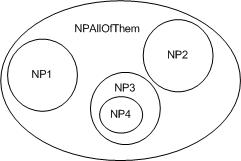
\includegraphics[width=5.5in]{images/Nodepool1.jpg}
      \caption{Nodepool Example}
      \label{fig:Nodepools1}
    \end{figure}

    In the figure below the Nodepools are incorrectly defined for two reasons:
    \begin{enumerate}
       \item NP1 and NP2 overlap.
       \item NP4 overlaps both nodepool ``NpAllOfThem'' and NP3.
    \end{enumerate}
    
    \begin{figure}[H]
      \centering
      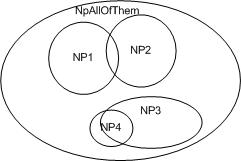
\includegraphics[width=5.5in]{images/Nodepool2.jpg}
      \caption{Nodepools: Overlapping Pools are Incorrect}
      \label{fig:Nodepools2}
    \end{figure}

    Multiple ``top-level'' nodepools are allowed.  A ``top-level'' nodepool has no containing
    pool.  Multiple top-level pools logically divide a cluster of machines into {\em multiple
      independent clusters} from the standpoint of the scheduler.  Work scheduled over one
    pool in no way affects work scheduled over the other pool.  The figure below shows an
    abstract nodepool configuration with two top-level nodepools, ``Top-NP1'' and ``Top-NP2''.
    \begin{figure}[H]
      \centering
      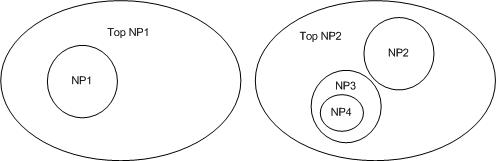
\includegraphics[width=5.5in]{images/Nodepool3.jpg}
      \caption{Nodepools: Multiple top-level Nodepools}
      \label{fig:Nodepools3}
    \end{figure}

\subsubsection{Scheduling considerations}
    A primary goal of the scheduler is to insure that no resources are left idle if there
    is pending work that is able to use those resources.  Therefore, work scheduled to
    a class defined over a specific nodepool (say, NpAllOfThem), may be scheduled on nodes
    in any of the nodepools contained within NpAllOfThem.  If work defined over a
    subpool (such as NP1) arrives, processes on nodes in NP1 that were scheduled for
    NpAllOfThem are considered {\em squatters} and are the most likely candidates for
    eviction. (Processes assigned to their proper nodepools are considered {\em residents}
    and are evicted only after all {\em squatters} have been evicted.)  The scheduler strives
    to avoid creating {\em squatters}.

    Because non-preemptable allocations can't be preempted, work submitted to a class
    implementing one of the non-preemptable policies (FIXED or RESERVE) are never allowed
    to ``squat'' in other nodepools and are only scheduled on nodes in their
    proper nodepool.

    In the case of multiple top-level nodepools: these nodepools and their sub-pools
    form independent scheduling groups.  Specifically,
    \begin{itemize}
        \item Fair-share allocations over any nodepool in one top-level pool do NOT affect the
          fair-share allocations for jobs in any other top-level nodepool.  Top-level nodepools
          define independently scheduled of resources within a single DUCC cluster.

        \item Work submitted to classes under one top-level nodepool do NOT get expanded to
          nodes under another top-level nodepool, even is there is sufficient capacity.
    \end{itemize}

    Most installations will want to assign the majority of nodes to a single top-level
    nodepool (or its subpools), using other top-level pools for nodes that cannot be
    shared with other work.

\subsubsection{Configuration}
\label{subsubsec:nodepool.configuration}
    DUCC uses simple named stanzas containing key/value pairs to configure nodepools.

    At least one nodepool definition is required.  This nodepool need not have any subpools or node
    definitions.  The first top-level nodepool is considered the ``default'' nodepool.  Any node not
    named specifically in one of the node files which checks in with DUCC is assigned to this
    first, {\em default} nodepool. 

    Thus, if only one nodepool is defined with no other attributes, all nodes are
    assigned to that pool.

    A nodepool definition consists of the token ``Nodepool'' followed by the 
    name of the nodepool, followed by a block delimited with ``curly'' braces \{ and \}.  This
    block contains the attributes of the nodepool as key/value pairs.
    Lineneds are ignored.  A semicolon ``$;$'' may optionally be used to
    delimit key/value pairs for readability, and an equals sign ``='' may optionally
    be used to delimit keys from values, also just for readability.  See the 
    \hyperref[fig:nodepool.configuration]{below}.

    The attributes of a Nodepool are:
    \begin{description}
      \item[domain] This is valid only in the ``default'' (first) nodepool.  Any node
        in any nodefile which does not have a domain, and any node which checks
        in to the Resource Manager without a domain name is assigned this domain name
        in order that the scheduler may deal entirely with full-qualified node names.

        If no {\em domain} is specified, DUCC will attempt to guess the domain based
        on the domain name returned on the node where the Resource Manager resides.

      \item[nodefile] This is the name of a file containing the names of the nodes
        which are members of this nodepool.

      \item[parent] This is used to indicate which nodepool is the logical parent.
        Any nodepool without a {\em parent} is considered a top-level nodepool.
    \end{description}
        
    The following example defines six nodepools, 
    \begin{enumerate}
      \item A top-level nodepool called ``--default--''.  All nodes not named
        in any nodefile are assigned to this nodepool.
      \item A top-level nodepool called ``jobdriver'', consisting of the nodes
        named in the file {\em jobdriver.nodes}.
      \item A subpool of ``--default--'' called ``intel'', consisting of the
        nodes named in {\em intel.nodes}.
      \item A subpool of ``--default--'' called ``power'', consisting of the
        nodes named in the file {\em power.nodes}.
      \item A subpool of ``intel'' called ``nightly-test'', consisting of the 
        nodes named in {\em nightly-test.nodes}.
      \item And a subpool of ``power'' called ``timing-p7'', consisting of the
        nodes named in {\em timing-p7.nodes}.
    \end{enumerate}

    \begin{figure}[H]
    
\begin{verbatim}
    Nodepool --default--  { domain mydomain.net }
    Nodepool jobdriver    { nodefile jobdriver.nodes }
    
    Nodepool intel        { nodefile intel.nodes        ; parent --default-- }
    Nodepool power        { nodefile power.nodes        ; parent --default-- }

    Nodepool nightly-test { nodefile nightly-test.nodes ; parent intel }
    Nodepool timing-p7    { nodefile timing-p7.nodes    ; parent power }
\end{verbatim}
      \caption{Sample Nodepool Configuration}
      \label{fig:nodepool.configuration}

    \end{figure}    


    \subsection{Class Definitions}
    \label{subsubsec:class.configuration}

    Scheduler classes are defined in the same simple block language as
    nodepools.

    A simple inheritance (or ``template'') scheme is supported for classes.  Any
    class may be configured to ``derive'' from any other class.  In this case, the
    child class acquires all the attributes of the parent class, any of which may
    be selectively overridden.  Multiple inheritance is not supported but
    nested inheritance is; that is, class A may inherit from class B which inherits
    from class C and so on. In this way, generalized templates for the site's
    class structure may be defined.  

    The general form of a class definition consists of the keyword Class, followed
    by the name of the class, and then optionally by the name of a ``parent'' class
    whose characteristics it inherits.   Following the name (and optionally parent class
    name) are the attributes of the class, also within a \{ block \} as for nodepools, and
    with lines and key/value pairs optionally delimited by  ``$;$'' and ``$=$'', respectively.
    See the sample \hyperref[fig:class.configuration]{below}.

    The attributes defined for classes are:
    \begin{description}

      \item[abstract] If specified, this indicates this class is a template ONLY. It is used
        as a model for other classes.  Values are ``true'' or ``false''.  The default is
        ``false''.  This class is never passed to the scheduler and may not be referenced
        by jobs.

      \item[debug] FAIR\_SHARE only. This specifies the name of a class to substitute
        for jobs submitted for debug.  For example, if class {\em normal} specifies
\begin{verbatim}
     debug = fixed
\end{verbatim}
        then any job submitted to this class with debugging requested is actually scheduled
        in class {\em fixed}. (For example, one probably does not want a debugging job
        scheduled as FAIR\_SHARE and possibly preempted, preferring the non-preemptable
        class {\em fixed}.

      \item[default] This specifies the class to be used as the default class for work submission
        if no class is explicitly given.  Only one class of type FAIR\_SHARE may contain this
        designation, in which case it names the default FAIR\_SHARE class.  Only one class of type
        FIXED\_SHARE or RESERVE may contain this designation, in which case it names the default
        class to use for reservations (Note that either FIXED\_SHARE or RESERVE scheduling policies
        are valid for reservations.)

      \item[expand-by-doubling] FAIR\_SHARE only.  If ``true'', and the {\em initialization-cap} is
        set, then after any process has initialized, the job will expand to its maximum allowable
        shares by doubling in size each scheduling cycle.  

        If not specified, the global value set in \hyperref[sec:ducc.properties]{ducc.properties} is used.

      \item[initialization-cap] FAIR\_SHARE only. If specified, this is the largest number of processes this job
        may be assigned until at least one process has successfully completed initialization.

        If not specified, the global value set in \hyperref[sec:ducc.properties]{ducc.properties} is used.

      \item[max-processes] FAIR\_SHARE and FIXED\_SHARE only.  This is the largest number of FIXED-SHARE,
        non-preemptable shares any single job may be assigned.

        Omit this property, or set it to 0 to disable the cap.

      \item[max-machines] RESERVE only.  This specifies the maximum number of full machines that
        may be reserved by any single job.

        Omit this property, or set it to 0 to disable the cap.

      \item[prediction-fudge] FAIR\_SHARE only. When the scheduler is considering expanding the
        number of processes for a job it tries to determine if the job may complete before those
        processes are allocated and initialized.  The {\em prediction-fudge} adds some amount of 
        time (in milliseconds) to the projected completion time.  This allows installations to
        prevent jobs from expanding when they were otherwise going to end in a few minutes
        anyway.

        If not specified, the global value set in \hyperref[sec:ducc.properties]{ducc.properties} is used.

      \item[nodepool] If specified, jobs for this class are assigned to nodes in this nodepool. The
        value must be the name of one of the configured nodepools.

      \item[policy] This is the scheduling policy, one of FAIR\_SHARE, FIXED\_SHARE, or RESERVE. This
        attribute is required (there is no default).

      \item[priority] This is the scheduling priority for jobs in this class.

      \item[weight] FAIR\_SHARE only. This is the fair-share weight for jobs in this class.
      
    \end{description}

    The following figure illustrates a representative class configuration for a large cluster,
    consisting of mixed Intel and Power nodes.  This class definition assumes the
    \hyperref[fig:nodepool.configuration]{nodepool configuration} shown above.  FAIR\_SHARE,
    FIXED\_SHARE, and RESERVE classes are defined over each machine architecture, Intel and Power,
    and over the combined pool. 

    \begin{figure}[H]    
\begin{verbatim}
# --------------------- Fair share definitions ---------------
Class fair-base {
      policy = FAIR_SHARE
      nodepool = intel
      priority = 10
      weight = 100
      abstract = true
      debug = fixed
}

Class nightly-test   fair-base  { weight = 100; nodepool nightly-test; priority = 7}

Class background     fair-base  { weight = 20 }
Class low            fair-base  { weight = 50 }
Class normal         fair-base  { weight = 100; default = true }
Class high           fair-base  { weight = 200 }
Class weekly         fair-base  { weight = 400 }

Class background-p7  background { nodepool = power }
Class low-p7         low        { nodepool = power }
Class normal-p7      normal     { nodepool = power }
Class high-p7        high       { nodepool = power }
Class weekly-p7      weekly     { nodepool = power }

Class background-all background { nodepool = --default-- }
Class low-all        low        { nodepool = --default-- }
Class normal-all     normal     { nodepool = --default-- }
Class high-all       high       { nodepool = --default-- }
Class weekly-all     weekly     { nodepool = --default-- }

# --------------------- Fixed share definitions ---------------
Class fixed-base {
      policy = FIXED_SHARE
      nodepool = intel
      priority = 5
      abstract = true
      max-processes = 10
}

Class fixed     fixed-base { }
Class fixed-p7  fixed-base { nodepool = power;    default = true; }
Class JobDriver fixed-base { nodepool = jobdriver; priority = 0 }      

# --------------------- Reserve definitions ---------------
Class reserve-base {
      policy = RESERVE
      nodepool = intel
      priority = 1
      abstract = true
      max-machines = 10
}
 
Class reserve     reserve-base { }
Class reserve-p7  reserve-base { nodepool = power }
Class timing-p7   reserve-base { nodepool = timing-p7 }
\end{verbatim}
          \caption{Sample Class Configuration}
      \label{fig:class.configuration}
    \end{figure}
    
\subsection{Validation}

The administrative command, \hyperref[subsec:admin.check-ducc]{\em check\_ducc} may be used to
validate a configuration, with the {\em -c} option.  This reads the entire configuration and
nodefiles, validates consistency of the definitions and insures the nodepools do not overlap.

During start-up, the \hyperref[subsec:admin.check-ducc]{\em start\_ducc} command always runs full validation, and if the
configuration is found to be incorrect, the cluster is not started.

Configuration checking is done internally by the DUCC java utility {\em
  org.apache.uima.ducc.commonNodeConfiguration}.  This utility contains a public
API as described in the Javadoc.  It may be invoked from the command line as follows:

    \paragraph{Usage:}
\begin{verbatim}
     java org.apache.uima.ducc.commonNodeConfiguration [-p] [-v nodefile] configfile
\end{verbatim}

    \paragraph{Options:}
    \begin{description}

      \item[$-p$] Pretty-print the compiled configuration to stdout. This illustrates
        nodepool nesting, and shows the fully-completed scheduling classes after inheritance.

      \item[$-v$ nodefile] This should be the master nodelist used to start DUCC.  This
        is assumed to be constructed to reflect the nodepool organization as 
        \hyperref[sec:admin-ducc.nodes]{described here}.  If provided,
        the nodepools are validated and checked for overlaps.

      \item[configfile] This is the name of the file containing the configuration.
    \end{description}
    

% 
% Licensed to the Apache Software Foundation (ASF) under one
% or more contributor license agreements.  See the NOTICE file
% distributed with this work for additional information
% regarding copyright ownership.  The ASF licenses this file
% to you under the Apache License, Version 2.0 (the
% "License"); you may not use this file except in compliance
% with the License.  You may obtain a copy of the License at
% 
%   http://www.apache.org/licenses/LICENSE-2.0
% 
% Unless required by applicable law or agreed to in writing,
% software distributed under the License is distributed on an
% "AS IS" BASIS, WITHOUT WARRANTIES OR CONDITIONS OF ANY
% KIND, either express or implied.  See the License for the
% specific language governing permissions and limitations
% under the License.
% 
\section{Ducc Node Definitions}
\label{sec:admin-ducc.nodes}
    The DUCC node definitions are specified by default in the file {\em ducc.nodes}.

    The DUCC node list is used to configure the nodes used to run jobs and assign reservations. 
    When DUCC is started, the nodelist is read an a DUCC Agent is started on every node in the list.

    The node list can be composed of multiple node lists to assist organization of the DUCC cluster. 
    All the administrative commands operate upon node lists. By carefully organized these lists it is 
    possible to administer portions of a cluster independently. 

    In particular, it is highly recommended that the nodelists reflect the nodepool structure.  In
    this way, the configuration used to start DUCC is guaranteed to match the nodeppool definitions.

    Several types of records are permitted in nodelists:
    \begin{description}

      \item[Comments] A comment is delimited with the symbol ``$\#$''.  All text on the line
        following this symbol is ignored.

      \item[import] If a line starts with the symbol {\em import}, the next symbol on that line
        is expected to be the name of another node list.  This permits the DUCC cluster's
        nodes to be configured in a structured manner.

        For instance, the file {\em ducc.nodes} might consist entirely of {\em import} statements
        naming all of the nodepool files.
      \item[domain] This must be the first line of the file.  If specified, it should name
        the default domain to be used for all the nodes in this file, and the nodes named
        in imported files.  If not specified, then during start-up, nodes without domain names are assigned
        domain names according to the global domain name specified in the \hyperref[subsubsec:nodepool.configuration]{Resource Manager configuration}
        file, and if none is specified there, the domain name on the host starting DUCC is used.

      \item[nodename] This is a single token consisting of the name of a node on which an
        agent it to be started.

    \end{description}

    The example below shows a partial, hypothetical node configuration corresponding to the
    \hyperref[fig:nodepool.configuration]{nodepool configuration} above.

    \begin{figure}[H]

\begin{verbatim}
> cat ducc.nodes
# import all the nodes corresponding to my nodepools 
domain my.domain
import intel.nodes
import power.nodes
import jobdriver.nodes
import nightly-test.nodes
import timing-p7.nodes

> cat intel.nodes
# import the intel nodes, by frame
import intel-frame1.nodes
import intel-frame2.nodes
import intel-frame3.nodes

>cat intel-frame1.nodes
#import the specific nodes from frame1
r1s1node1
r1s1node2
r1s1node3
r1s1node4
\end{verbatim}
      \caption{Sample Node Configuration}
      \label{fig:node.configuration}

    \end{figure}    
    


%% This is a section
% 
% Licensed to the Apache Software Foundation (ASF) under one
% or more contributor license agreements.  See the NOTICE file
% distributed with this work for additional information
% regarding copyright ownership.  The ASF licenses this file
% to you under the Apache License, Version 2.0 (the
% "License"); you may not use this file except in compliance
% with the License.  You may obtain a copy of the License at
% 
%   http://www.apache.org/licenses/LICENSE-2.0
% 
% Unless required by applicable law or agreed to in writing,
% software distributed under the License is distributed on an
% "AS IS" BASIS, WITHOUT WARRANTIES OR CONDITIONS OF ANY
% KIND, either express or implied.  See the License for the
% specific language governing permissions and limitations
% under the License.
% 

\section{Administrative Commands}

   The administrative commands include a command to start DUCC, one to stop it, and one to 
   verify the configuration and query the state of the cluster.

   Note: The scripting that supports these functions runs (by default) in multi-threaded mode so
   large clusters can be started, stopped, and queried quickly.  If DUCC is running on an older
   system, the threading may not work right, in which case the scripts detect this and run
   single-threaded.  As well, all these commands support a ``--nothreading'' option to manually
   disable the threading.

\subsection{start\_ducc}
\label{subsec:admin.start-ducc}

    \subsubsection{{\em Description}}
    The command \ducchome/admin/start\_ducc is used to start DUCC processes. If run with no parameters
    it takes the following actions:
    \begin{itemize}
      \item Starts the management processes Resource Manager, Orchestrator, Process Manager,      
      Services Manager, and Web Server on the local node (where start\_ducc is executed.       
      \item Starts an agent process on every node named in the default node list. 
    \end{itemize}

    \subsubsection{{\em Usage}}

    \begin{description}
      \item[start\_ducc {[options]}] \hfill \\ 
        If no options are given, all DUCC processes are started, using the default node list, 
        {\em ducc.nodes}. 
      
      \end{description}
      
      \subsubsection{{\em Options: }}
      \begin{description}

        \item[-n, --nodelist {[nodefile] }] \hfill \\
          Start agents on the nodes in the nodefile. Multiple nodefiles may be specified: 
\begin{verbatim}
start\_ducc -n foo.nodes -n bar.nodes -n baz.nodes 
\end{verbatim}
          

        \item[-c, --component {[component] }] \hfill \\
          Start a specific DUCC component, optionally on a specific node. If the component 
          name is qualified with a nodename, the component is started on that node. To qualify 
          a component name with a destination node, use the notation component@nodename. 
          Multiple components may be specified: 
\begin{verbatim}
start\_ducc -c sm -c pm -c rm -c or@bj22 -c agent@n1 -c agent@n2 
\end{verbatim}
          
          Components include: 
          \begin{description}
            \item[rm] The Resource Manager
            \item[or]The Orchestrator
            \item[pm]The Process Manager
            \item[sm]The Service Manager
            \item[ws]The Web Server
            \item[agent]Node Agents
          \end{description}

          \item[--nothreading] If specified, the command does not run in multi-threaded mode
            even if it is supported on the local platform.

      \end{description}

      \subsubsection{{\em Notes: }}
      A different nodelist may be used to specify where Agents are started. As well multiple node 
      lists may be specified, in which case Agents are started on all the nodes in the multiple node 
      lists. 
      
      To start only agents, run start\_ducc specifying a nodelist explicitly. When started like this, the 
      management daemons are not started unless explicitly requested. 
      
      To start only management processes, run start\_ducc with the -m or --management flags. When 
      started like the the agents are not started unless explicitly requested. 
      
      To start a specific management process, run start\_ducc with the -c component parameter, 
      specify the component that should be started. 
      
      \subsubsection{{\em Examples: }}

      Start some nodes from two different nodelist.  This doesn't start any of the management processes
      but it does insure the ActiveMQ Broker is available.
\begin{verbatim}
        start\_ducc -n foo.nodes -n bar.nodes 
\end{verbatim}
                  
      Start an agent on a specific node: 
\begin{verbatim}
        start\_ducc -c agent@a.specific.node 
\end{verbatim}
      
      Start the webserver on node 'bingle': 
\begin{verbatim}
        start\_ducc -c ws@bingle 
\end{verbatim}

      \subsubsection{{\em Debugging:}}

      Sometimes something will not start and it can be difficult to understand why.  To diagnose, it is
      helpful to know that {\em start\_ducc} is simply a wrapper around a lower-level bit of scripting
      that does the actual work.  That lower-level code can be invoked stand-alone, in which case
      console messages that {\em check\_ducc} will have suppressed are presented to the console.

      The lower-level script is called {\em ducc.py} and accepts the same {\em -c component} flag as
      start\_ducc.  If some component will not start, try running {\em ducc.py -c component} directly.
      It will start in the foreground and usually the cause of the problem becomes evident from
      the console.

      For example, suppose the Resource Manager will not start.  Run the following:
\begin{verbatim}
      ./ducc.py -c rm
\end{verbatim}
      and examine the output.  Use {\em CTL-C} to stop the component when done.
      

\subsection{stop\_ducc}
\label{subsec:admin.stop-ducc}

    \subsubsection{{\em Description:}}
    Stop\_ducc is used to stop DUCC processes. If run with no parameters it takes the following 
    actions:
    \todo Garbled by maven or docbook, update this

    \subsubsection{\em Usage:}

    \begin{description}
      \item[stop\_ducc {[options]}] \hfill \\ 
        If no options are given, help text is presented. At least one option is required, to avoid 
        accidental cluster shutdown. 
      \end{description}
    

      \subsubsection{Options:}
        \begin{description}

          \item[-a --all] \hfill \\
            Stop all the DUCC processes, including agents and management processes. This 
            broadcasts a "shutdown" command to all DUCC processes. Shutdown is normally 
            performed gracefully will all process including job processes given time to save state. 
            All user processes, both jobs and services, are sent shutdown signals. Job and service 
            processes which do not shutdown within a designated grace period are then forcibly 
            terminated with kill -9. 
            
          \item[-n, --nodelist [nodefile]] \hfill \\
            Only the DUCC agents in the designated nodelists are shutdown. The processes are sent 
            kill -INT signals which triggers the Java shutdown hooks and enables graceful shutdown. 
            All user processes on the indicated nodes, both jobs and services, are sent "shutdown" 
            signals and are given a minute to shutdown gracefully. Job and service processes which do 
            not shutdown within a designated grace period are then forcibly terminated with kill -9. 
            
\begin{verbatim}
stop\_ducc -n foo.nodes -n bar.nodes -n baz.nodes 
\end{verbatim}

          \item[-c, --component [component]] \hfill \\
            Stop a specific DUCC component. 

            This may be used to stop an errant management component and subsequently restart it 
            (with start\_ducc). 
            
            This may also be used to stop a specific agent and the job and services processes it is
            managing, without the need to specify a nodelist.  
            
            Examples: 

            Stop agents on nodes n1 and n2:
\begin{verbatim}
stop_ducc -c agent@n1 -c agent@n2 
\end{verbatim}
            
            Stop and restart the rm: 
\begin{verbatim}
stop_ducc -c rm 
start_ducc -c rm
\end{verbatim}
            
            Components include: 
            \begin{description}
              \item[rm] The Resource Manager.                 
              \item[or] The Orchestrator.                 
              \item[pm] The Process Manager.                 
              \item[sm] The Service Manager.                 
              \item[ws] The Web Server.                 
              \item[broker] The ActiveMQ broker (only if the broker is auto-managed).
              \item[agent\@node] Node Agent on the specified node.
              \end{description}

          \item[--nothreading] If specified, the command does not run in multi-threaded mode
            even if it is supported on the local platform.
              
       \end{description}
            
   \subsubsection{{\em Notes:}}
   Sometimes problems in the network or elsewhere prevent the DUCC components from stopping properly.  The
   {\em check\_ducc} command, described in the following section, contains options to query the
   existance of DUCC processes in the cluster, to forcibly ({\em kill -9}) terminate them, and to
   more gracefully terminate them ({\em kill -INT}).
          


\subsection{check\_ducc}
\label{subsec:admin.check-ducc}
    \subsubsection{{\em Description:}}

    Check\_ducc is used to verify the integrity of the DUCC installation and to find and report on
    DUCC processes. It identifies processes owned by ducc (management processes, agents,
    and job processes), and processes started by DUCC on behalf of users.
    
    Check\_ducc can also be used to clean up errant DUCC processes when stop\_ducc is unable 
    to do so. The difference is that stop\_ducc generally tries more gracefully stop processes. 
    check\_ducc is used as a last resort, or if a fast but graceless shutdown is desired. 
    
    \subsubsection{\em{Usage: }}

        \begin{description} 
          \item[check\_ducc {[options]}]
              If no options are given this is the equivalent of: 
\begin{verbatim}
check_ducc -c -n ../resources/ducc.nodes 
\end{verbatim}
              
              This verifies the integrity of the DUCC installation and searches for all the
              processes owned by user {\em ducc} and started by DUCC on all the nodes in ducc.nodes.
        \end{description}
            
     \subsubsection{\em{Options:}}
         \begin{description}
           \item[-n --nodelist {[nodefile]}]
             Only the nodes specified in the nodefile are searched. The option may be specified 
             multiple times for multiple nodefiles. Note that the "local" node is always checked as well. 
\begin{verbatim}
check_ducc -n nlist1 -n nlist2 
\end{verbatim}
                       
           \item[-c --configuration]
             Verify the \hyperref[sec:ducc.classes]{Resource Manager configuration}.

           \item[-p --pids]               
               Rewrite the PID file. The PID file contains the process ids of all known DUCC 
               management and agent processes. The PID file is normally managed by start\_ducc and 
               stop\_ducc and is stored in the file {\em ducc.pids} in directory {\em ducc\_runtime/state}.
               
               Occasionally the PID file can become partially or fully corrupted; for example, if a DUCC 
               process dies spontaneously. Use check\_ducc -p to search the cluster for processes and 
               refresh the PID file. 
               
            \item[-i, --int] \hfill \\
              Use this to send a shutdown signal ({\em kill -INT}) to all the DUCC processes.  The DUCC processes
              catch this signal, close their resources and exit.  Some resources take some time to close, or in
              case of problems, are unable to close, in which case the DUCC processes will unconditionally exit.

              Sometimes problems in the network or elsewhere prevent {\em check\_ducc -i} from terminating
              the DUCC processes.  In this case, use {\em check\_ducc -k}, described below.

            \item[-k, --kill] \hfill \\
              Use this to forcibly kill a component using kill -9. This should only be used if {\em stop\_ducc}
              or {\em check\_ducc -i} does not work.  

            \item[-s, --single\_user] \hfill \\
              Bypass the multi-user permission checks normally done on the ducc\_ling utility.
              
            \item[--nothreading] If specified, the command does not run in multi-threaded mode
              even if it is supported on the local platform.

            \item[-v, --verboase] \hfill \\
              When specified with {\em -c} to check the configuration, this emits a formatted version
              of the node list showing the full structure of the scheduling classes.
              

           \end{description}               

\subsection{rm\_reconfigure}
\label{subsec:admin.rm-reconfigure}

    \subsubsection{{\em Description:}}
    Rm\_reconfigure is used to force the Resource Manager (RM) to reread all its configuration
    files and reconfigure itself accordingly, without the need to fully stop and restart RM.
    This is generally much faster than RM restart and avoids losing most state messages from
    the other DUCC processes.
    
    The {\em rm\_reconfigure} command first performs a 
    \hyperref[sec:admin.properties-merge]{properties merge.}

    RM then validates the new
    configuration, and if no errors are found, saves certain information such as current node
    online-offline status.  It then rereads the following configuration files and rebuilds its
    internal structures accordingly:
    \begin{itemize}
      \item ducc.properties (after merging default.ducc.properties and site.ducc.properties,
      \item ducc.classes,
      \item log4j.xml.
    \end{itemize}
    The saved configuration is then restored into the newly configured structures.
    On receipt of the next Orchestrator state, the RM fully rebuilds its state from the current
    DUCC load and scheduling restarts.

    Depending on the nature of the new configuration, the current load may be adjusted; for
    example, if the weight of a fair-share class is changed, preemptions or extra allocations
    may be performed.

    If the new configuration is not consistent with the current load, a number of more drastic
    adjustments will be performed:
    \begin{itemize}
      \item If a fair-share class is deleted, all existing jobs for that class are preempted
        and a {\em refusal} message is sent to the Orchestrator for each affected job.
      \item If a fair-share class is redefined over a different nodepool such that existing
        work are no longer legally scheduled, any shares allocated over inappropriate
        hosts are {\em preempted}.  As soon as the preemptions are acknowledged, the RM
        will reschedule the shares over the differently-configured resources.
      \item If a non-preemptable class is deleted or reconfigured so existing non-preempt able
        work is no longer allocated correctly, the following will occur:
        \begin{itemize}
            \item If the shares are for services, they are deallocated and a {\em refusal} is
              sent to the Orchestrator.  The Service Manager will observe this and restart the
              processes, causing them to be reallocated over the changed configuration.
            \item Otherwise, the RM leaves the allocation in place, but places the hosts on an
              internal {\em blacklist}, preventing subsequent scheduling to those hosts. Once
              the (now) incorrectly placed shares are freed (e.g. by canceling a reservation or
              exit of a managed reservation), the hosts are again white listed and made available
              for scheduling.
        \end{itemize}
     \end{itemize}
        
    In short, the RM makes every effort to avoid disturbing existing allocations, and blacklists
    hosts that are no longer consistently configured for the current load, until such time as
    the allocations on those hosts are released.

    \subsubsection{\em Usage:}

    \begin{description}
      \item[rm\_reconfigure] \hfill \\ 
        This command has no options.
      \end{description}
             
       


\subsection{rm\_qload}
\label{subsec:admin.rm-qload}

    \subsubsection{{\em Description:}}
    Rm\_qload is used to query the Resource Manager's scheduling tables to determine the
    current demand and capacity of the system, as the RM sees it.  The primary purpose
    is to provide information to adjunct resource managers (such as a ``cloud'') to
    determine the current needs, or lack thereof, of the system.  The administrative
    command is implemented as a Python script that interacts with the underlying
    Java ``RmQueryLoadReply'' API and is provided mostly as an example of how
    scripting can be used to interact with the RM.

    After displaying the current scheduling quantum, the response is provided in two sections:
    \begin{enumerate}
      \item Information showing the current demand and usage of resource classes, and
      \item Information showing the current nodepool usage.
    \end{enumerate}

    \subsubsection{\em Class section}
    Three lines are emitted per class:
    \begin{enumerate}
      \item The name of the class and its scheduling policy,
      \item A line showing the {\em demand}, or {\em request} by quantum, on the class, and
      \item A line showing the {\em usage}, or {\em award}, by quantum on the class.
    \end{enumerate}
    
    The numbers shown for {\em request} and {\em award} show the number of processes, by
    memory, in terms of scheduling quantum, for each class.  For example, assuming the
    scheduling quantum is 15GB, the following shows:
    \begin{itemize}
      \item Five processes of quantum 2 (15-30GB) are requested, but only two have been awarded,
      \item Three processes of quantum 3 (31-45GB) are requested and all have been awarded,
      \item Four processes of quantum 4 (46-60GB) are requested, and two have been awarded.
    \end{itemize}
\begin{verbatim}
Class normal policy FAIR_SHARE
   requested    0    0    5    3    4    0    0    0    0 
   awarded      0    0    2    3    2    0    0    0    0 
\end{verbatim}

    \subsubsection{\em Nodepool section}
    Six lines are displayed for each nodepool:
    \begin{enumerate}
      \item The name of the nodepool,
      \item A summary showing the number hosts in the pool which are online, dead (unresponsive), and
          varied-off, the total quantum shares available to the nodepool, and the total unscheduled or 
          {\em free} shares.
      \item The number of hosts known to the nodepool, by quantum, similar to the class listings above,
      \item The nubmer of online hosts, by quantum,
      \item The number of completely free hosts by quantum (no work currently scheduled), and
      \item The number of {\em virtual} hosts, by quantum.  A {\em virtual host} is created when a
          host is partially scheduled.  For example, if a 32G processes is scheduled on a 64G host, this
          creates one free 32G {\em virtual host}.
    \end{enumerate}
    To determine the number of processes, by quantum, that can be scheduled, one must {\em sum} the
    ``free'' and ``virtual'' columns.
    
    For example, (assuming a 15GB quantum), the following listing shows
    that nodepool ``power'' contains fourteen hosts with at least 45GB each (3 quanta).  Two
    of these hosts have something scheduled on them (the ``free
    machines'' line), leaving unused space of one 15G quantum on one
    host, and one 30GB quantum on another host.

\begin{verbatim}
Nodepool power
   online 14 dead 0 offline 0 total-shares 42 free-shares 42
   all     machines:    0    0    0   14    0    0    0    0    0 
   online  machines:    0    0    0    0    0    0    0    0    0 
   free    machines:    0    0    0   12    0    0    0    0    0 
   virtual machines:    0    1    1    0    0    0    0    0    0 
\end{verbatim}

    \subsubsection{\em Usage:}
    \begin{description}
      \item[rm\_qload] \hfill \\ 
        This command has no options.
      \end{description}
             
       
\subsection{rm\_qoccupancy}
\label{subsec:admin.rm-qoccupancey}

    \subsubsection{{\em Description:}}
    Rm\_qoccupancy provides a list of all known hosts to the RM, and for each host, the following information:
    \begin{itemize}
      \item The name of the host,
      \item Whether the host has any blacklists processes on it,
      \item Whether the host is currently onlline (responsive),
      \item The status of the host; whether the host is schedulable ({\em up} or {\em down}.  A responsive host becomes
        unschedulable ({\em down}) if it is varied-off,
      \item The nodepool the host is a member of,
      \item The reported memory size of the host, 
      \item The {\em order} of the host.  The {\em order} is defined to be the maximum number of quantum shares
        supported by the host,
      \item The number of unscheduled quantum shares on the host, and
      \item If work is scheduled on the host, information relevent to that scheduled processes (or reservation).
    \end{itemize}

    If work is scheduled on a host, the work summary is keyed thus:
    \begin{description}
      \item[J] The Orchestrator-assigned job id of the work,
      \item[S] The RM-assigned share id of the work,
      \item[O] The {\em order} of the allocation; that is, the number of quantum shares the allocation occupies,
      \item[II] The {\em initialization investment}; the number of milliseconds the allocated work spent in its
        initialization phase, if any (usually only UIMA-AS processes display this),
      \item[IR] The {\em runtime investment}; the number of milliseconds spent processing the current CASs, if this
        is a UIMA-AS processes.  Note that this number can change dramatically, as it is the sum of time spent only
        by the current CASs.  When a CAS completes, it no longer contributes to the investment of the process.  The RM
        uses this information to determine the best candidate for eviction, if needed ot maintain fair-share.
      \item[E] Whether the RM has preempted (evicted) the process but it has not yet exited,
      \item[P] Whether the RM has purged the process (evicted, because the host is non-responsive), but it has not
        been confirmed evicted,
      \item[F] Whether the process is {\em fixed}; that is, non-preemptbable,
      \item[I] Whether the initialization phase is completed (usually only UIMA-AS processes).
    \end{description}

    The following example shows seven hosts, one with a preemptable share in the {\em --default--}
    nodepool (on bluej290-5), and one with a non-preemptable share in the {\em jobdriver} nodepool.
\begin{verbatim}
                Node Blacklisted Online Status        Nodepool     Memory Order   Free
          bluej290-5       False   True     up     --default--   32505856     2      0
                    J[    6006] S[     189] O[2] II[       0] IR[       0] E[False] P[False] F[False] I[False]

          bluej290-6       False   True     up     --default--   32505856     2      2
          bluej290-7       False   True     up     --default--   32505856     2      2
         bluej291-26       False   True     up    nightly-test   32505856     2      2
         bluej291-27       False   True     up    nightly-test   32505856     2      2
         bluej293-60       False   True     up           intel   32505856     2      2
         bluej537-73       False   True     up       jobdriver   32505856     2      1
                    J[    5973] S[       1] O[1] II[       0] IR[       0] E[False] P[False] F[ True] I[False]


\end{verbatim}


    \subsubsection{\em Usage:}

    \begin{description}
      \item[rm\_qoccupancy] \hfill \\ 
        This command has no options.
      \end{description}
             
       

\subsection{vary\_off}
\label{subsec:admin.vary-off}
    \subsubsection{{\em Description:}}

    Vary\_off is used to remove a host from scheduling and to evict the work that is running on it.
    This allows for graceful clearance of a host so the host can be take offline for maintenance,
    or any other purpose (such as sharing the host with other applications.)  The DUCC agent
    is NOT stoppped; use 
    \hyperref[subsec:admin.stop-ducc]{stop\_ducc} to stop the agent.  Reservations are not 
    canceled by {\em vary\_off}.
    
    Only the userid that started DUCC may issue {\em vary\_off}; attempts from other userids
    are rejected.

    \subsubsection{\em{Usage: }}

        \begin{description} 
          \item[vary\_off list-of-hosts]
            The {\em list-of-nodes} is a space delimited list of host to be removed from
              scheduling in the DUCC cluster.
        \end{description}
            
\subsection{vary\_on}
\label{subsec:admin.vary-on}
    \subsubsection{{\em Description:}}

    Vary\_on is used to restore a host to scheduling by DUCC.  If the agent is still
    alive the host becomes immediately available.  The agent is not started by
    {\em vary\_on}; use use 
    \hyperref[subsec:admin.start-ducc]{start\_ducc} to start the agent if needed.

    Only the userid that started DUCC may issue {\em vary\_on}; attempts from other userids
    are rejected.
    
    \subsubsection{\em{Usage: }}

        \begin{description} 
          \item[vary\_on list-of-hosts]
            The {\em list-of-nodes} is a space delimited list of host to be restored for
              scheduling in the DUCC cluster.
        \end{description}
            
       


%%\input{part4/admin/stop-ducc.tex}
%%\input{part4/admin/check-ducc.tex}
%%\input{part4/admin/ducc-post-install.tex}
%%\input{part4/admin/ducc-statedump.tex}
%%\input{part4/admin/verify-ducc.tex}


%% This should input a chapter
% 
% Licensed to the Apache Software Foundation (ASF) under one
% or more contributor license agreements.  See the NOTICE file
% distributed with this work for additional information
% regarding copyright ownership.  The ASF licenses this file
% to you under the Apache License, Version 2.0 (the
% "License"); you may not use this file except in compliance
% with the License.  You may obtain a copy of the License at
% 
%   http://www.apache.org/licenses/LICENSE-2.0
% 
% Unless required by applicable law or agreed to in writing,
% software distributed under the License is distributed on an
% "AS IS" BASIS, WITHOUT WARRANTIES OR CONDITIONS OF ANY
% KIND, either express or implied.  See the License for the
% specific language governing permissions and limitations
% under the License.
% 
% Create well-known link to this spot for HTML version
\ifpdf
\else
\HCode{<a name='DUCC_RM'></a>}
\fi
\chapter{Resource Management}
\label{chap:rm}
    \section{Overview}

    The DUCC Resource Manager is responsible for allocating cluster resources among the various 
    requests for work in the system. DUCC recognizes several classes of work: 

    \begin{description}
        \item[Managed Jobs]
            Managed jobs are Java applications implemented in the UIMA framework. 
            and are scaled out by DUCC using UIMA-AS. Managed jobs are executed as some 
            number of discrete processes distributed over the cluster resources. All processes of all jobs 
            are by definition preemptable; the number of processes is allowed to increase and decrease 
            over time in order to provide all users access to the computing resources. 
        \item[Services]
            Services are long-running processes which perform some function on behalf of 
            jobs or other services. Most DUCC services are UIMA-AS assigned to a non-preemptable 
            resource class, as defined below.

        \item{Reservations}
            A reservation provides non-preemptable, persistent, dedicated use of a full machine or
            some part of a machine to a specific user.

        \item{Arbitrary Processes}
            An {\em arbitrary process} or {\em managed reservation} is any process at all, which may
            or may not have anything to do with UIMA.  These processes are usually used for services,
            or to launch very large Eclipse work-spaces for debugging.  DUCC supports this type of 
            process but is not optimized for it.  These processes are usually scheduled to be 
            non-preemptable, occupying either a dedicated machine or some portion of a machine.

      \end{description}
          
    In order to apportion the cumulative memory resource among requests, the Resource Manager 
    defines some minimum unit of memory and allocates machines such that a "fair" number of 
    "memory units" are awarded to every user of the system. This minimum quantity is called a share 
    quantum, or simply, a share. The scheduling goal is to award an equitable number of memory 
    shares to every user of the system. 

    The Resource Manager awards shares according to a fair share policy. The memory shares in a 
    system are divided equally among all the users who have work in the system. Once an allocation 
    is assigned to a user, that user's jobs are then also assigned an equal number of shares, out of the 
    user's allocation. Finally, the Resource Manager maps the share allotments to physical resources. 
    
    To map a share allotment to physical resources, the Resource Manager considers the amount of 
    memory that each job declares it requires for each process. That per-process memory requirement 
    is translated into the minimum number of collocated quantum shares required for the process to 
    run. 
    
    For example, suppose the share quantum is 15GB. A job that declares it requires 14GB per process 
    is assigned one quantum share per process. If that job is assigned 20 shares, it will be allocated 20 
    processes across the cluster. A job that declares 28GB per process would be assigned two quanta 
    per process. If that job is assigned 20 shares, it is allocated 10 processes across the cluster. Both     
    jobs occupy the same amount of memory; they consume the same level of system resources. The 
    second job does so in half as many processes however. 
    
    The output of each scheduling cycle is always in terms of processes, where each process is allowed 
    to occupy some number of shares. The DUCC agents implement a mechanism to ensure that no 
    user's job processes exceed their allocated memory assignments. 
    
    Some work may be deemed to be more "important" than other work. To accommodate this, DUCC 
    allows jobs to be submitted with an indication of their relative importance: more important jobs are 
    assigned a higher "weight"; less important jobs are assigned a lower weight. During the fair share 
    calculations, jobs with higher weights are assigned more shares proportional to their weights; jobs 
    with lower weights are assigned proportionally fewer shares. Jobs with equal weights are assigned 
    an equal number of shares. This weighed adjustment of fair-share assignments is called weighted 
    fair share. 
    
    The abstraction used to organized jobs by importance is the job class or simply ``class''. As jobs enter 
    the system they are grouped with other jobs of the same importance and assigned to a common 
    class. The class abstraction and its attributes are described in \hyperref[sec:rm.job-classes]{subsequent sections}. 
    
    The scheduler executes in two phases: 
    \begin{enumerate}
        \item The How-Much phase: every job is assigned some number of shares, which is converted to the
          number of processes of the declared size.
        \item The What-Of phase: physical machines are found which can accommodate the number of
          processes allocated by the How-Much phase. Jobs are mapped to physical machines such that
          the total declared per-process amount of memory does not exceed the physical memory on the
          machine.  
    \end{enumerate}
      
    The How-Much phase is itself subdivided into three phases:
    \begin{enumerate}
        \item Class counts:Apply weighed fair-share to all the job classes that have jobs assigned to
          them. This apportions all shares in the system among all the classes according to their
          weights.  

        \item User counts: For each class, collect all the users with jobs submitted to that
          class, and apply fair-share (with equal weights) to equally divide all the class shares among
          the users. This apportions all shares assigned to the class among the users in this class.  A
          user may have jobs in more than one class, in which case that user's fair share is calculated
          independently within each class.
          
        \item Job counts: For each user, collect all jobs
          assigned to that user and equally divide all the user's shares among
          the jobs. This apportions all shares given to this user for each class among the user's
          jobs in that class. 
    \end{enumerate}

    Reservations are relatively simple. If the number of shares or machines requested is available
    the reservation succeeds immediately.  If a sufficient number of co-located shares can be made
    available through preemption of fair-share jobs, preemptions are scheduled and the reservation
    is deferred until space becomes available.  resources are allocated. If space cannot be found by
    means of preemption, the reservation fails.


    \section{Scheduling Policies}

    The Resource Manager implements three coexistent scheduling policies. 
    \begin{description}
        \item[FAIR\_SHARE] This is the weighted-fair-share policy described in detail above.

        \item[FIXED\_SHARE] The FIXED\_SHARE policy is used to reserve a portion of a machine. The
          allocation is non-preemptable and remains active until it is canceled.

          FIXED\_SHARE allocations have several uses:
          \begin{itemize}
            \item As reservations.  In this case DUCC starts no work in the share(s); the user must
              log in (or run something via ssh), and then manually release the reservation to free
              the resources.  This is often used for testing and debugging.
            \item For services.  If a service is registered to run in a FIXED\_SHARE allocation,
              DUCC allocates the resources, starts and manages the service, and releases the
              resource if the service is stopped or unregistered.
            \item For UIMA jobs.  A ``normal'' UIMA job may be submitted to a FIXED\_SHARE
              class.  In this case, the processes are never preempted, allowing constant and
              predictable execution of the job.  The resources are automatically released when
              the job exits.
          \end{itemize}
          
          {\em Note:} A fixed-share request specifies a number of processes of a given size, for example, "10 
          processes of 32GB each". The ten processes may or may not be collocated on the same 
          machine. Note that the resource manager attempts to minimize fragmentation so if there is a 
          very large machine with few allocations, it is likely that there will be some collocation of the 
          assigned processes. 
          
          {\em Note:} A fixed-share allocation may be thought of a reservation for a "partial" machine. 
          
        \item[RESERVE] The RESERVE policy is used to reserve a full machine. It always returns an
          allocation for an entire machine. The reservation is permanent (until it is canceled) and
          it cannot be preempted by any other request.

          Reservations may also be used for services or UIMA jobs in the same way as FIXED\_SHARE 
          allocations, the difference being that a reservation occupies full machines and FIXED\_SHARE
          occupies portions of a machine.

          {\em Note:} It is possible to configure the scheduling policy so that a reservation returns any machine in 
          the cluster that is available, or to restrict it to machines of the size specified in the reservation 
          request. 
    \end{description}
    
    \section{Priority vs Weight}

    It is possible that the various policies may interfere with each other. It is also possible that
    the fair share weights are not sufficient to guarantee sufficient resources are allocated to
    high importance jobs. Priorities are used to resolve these conflicts

    Simply: priority is used to specify the order of evaluation of the job classes. Weight is used
    to proportionally allocate the number of shares to each class under the weighted fair-share
    policies.

    \paragraph{Priority.} It is possible that conflicts may arise in scheduling policies. For example, it may be
    desired that reservations be fulfilled before any fair-share jobs are scheduled. It may be
    desired that some types of jobs are so important that when they enter the system all other
    fair-share jobs be evicted. Other such examples can be found.
    
    To resolve this, the Resource Manager allows job classes to be prioritized. Priority is
    used to determine the order of evaluation of the scheduling classes.
    
    When a scheduling cycle starts, the scheduling classes are ordered from "best" to "worst" priority. 
    The scheduler then attempts to allocate ALL of the system's resources to the "best" priority class. 
    If any resources are left, the scheduler proceeds to schedule classes in the next best
    priority, and so on, until either all the 
    resources are exhausted or there is no more work to schedule. 
    
    It is possible to have multiple job classes of the same priority. What this means is that resources 
    are allocated for the set of job classes from the same set of resources. Resources for higher priority 
    classes will have already been allocated, resources for lower priority classes may never become 
    available. 
    
    To constrain high priority jobs from completely monopolizing the system, class caps may be 
    assigned. Higher priority guarantees that some resources will be available (or made available) but 
    doesn't require that all resources necessarily be used. 

    \paragraph{Weight.} Weight is used to determine the relative importance of jobs in a set of job classes of 
    the same priority when doing fair-share allocation. All job classes of the same priority are assigned 
    shares from the full set of available resources according to their weights using weighted fair-share. 
    Weights are used only for fair-share allocation. 
    
    \section{Node Pools}
    It may be desired or necessary to constrain certain types of resource allocations to a specific
    subset of the resources. Some nodes may have special hardware, or perhaps it is desired to
    prevent certain types of jobs from being scheduled on some specific set of machines. Nodepools
    are designed to provide this function.

    Nodepools impose hierarchical partitioning on the set of available machines. A nodepool is a
    subset of the full set of machines in the cluster. Nodepools may not overlap. A nodepool may
    itself contain non-overlapping subpools.  It is possible to define and schedule work to
    multiple, independent nodepools.

    Job classes are associated with nodepools. During scheduling, a job may be assigned resources
    from its associated nodepool, or from any of the subpools which divide the associated nodepool.
    The scheduler attempts to fully exhaust resources in the associated nodepool before allocating
    within the subpools, and during eviction, attempts to first evict from the subpools. The
    scheduler ensures that the nodepool mechanism does not disrupt fair-share allocation.
    
    More information on nodepools and their configuration can be \hyperref[subsec:nodepools]{found here}.

    \section{Job Classes}
    \label{sec:rm.job-classes}
    The primary abstraction to control and configure the scheduler is the class. A class is simply a set 
    of rules used to parametrize how resources are assigned to jobs. Every job that enters the system is 
    associated with a single job class. 
    
    The job class defines the following rules: 
    
    \begin{description}
        \item[Priority] This is the order of evaluation and assignment of resources to this class. See
          the discussion of priority vs Weight for details. 

        \item[Weight] This defines the "importance" of jobs in this class and is used in the weighted
          fair-share calculations. 

        \item[Scheduling Policy] This defines the policy, fair share, fixed share, or reserve used to
          schedule the jobs in this class.

        \item[Cap] Class caps limit the total resources assigned to a class. This is designed to prevent
          high importance and high priority job classes from fully monopolizing the resources. It can be
          used to limit the total resources available to lower importance and lower priority classes.

        \item[Nodepool] A class may be associated with exactly one nodepool. Jobs submitted to the class
          are assigned only resources which lie in that nodepool, or in any of the subpools defined
          within that nodepool.

        \item[Prediction] For the type of work that DUCC is designed to run, new processes typically take
          a great deal of time initializing. It is not unusual to experience 30 minutes or more of
          initialization before work items start to be processed.

          When a job is expanding (i.e. the number of assigned processes is allowed to dynamically 
          increase), it may be that the job will complete before the new processes can be assigned and 
          the work items within them complete initialization. In this situation it is wasteful to allow the 
          job to expand, even if its fair-share is greater than the number of processes it currently has 
          assigned. 
          
          By enabling prediction, the scheduler will consider the average initialization time for processes 
          in this job, current rate of work completion, and predict the number of processes needed to 
          complete the job in the optimal amount of time. If this number is less than the job's fair, share, 
          the fair share is capped by the predicted needs. 
          
        \item[Prediction Fudge] When doing prediction, it may be desired to look some time into the
          future past initialization times to predict if the job will end soon after it is expanded. The
          prediction fudge specifies a time past the expected initialization time that is used to
          predict the number of future shares needed.

        \item[Initialization cap] Because of the long initialization time of processes in most DUCC jobs,
          process failure during the initialization phase can be very expensive in terms of wasted
          resources. If a process is going to fail because of bugs, missing services, or any other
          reason, it is best to catch it early.

          The initialization cap is used to limit the number of processes assigned to a job until it is 
          known that at least one process has successfully passed from initialization to running. As soon 
          as this occurs the scheduler will proceed to assign the job its full fair-share of resources. 

        \item[Expand By Doubling] Even after initialization has succeeded, it may be desired to throttle
          the rate of expansion of a job into new processes.

          When expand-by-doubling is enabled, the scheduler allocates either twice the number of 
          resources a job currently has, or its fair-share of resources, whichever is smallest. 

        \item[Maximum Shares] This is for FIXED\_SHARE policies only. Because fixed share allocations are
          not preemptable, it may be desirable to limit the number of shares that any given request is
          allowed to receive.

        \item[Enforce Memory] This is for RESERVE policies only. It may be desired to allow a
          reservation request receive any machine in the cluster, regardless of its memory capacity. It
          may also be desired to require that an exact size be specified (to ensure the right size of
          machine is allocated). The enforce memory rule allows installations to create reservation
          classes for either policy.
    \end{description}
        
    More information on nodepools and their configuration can be \hyperref[subsubsec:class.configuration]{found here}.


%% This should input a chapter
% 
% Licensed to the Apache Software Foundation (ASF) under one
% or more contributor license agreements.  See the NOTICE file
% distributed with this work for additional information
% regarding copyright ownership.  The ASF licenses this file
% to you under the Apache License, Version 2.0 (the
% "License"); you may not use this file except in compliance
% with the License.  You may obtain a copy of the License at
% 
%   http://www.apache.org/licenses/LICENSE-2.0
% 
% Unless required by applicable law or agreed to in writing,
% software distributed under the License is distributed on an
% "AS IS" BASIS, WITHOUT WARRANTIES OR CONDITIONS OF ANY
% KIND, either express or implied.  See the License for the
% specific language governing permissions and limitations
% under the License.
% 
% Create well-known link to this spot for HTML version
\ifpdf
\else
\HCode{<a name='DUCC_RM'></a>}
\fi
\chapter{Service Management}
\label{chap:sm}
    The only administrative task relating to Service Management is registering
    global pingers, as described in
    \hyperref[subsec:services.pingers]{\em Service Pingers section} of this document.

    A globally-registered service pinger is a properties file that contains only
    service registraton options pertaining to pingers.  This file must be placed
    in DUCC's {\em runtime}/resources/service\_monitors directory.  It may be
    given any name but ``best practices'' would suggest it be named the
    same as the {\em service\_ping\_class}.  Services then use this pinger
    by specifying its filename in their {\em service\_ping\_class} option.
    
    Globally-registered pingers may be run internally as threads within the
    SM, or externally as processes.  To specify that a pinger be run internally,
    add the property 
\begin{verbatim}
    internal = true
\end{verbatim}
    to the registration file.  To specify that it run externall, add the property
\begin{verbatim}
    internal = false
\end{verbatim}
    to the registration file.

    The ``internal'' option is flagged as in illegal option when
    specified in service registrations and all pingers not specified as
    ``internal'' are run as {\em external} processes managed by the SM.

    Best practices dictate that the filename of an {\em external} pinger contain the
    postfix {\em .external} to clearly identify it as external.  

    As an example, the default UIMA-AS pinger is supplied in the global registery
    under the two names:
\begin{verbatim}
    org.apache.uima.ducc.cli.UimaAsPing
    org.apache.uima.ducc.cli.UimaAsPing.external
\end{verbatim}

    Note that users may override any of the properties in globally-registered
    {\em external} pingers, but only the {\em service\_ping\_arguments} of an {\em internal}
    pinger to protect its integrity by speicfy that argument in their own
    service registrations.



%% A chapter
% 
% Licensed to the Apache Software Foundation (ASF) under one
% or more contributor license agreements.  See the NOTICE file
% distributed with this work for additional information
% regarding copyright ownership.  The ASF licenses this file
% to you under the Apache License, Version 2.0 (the
% "License"); you may not use this file except in compliance
% with the License.  You may obtain a copy of the License at
% 
%   http://www.apache.org/licenses/LICENSE-2.0
% 
% Unless required by applicable law or agreed to in writing,
% software distributed under the License is distributed on an
% "AS IS" BASIS, WITHOUT WARRANTIES OR CONDITIONS OF ANY
% KIND, either express or implied.  See the License for the
% specific language governing permissions and limitations
% under the License.
% 
% Create well-known link to this spot for HTML version
\ifpdf
\else
\HCode{<a name='DUCC\_SIM'></a>}
\fi
\chapter{Simulation and System Testing}
\label{chap:simulation}
    This chapter describes the large-scale testing and cluster-simulation 
    tools supplied with DUCC. This is of use mostly to contributors and 
    developers of DUCC itself.

    DUCC is shipped with support for simulating large clusters of arbitrarily 
    configured nodes.  A simple control file describes some number of
    simulated nodes of arbitrary memory sizes.  DUCC's design allows multiples
    of these to be spawned on a single node, or on a small set of nodes with 
    multiple simulated nodes apiece.  The standard testing configuration 
    used for most of the development of DUCC consisted of four
    physical 32-GB machines running 52 simulated nodes of varying memory
    sizes from 32 to 128-GB each.

    To simulate job loads, a simple UIMA-AS job that sleeps for some easily configured
    length of time was constructed.  Another control file is used to
    generate \hyperref[sec:cli.ducc-submit]{job specifications} requesting randomly-chosen
    job parameters such as memory requirements, service dependencies, scheduling classes, and so on.

    The test suite contains a simple UIMA Analysis Engine called
    {\tt FixedSleepAE}, and a simple Collection Reader called
    {\tt FixedSleepCR}.  The CR reads a set of sleep times, creates
    CASs, and ships them to the AEs via DUCC's Job Driver.  The CAS
    contains the time to sleep and various parameters regarding
    error injection.

    The AE receives a CAS, performs error injection if requested, and
    sleeps the indicated period of time, simulating actual computation
    but requiring very few physical resources.  Hence, many of these 
    may be run simultaneously on relatively modest hardware.

    Developers may construct arbitrary jobs by creating a file with
    sleep times designed to exercise what ever is necessary.  DUCC 
    ships with the three primary job collections (test suites) used
    during initial development.  The suites are based on actual 
    workloads and have shown to be very robust for proving the correctness
    of the DUCC code under stress.

    The cluster simulator has been also been run on a 4GB iMac with 8 simulated Agents, an 8GB MacBook with
    the same configuration, a 32GB iMac with up to 40 simulated Agents. It has also been scaled
    up to run on 8 45GB Intel nodes running Linux, simulating 20TB of memory.

    The rest of this chapter describes the mechanics of using these tools.

\section{Cluster Simulation}

    \subsection{Overview}
    Cluster-based tools such as DUCC are very hard to test and debug
    because all interesting problems occur only when the system is
    under stress.  Acquisition of a cluster of sufficient size to 
    expose the interesting problems is usually not practical.

    DUCC's design divorces all the DUCC processes from specific IP
    addresses or node names.  ActiveMQ is used as a nameserver and
    packet router so that all messages can be delivered by name,
    irrespective of the physical hardware the destination process
    may reside upon.  

    A DUCC system is comprised of three types of processes (daemons):
    \begin{enumerate}
      \item The DUCC management daemons: 
        \begin{itemize}
           \item The Orchestrator (OR). This is the primary point of
             entry to the system and is responsible for managing
             the life cycle of all work in the system.
           \item The Process Manager (PM).  This is responsible for
             managing message flow to and from the DUCC Agents.
           \item The \hyperref[chap:rm]{Resource Manager} (RM). This is responsible for
             apportioning system resources among submitted work 
             (jobs, reservations, services).
           \item The \hyperref[chap:services]{Service Manager} (SM). This is responsible for
             keeping services active and available as needed.
           \item The Web Server (WS). This process listens to all
             the state messages in the system to provide a coherent
             view of DUCC to the outside world.
        \end{itemize}
        \item The DUCC Node Agents, or simply, Agents.  There is
          one Agent running on every physical node.
        \item The ActiveMQ Broker.  All message flow in the system
          is directed through the ActiveMQ broker, with the exception
          of the CLI, (which uses HTTP).
    \end{enumerate}
    
    Normally, the DUCC Agents report the name, IP address, and physical memory of the node 
    they actually do reside upon. This is simply for convenience. 
    It is possible to parametrize the DUCC Agents to report any arbitrary
    name and address to the DUCC.  DUCC components that need to know
    about Node Agents establish subscriptions to the Agent publications
    with ActiveMQ and build up their internal structures from the 
    node identities in the Agent publications.  Processes which normally 
    establish agent listeners are are the RM, PM, and WS.

    It is also possible to parametrize a DUCC agent to cause it to
    report any arbitrary memory size.  Thus, an agent running on a
    2GB machine can be started so that it reports 32GB of memory. This
    parametrization is specifically for testing, of course.

    The ability to parametrize agent identities and memory sizes is what enables 
    cluster simulation.  A control file is used by start-up scripting
    to spawn multiple agents per node, each with unique identities. 

    \subsection{Node Configuration}

    A Java properties file is used to configure
    simulated nodes.  There are three types o entries in this file:
    \begin{description}
      \item[nodes] This single entry provides the blank-delimited names of the physical nodes
        participating in the simulated cluster.
      \item[memory] This single line consists of a blank-delimited set
        of numbers.  Each number corresponds to some memory size, in
        GB, to be simulated.
      \item[node descriptions] There are one or more of these.  The format
        of each line is
\begin{verbatim}
    [nodename].[memory] = [count]
\end{verbatim}
        where
        \begin{description}
          \item[nodename] is the name of one of the nodes in the {\em nodes}
            line mentioned above.
          \item[memory] is one of the memory sizes given in the {\em memory}
            line mentioned above.
          \item[count] is the number of simulated agents in the indicated
            node, with the indicated memory, to be simulated.
        \end{description}
      \end{description}

      For example, the following simulated cluster configuration defines twenty (20)
      simulated nodes, all to be run on the single physical machine called {\em agentn}.
      The simulated nodes contain a mix of 31GB, 47GB, and 79GB memory sizes.  There
      are 7 31GB nodes, 7 47GB nodes, and 6 79GB nodes.
\begin{verbatim}
# names of nodes in the test cluster
nodes       = agentn

# set of memory sizes to configure
memory      = 31 47 79

# how to configure memories: node.memsize = count
agentn.31 = 7
agentn.47 = 7
agentn.79 = 6
\end{verbatim}

      The nodenames generated by this means are the name of the physical node where
      the agent is spawned, and a numeric id appended, for example,
\begin{verbatim}
  agentn-1
  agentn-2
  agentn-3
    etc.
\end{verbatim}

      \subsection{Setting up Test Mode}

      During simulation and testing it is desirable and usually required that DUCC run
      in unprivileged mode, with all processes belonging to a single userid.  Unfortunately,
      this does not exercise any of the multi-user code paths, especially in the Resource
      Manager.

      To accommodate this, DUCC can be configured to run in ``test mode'', such that work
      is submitted under ``simulated'' userid which DUCC treats as discrete IDs.  All actual
      work is executed under the ownership of the tester however.

      To establish test mode:
      \begin{enumerate}
          \item Ensure that {\em ducc.properties} is configured to point to a non-privileged
            version of {\em ducc\_ling}.  Specifically, configure this line in {\em ducc.properties}
\begin{verbatim}
    ducc.agent.launcher.ducc_spawn_path=/home/ducctest/duccling.dir/amd64/ducc_ling
\end{verbatim}
            in this example a version of {\em ducc\_ling} known to not have elevated privileges
            it configured.
          \item Configure test mode in {\em ducc.properties}:
\begin{verbatim}
    ducc.runmode=Test
\end{verbatim}
            IMPORTANT: Do not start DUCC with {\em ducc.runmode=Test} if {\em ducc\_ling} has
            elevated privileges.  Test mode bypasses the authentication and authorization checks
            that are normally used and the system would run completely open.
      \end{enumerate}

      In test mode, jobs may specify what simulated userid is to be used.  Most of DUCC does not
      pay any attention to the user so this works fine, and the parts that do care about the
      user are bypassed when {\em ducc.runmode=Test} is configured.

      \subsection{Starting a Simulated Cluster}
      DUCC provides a start-up script in the directory {\tt \duccruntime/examples/systemtest} 
      called {\tt start\_sim}.  

      WARNING: Cluster simulation is intended for DUCC testing, including error injection.  It is
      similar to flying a high-performance fighter jet.  It is intentionally twitchy.  Very little
      checking is done and processes may be started multiple time regardless of whether is sane to
      do this.

      To start a simulated cluster, use the {\em start\_sim} script:

      \paragraph{Description:}
      The {\em start\_sim} script is used to start a simulated cluster.
      
      \paragraph{Usage:}
      {\em start\_sim} options

      \paragraph{Options:}
      \begin{description}
        \item[-n, --nodelist {[nodelist]}] where the nodelist is a cluster description as
          described above.
        \item[-c --components {[component list]}].  The component list is a blank-delimited
          list of components including {\em or, rm, sm, pm, ws, broker} to start an
          individual component, or {\em all} to start all of the components.  NOTE: It is
          usually an error to start any of these components more than once.  However 
          {\em start\_sim} allows it, to permit error injection.
        \item[--nothreading] If specified, the command does not run in multi-threaded mode
          even if it is supported on the local platform.

      \end{description}
      
    \subsection{Stopping a Simulated Cluster}

    There are two mechanisms for stopping a simulated cluster:
    \begin{enumerate}
      \item {\em check\_ducc -k} This looks for all DUCC processes on the nodes in
        \ducchome/resources/ducc.nodes and issues {\em kill -9} to each process.  It
        then removes the Orchestrator lock file.  This is the most violent and
        surest way to stop a simulated DUCC cluster.  In order for this to work,
        be sure to include the names of all physical nodes used in the simulated cluster
        in the DUCC configuration file {\em \duccruntime/resources/ducc.nodes.}  It
        is described in the \hyperref[subsec:admin.check-ducc]{administration section} of the book.

      \item {\em stop\_sim} With no arguments, this attempts to stop all the simulated
        agents and the management daemons using {\em kill -INT}.  It is possible to
        stop individual agents or management nodes by specifying their component IDs.
        The kill signals {\em -KILL, -STOP} and {\em -CONT} are all supported.  This
        allows error injection as well as a more orderly shutdown than 
        {\em check\_ducc -k}.
    \end{enumerate}

    \begin{sloppypar}
      Note that \hyperref[subsec:admin.check-ducc]{{\em check\_ducc}} is found in 
      {\em \duccruntime/admin}.  The {\em stop\_sim} script is found in {\em
        duccruntime/examples/systemtest}.  
    \end{sloppypar}
    
    The {\em start\_sim} script creates a file called {\em sim.pids} containing the
    physical node name, Unix process ID (PID), and component ID (ws, sm, or, pm, rm) of
    each started DUCC component.  In the case of agents, each agent is assigned a
    number as a unique id.  These ids are used with {\em stop\_sim} to affect
    specific processes.  If the cluster is stopped without using {\em stop\_sim}, or
    if it simply crashes, this PID file will get out of date.  Fly more carefully
    next time!

    {\em stop\_sim} works as follows:
    \paragraph{Description}
    The {\em stop\_sim} script is used to stop some or all of a simulated cluster.
    
    \paragraph{Usage:}
    {\em stop\_sim} [options]

    \paragraph{Options:}
    \begin{description}
      \item[-c, --component {[component name]}] where the name is one of {\em
        rm, sm, pm, or. ws,}.  {\em Kill -INT} is used to enable orderly shutdown
      unless overridden with -k, -p, or -r as described below.
      \item[-i, --instance {[instance-id]}] where the instance-id is one of the
        agent ids in ``sim.pids''. {\em Kill -INT} is used to enable orderly shutdown
      unless overridden with -k, -p, or -r as described below.
      \item[-k, --kill] Use {\em kill -9} to kill the process.
      \item[-p, --pause] Signal the process with {\em SIGSTOP}.
      \item[-r, --resume] Signal the process with {\em SIGCONT}.
      \item[--nothreading] If specified, the command does not run in multi-threaded mode
        even if it is supported on the local platform.

    \end{description}
    
\section{Job Simulation}

    \subsection{Overview}
     ``Real'' jobs are highly memory and CPU intensive.  For testing and simulation
     purposes, the jobs need not use anywhere close to their declared memory, and
     need not consume any CPU at all.  The FixedSleepAE is a UIMA analytic that
     is given a time, in milliseconds, and all it does is sleep for that period
     of time and then exit.  By running many of these in a simulated cluster
     it is possible to get all the DUCC administrative processes to behave 
     as if there is a real load on the system when in fact all the nodes and
     jobs are taking minimal resources.

     The FixedSleepAE is delivered CASs by the FixedSleepCR.  This CR reads
     a standard Java properties file, using the property ``elapsed'' to derive the
     set of sleep times.  On each call to the CR's ``getNext()'' method, the next
     integer from ``elapsed'' is fetched, packaged into a CAS, and shipped to
     ActiveMQ where it is picked up by the next available FixedSleepAE.

     The test driver is given a control file with the names of all the jobs to be
     submitted in the current run, and the elapsed time to wait between submission
     of each job. Each job name corresponds to a file that is not an actual
     DUCC specification, but rather the description of a DUCC specification.  Each
     description is a simple Java properties file.

     To submit a job, the test driver reads the next job description file
     derive the number of 
     threads, the simulated user, the desired (simulated) memory for the job,
     (possibly) the service ID, and the scheduling class for the job.  From these
     it constructs a DUCC \hyperref[sec:cli.ducc-submit]{job specification} and submits it to DUCC.

     Scripting is used to read the job meta-descriptors and generate a control
     file that submits the job set with a large set of variations.  The same scripting
     reads each meta-descriptor and modifies it according to the specific parameters
     of the run, adjust things such as scheduling class, memory size, etc.
     
     \subsection{Job meta-descriptors}
     For each simulated job in a run, a meta-descriptor must be constructed.  These may be
     constructed ``by hand'', or via local scripting, for example from log analysis.  (The
     packaged meta-descriptors are generated from logs of actual workloads.)

     A meta-descriptor must contain the following properties:
     \begin{description}
       \item[tod] This specifies a virtual ``time of day of submission'', starting from time 0, specified
         in units of milliseconds, when the job is to be submitted.  During job generation, this may
         be used to enforce precise timing of submission of the jobs.
       \item[elapsed] This is a space-delimited set of numbers.  Each number represents the elapsed time,
         in milliseconds, for a single work item.  There must be one time for each work item.  
         These numbers are placed into CASs by the job's Job Driver and delivered to each Job Process.
         For example,
         if this job is to consist of 5 work items of 1, 2, 3, 4 and 5 seconds each, specify
\begin{verbatim}
    elapsed = 1000 2000 3000 4000 5000
\end{verbatim}
       \item[threads] This is the number of threads per Job Process.  It is translated to the
         {\em process\_thread\_count} parameter in the job specification.
       \item[user] This is the name of the user who owns the job.  It may be any string at
         all.  If DUCC is started in {\em test} mode, this will be shown as the owner of 
         the job in the webserver and the logs.
       \item[memory] This is the amount of memory to be requested for the job, translating
         to the job specification's {\em process\_memory\_size} parameter.
       \item[class] This is the scheduling class for the job.

       \begin{sloppypar}
       \item[machines] This is the maximum number of processes to be allocated for the
         job, corresponding to the {\em process\_deployments\_max} parameter.
       \end{sloppypar}

       \end{description}
       
       For example:
\begin{verbatim}
tod = 0
elapsed = 253677 344843 349342 392883 276264 560153 162850 744822 431210 91188 840262 843378 
threads = 4
user = Rodrigo
memory = 20
class = normal
machines = 11
\end{verbatim}

       All the job meta-descriptors for a run must be placed into a single directory.


     \subsection{{\em Prepare} Descriptors}
     \label{subsec:simulation.run-description}
     A  {\em prepare descriptor} is also a
     standard Java properties file.  This defines where the set of meta descriptors resides,
     where to place the modified meta-files, how to assign scheduling classes to the
     jobs, how to apportion memory sizes, how to apportion services, how long the total
     run should last, and how to compress sleep times.  

     All parts of the run are randomized, but the randomization can be made deterministic
     between runs by specifying a seed to the random number generator.

     Properties include
     \begin{description}
       \item[random.seed] This is the random-number generator seed to be used for
         creating the run.
       \item[src.dir] This is the directory containing the input-set of meta-specification
         files.
       \item[dest.dir] This is the directory that will contain the updated meta-specification
         files.
       \item[scheduling.classes] This is a blank-delimited list of the scheduling classes to
         be randomly assigned to the jobs.  
       \item[scheduling.classes.{[name]}] Here, {\em name} is the name of one of the 
         scheduling classes listed above.  The value is a weight, to be used to affect
         the distribution of scheduling classes among the jobs.
       \item[job.memory] This is a blank-delimited list of memory sizes to be randomly
         assigned to each job.
       \item[job.memory.{[men]}]] Here, {\em mem} is one of the memory sizes specified
         above.  The value is a weight, used to affect the distribution of memory sizes
         among the jobs.
       \item[job.services] This is a blank-delimited list of a service id, where the id
         is one of the services specified in the {\em services.boot} control file.
       \item[job.services.{[id]}] Here {\em id} is one of the ids specified in the
         job.services line above.  The value is a weight, used to affect the distribution
         of services among the jobs.

       \item[submission.spread]  This is the time, in seconds the set of job submissions
         is to be spread across.  The jobs are submitted at random times such that the
         total time between submitting the first job and the last job is approximately
         this number.
       \item[compression] For each sleep time in the job, divide the actual value by 
         this number.  This allows testers to use the actual elapsed time from real
         jobs, and compress the total run time so it fits approximately into the submission
         spread.

         For example, if a collection of jobs was originally run over 24 hours, but 
         you want to run a simulation with approximately the same type of submission
         that last only 15 minutes, specify a submission spread of 900 (15 minutes) and
         a compression of 96.
     \end{description}

     Here is a sample run configuration file:
\begin{verbatim}
# control file to create a random-like submission of jobs for batch submission
# This represents jobs submitted over approximately 36 hours real time
# Compression of 96 and spread 920 gives a good 15-20 minute test on test system with
# 136 15GB shares

random.seed                   = 0         # a number, for determinate randoms
                                          # or TOD, and the seed will use
                                          # current time of day

src.dir                       = jobs.in   # where the jobs are
dest.dir                      = jobs      # where to put prepared jobs

scheduling.classes            = normal    # classes
scheduling.classes.normal     = 100

job.memory                    = 28 37     # memorys to assign
job.memory.28                 = 50
job.memory.37                 = 50

job.services                  = 0 1 2 3 4 5 6 7
job.services.0                = 25
job.services.1                = 25
job.services.2                = 25
job.services.3                = 25
job.services.4                = 25
job.services.5                = 25
job.services.6                = 25
job.services.7                = 25

submission.spread             = 920       # number of *seconds* to try to spread submission over 

compression                   = 96        # comporession for timings
\end{verbatim}
     
     \subsection{Services}
     \label{subsec:simulation.services}
     It is possible to run the FixedSleepAE as a UIMA-AS service, with each job
     specifying a dependency on the service, and the indicated service doing the
     actual sleeping on behalf of the job.

     These variants on services are supported:
     \begin{enumerate}
       \item Registered services, started by reference,
       \item Registered services, started by the simulator,
     \end{enumerate}

     To use these simulated services, configure a ``service boot'' file and reference
     the services from the job generation config file.

     Properties required in the service boot file include:
     \begin{description}
       \item[register] This specifies registered services.  The value is a blank delimited
         list of pseudo IDs for the registered services.
       \item[start] This specifies which of the registered services to automatically 
         start.  The value is some subset of the pseudo IDS specified under {\em register}
       \item[instances\_{[id]}] Here {\em id} is one of the IDs specified for {\em submit,
           register,} or {\em standalone}.  The value is the number of instances of that
         specific service to set up.
     \end{description}
     
     \paragraph{Service pseudo IDs}
     DUCC is packaged with 10 pre-configured services that use the FixedSleepAE. All of these
     services behave identically, the only difference is their endpoints, which allows
     the simulated runs to activate and use multiple independent services.  Because the
     endpoints are in the various UIMA XML service descriptors, it is necessary to use
     exactly these IDs when generating a test run.  Thus, the only valid pseudo-ids
     for service configuration are {\em 0, 1, 2, 3, 4, 5, 6, 7, 8, 9}.

     These {\em service ids} are used on the job configuration file to establish a
     weighted distribution of service use among the jobs.

     Here is a sample service configuration file:
\begin{verbatim}
# register these services, 2 instances each
register 0 1 2 3
instances_0 2
instances_1 2
instances_2 2
instances_3 2

# start these registered services
start 2 3 
\end{verbatim}

     \subsection{Generating a Job Set}

     The {\em prepare} script, found in \duccruntime/examples/systemtest is used
     to generate a test run from the control files described above.
     To use it, execute
\begin{verbatim}
prepare [config-file]
\end{verbatim}
     where {\em config file} is the \hyperref[subsec:simulation.run-description]{run description} file
     described above.

     This script reads the meta-specification in the {\em jobs.in} directive of the
     config-file, generates a set of meta-specification files into the {\em jobs.out}
     directory, and creates a control file, {\em job.ctl}.  The {\em job.ctl} file is used
     by the simulation driver to submit all the jobs.
     

\subsection{Running the Test Driver}
    A test run is driven from the script {\em runducc} which resides in the 
    directory {\em \duccruntime/examples/systemtest}. This
    script supports a large number of options intended to inject errors and otherwise
    perturb a run.

    To use the test driver, first create a job collection as described above.  This will
    generate a file called {\em job.ctl} in the test directory containing the {\em prepare}
    file.

    Then execute:
\begin{verbatim}
    runducc -d jobdir -b batchfile options...
\end{verbatim}
    where the various parameters and options include:
    \begin{description}
      \item[-d jobdir] The jobdir is the directory containing the {\em prepare} file and the
        {\em job.ctl} file as describe in the previous section.
      \item[-b batchfile] The batchfile is usually {\em job.ctl} as generated by the
        prepare script.  (This file may be hand-edited to create custom runs outside
        of the {\em prepare} script.)
      \item[--AE] This specifies to run all jobs as CR and AE.  This is the default and
        need not be specified.
      \item[--DD] This specifies to run all jobs as CR and DD.  The jobs are generated as
        DD-style jobs, as opposed to AE.
      \item[--SE cfg] This specifies to run all jobs using services, as generated by the {\em
          prepare} script.  The parameter is the \hyperref[subsec:simulation.services]{service
          config file} as described above. When specified, the driver starts the services
        as configured, pauses a bit to let them start up, and generated every job with a
        dependency on one of the services.
      \item[-i time-in-sec] If specified, this forces each AE to spend a minimum of the indicated time
        in it's initialization method (also a sleep). If not specified, the default is
        10 seconds. The actual time is controlled by the {\em -r} (range) option.
      \item[--init\_fail\_cap count] This sets the job property {\em process\_initialization\_failures\_cap}
        to the the indicated value, to control the number of initialization failures to be tolerated
        before terminating the job.
      \item[--int\_timeout seconds] This sets the job property {\em process\_initialization\_time\_max}
        to the indicated value, to control the time allowed in initialization before failure is reported.
      \item[-r time-in-sec] This specifies the top range for initialization.  The service
        will spend the time specified in {\em -i}, PLUS a random value from 1 to
        the time specified in {\em -r} in its initialization phase.
      \item[--IB] The Job Process will leak memory in it's initialization phase until it is killed, hopefully by
        DUCC, but possibly by the operating system.  {\em Use with care.}.
      \item[--PB] The job Process will leak memory in it's processing phase until it is killed, hopefully 
        by DUCC, but possibly by the operation system. {\em Use with care.}
      \item[-m size-in-gb] Memory override.  Use this value for all jobs, overriding the value
        in the generated meta-specification file.
      \item[-n max-Number-of-processes] Max machine override.  If specified, this overrides the configured process max
        from the job control file.  Specify the max as $0$ and no maximum will be submitted with the job,
        causing the scheduler to try to allocated the largest possible number of processes to the job.
      \item[-p time-in-seconds] If specified the job property {\em process\_per\_item\_time\_max},
        which sets a timeout on work items, is set to the indicated time.
      \item[-w, --watch] Submit every job with the {\em wait\_for\_completion} flag. This runs the
        driver in multi-threaded mode, with each thread monitoring the progress of a job.
      \item[-x rate] This specifies an expected error rate for execution phase in a job process, from 0-100 (a
        percentage).  When specified, each job process uses a random number generator to determine
        the probability that is would crash, if if that probability is within the specified rate, it
        generates a random exception.
      \item[-y rate]  This specifies an expected error rate for initialization phase in a job process, from 0-100 (a
        percentage).  When specified, each job process uses a random number generator to determine
        the probability that is would crash, if if that probability is within the specified rate, it
        generates a random exception.
    \end{description}

    For an expected error-free run, only the -b and -d options are needed.

    
\section{Pre-Packaged Tests}
    Three test suites are provided using the mechanisms described in the previous section:
    \begin{itemize}
      \item A 15-minute run comprising approximately 30 jobs.  This includes configuration for
        single-class submission, mixed class submission, and one configured to maximize
        resource fragmentation.
      \item A 30-minute run comprising approximately 33 jobs. This includes a single
        configuration.
      \item a 24-hour run comprising approximately 260 jobs.  This also includes configurations
        for single-class submission, mixed classes, and fragmentation. {\em Note: this run has
          been reconfigured to run in 12 hours, and has been successfully been configured
          to complete in 6 hours.  This can create a significant load on the DUCC processes.}
    \end{itemize}

     The configurations are found in the \duccruntime/examples/systemtest directory
     and are in sub directories called, 
     \begin{itemize}
       \item mega-15-min
       \item mega-30-min
       \item mega-24-hour
     \end{itemize}
     
     To run these tests:
     \begin{enumerate}

       \begin{sloppypar}
       \item Create a node configuration.  A sample configuration to generate
         52 simulated nodes, and which assumes the
         physical machines for the simulation are called {\em sys290, sys291, sys292, sys293}
         and {\em sys534} is supplied in \duccruntime/examples/systemtest. Change
         the node names to the names of real machines, making any other adjustments
         needed.
       \end{sloppypar}
       
       \item Update your {\em \duccruntime/resources/ducc.nodes} so that all the real node names specified
         int the simulated node file are included.
       \item Update your {\em \duccruntime/resources/ducc.properties} so the 
         {\em ducc.head} is specified as the {\em real, physical} machine where you will
         start the simulated cluster.
       \item Be sure the {\em job driver} nodepool, if configured in
         {\em \duccruntime/resources/ducc.classes}, specifies the name of one of the
         simulated nodes.  When first running these tests it is usually best that
         the job driver NOT be configured on a specific node in {\em ducc.classes}
         as it can be confusing to get this right on simulated clusters.

         Specifically, in {\em ducc.classes}, configure the {\em JobDriver} class
         thus:
\begin{verbatim}
     Class JobDriver fixed-base { }
\end{verbatim}
         This allows DUCC to schedule the job driver on any node in the simulated
         cluster.
        
       \item Generate the job set.  For example, to generate the job set for the
         15-minute run,
\begin{verbatim}
   cd $HOME/ducc_runtime/examples/systemtest
   ./prepare mega-15-min/jobs.prepare
\end{verbatim}
         \item Start the simulated cluster (Assuming your simulated node file is called
           {\em 52.simulated.nodes}:
\begin{verbatim}
   cd $HOME/ducc_runtime/examples/systemtest
   ./start_sim -c all -n 52.simulated.nodes
\end{verbatim}
         \item Use the webserver (or for advanced users, log files), to ensure
           everything came up and the job driver node has been assigned.
         \item Start the run:
\begin{verbatim}
   cd $HOME/ducc_runtime/examples/systemtest
   ./runducc -d mega-15-min -b job.ctl
\end{verbatim}             
         \end{enumerate}
     


%% A chapter
% 
% Licensed to the Apache Software Foundation (ASF) under one
% or more contributor license agreements.  See the NOTICE file
% distributed with this work for additional information
% regarding copyright ownership.  The ASF licenses this file
% to you under the Apache License, Version 2.0 (the
% "License"); you may not use this file except in compliance
% with the License.  You may obtain a copy of the License at
% 
%   http://www.apache.org/licenses/LICENSE-2.0
% 
% Unless required by applicable law or agreed to in writing,
% software distributed under the License is distributed on an
% "AS IS" BASIS, WITHOUT WARRANTIES OR CONDITIONS OF ANY
% KIND, either express or implied.  See the License for the
% specific language governing permissions and limitations
% under the License.
% 
% Create well-known link to this spot for HTML version
\ifpdf
\else
\HCode{<a name='DUCC\_WEB'></a>}
\fi
\chapter{DUCC Web Server Customization}

    This chapter describes how to take advantage of DUCC Web Server plug-in
    capabilities in order to add local modifications.

    Prerequisites:
    
    \begin{enumerate}
      \item Apache UIMA-DUCC source code
      \item Ability to install DUCC (e.g. administrator)
    \end{enumerate}
   
	Why would you want to do this?  Perhaps you have some related information
	that your DUCC Web Server could display to the user community.  There are
	considerations for both the server and client sides.
	
	The following discussion is related to the downloaded DUCC source code,
	specifically the project {\em uima-ducc-web}.

\section{Server Side}

	In package {\em org.apache.uima.ducc.ws} you will find 
	{\em DuccPlugins.java} which you can modify or extend.
	
	During Web Server boot time, there are hooks to:
	
	\begin{enumerate}
      \item process each Job, Reservation, and Service restored from history
      \item add additional {\em http} request handlers
    \end{enumerate}
    
    During Web Server run time, there are hooks to:
    
	\begin{enumerate}
      \item process each Orchestrator publication
    \end{enumerate}
    
\section{Client Side}

	In folder {\em /src/main/webapp/root/js/} you will find 
	{\em ducc.local.js} which you can modify.
	
	During browser page load, there are hooks to:
	
	\begin{enumerate}
      \item perform additional initialization based on page type
    \end{enumerate}

	During browser page update, there are hooks to:
	
	\begin{enumerate}
      \item perform additional update based on page type
    \end{enumerate}
    
\section{Build and Install}   

	Build a new {\em uima-ducc-web-[version].jar} comprising the revised
	{\em DuccPlugins.class} and any additional dependent classes.
	Replace the vanilla {\em \$DUCC\_HOME/lib/uima-ducc/uima-ducc-web-[version].jar} 
	with the one containing your modifications.

	Copy your new ducc.local.js to the installed Web Server's 
	{\em \$DUCC\_HOME/webserver/root/js} directory.
	
	Start (or re-start) your Web Server.
	
	You may have to flush you browser's cache to pick up the new {\em ducc.local.js}.
	
	
	
	
	


\chapter{Understanding the DUCC logs}
% 
% Licensed to the Apache Software Foundation (ASF) under one
% or more contributor license agreements.  See the NOTICE file
% distributed with this work for additional information
% regarding copyright ownership.  The ASF licenses this file
% to you under the Apache License, Version 2.0 (the
% "License"); you may not use this file except in compliance
% with the License.  You may obtain a copy of the License at
% 
%   http://www.apache.org/licenses/LICENSE-2.0
% 
% Unless required by applicable law or agreed to in writing,
% software distributed under the License is distributed on an
% "AS IS" BASIS, WITHOUT WARRANTIES OR CONDITIONS OF ANY
% KIND, either express or implied.  See the License for the
% specific language governing permissions and limitations
% under the License.
% 
% Create well-known link to this spot for HTML version
 \section{Overview}

    This chapter provides an overview of the DUCC process logs and how to interpret the
    entries therein.

    Each of the DUCC ``head node'' processes writes a detailed log of its operation to
    the directory \ducchome/logs.  The logs are managed by Apache log4j.  All logs are
    managed by a single log4j configuration file
\begin{verbatim}
        $DUCC_HOME/resources/log4j.xml
\end{verbatim}

    The DUCC logger is configured to check for updates to the log4j.xml
    configuration file and automatically update without the need to restart any of
    the DUCC processes.  The update may take up to 60 seconds to take effect.

    The DUCC logger is loaded and configured through the log4j API such that other
    log4j configuration files that might be in the classpath are ignored.  This also
    means that log4j configuration files in the user's classpath will not interfere
    with DUCC's logger.

    The logs are set to roll after some reaching a given size and the number of generations
    is limited to prevent overrunning disk space.  In general the log level is set to
    provide sufficient diagnostic output to resolve most issues.

    Each DUCC component writes its own log as defined in the following table:

    \begin{tabular} {| l | l |}
       \hline
          Component & Log Name \\
      \hline
      \hline
          Resource Manager & rm.log \\
      \hline
          Service Manager & sm.log \\
      \hline
          Orchestrator & or.log \\
      \hline
          Process Manager & pm.log \\
      \hline
          Web Server & ws.log \\
      \hline
          Agent & {\em [hostname].agent.log } \\
      \hline
    \end{tabular}
    
    Because there may be many agents, the agent log is prefixed with the name of the host for
    each running agent.

    The log4j file may be customized for each installation to change the format or content of the
    log files, according to the rules defined by log4j itself.  This section defines the 
    default configuration.

    The general format of a log message is as follows:
\begin{verbatim}
    Timestamp   LOGLEVEL  COMPONENT.sourceFileName method-name J[Jobid-or-NA] T[TID] text
\end{verbatim}
    where
    \begin{description}
      \item[Timestamp] is the time of the occurrence.  By default, the timestamp uses millisecond granularity.
      \item[LOGLEVEL] This is one of the log4j debug levels, INFO, ERROR, DEBUG, etc.
      \item[COMPONENT] This identifies the DUCC component emitting the message.  The components include
        \begin{description}
          \item[SM] Service Manager
          \item[RM] Resource Manager
          \item[PM] Process Manager
          \item[OR] Orchestrator
          \item[WS] Web Server
          \item[Agent] Agent            
          \item[JD] Job Driver
          \item[JobProcessComponent] Job process, also known as JP
        \end{description}
      \item[sourceFileName] This is the name of the Java source file from which the message is emitted.
      \item[method-name] This is the name of the method in {\em sourceFileName} which emitted the message.
      \item[{J[Workid-or-NA]}] This is the DUCC assigned id of the work being processed, when relevant.  If the
        message is not associated with work, this field shows ``N/A''.  Some logs (such as JP and JD logs)
        pertain ONLY to a specific job and do not contain this field.
      \item[{T[TID]}] This is the ID of the thread emitting the message.  Some logs (such as RM) do not use
        this field so it is omitted.
      \item[text] This is the component-specific text content of the message.  Key messages are described
        in detail in subsequent sections.

    \end{description}

\section{Resource Manager Log (rm.log)}

    The RM log is designed to show all phases of resource scheduling.  Much of the flow of a job can
    be observed in this log alone.  The following specific information is available and is explained in
    more detail below:
    \begin{itemize}
      \item Bootstrap configuration
      \item Node arrival and missed heartbeats
      \item Node occupancy
      \item Job arrival and status updates
      \item Calculation of job caps
      \item How-much - fair share 
      \item What-of - host assignment and preemption
      \item Defrag
      \item Internal schedule
      \item Published schedule
    \end{itemize}
    
\subsection{Bootstrap Configuration}
   The RM summarizes its entire configuration when it starts up and prints it to the log to
   provide context for subsequent data and as verification that the RM is configured in the
   way it was thought to be.  All the following are found in the bootstrap section and are mostly
   self-explanatory:

   \begin{itemize}
     \item A pretty-print of the class configuration.  This is the same as produced by the {\em check\_ducc -c -v} 
       command.
     \item A summary of all classes, one per line.  This is a more concise display and is similar to the
       DUCC Classes page in the web server.
     \item A listing of all RM configuration parameters and the environment including things such as the
       version of Java, the operating system, etc.
     \item Nodepool occupancy.  As host names are parsed from the {\em ducc.nodes} files, the RM log
       shows exactly which nodepool each node is added to.
   \end{itemize}
   
   The RM logs can wrap quickly under high load in which case this information is lost.

   The following represent key RM logs lines to search for if it is desired to examine or verify its
   initialization.  (Part of the leaders on these messages are removed here to shorten the
   lines for publication.)

    \paragraph{Initial RM start}
    The first logged line of any RM start will contain the string {\em Starting component:  resourceManager}:
\begin{verbatim}
RM.ResourceManagerComponent- N/A boot  ... Starting Component:  resourceManager
\end{verbatim}

    \paragraph{RM Node and Class Configuration}
    The first configuration lines show the reading and validation of the node and class configuration.  Look
    for the string {\em printNodepool} to find these lines:
\begin{verbatim}
RM.Config- N/A printNodepool     Nodepool --default--
RM.Config- N/A printNodepool        Search Order: 100
RM.Config- N/A printNodepool        Node File: None
RM.Config- N/A printNodepool                   <None>
RM.Config- N/A printNodepool        Classes: background low normal high normal-all nightly-test reserve
RM.Config- N/A printNodepool        Subpools: jobdriver power intel
         ...
\end{verbatim}

   \paragraph{RM Scheduling Configuration}
   Next the RM reads configures its scheduling parameters and emits the information.  It also emits information
   about its environment: the ActiveMQ broker, JVM information, OS information, DUCC version, etc.  To fine
   this search for the string {\em init  Scheduler}.
\begin{verbatim}
 init  Scheduler running with share quantum           :  15  GB
 init                         reserved DRAM           :  0  GB
 init                         DRAM override           :  0  GB
 init                         scheduler               :  org.apache.uima.ducc.rm.scheduler.NodepoolScheduler

 init                         DUCC home               :  /home/challngr/ducc_runtime
 init                         ActiveMQ URL            :  tcp://bluej537:61617?jms.useCompression=true
 init                         JVM                     :  Oracle Corporation 1.7.0_45
 init                         JAVA_HOME               :  /users1/challngr/jdk1.7.0_45/jre
 init                         JVM Path                :  /users/challngr/jdk1.7.0_45/bin/java
 init                         JMX URL                 :  service:jmx:rmi:///jndi/rmi://bluej537:2099/jmxrmi
 init                         OS Architecture         :  amd64
 init                         OS Name                 :  Linux
 init                         DUCC Version            :  2.0.0-beta
 init                         RM Version              :  2.0.0
\end{verbatim}

   \paragraph{RM Begins to Schedule}
   The next lines will show the nodes checking in and which nodepools they are assigned to.  When the scheduler is
   ready to accept Orchestrator requests you will see assignment of the JobDriver reservation.  At this point
   RM is fully operational.  The confirmation of JobDriver assignment is similar to this:
\begin{verbatim}
Reserved:
         ID    JobName       User      Class Shares Order QShares NTh Memory nQuest Ques Rem InitWait Max P/Nst
R______7434 Job_Driver     System  JobDriver      1     1       1   0      2      0        0        0         1
\end{verbatim}

\subsection{Node Arrival and Missed Heartbeats}
\subsubsection{Node Arrival}
    As each node ``checks in'' with the RM a line is printed with details about the node.  Some fields
    are redundant but are produced by different components processing the node arrival and thus serve
    as confirmation that all parts are operating correctly.

    A node arrival entry is of the form:
\begin{verbatim}
LOGHEADER Nodepool: power Host added: power :  bluej290-18   shares  3 total    9:   48128 <none>
\end{verbatim}
    where the fields mean (f the field isn't described here, the value is not relevant to node arrival):
    \begin{description}
      \item[LOGHEADER] is the log entry header as described above.
      \item[Nodepool:power] The node is added to the ``power'' nodepool
      \item[bluej290-18] This is the name of the node
      \item[shares 3] The number of full shares supported on this machine.
      \item[total 9] This is the total shares in the system after this node arrives.
      \item[48128] This is the memory, in KB, on that host.
    \end{description}

\subsubsection{Missed Heartbeats}
    The DUCC Agents send out regular ``heartbeat'' messages with current node statistics. These
    messages are used by RM to determine if a node has failed.  If a heartbeat does not arrive
    at the specified time this is noted in the log as a {\em missing heartbeat}. If a specific (configurable) number
    of consecutive heartbeats is missed, the RM marks the node offline and instructs the
    DUCC Orchestrator to purge the shares so they can be rescheduled.

    A missed heartbeat log entry is of the form
\begin{verbatim}
    [LOGHEADER] "*** Missed heartbeat ***" NODENAME count[NN]
\end{verbatim}
    where the fields mean:
    \begin{description}
      \item[LOGHEADER] is the log entry header as described above.
      \item[*** Missed heartbeat ***] Indicates this is a missing heartbeat message.
      \item[NODENAME] This is the name of the (possibly) errant host.
      \item[count[N]] This is the number of CONSECUTIVE missing heartbeats.
    \end{description}

    Note that it is not unusual to miss the occasional heartbeat or two due to general network or system load.
    As soon as a heartbeat is received the count is reset to 0.

    If the number of missing heartbeats exceeds the value {\em ducc.rm.node.stability} configured in
    {\em ducc.properties} the node is marked offline and this message is emitted:
\begin{verbatim}
    HEADER "*** ! Notification of node death:" NODENAME
\end{verbatim}

    If the node recovers and rejoins, the NodeArrives message as described above is emitted.

\subsection{Node Occupancy}
    {\em Node occupancy} describes, for each node, the capacity of the node, the work assigned to
    that node, and the number of open shares on that node.  The RM writes the node occupancy 
    to its log before assignment of every new schedule.  The occupancy can be found under the log header line:
\begin{verbatim}
    [LOGHEADER] Machine occupancy before schedule
\end{verbatim}

    NOTE: The current node occupancy can be queried interactively with the 
    \hyperref[subsec:admin.rm-qoccupancy]{rm\_occupancy} command:
\begin{verbatim}
    DUCC_HOME/admin/rm_qoccupancy
\end{verbatim}

    Sample node occupancy as displayed in the log follows.  The header is included in the log.
\begin{verbatim}
           Name Order Active Shares Unused Shares Memory (MB) Jobs
--------------- ----- ------------- ------------- ----------- ------ ...
 f1n2.bluej.net    16            16             0      255459 206710 206715 207878 206719 207900 206674 
 f1n4.bluej.net    16             0            16      255459 <none>[16]
 f7n2.bluej.net    16             0            16      255459 <none>[16]
f9n10.bluej.net    16             0            16      255459 <none>[16]
 f6n1.bluej.net    16             0            16      255459 <none>[16]
 f7n1.bluej.net    16             3            13      255459 203408 [13]
 f7n3.bluej.net    16            16             0      255459 206716 207904 206720 206717 207879 206718 
f4n10.bluej.net    16            15             1      255459 209155 208975 209153 209155 209153 [1]
 f7n5.bluej.net    16            16             0      255459 208960 
 f1n3.bluej.net    16            16             0      255459 205608 206695 207906 205609 206693 206683 
 f1n1.bluej.net    16             3            13      255459 208913 [13]
f6n10.bluej.net    16             3            13      255459 208977 [13]
 f6n7.bluej.net    16             0            16      255459 <none>[16]
 f7n6.bluej.net    16            15             1      255459 209155 209151 206701 209155 206699 [1]
\end{verbatim}

    The meaning of each column is:
    \begin{description}
      \item[Name] The host name.
      \item[Order] This is the share order of the node.  The number represents the number of quantum shares
        that can be scheduled on this node. (Recall that an actual process may and usually does
        occupy multiple quantum shares.)
      \item[Active Shares] This is the number of quantum shares on the node which are scheduled
        for work.
      \item[Unused Shares] This is the number of quantum shares available for new work.
      \item[Memory] This is the real memory capacity of the node, as reported by the node's
        Agent process.
      \item[Jobs] Each entry here is the DUCC-assigned id of a job with process assigned to
        this node.  Each entry corresponds to one process.  If an ID appears more than 
        once the job has more than one process assigned to the node; see for example, the
        node {\bf f1n3.bluej.net} with multiple entries for job {\em 206693}.

        When no work is assigned to the node, the string {\bf $<$none$>$} is displayed.  
        
        When there is a number in brackets, e.g. {\bf [13]} for node {\bf f7n1.bluej.net}, the
        number represents the number of quantum shares available to be scheduled on the node.
    \end{description}

\subsection{Job Arrival and Status Updates}
 
   \paragraph{Orchestrator State Arrival}

     On a regular basis the Orchestrator publishes the full state of
     work which may require resources.  This is the prime input to the
     RM's scheduler and must arrive on a regular basis.  Every arrival
     of an Orchestrator publication is flagged in the log as follows.
     If these aren't observed every
     \hyperref[itm:props-or.state.publish.rate]{Orchestrator publish
       interval} something is wrong; most likely the Orchestrator or
     the ActiveMQ broker has a problem.

\begin{verbatim}
RM.ResourceManagerComponent- N/A onJobManagerStateUpdate  -------> OR state arrives
\end{verbatim}
        
    \paragraph{Job State}
    Immediately after the OR state arrival is logged the state of all work needing scheduling
    is logged.  These are always tracked by the {\em JobManagerConverter} module in the
    RM and is logged similar to the following.  It shows the state of each bit of work
    of interest, and if that state has changed since the last publication, what that state is.
\begin{verbatim}
   ...
RM.JobManagerConverter- 7433 eventArrives  Received non-schedulable job, state =  Completed
RM.JobManagerConverter- 7434 eventArrives  [SPR] State:  WaitingForResources -> Assigned
   ...
\end{verbatim}

\subsection{Calculation Of Job Caps}
   Prior to every schedule, and immediately after receipt of the Orchestrator state,
   the RM examines every piece of work and calculates the maximum level of resources the
   job can physically use at the moment.  This handles the {\em expand-by-doubling} 
   function, the {\em prediction} function, and accounts for the amount of work left
   relative to the resources the work already possesses.

   The curious or intrepid can see the code that implements this in {\em RmJob.java} method 
   {\em initJobCap()}.

   The calculation is done in two steps:
   \begin{enumerate}
     \item Calculate the projected cap.  This uses the prediction logic and amount of
       work remaining to
       calculate the {\em largest} number of resources the job can use, if the system
       had unlimited resources.  This is an upper bound on the actual resources 
       assigned to the job.
     \item Adjust the cap down using expand-by-doubling and the initialization state of
       the work.  The result of this step is always a {\em smaller or equal} number
       as the projected cap.
   \end{enumerate}
   The goal of this step is to calculate the largest number of resource the job can
   actually use at the moment.  The FAIR\_SHARE calculations may further revise this
   down, but will never revise it up.

   If there is no data yet on the initialization state of work, the rejected cap cannot
   be calculated and a line such as the following is emitted:
\begin{verbatim}
RM.RmJob - 7483 getPrjCap  Hilaria Cannot predict cap: init_wait true || time_per_item 0.0
\end{verbatim}

   If the job has completed initialization the projected cap is calculated based on 
   the average initialization time of all the job processes and the current rate of
   work-item completion.  A line such as this is emitted:
\begin{verbatim}
RM.RmJob- 7483 Hilaria O 2 T 58626 NTh 28 TI 18626 TR 12469.0 R 2.2456e-03 QR 1868 P 132 F 1736 \
       ST 1433260775524 return 434
\end{verbatim}
   In this particular line:
      \begin{description}
        \item[7483] is the job id
        \item[Hilaria] is the job's owner (userid)
        \item[O 2] this says this is an {\em order 2} job: each process will occupy two quantum shares.
        \item[T 58626] is the smallest number of milliseconds until a new process for this job
          can be made runnable, based on the average initialization time for processes in
          this job, the Orchestrator publish rate, and the
          \hyperref[itm:props-rm.prediction.fudge{\em RM prediction fudge.}]
        \item[Nth] This is the number of threads currently executing for this job.  It is 
          calculated as the (number of currently allocated processes) * (the number of threads
          per process).
        \item[TI] This is the average initialization time in milliseconds for processes in this job.
        \item[TR] This is the average execution time in milliseconds for work items in this job.
        \item[R] This is the current rate at which the job is completing work items, 
          calculated as (Nth / TR).
        \item[QR] The is the number of work items (questions) remaining to be executed.
        \item[P] This is the projected number of questions that can be completed
          in the time from ``now'' until a new process can be started and initialized
          (in this case 58626 milliseconds from now, see above), with the currently
          allocated resources, calculated as (T * R).
        \item[F] This is the number of questions that will remain unanswered at the
          end of the target (T) period, calculated as (QR - P).
        \item[ST] This is the time the job was submitted.
        \item[return] This is the projected cap, the largest number of processes this
          job can physically use, calculated as (F / threads-per-process).
          
          If the returned projected cap is 0, it is adjusted up to the number of
          processes currently allocated.
      \end{description}
          
   Once the projected cap is calculated a final check is made to avoid several problems:
   \begin{itemize}
     \item Preemption of processes that contain active work but are not using all their
       threads.  This occurs when a job is ``winding down'' and may have more
       processes than it technically needs, but all processes still are performing work.
     \item The job may have declared a maximum number of processes to allocate, which is
       less than the number it could otherwise be awarded.
     \item If prediction is being used, revise the estimate down to the smaller
       of the projected cap and the resources currently allocated.
     \item If initialization caps are being applied and no process in the job has
       successfully initialized, revise the estimate down to the initialization cap.
     \item If expand-by-doubling is being used, potentially revise the estimate down
       to no more than double the currently allocated processes.
   \end{itemize}

   The final cap is emitted in a line such as:
\begin{verbatim}
RM.RmJob- 7483 initJobCap Hilaria O 2 Base cap: 7 Expected future cap: 434 potential cap 7 actual cap 7
\end{verbatim}
    In this line:
    \begin{description}
      \item[7483] is the job id.
      \item[Hilaria] is the job's user name.
      \item[O 2] indicates this job uses two quantum shares per processes.
      \item[Base cap:] This is an upper-bound on the number of processes
        that can be used in a perfect world.  It is calculated by 
        dividing the number of questions by the number of threads per
        process.  It is then revised down by the declared max-processes
        in the job.  In the example above, the job declared
        max-processes of 7.
      \item[Expected future cap] This is the projected cap, described above.
      \item[Potential cap] This is the base cap, possibly revised downward
        by the future cap, if it is projected that fewer processes are
        would be useful.
      \item[Actual cap] This is the assigned maximum processes to be
        scheduled for this job, possibly adjusted based on the
        initialization status of the job and the expand-by-doubling policy.        
    \end{description}

    The {\em actual cap} is the one used to calculate the job's FAIR\_SHARE and
    is always the the largest number of processes usable in a perfect world.  Note
    that the FAIR\_SHARE calculation may result in further reduction of this
    number.

\subsection{The ``how much'' calculations}
   The RM log includes a section that details the fair-share calculations.  The details
   of this are rather involved and out-of-scope for this section.  Interested parties
   are welcome to read the scheduler source, in the file {\em NodePoolScheduler.java},
   methods {\em countClassShares, countJobShares, countUserShares}, and {\em apportion\_qshares}.

   The logs reveal the inputs to each of the methods above.  The overall logic is as follows
   and can be followed in the logs.

   \begin{itemize}
     \item All job classes of equal priority are bundled together and handed to the
       {\em countClassShares} method.  This method assigns some number of shares
       to each class based on the weighted fair-share logic, using the configured
       class weights.  The start of this can be seen under log lines similar to this:
\begin{verbatim}
INFO RM.NodepoolScheduler- N/A apportion_qshares  countClassShares RmCounter Start
\end{verbatim}

     \item All users for each class are passed to the {\em countUserShares} method
       and then assigned some number of shares from the
       pool of shares assigned to the class, again
       using the fair-share computations, but with equal weighs.
       The start of this can be seen under log lines similar to this:
\begin{verbatim}
INFO RM.NodepoolScheduler- N/A apportion_qshares  countJobShares RmCounter Start
\end{verbatim}

     \item All jobs for each user are passed to the {\em countJobShares} method
       and assigned some number of shares from the pool assigned to the user, using
       the fair-share calculator with equal weights.
       The start of this can be seen under log lines similar to this:
\begin{verbatim}
INFO RM.NodepoolScheduler- N/A apportion_qshares  countUserShares RmCounter Start
\end{verbatim}

     \item The method {\em apportion\_qshares} is the common fair-share
       calculator, used by the three routines above.
   \end{itemize}

\subsection{The ``what of'' calculations}
    These calculations are also too involved to discuss in detail for this section.

    Interested parties may look in {\em NodePoolScheduler.java}, method
    {\em whatOfFairShare}, and {\em NodePool.java} method {\em traverseNodepoolsForExpansion}
    to see details.

    The logs track the general flow through the methods above and generally contain
    enough information to diagnose problems should they arise.  

    The key log message here, other than those sketching logic flow, shows the
    assignment of specific processes to jobs as seen below.

\begin{verbatim}
RM.NodePool- 7483 connectShare  share bluej290-12.461 order 2 machine \
                  bluej290-12        false     2             0             2       31744 <none>
\end{verbatim}
    This shows job {\em 7483} being assigned a process on host {\em bluej290-12} as
    RM share id {\em 461}, which consists of {\em 2 quantum shares} (order 2).  Host
    bluej290-12 is a 32GB machine with {\em 31744} KB of usable, schedulable memory.

\subsection{Defragmentation}
    The RM considers the system's memory pool to be fragmented if the counted
    resources from the the ``how much'' phase of scheduling cannot be fully
    mapped to real physical resources in the ``what of'' phase.  In short, the
    ``how much'' phase assumes an ideal, unfragmented virtual cluster.  The ``what of''
    phase may be unable to make the necessary physical assignments without excessive
    preemption of jobs that are legitimately at or below their fair share allocations.

    Intuitively, the ``how much'' phase guarantees that if you could do unlimited
    shuffling around of the allocated resources, everything would ``fit''.  The
    system is considered fragmented if such shuffling is actually needed.  The
    defragmentation processes attempts that shuffling, under the constraint of
    interrupting the smallest amount of productive work possible.

    One scheduling goal, however, is to attempt to guarantee every job gets
    at least some minimal number of it's fairly-counted processes.  This minimal number
    is called the 
    \hyperref[itm:props-rm.defragmentation.threshold]{defragmentation threshold.} and
    is configured in ducc.properties.  This threshold is used to rigorously define
    ``smallest amount of productive work'' as used in the previous paragraph.
    The defragmentation threshold is used in
    two ways:

    \begin{enumerate}
      \item Attempt to get every work request resources allocated at least up
        to the level of the defragmentation threshold.
      \item Never steal resources beyond the defragmentation threshold during
        the ``take from the rich'' phase of defragmentation, described below.
    \end{enumerate}
    To accomplish this, a final stage, ``defragmentation'', is
    performed before publishing the new schedule to the Orchestrator
    for deployment.

    Defragmentation consists of several steps.  The details are again involved,
    but an understanding of the logic will make following the log relatively
    straightforward.
    \begin{itemize}
      \item Examine every job and determine whether it was assigned
        all the processes from the ``how much'' phase.  If not, it is marked
        as POTENTIALLY NEEDY.
        
        This step is logged with the tag {\em detectFragmentation}.

      \item Examine every POTENTIALLY NEEDY job to determine if there are
        sufficient preemptions pending such that the ``how much'' phase will be able
        to complete as soon as the preemptions complete.  If not, the
        job is marked ACTUALLY NEEDY.

        This step is also logged with the tag {\em detectFragmentation}.

      \item For every job marked ACTUALLY NEEDY, examine all jobs in the
        system already assigned shares to determine which ones can
        donate some resources to the ACTUALLY NEEDY jobs.  These are typically
        jobs with more processes than their FAIR SHARE, but which, in a
        perfect, unfragmented layout, would be allocated more resources.  These
        jobs are called {\em rich} jobs.
        
        This step is logged with the tags {\em insureFullEviction} and
        {\em doFinalEvictions}.

      \item Attempt to match allocations from ``rich'' jobs with jobs that
        are ACTUALLY NEEDY.  If the ACTUALLY NEEDY job is able to use
        one of the ``rich job'' allocations, the allocation is scheduled for
        preemption.  (Note there are many reasons that a rich job may not
        have appropriate resources to donate: mismatched nodepool, physical
        host too small, not preemptable, etc.).
        
        This step is logged with the tag {\em takeFromTheRich}. If this
        step has any successes, the log will also show lines with the
        tags {\em clearShare} and {\em shrinkByOne} as the resources
        are scheduled for reuse.

        \item The needy job is placed in a list of jobs which are given the
          highest priority for assignment of new processes, at the start of each
          subsequent scheduling cycle, until such time
          as they are no longer needy.

          This step is logged with the tag {\em Expand needy}.
    \end{itemize}

    Those who wish to see the details of defragmentation can find them in
    {\em NodepoolScheduler.java}, starting with the method {\em detectFragmentation}
    and tracing the flows from there.

\subsection{Published Schedule}

   The schedule gets printed to the log twice on every scheduling cycle.  The first
   form is a pretty-printed summary of all known jobs, showing which ones are
   getting more resources, {\em expanding}, those which are losing resources, 
   {\em shrinking}, and those which are not changing, {\em stable.}

   The second form is a {\em toString()} of the structure sent to the Orchestrator,
   showing the exact resources currently assigned, added, or lost this cycle.

   \paragraph{The pretty-printed schedule}
      This entry is divided into five sections.  Each section contains one line for
      each relevant job, with largely self-explanatory headers. An example follows (
      wrapped here so it fits within a printed page):
\begin{verbatim}
         ID                        JobName       User      Class   Shares Order QShares NTh Memory  \
J______7485 mega-15-min/jobs/mega-2.job[DD   Tanaquil nightly-test      7     2      14   4     24  \
J______7486 mega-15-min/jobs/mega-3.job[DD    Rodrigo normal-all       93     2     186   4     28  \

              nQuest Ques Rem InitWait Max P/Nst
               11510    11495    false         7
               14768    14764    false        93

\end{verbatim}
     Here,

     \begin{description}
       \item[ID] is the unique DUCC ID of the work, prefixed with an indication of what kind of
         work it is: Job (J), a Service (S), a Reservation (R), or Managed Reservation (M).
       \item[JobName] is the user-supplied name / description of the job.
       \item[User] is the owner of the work.
       \item[Class] is the scheduling class used to schedule the work.
       \item[Shares] is the number of allocations awarded, which might be processes, or simply reserved space.  It
         is a human-readable convenience, calculated as (Order * QShares).
       \item[Order] is the number of share quanta per allocation.
       \item[QShares] is the total quantum shares awarded to the work.
       \item[Nth] is the declared number of threads per process.
       \item[Memory] is the amount of memory in GB for each allocation.
       \item[nQuest] is the number of work items (questions) for the job, where relevant.
       \item[Ques Rem] is the number of work items not yet completed.
       \item[InitWait] is either {\em true} or {\em false}, indicating whether at least one process
         has successfully completed initialization.
       \item[Max P/Nst] is the job-declared maximum processes / instances for the job.
     \end{description}

     The five subsections of this log section are:
     \begin{description}
       \item[Expanded] This is the list of all work that is receiving more resources this cycle.
       \item[Shrunken] This is the list of work that is losing resources this cycle.
       \item[Stable] This is the list of work whose assigned resources do not change this cycle.
       \item[Dormant] This is the list of work that is unable to receive any resources this cycle.
       \item[Reserved] This is the list of reservations.
     \end{description}

   \paragraph{The Orchestrator Structure}
      This is a list containing up to four lines per scheduled work.  
      
      The specific resources shown here are formatted thus:
\begin{verbatim}
    hostname.RM share id^Initialization time
\end{verbatim}
      The {\em hostname} is the name of the host where the resource is assigned.  The {\em RM Share}
      is the unique (to RM only) id of the share assigned to this resource.  The {\em Initialization time}
      is the amount of time spent by the process residing within this resource in its initialization phase.
      
      The lines are:
      \begin{enumerate}
        \item The type of work and it's DUCC ID, for example: 
\begin{verbatim}
 Reservation 7438
\end{verbatim}
        \item The complete set of all resources currently assigned to the work, for example:
\begin{verbatim}
Existing[1]: bluej537-7-73.1^0
\end{verbatim}
          The resources here include all resources the RM tracks as being owned by the job, including
          older resources, newly assigned resources, and resources scheduled for eviction.  The specific
          resources which are being added or removed are shown in the next lines.
          
        \item The complete set of resources the RM has scheduled for eviction, but which are not
          yet confirmed freed.  For example, we see 7 resources which have been evicted:
\begin{verbatim}
 Removals[7]: bluej290-11.465^19430 bluej290-12.461^11802 bluej290-4.460^12672 bluej290-5.464^23004 
              bluej290-2.467^22909 bluej290-7.463^20636 bluej290-6.466^19931 
\end{verbatim}

        \item The complete set of resources which are being added to the work in this cycle.  For
          example:

\begin{verbatim}
 Additions[4]: bluej291-43.560^0 bluej291-42.543^0 bluej290-23.544^0 bluej291-44.559^0 
\end{verbatim}
      \end{enumerate}
         
      In most cases, if resources cannot be awarded, this section also shows the reason 
      string which is published for the benefit of the web server and the Orchestrator's job monitor:
\begin{verbatim}
 Job         7487 Waiting for defragmentation.
	Existing[0]: 
	Additions[0]: 
	Removals[0]: 
\end{verbatim}

     In some cases, it is possible that a job will show BOTH Additions and Removals.  This usually
     occurs as a result of the defragmentation step.  The job will have been found in need of
     new resources during the initial fair-share computation but later during fragmentation,
     it is also found to be a ``rich'' job which must donate resources to under-allocated work.
     Not all the processes belonging to the ``rich'' job may be appropriate for the poor job,
     in which case they will be allowed to expand even as it is donating some to the
     under-allocated work.

     This can also occur if resources were previously preempted, for some reason the
     preemption is taking a long time.  Since then other resources have become freed and
     the can now re-expand.  It is not possible to reverse a preemption (because the actual
     state of the preemption is not knowable) so both expansion and shrinkage can be
     in progress for the same job.

\section{Service  Manager Log (sm.log)}
    To be filled in.

\section{ (Orchestrator Log or.log)}
    To be filled in.

\section{Process Manager Log (pm.log)}
    To be filled in.

\section{Agent log Log (hostname.agent.log)}
    To be filled in.



\part{Ducc Principles of Operation}
% 
% Licensed to the Apache Software Foundation (ASF) under one
% or more contributor license agreements.  See the NOTICE file
% distributed with this work for additional information
% regarding copyright ownership.  The ASF licenses this file
% to you under the Apache License, Version 2.0 (the
% "License"); you may not use this file except in compliance
% with the License.  You may obtain a copy of the License at
% 
%   http://www.apache.org/licenses/LICENSE-2.0
% 
% Unless required by applicable law or agreed to in writing,
% software distributed under the License is distributed on an
% "AS IS" BASIS, WITHOUT WARRANTIES OR CONDITIONS OF ANY
% KIND, either express or implied.  See the License for the
% specific language governing permissions and limitations
% under the License.
% 

% 
% Licensed to the Apache Software Foundation (ASF) under one
% or more contributor license agreements.  See the NOTICE file
% distributed with this work for additional information
% regarding copyright ownership.  The ASF licenses this file
% to you under the Apache License, Version 2.0 (the
% "License"); you may not use this file except in compliance
% with the License.  You may obtain a copy of the License at
% 
%   http://www.apache.org/licenses/LICENSE-2.0
% 
% Unless required by applicable law or agreed to in writing,
% software distributed under the License is distributed on an
% "AS IS" BASIS, WITHOUT WARRANTIES OR CONDITIONS OF ANY
% KIND, either express or implied.  See the License for the
% specific language governing permissions and limitations
% under the License.
% 

% normal

\newcommand{\varDUCC}{DUCC}
\newcommand{\varOS}{OS}
\newcommand{\varJava}{Java}
\newcommand{\varJVM}{JVM}
\newcommand{\varLinux}{Linux}
\newcommand{\varSpring}{Spring}
\newcommand{\varUIMA}{UIMA}
\newcommand{\varUnstructuredInformationManagementArchitecture}{Unstructured Information Management Architecture}
\newcommand{\varUIMAAS}{UIMA-AS}
\newcommand{\varUIMACore}{UIMA-Core}
\newcommand{\varUIMAAsynchronousScaleout}{UIMA Asynchronous Scaleout}

\newcommand{\varLinuxControlGroup}{Linux Control Group}
\newcommand{\varLinuxControlGroups}{Linux Control Groups}

\newcommand{\varDistributedUIMAClusterComputing}{Distributed \varUIMA~Cluster Computing}

\newcommand{\varOrchestrator}{Orchestrator}
\newcommand{\ORMaps}{Orchestrator job maps}
\newcommand{\varResourceManager}{Resource Manager}
\newcommand{\varServicesManager}{Services Manager}
\newcommand{\varProcessManager}{Process Manager}
\newcommand{\varAgent}{Agent}
\newcommand{\varAgents}{Agents}
\newcommand{\varJobDriver}{JobDriver}
\newcommand{\varWebServer}{WebServer}
\newcommand{\varWebServerInterface}{WebServer Interface}
\newcommand{\varCommandLineInterface}{Command Line Interface}
\newcommand{\varApplicationProgramInterface}{Application Program Interface}
\newcommand{\varUserInterface}{User Interface}

\newcommand{\varScheduler}{Scheduler}

\newcommand{\varOR}{OR}
\newcommand{\varRM}{RM}
\newcommand{\varSM}{SM}
\newcommand{\varPM}{PM}
\newcommand{\varJD}{JD}
\newcommand{\varWS}{WS}
\newcommand{\varCLI}{CLI}
\newcommand{\varAPI}{API}

\newcommand{\varActiveMQ}{ActiveMQ}
\newcommand{\varCamel}{Camel}
\newcommand{\varJetty}{Jetty}
\newcommand{\varjQuery}{jQuery}
\newcommand{\varLogger}{Log4J}

\newcommand{\varApacheActiveMQ}{Apache Active MQ}
\newcommand{\varIBMWebSphereMQ}{IBM WebSphere MQ}

\newcommand{\varNetworkFileSystem}{Network File System}
\newcommand{\varNFS}{NFS}

\newcommand{\varHadoopDistributedFileSystem}{Hadoop Distributed File System}
\newcommand{\varHDFS}{HDFS}

\newcommand{\varNodeMachineComputer}{node (machine, computer)}
\newcommand{\varNodesMachinesComputers}{nodes (machines, computers)}

\newcommand{\varJob}{Job}
\newcommand{\varJobs}{Jobs}
\newcommand{\varReservation}{Reservation}
\newcommand{\varReservations}{Reservations}
\newcommand{\varService}{Service}
\newcommand{\varServices}{Services}

\newcommand{\varManagedReservations}{Managed Reservations}
\newcommand{\varUnmanagedReservations}{Unmanaged Reservations}

\newcommand{\varPingOnly}{Ping-Only}

\newcommand{\varGB}{GB}
\newcommand{\varUser}{user}

\newcommand{\varPipeline}{pipeline}

% typewriter

\newcommand{\varCompleted}{\texttt{Completed}}
\newcommand{\varReceived}{\texttt{Received}}

\newcommand{\varController}{\texttt{Controller}}

\newcommand{\varORmap}{\texttt{OR-map}}

\newcommand{\varProcessThreadCount}{\texttt{process\_thread\_count}}
\newcommand{\varNumberOfInstances}{\texttt{number\_of\_instances}}
\newcommand{\varSchedulingClass}{\texttt{scheduling\_class}}

\newcommand{\varDuccAdministrators}{\texttt{ducc.administrators}}
\newcommand{\varDuccProperties}{\texttt{ducc.properties}}

\newcommand{\varPID}{\texttt{PID}}

\newcommand{\varINFO}{\texttt{INFO}}
\newcommand{\varDEBUG}{\texttt{DEBUG}}
\newcommand{\varTRACE}{\texttt{TRACE}}

\newcommand{\varIScheduler}{\texttt{IScheduler}}

\newcommand{\varRogue}{\texttt{Rogue}}

\newcommand{\varDuccling}{\texttt{ducc\_ling}}

% italics

\newcommand{\varNull}{\textit{null}}

\newcommand{\varShares}{\textit{DUCC-Shares}}
\newcommand{\varShare}{\textit{DUCC-Share}}

\newcommand{\varJdShares}{\textit{JD-Shares}}
\newcommand{\varJdShare}{\textit{JD-Share}}

\newcommand{\varSendAndReceiveCAS}{\textit{UIMA-AS sendAndReceiveCAS}}

\newcommand{\varCAS}{\textit{CAS}}
\newcommand{\varCASes}{\textit{CASes}}

\newcommand{\varWorkItem}{\textit{WorkItem}}
\newcommand{\varWorkItems}{\textit{WorkItems}}

\newcommand{\varPendingQueued}{\textit{PendingQueued}}
\newcommand{\varPendingAssigned}{\textit{PendingAssigned}}
\newcommand{\varNotPending}{\textit{NotPending}}

\newcommand{\varAlienDetected}{\textit{alien detected}}

\newcommand{\varImport}{\textit{import}}

\newcommand{\varSetUid}{\textit{setuid}}

% uima

\newcommand{\varCollectionReader}{\textit{Collection Reader}}
\newcommand{\varCR}{CR}
\newcommand{\varAnalysisEngine}{\textit{Analysis Engine}}
\newcommand{\varAE}{AE}
\newcommand{\varJobProcess}{\textit{Job Process}}
\newcommand{\varJP}{JP}


% body

\chapter{Platform}

    The \varDistributedUIMAClusterComputing~(\varDUCC) platform comprises software 
    designed to facilitate the scale-out of 
    \varUnstructuredInformationManagementArchitecture~(\varUIMA) pipelines on a 
    collection of \varNodesMachinesComputers~shared "fairly" by a group of users.
    
    The major components of \varDUCC~are the \varOrchestrator~(\varOR), the \varJobDriver~(\varJD), 
    the \varResourceManager~(\varRM), the \varProcessManager~(\varPM), the \varServicesManager~(\varSM), 
    the \varAgents, the \varCommandLineInterface~(\varCLI), the \varApplicationProgramInterface~(\varAPI), 
    and the \varWebServer~(\varWS).
        
    \section{Highlights}
    
    \varDUCC~was conceived to address the following:
    
    \begin{itemize}
      \item manage a cluster of machines for \varUIMA~workloads
      \item highly configurable "fair-share" resource allocation system
      \item application code runs with credentials of submitting user
      \item "virtual machine" resources for user processes allocated instantaneously via \varLinuxControlGroups
      \item extensive Web, \varCLI~and \varAPI~interfaces
      \item rich debugging support for user processes
    \end{itemize} 
    
    \section{Architecture}
    
    The \varDUCC~platform employs building-block software from the open-source community
    where possible to achieve it goals. Foremost and not surprisingly \varDUCC~employs in
    its foundation \varUIMAAS, which in-turn relies upon \varUIMA-Core.
    
    Additionally, \varCamel~is used for inter-component communications.
    \varActiveMQ~is employed to process work items amongst a distributed set of work item processors.
    Logging is facilitated by \varLogger. \varJetty~is used for the \varWebServer~and \varjQuery~is deployed
    to web browsers.  And various other open-source softwares are likewise employed.
    
    By employing reliable open-source code where possible, the amount of custom code needed
    to develop and maintain \varDUCC~functionality is minimized. And substitution of implementation
    for equivalent functionality is possible, for example replacing \varApacheActiveMQ~with 
    \varIBMWebSphereMQ.
    
    \begin{figure}[H]
      \centering
      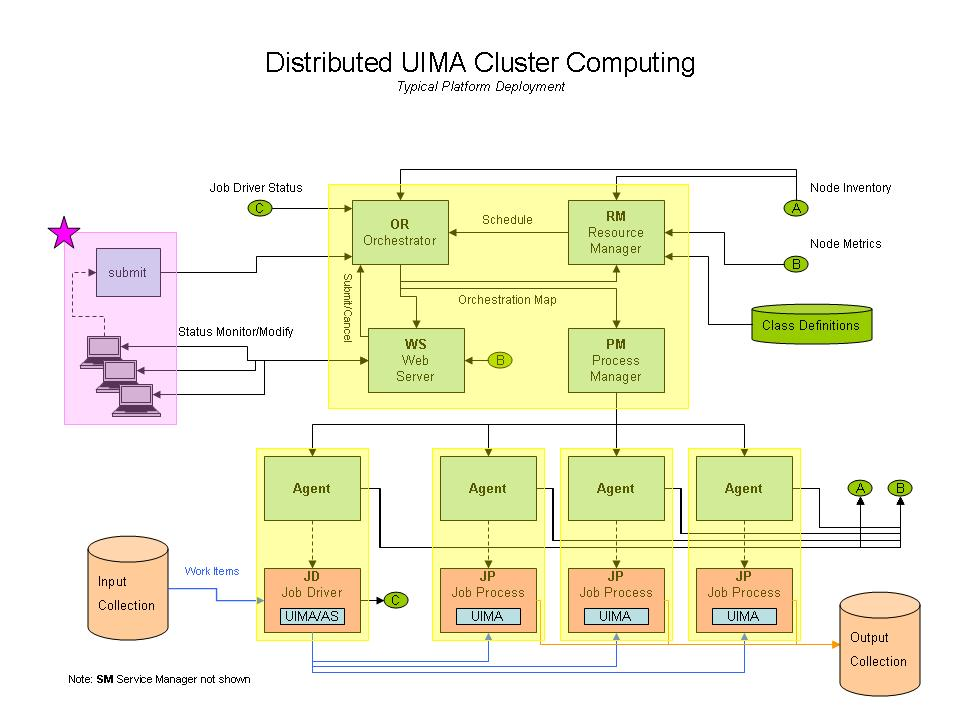
\includegraphics[width=6.5in]{images/ducc-arch.jpg}
      \label{fig:DUCC-Architecture}
    \end{figure}
    
%    \begin{figure}[h]
%    \centering
%    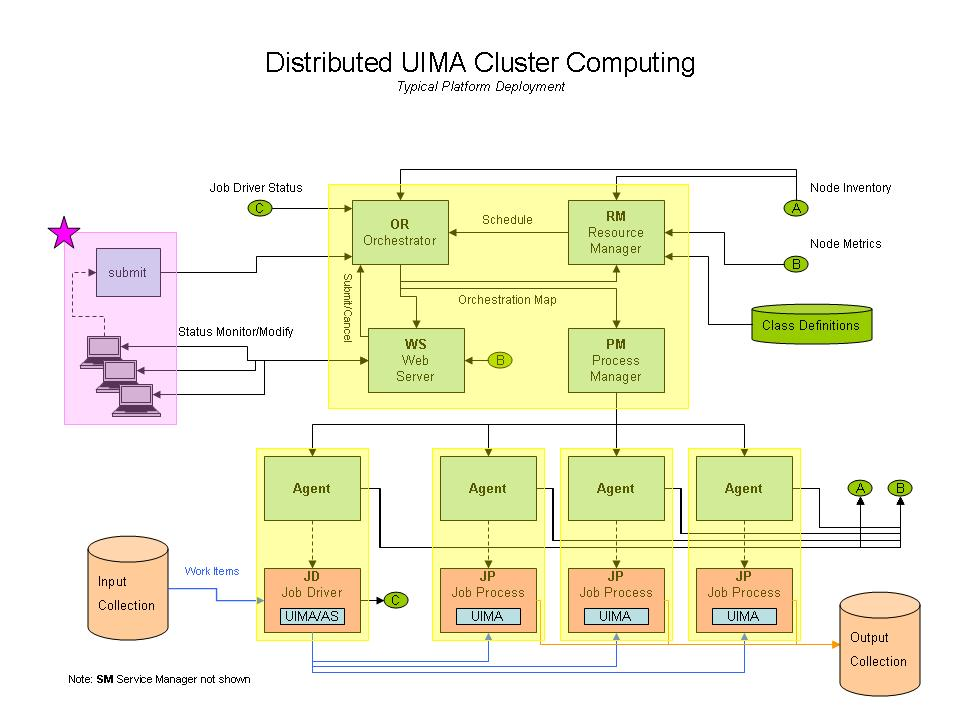
\includegraphics[width=6.5in]{images/ducc-arch.jpg}
%    \caption[]{\varDUCC~Architecture}
%    \label{fig:\varDUCC~Architecture}
%    \end{figure}
%    \label{fig:01}

    \section{\varJobs}

    The main focus of the system is running "batch" \varJobs~comprising \varUIMA~pipelines.
    
    Users submit \varJobs~to the system to be deployed and executed. \varJobs~have a
    life-cycle from birth to death during which time a (normally) finite collection of
    work items are processed by one or more \varUIMA~pipelines. \varJobs~consist of two
    parts: a singleton work item supplier, known in \varUIMA~parlance as a
    \varCollectionReader~(\varCR); and one or more pipelines, each known in \varUIMA~parlance
    as an \varAnalysisEngine~(\varAE).
        
    \subsection{Characteristics}   
    
    \varDUCC~facilitates "fair-share" \varUIMA~pipeline scale-out.
    
    The \varUIMA~pipelines comprising a \varJob~represent "embarrassingly parallel" 
    deployments. Over time, a \varJob~may expand and contract with respect to the number of 
    \varUIMA~pipelines deployed during its lifetime. This may be due to the introduction 
    or completion of other \varJobs, the rise and fall of other resource consumers such 
    as \varReservations~or \varServices, and the addition or removal of computer resources 
    to the cluster.
    
    With respect to contraction, each \varUIMA~pipeline must be prepared to
    process work items that may have been partially processed previously.
   
    Pipelines themselves may comprise one or more duplicate threads, such that each
    pipeline can simultaneously process multiple work items.
    The number of pipelines and threads per pipeline are configurable per \varJob.
   
    \subsection{Performance}  
    
    For the distributed environment, \varDUCC~relies upon a \varNetworkFileSystem~(\varNFS)
    for file access to work items.
    High performance is achieved through \varNFS~data sharing and (via \varActiveMQ) the passing of
    data-handles that are utilized by the "embarrassingly parallel" pipelines.
    
    \section{\varReservations}
    
    To help support Jobs, \varDUCC~provides facilities for \varReservations~of two types: 
    Managed and Unmanaged. \varReservations, once allocated, are preserved until 
    canceled. 
    
    \varManagedReservations~(MRs) comprise "arbitrary" processes, for example Java
    programs, c-programs, bash shells, etc.
    
    \varUnmanagedReservations~(URs) comprise a resource that can be utilized for any 
    purpose, subject to the limitations of the assigned \varShare~or \varShares.
            
    \section{\varServices}
       
    To help support \varJobs, \varDUCC~provides facilities for \varServices~of two types: 
    \varUIMA~and \varPingOnly. \varServices~can be predefined in a registry, and 
    \varJobs~can declare dependency on one or more of them.
    
    \varServices~can be shared by my multiple \varJobs~or can be tied to just one.
    \varServices~can be started at \varDUCC-boot time or at \varService-definition time or
    at \varJob~launch time.
    
    \varServices~can be expanded and contracted by command or on-demand.  
    \varServices~can be stopped by command or due to absence of demand.
    
    \varServices~nominally exists for reasons of efficiency due to high start-up costs
    or high resource consumption.  Benefits of cost amortization are realized by sharing
    \varServices~amongst a collection of \varJobs~rather than employing a private copy 
    for each.
    
    The lifecycle of each \varUIMA~\varService~is managed by \varDUCC, which is not the
    case for \varPingOnly~\varServices.  However, each comprises a "pinger" which 
    adheres to a standard interface and provides health and statistical information.
    
    \section{Management} 
    
    The \varDUCC~system employs several management techniques to fairly apportion
    resources.
    
    \subsection{Memory Shares} 
    
    The \varDUCC~system partitions the entire set of available resources comprising
    \varNodesMachinesComputers~into \varShares.
    
    Partitioning of the available \varNodesMachinesComputers~into \varShares~facilitates
    multitenancy amongst a collection of \varDUCC-managed user applications consisting 
    of \varUIMA~pipelines.
    
    One or more \varShares~are allocated and sub-partitioned into \varJdShares.
    
    Users submit \varJobs~to the \varDUCC~system specifying a requisite memory size.
    Each \varJob~is allocated one \varJdShare~and, based upon user specified
    memory size, one or more \varShares. 
    Likewise, users submit \varReservations~and \varServices~also comprising memory size
    information.  These are assigned \varShares~only.
    
    New \varJobs, \varReservations~and \varServices~may only enter the system when
    there are sufficient unallocated \varShares~available. To make room for newly arriving
    submissions, the \varResourceManager~may preempt use of already previously
    assigned \varShares~for re-assignment.
    
    \subsection{\varLinuxControlGroups} 
    
    If available, \varDUCC~employs \varLinuxControlGroups~to enforce limits on
    deployed applications. Exceeding limits penalizes only the offender.
    For example, if a user application exceeds its memory \varShare~size then it is forced
    to swap while other co-resident applications remain unaffected.
    
    \subsection{Preemption} 
        
    Preemption is employed by \varDUCC~to re-apportion \varShares~when new work is submitted.
    
    For example, presume a simple \varDUCC~system with just one preemptable scheduling class
    and resources comprising 11 \varShares. Further, suppose that 1 \varShare~is allocated 
    for partitioning into \varJdShares.
    When the Job \#1 is submitted it is entitled to all remaining 10 shares.  
    When Job \#2 arrives, each job is entitled to only 5 shares.
    Thus, 5 \varShares~from Job \#1 are preempted and reassigned to Job \#2.
    
\chapter{System Organization}

    \section{Single System Image}
    
    \varDUCC~runs on \varLinux. It can be run on a single system in simulation-mode
    or on a cluster (two or more machines). For clusters, \varDUCC~replies upon 
    these requirements:
    
    \begin{itemize}
      \item common userids across the cluster
      
      Each userid must have the same definition on all machines participating
      in the \varDUCC~cluster.
      
      \item a shared filesystem for user and \varDUCC~data across the cluster
      
      Each machine shares a filesystem (commonly provided by NFS) with all 
      machines participating in the \varDUCC~cluster.
      
    \end{itemize} 
    
    \section{Communications}
    
    \varDUCC~comprises a collection of singleton and distributed daemons that need
    to coordinate activities.  This coordination is accomplished via messaging.
    
    The system is fault tolerant with respect to lost messages, since
    publications occur at regular intervals and each message encapsulates
    the current and/or desired state for the target audience.
    As such, actions may be be delayed but will be carried out as soon as the
    next message arrives.
    
    \section{Daemons}
    
    \varDUCC~is implemented through a collection of configurable singleton 
    and distributed daemons.
    
    % 
% Licensed to the Apache Software Foundation (ASF) under one
% or more contributor license agreements.  See the NOTICE file
% distributed with this work for additional information
% regarding copyright ownership.  The ASF licenses this file
% to you under the Apache License, Version 2.0 (the
% "License"); you may not use this file except in compliance
% with the License.  You may obtain a copy of the License at
% 
%   http://www.apache.org/licenses/LICENSE-2.0
% 
% Unless required by applicable law or agreed to in writing,
% software distributed under the License is distributed on an
% "AS IS" BASIS, WITHOUT WARRANTIES OR CONDITIONS OF ANY
% KIND, either express or implied.  See the License for the
% specific language governing permissions and limitations
% under the License.
% 
    
    \subsection{\varOrchestrator~(\varOR)} 
    
    There is one \varOrchestrator~per \varDUCC~cluster.
    
    The duties of the \varOrchestrator~are:
    \textit{
      % 
% Licensed to the Apache Software Foundation (ASF) under one
% or more contributor license agreements.  See the NOTICE file
% distributed with this work for additional information
% regarding copyright ownership.  The ASF licenses this file
% to you under the Apache License, Version 2.0 (the
% "License"); you may not use this file except in compliance
% with the License.  You may obtain a copy of the License at
% 
%   http://www.apache.org/licenses/LICENSE-2.0
% 
% Unless required by applicable law or agreed to in writing,
% software distributed under the License is distributed on an
% "AS IS" BASIS, WITHOUT WARRANTIES OR CONDITIONS OF ANY
% KIND, either express or implied.  See the License for the
% specific language governing permissions and limitations
% under the License.
% 
\begin{description}
  \item receive and act upon user submitted application requests;
  \item manage and publish common state to a set of distributed components;
  \item maintain checkpoint and historical state;
  \item manage the lifecycle of jobs, services, and reservations.
\end{description}
    }
    
    The \varOrchestrator~provides essential functionality for operation of the
    \varDUCC~system.
    It is configurable and tunable.
    
    The \varOrchestrator~receives user requests to start, stop and modify 
    Jobs, Services and Reservations. It manages the life-cycles of these
    entities, each deployed to a managed cluster of machines 
    (nodes, computers).
    
    The \varOrchestrator~both publishes and receive reports.  
    The \varOrchestrator~publication is also known as the \varORmap, which is
    the final authority on the state of Jobs, Reservations, and Services.
    All other \varDUCC~components respect the state published by the 
    \varOrchestrator~and each carries out its assigned duties accordingly.
    
    \subsubsection{Controller} 
    \label{Controller}
    
    The \varOrchestrator~Controller responsibilities entail receiving user 
    submitted requests and processing them to completion in accordance with 
    an instance of the appropriate state machine. 
    
    User submitted requests comprise:
    
    \begin{itemize}
      \item Job \{ Start, Stop, Modify \}
      \item Reservation \{ Start, Stop, Modify \}
      \item Service \{ Start, Stop, Modify \}
      \item Individual Process \{ Stop \}
    \end{itemize} 
    
    The Controller responsibilities further entail receiving status messages
    from other \varDUCC~components and advancing the state machines of user 
    submitted Jobs, Reservations, and Services as necessary. 
    
    Additionally and importantly, the Controller is the final authority
    for the \varDUCC~system state comprising active Jobs, Reservations, and 
    Services. The Controller publishes \varDUCC~system state at regular intervals
    for consumption and use by all other \varDUCC~components.
    
    \subsubsection{Authenticator} 
    
    The authenticator determines whether or not the requesting user is a
    \varDUCC~administrator. Such users have special privileges, such as:
    
    \begin{itemize}
      \item the ability to control \varDUCC~system functions
      \item the ability to act on behalf of other users
    \end{itemize}     
    
    The file \varDuccAdministrators~comprises the list of privileged \varDUCC~users.
    
    \subsubsection{Validation} 
    
    Each request to submit, cancel or modify is validated against a set of
    criteria that define acceptableness. In the case of missing information,
    a default value may be employed.
    
    Presently, the following keys are validated by the \varOrchestrator:
    
    \begin{itemize}
      \item \varProcessThreadCount
      \item \varNumberOfInstances
      \item \varSchedulingClass
    \end{itemize} 
    
    Other keys are validated by the \varCommandLineInterface, prior to arrival
    at the \varOrchestrator.
    
    \subsubsection{Factory} 
    
    Once accepted, submit requests proceed through a corresponding factory
    to have a state machine representation entered into the published
    \varORmap~with initial state of \varReceived.  The request remains 
    active until it advances to final state \varCompleted.
    
    Each factory-created representation comprises appropriate information as follows:
    
    \begin{itemize}
      \item

      \begin{itemize}
      \item standard information
        \begin{itemize}
          \item unique identifier (assigned by \varDUCC)
          \item type {Job, Reservation, Service}
          \item user name
          \item submitting \varPID
          \item date of submission
          \item date of completion (initially \varNull)
          \item description (text supplied by user)
        \end{itemize} 



      \item scheduling information
        \begin{itemize}
          \item scheduling class
          \item scheduling priority
          \item scheduling max shares
          \item scheduling min shares
          \item scheduling threads per share
          \item scheduling memory size
          \item scheduling memory units
        \end{itemize} 
      \item job driver information
        \begin{itemize}
          \item java command
          \item java classpath
          \item environment variables
          \item user log directory
          \item MQ broker
          \item MQ queue
          \item \varCollectionReader~descriptor
          \item \varCollectionReader~overrides
          \item getMeta timeout value
          \item work item processing timeout value
          \item work item processing exception handler
          \item node identity
          \item \varLinuxControlGroup~limits
          \item state
        \end{itemize} 
      \item job process information (one or more instances)
        \begin{itemize}
          \item java command
          \item java classpath
          \item environment variables
          \item user log directory
          \item MQ broker
          \item MQ queue
          \item deployment descriptor or aggregate data
          \item initialization failure limits
          \item node identity
          \item \varLinuxControlGroup~limits
          \item state
          \item service dependencies
        \end{itemize} 
      \item service information (one or more instances)
        \begin{itemize}
          \item See job process information above.
        \end{itemize} 

      \item managed reservation information
        TBD      
      \item unmanaged reservation information
        TBD          

    \end{itemize} 
  \end{itemize}    


  \subsubsection{Checkpoint Supervisor} 
    
    The Checkpoint Supervisor provides functions to save and restore state information
    to/from persistent storage. State is stored whenever a significant change occurs.
    State is restored at \varOrchestrator~boot time.
    
    Saving and restoration of state facilitates reasonable continuity of service
    between \varOrchestrator~lifetimes.
    
    \subsubsection{State Supervisor} 

    The State Supervisor receives and examines publications from other
    \varDUCC~components, records and distributes pertinent information obtained
    or derived, and advances state machines appropriately.
    
    Publications are received from these components:
    
    \begin{itemize}
    
    \item Job Driver(s)
    \item Resource Manager
    \item Services Manager
    \item Agent(s) Inventory
      
    \end{itemize} 
    
    Information from these sources is recorded in the \varORmap. 
    Based on information derived from all sources, the 
    \varOrchestrator~advances the state machines of currently active 
    entities (Jobs, Reservations, Services). 
    Once the \varCompleted~state is reached, the
    entity is no longer active on the cluster.
    
    Note that \varORmap~is, in-turn, published at regular intervals 
    for use by the other \varDUCC~singleton and distributed components.
    The \varORmap~is the "final authority" on the state of
    each Job, Reservation and Service currently or formerly deployed.
    See \ref{Controller} \varController.
    
    \subsubsection{State Accounting Supervisor} 
        
    The State Accounting Supervisor manages finite state machine for 
    Jobs, Services, and Reservations. It provides functions to:
    
    \begin{description}
    
    \item Advance from the current state to a next valid state
    \item Advance from the current state immediately to the \varCompleted~state
          
    \end{description} 
    
    \subsubsection{\varLinuxControlGroup~Supervisor}  
    
    The \varLinuxControlGroup~Supervisor assigns a maximum size (in bytes) and a composite
    unique identity to each \varShare. This information is published for use
    by Agents to enforce \varLinuxControlGroup~limitations on storage used by the corresponding
    running entity (for example, \varUIMA~pipeline).
    
    Employing \varLinuxControlGroups~ is analogous to defining virtual machines of a certain
    size such that exceeding limits causes only the offending process to suffer
    any performance penalties, while other co-located well-behaved processes
    run unaffected.
    
    \subsubsection{Host Supervisor}
    
    The Host Supervisor is responsible for obtaining sufficient resource for
    deploying the Job Drivers for all submitted Jobs. It interacts with the
    Resource Manager to allocate and de-allocate resources for this purpose.
    It assigns a \varJdShare~to each active Job.
    
    A \varJdShare~is a \varLinuxControlGroup~controlled \varShare~of sufficient size into which a Job
    Driver can be deployed.  A \varJdShare~is usually significantly smaller than
    a normal \varShare.
    
    \subsubsection{Logging / As-User} 
    
    The Logging and As-User modules permit the \varOrchestrator~to write logging data into
    a file contained in "user-space", meaning a file into a directory writable 
    by the submitting user, during processing of the submitted entity 
    (Job, Managed Reservation...).
    
    The Logging module also facilitates the recording to persistent storage of noteworthy
    events occurring during the \varOrchestrator~lifetime. Noteworthiness is configurable
    as various levels, such as \varINFO, \varDEBUG~and \varTRACE.
        
    \subsubsection{Administrators} 
    
    The Administrators module grants users defined in the \varDuccAdministrators~file
    special privileges, such a being able cancel to any user's Job.
    
    \subsubsection{Maintenance} 
    
    The maintenance thread wakes-up at regular intervals to perform the following
    tasks:
    
    \begin{description}
    
      \item Health
      
      The \varOrchestrator~automatically caps Jobs and Services that exceed initialization
      error thresholds, and cancels those that exceed processing error thresholds.
      
      \item MQ Reaper
      
      The \varOrchestrator~cleans-up unused \varJobDriver~AMQ permanent queues for Jobs that have completed.
      
      \item Publication Pruning
      
      The \varOrchestrator~regularly publishes state for all active entities (Jobs, Reservations,
      Services).  It also publishes state for recently completed ones. Pruning removes
      from regular \varOrchestrator~publication completed entities that have been competed past a
      time threshold, nominally one minute.
           
      \item Node Accounting
      
      This module keeps track of each node's state, up or down.  Nodes that do 
      not report for a time exceeding a threshold, typically a few minutes, 
      are considered down. This information is used for Jobs whose Job Driver
      advanced to the \varCompleted~state, whereby corresponding Job Processes on 
      nodes that are reported down are marked as stopped by the \varOrchestrator, as opposed 
      to waiting (potentially forever) for the corresponding Agent to report.
      This prevents Jobs from becoming unnecessarily stuck in the completing
      state.
      
    \end{description} 
    

    % 
% Licensed to the Apache Software Foundation (ASF) under one
% or more contributor license agreements.  See the NOTICE file
% distributed with this work for additional information
% regarding copyright ownership.  The ASF licenses this file
% to you under the Apache License, Version 2.0 (the
% "License"); you may not use this file except in compliance
% with the License.  You may obtain a copy of the License at
% 
%   http://www.apache.org/licenses/LICENSE-2.0
% 
% Unless required by applicable law or agreed to in writing,
% software distributed under the License is distributed on an
% "AS IS" BASIS, WITHOUT WARRANTIES OR CONDITIONS OF ANY
% KIND, either express or implied.  See the License for the
% specific language governing permissions and limitations
% under the License.
% 

    \subsection{\varResourceManager~(\varRM, also known as the \varScheduler)}    
        
    There is one \varResourceManager~per \varDUCC~cluster.
    
    The duties of the \varResourceManager~are:
    \textit{
      % 
% Licensed to the Apache Software Foundation (ASF) under one
% or more contributor license agreements.  See the NOTICE file
% distributed with this work for additional information
% regarding copyright ownership.  The ASF licenses this file
% to you under the Apache License, Version 2.0 (the
% "License"); you may not use this file except in compliance
% with the License.  You may obtain a copy of the License at
% 
%   http://www.apache.org/licenses/LICENSE-2.0
% 
% Unless required by applicable law or agreed to in writing,
% software distributed under the License is distributed on an
% "AS IS" BASIS, WITHOUT WARRANTIES OR CONDITIONS OF ANY
% KIND, either express or implied.  See the License for the
% specific language governing permissions and limitations
% under the License.
% 
\begin{description}
  \item fairly allocate constrained resources amongst valid user requests over
  time.
\end{description}
    }
    
    The \varResourceManager~provides essential functionality for operation of the
    \varDUCC~system.
    It is configurable and tunable.
    It is also plug-replaceable.
    
    The \varResourceManager~both publishes and receive reports.  
    The \varResourceManager~receives \varOrchestrator~publications comprising
    Jobs, Reservations, and Services as well as 
    \varAgent~publications comprising inventory and metrics. 
    The \varResourceManager~publication occurs at regular intervals, each
    representing at the time of its publication the desired allocation
    of resources. 
   
    The \varResourceManager~considers various factors to make assignments, including:
    \begin{description}
      \item supply of available nodes;
      \item memory size of each available node;
      \item demand for resource in terms of memory size and class of service comprising Jobs, Reservations and Services;
      \item the most recent previous assignments and desirability for continuity;
    \end{description}
    
    The \varOrchestrator~is the primary consumer of the \varResourceManager~publication
    which it uses to bring the cluster into compliance with the allocation assignments.
    
    The \varResourceManager~adheres to the \varIScheduler~interface. 
    Algorithms adhering to this interface are eligible for replacing
    the \varDUCC~supplied one.
    
    \subsubsection{Job Manager Converter} 
    
    The Job Manager Converter module receives \varOrchestrator~publications and
    updates its internal state with new, changed, and removed map entries
    comprising Jobs, Reservations and Services.
        
    \subsubsection{Node Stability}
    
    The Node Status module evaluates the health of the nodes within the cluster
    for consideration during resource scheduling.  Any node deemed unhealthy is
    removed from the collection of available resources until such time as it
    is once again deemed healthy.
      
    \subsubsection{Node Status} 
        
    The Node Status module receives \varAgent~publications and
    updates its internal state with new, changed, and removed node status entries.
     
    \subsubsection{Resource Manager} 
    
    The \varResourceManager~performs the following:
    
    \begin{description}
      \item receive resource availability reports from \varAgents;
      \item receive resource need requests the \varOrchestrator;
      \item employ a scheduling algorithm at discrete time intervals to:
      \begin{description}
        \item consider the resource supply;
        \item consider the most recent allocation set;
        \item consider new, changed and removed resource demands;
        \item assign a resource to a request;
        \item remove a resource from a request;
        \item publish current allocation set;
      \end{description} 
    \end{description}     
        
    \subsubsection{\varScheduler} 
    
    The \varScheduler~runs at discrete time intervals.
    It assembles information about available nodes in the cluster.
    Each node, based upon its memory size is partitioned into zero or more \varShares.
    Each request (Job, Reservation and Service) is assessed as to the number of
    \varShares~required based upon user-specified memory size. 
    In addition, each request is assessed with respect to the user-specified class-of-service.

    The \varScheduler~considers the most recent previous allocations along with changes
    to supply and demand.  It then produces a new allocation set which the 
    \varResourceManager~publishes as directions to the \varOrchestrator.
    
    % 
% Licensed to the Apache Software Foundation (ASF) under one
% or more contributor license agreements.  See the NOTICE file
% distributed with this work for additional information
% regarding copyright ownership.  The ASF licenses this file
% to you under the Apache License, Version 2.0 (the
% "License"); you may not use this file except in compliance
% with the License.  You may obtain a copy of the License at
% 
%   http://www.apache.org/licenses/LICENSE-2.0
% 
% Unless required by applicable law or agreed to in writing,
% software distributed under the License is distributed on an
% "AS IS" BASIS, WITHOUT WARRANTIES OR CONDITIONS OF ANY
% KIND, either express or implied.  See the License for the
% specific language governing permissions and limitations
% under the License.
% 
    
    \subsection{\varServicesManager~(\varSM)}    
    
    There is one \varServicesManager~per \varDUCC~cluster.
    
    The duties of the \varServicesManager~are:
    \textit{
      % 
% Licensed to the Apache Software Foundation (ASF) under one
% or more contributor license agreements.  See the NOTICE file
% distributed with this work for additional information
% regarding copyright ownership.  The ASF licenses this file
% to you under the Apache License, Version 2.0 (the
% "License"); you may not use this file except in compliance
% with the License.  You may obtain a copy of the License at
% 
%   http://www.apache.org/licenses/LICENSE-2.0
% 
% Unless required by applicable law or agreed to in writing,
% software distributed under the License is distributed on an
% "AS IS" BASIS, WITHOUT WARRANTIES OR CONDITIONS OF ANY
% KIND, either express or implied.  See the License for the
% specific language governing permissions and limitations
% under the License.
% 
\begin{description}
  \item facilitate services definition and persistence;
  \item monitor and control services as dependencies on-demand.
\end{description}
    }
        
    The \varServicesManager~provides additional functionality for operation of the
    \varDUCC~system.
    It is configurable and tunable.
    
    Although not essential for the main purpose of the \varDUCC~system, in
    practical terms for large systems the \varServicesManager~is highly 
    desirable for improved resource utilization.
    By using shared services, resources are more effectively employed and
    work items processing is completed sooner.
    
    Some dimensions:
    
    \begin{itemize}
    
      \item long warm-up time
      
      When the service takes a long time to warm-up, the \varJob~in progress
      may have to sit idle for a long time before the first work item can be
      processed until the service upon which it depends has initialized and 
      is ready.
      If the service is already up and ready, this delay can be avoided
      and the \varJob~experiences no service delay.
      
      \item large storage use
      
      When the service has a large memory footprint, it can be far more
      efficient to have multiple \varJobs~share the service rather than
      having separate copies for each.
      
      \item short processing time
      
      Related to large storage use, if the time to process a work item is
      relatively short, again it can be much more efficient to share the
      service amongst multiple \varJobs.
      
      \item not used
      
      If a service has not been used for a relatively long time, it may be 
      better to shut it down and reclaim the resources for use elsewhere, 
      especially on a busy cluster.
            
    \end{itemize}
    
    \subsubsection{Ping Driver} 
    
    This runs the watchdog thread for custom service pingers.
    It ascertains the liveness and healthiness of each service
    known to \varDUCC.
    
    \subsubsection{Service Handler} 
    
    Carries out Service Manager validated request operations.
            
    \subsubsection{Service Manager, API Handler} 
    
    Receives and validates service request operations:
    
    \begin{itemize}
      \item register
      \item unregister
      \item start
      \item stop
      \item query
      \item modify
    \end{itemize}
    
    The \varServicesManager~maintains a registry of services.
    The attributes of these services may include one of more of the following:
    
    \begin{description}
      \item \texttt{permanent}
      A permanent service is one that is kept up so long as the
      \varDUCC~system is running.
      \item \texttt{on-demand}
      An on-demand service is one that is kept up only during the
      lifetime of one or more \varJobs~that declare a dependency on the 
      service
      \item \texttt{lingering}
      A lingering service is one that continues for some limited time
      beyond the lifetime of the last dependent \varJob~in anticipation
      of another \varJob~arrival in the near future.
      \item \texttt{dynamic}
      A dynamic service is one that automatically expands and contracts
      in terms of number of instances to meet demand.
      \item \texttt{registered}
      A registered service is one that is pre-defined, whose definition
      is kept persistently and whose lifecycle is managed by \varDUCC.
      \item \texttt{custom}
      A custom (unregistered) service is one that is not pre-defined, whose definition
      is not kept persistently and whose lifecycle is not managed by \varDUCC.
    \end{description}
  
    The \varServicesManager~keeps within its registry information of
    two types: \texttt{service} and \texttt{meta}.
    
    Type \texttt{service} information includes the following attributes:
    \begin{itemize}
      \item classpath
      \item description
      \item environment
      \item jvm
      \item jvm args
      \item log directory
      \item deployment descriptor
      \item failures limit
      \item memory size
      \item scheduling class
      \item linger time
      \item pinger classpath
      \item pinger log
      \item pinger timeout
      \item service endpoint
      \item working directory
    \end{itemize}
    
    Type \texttt{meta} information includes the following attributes:
    \begin{itemize}
      \item autostart
      \item endpoint
      \item implementors
      \item instances (count)
      \item identifier (number)
      \item ping-active
      \item ping-only
      \item service-active
      \item service-class
      \item service-health
      \item service-state
      \item service-statistics
      \item service-type
      \item stopped
      \item user
      \item uuid
      \item work-instances (PID list)
    \end{itemize}
    
    % 
% Licensed to the Apache Software Foundation (ASF) under one
% or more contributor license agreements.  See the NOTICE file
% distributed with this work for additional information
% regarding copyright ownership.  The ASF licenses this file
% to you under the Apache License, Version 2.0 (the
% "License"); you may not use this file except in compliance
% with the License.  You may obtain a copy of the License at
% 
%   http://www.apache.org/licenses/LICENSE-2.0
% 
% Unless required by applicable law or agreed to in writing,
% software distributed under the License is distributed on an
% "AS IS" BASIS, WITHOUT WARRANTIES OR CONDITIONS OF ANY
% KIND, either express or implied.  See the License for the
% specific language governing permissions and limitations
% under the License.
% 
    
    \subsection{\varProcessManager (\varPM)}    
    
    There is one \varProcessManager~per \varDUCC~cluster.
    
    The duties of the \varProcessManager~are:
    \textit{
      % 
% Licensed to the Apache Software Foundation (ASF) under one
% or more contributor license agreements.  See the NOTICE file
% distributed with this work for additional information
% regarding copyright ownership.  The ASF licenses this file
% to you under the Apache License, Version 2.0 (the
% "License"); you may not use this file except in compliance
% with the License.  You may obtain a copy of the License at
% 
%   http://www.apache.org/licenses/LICENSE-2.0
% 
% Unless required by applicable law or agreed to in writing,
% software distributed under the License is distributed on an
% "AS IS" BASIS, WITHOUT WARRANTIES OR CONDITIONS OF ANY
% KIND, either express or implied.  See the License for the
% specific language governing permissions and limitations
% under the License.
% 
\begin{description}
  \item monitor and control processes supporting analytic pipelines distributed
  over a collection of agent-managed nodes.
\end{description}
    }
      
    The \varProcessManager~provides essential functionality for operation of the
    \varDUCC~system.
    
    The \varProcessManager~both publishes and receive reports.  
    The \varProcessManager~receives \varOrchestrator~publications comprising
    Jobs, Reservations, and Services.
    The \varProcessManager~distributes two publications at regular intervals.
    One is heartbeat information to notify the \varOrchestrator~and
    \varWebServer~that the \varProcessManager~is alive.  
    The other is compacted \varAgent-destined information regarding
    processes that need to be started, stopped or modified.
    
    The main function of the \varProcessManager~is to efficiently manage
    the distributed \varAgents~each of which manages processes running
    locally on its own respective \varNodeMachineComputer.
    The \varProcessManager~interprets the \varOrchestrator~publications and 
    redistributes only the essentials to the collection of distributed
    \varAgents~who each independently act to bring the 
    state of locally deployed processes into compliance.  
    % 
% Licensed to the Apache Software Foundation (ASF) under one
% or more contributor license agreements.  See the NOTICE file
% distributed with this work for additional information
% regarding copyright ownership.  The ASF licenses this file
% to you under the Apache License, Version 2.0 (the
% "License"); you may not use this file except in compliance
% with the License.  You may obtain a copy of the License at
% 
%   http://www.apache.org/licenses/LICENSE-2.0
% 
% Unless required by applicable law or agreed to in writing,
% software distributed under the License is distributed on an
% "AS IS" BASIS, WITHOUT WARRANTIES OR CONDITIONS OF ANY
% KIND, either express or implied.  See the License for the
% specific language governing permissions and limitations
% under the License.
% 
    
    \subsection{\varAgent}  

    There is one \varAgent~per~\varNodeMachineComputer~per \varDUCC~cluster.
    The \varAgents~collectively provide essential functionality for operation
    of the \varDUCC~system.
    
    The duties of the \varAgent~are:
    \textit{
      % 
% Licensed to the Apache Software Foundation (ASF) under one
% or more contributor license agreements.  See the NOTICE file
% distributed with this work for additional information
% regarding copyright ownership.  The ASF licenses this file
% to you under the Apache License, Version 2.0 (the
% "License"); you may not use this file except in compliance
% with the License.  You may obtain a copy of the License at
% 
%   http://www.apache.org/licenses/LICENSE-2.0
% 
% Unless required by applicable law or agreed to in writing,
% software distributed under the License is distributed on an
% "AS IS" BASIS, WITHOUT WARRANTIES OR CONDITIONS OF ANY
% KIND, either express or implied.  See the License for the
% specific language governing permissions and limitations
% under the License.
% 
\begin{description}
  \item deploy, monitor and control one or more  processes supporting analytic
  pipelines on one node; and
  \item publish inventory and metrics.
\end{description}
    }
 
    At the direction of the \varProcessManager, each \varAgent~is
    instructed to manage its assigned \varShares~by means of
    \varLinuxControlGroups, and by injecting into them local 
    process elements comprising
    Job Drivers, Job Processes, Service Processes, and Managed Processes.
    
    The \varAgent~is subdivided into several responsibility areas:

    \begin{itemize}
      \item Core
      \item Config
      \item Deploy
      \item Event
      \item Exceptions
      \item Launcher
      \item Metrics Collectors
      \item Monitor
      \item Processors
    \end{itemize}
                     
    \subsubsection{Core}    
    
    The \varAgent~publishes information about the state of the
    \varNodeMachineComputer~it controls.
    It also receives publications which it interprets to control
    processes deployed thereon.
    It also monitors activity on the \varNodeMachineComputer~and
    ensures that only sanctioned processes are running.
    
    The \varAgent~is normally launched at \varDUCC~system
    start-up time.
    However, \varAgents~may be started/stopped independently over time.
    
    \varDUCC~is only able to deploy user submitted applications to a
    \varNodeMachineComputer~upon which there exists an active \varAgent.
    
    \subsubsection{Config}     
    
    \begin{itemize}
      \item Agent Configuration
      
      The \varAgent configures itself according to the 
      \varDuccProperties~file.  Aspects include:
      
      \begin{itemize}
        \item launcher.thread.pool.size
        \item launcher.process.stop.timeout
        \item rogue.process.exclusion.filter
        
        Processes in this list are exempt for rogue process detection
        and termination.
        
        \item rogue.process.user.exclusion.filter
        
        Users in this list are exempt for rogue process detection
        and termination.
        
      \end{itemize} 
      
      The \varAgent publishes reports at configurable intervals:
      
      \begin{itemize}
        \item Node Inventory
        
        Node Inventory is a report on the \varAgent-managed processes
        on this node.
        
        \item Node Metrics
        
        Node Metrics is a report on the \varAgent-observed metrics
        on this node.
        
      \end{itemize} 
      
    \end{itemize}  
            
    \subsubsection{Deploy}
    
    \begin{itemize}
      \item Managed UIMA Service
      
      The module is the \varAgent-managed integration between
      \varUIMAAS~and the user supplied application code which is
      deployed thereto.
      
    \end{itemize}    
    
    \subsubsection{Event}  
    
    \begin{itemize}
      \item Event Listener
      
      The module handles publication events:
      \begin{itemize}
      \item Process Start 
      
      A notification from the \varProcessManager~to start a user submitted 
      process constrained to a \varResourceManager~allocated number of \varShares.
      
      \item Process Stop
      
      A notification from the \varProcessManager~to stop a user submitted 
      process.
      
      \item Process Modify
            
      A notification from the \varProcessManager~to modify a user submitted 
      process.
      
      \item Process Purge
                  
      A notification from the \varProcessManager~to purge a user submitted 
      process.
      
      \item Job State
                        
      A notification from the \varProcessManager~comprising abbreviated
      state of the \varDUCC-managed collection of entities: 
      \varJobs, \varReservations~and \varServices.
      
      \end{itemize}  

    \end{itemize}     
                 
    \subsubsection{Launcher}   
          
    The modules comprising the Launcher package are tasked with
    starting user processes on the \varAgent-managed \varNodeMachineComputer.
    The modules are:
            
    \begin{itemize}
      \item CGroups Manager
      
      This module provides functionality to partition the \varAgent-managed
      \varNodeMachineComputer~into \varShares, each \varShare~with limits on one
      or more aspects, including but not limited to memory and swap space. 
      
      The CGroups Manager essentially starts, maintains, and stops instant
      virtual machines in correspondence with \varResourceManager~allocated
      \varShares~into which user submitted processes are launched.
      
      \item Command Executor
      
      This module is the base class that provides functionality to
      launch a user specified process within the 
      \varResourceManager~allocated \varShare. 
      
      \item \varDUCC~Command Executor
      
      This module launches a user specified process within the 
      \varResourceManager~allocated \varShare. 
      The process may be constrained by a \varLinuxControlGroup~and
      may be spawned as the submitting \varUser.
      
      \item \varJVM~Args Parser
      
      The \varJVM~Args Parser module extracts user specified \varJVM~arguments
      for use in building an \varAgent-launchable subprocess comprising
      the user specified executable code.
      
      \item Launcher
      
      The Managed Process module provides virtual \varAgent~capability.
      
      This module comprises a method used to launch multiple Agents
      on the same physical machine. 
      It allows for the scale up Agents on a single machine to simulate load.
      Each Agent instance assumes a given name and IP address.
      
      \item Managed Process

      The Managed Process module manages a state machine for each
      \varAgent-managed user process.  The states comprise:
      
         \begin{itemize}
           \item Starting
           \item Initializing
           \item Ready
           \item Failed
           \item Stopped
         \end{itemize}
         
      \item Process Stream Consumer
      
      The Process Stream Consumer module captures and redirects user process output
      to a log file.
      
    \end{itemize}  
    
    \subsubsection{Metrics Collectors} 
    
    The modules comprising the Metrics Collectors package observe, calculate
    or otherwise gather specific metrics. Metrics collected are relative to
    these main categories:
        
    \begin{itemize}
      \item Garbage Collection Statistics
      \item Node CPU, Node CPU Usage, Node CPU Utilization
      \item Node Load Average
      \item Node Memory Info
      \item Node Users
      \item Process CPU Usage
      \item Process Major Faults
      \item Process Resident Memory
      \item Process Swap Usage
    \end{itemize}  
    
    \subsubsection{Monitor} 

    The modules comprising the Monitor package observe various states and
    trigger actions when specific events occur.
        
    \begin{itemize}
      \item \varAgent~Monitor
      
      When the \varAgent~detects problems with the network, broker, or ping
      functions it terminates all \varAgent~deployed processes.
       
      \item Rogue Process Detector
      
      The \varAgent~detects aliens processes, those not expected for running
      the \varOS~or \varDUCC~or user processes deployed by \varDUCC.
      According to policy, the \varAgent~may take one or more actions:
      \begin{itemize}
        \item log an \varAlienDetected~event
        \item send notification to subscribers of alien detection events
        \item with root privilege, signal the alien process to terminate
      \end{itemize} 
      
    \end{itemize}   
    
    \subsubsection{Processors} 
    
    The modules comprising the Processors package assemble information for
    consideration when carrying out the \varAgent~duties as well as for publication
    to other interested \varDUCC~daemons.  Information collected are relative to
    these main categories:
    
    \begin{itemize}
      \item Linux Node Metrics
      \item Linux Process Metrics
      \item Node Inventory
      \item Node Metrics
      \item Process Lifecycle
      \item Process Metrics
    \end{itemize}   
    

    % 
% Licensed to the Apache Software Foundation (ASF) under one
% or more contributor license agreements.  See the NOTICE file
% distributed with this work for additional information
% regarding copyright ownership.  The ASF licenses this file
% to you under the Apache License, Version 2.0 (the
% "License"); you may not use this file except in compliance
% with the License.  You may obtain a copy of the License at
% 
%   http://www.apache.org/licenses/LICENSE-2.0
% 
% Unless required by applicable law or agreed to in writing,
% software distributed under the License is distributed on an
% "AS IS" BASIS, WITHOUT WARRANTIES OR CONDITIONS OF ANY
% KIND, either express or implied.  See the License for the
% specific language governing permissions and limitations
% under the License.
% 

    \subsection{\varJobDriver (\varJD)}    

    There is one \varJobDriver~per \varJob.
    
    The duties of the \varJobDriver~are:
    \textit{
      % 
% Licensed to the Apache Software Foundation (ASF) under one
% or more contributor license agreements.  See the NOTICE file
% distributed with this work for additional information
% regarding copyright ownership.  The ASF licenses this file
% to you under the Apache License, Version 2.0 (the
% "License"); you may not use this file except in compliance
% with the License.  You may obtain a copy of the License at
% 
%   http://www.apache.org/licenses/LICENSE-2.0
% 
% Unless required by applicable law or agreed to in writing,
% software distributed under the License is distributed on an
% "AS IS" BASIS, WITHOUT WARRANTIES OR CONDITIONS OF ANY
% KIND, either express or implied.  See the License for the
% specific language governing permissions and limitations
% under the License.
% 
\begin{description}
  \item fetch analytic pipeline work items in correspondence with the user specified degree of parallelness;
  \item dispatch work items to distributed analytic pipelines;
  \item gather and report on performance statistics and errors;
  \item retry failed recoverable work items; and
  \item guarantee that individual work items are not mistakenly simultaneously processed by more than one analytic pipeline.
\end{description}
    }
        
    The \varJobDriver~comprises a container into which the user specified
    \varCollectionReader~is deployed.
    The \varJobDriver~interacts with the user specified
    \varCollectionReader~to fetch \varCASes~(or \varWorkItems) for
    processing by a corresponding \varPipeline.
    
    The \varJobDriver~is deployed into a \varResourceManager~allocated
    \varJdShare~managed by a \varDUCC~\varAgent.
     
    The \varJobDriver~is subdivided into several responsibility areas:

    \begin{itemize}
      \item Core
      \item Client
      \item Config
      \item Event
    \end{itemize}
        
    \subsubsection{Core}
    
    \begin{itemize} 
      \item{Job Driver}
        \begin{description}
        \item The \varJobDriver~module is the main thread.        
        It setups and executes the \varJobDriver~runtime environment.
        \begin{itemize} 

          \item{initialize}
            \begin{description}
            \item The initialize method sets-up all the machinery to
            fetch and process \varCASes.
            \end{description}

          \item{run}

            \begin{description}
              \item The run method manages all the machinery to
              fetch and process \varCASes.
            \end{description}


          \begin{itemize} 
            \item{wait for eligibility}
              \begin{description}
                Do not start queuing \varWorkItems~until at least one \varJobProcess~has initialized.
              \end{description}
            \item{initialize \varUIMAAS~client}
              \begin{description}
                \item Create an instance and one thread client for each corresponding \varJobProcess thread.
              \end{description}
            \item{queue \varWorkItems}
              \begin{description}
                \item While terminate conditions are absent, repeat the process of queuing one work item for each thread, then sleeping for an interval, then rechecking for termination and performing additional queuing.
              \end{description}
          \end{itemize} 
        \end{itemize} 
        \end{description}
      \item{Job Driver Component}
        \begin{description}
          \item This module initializes the \varJobDriver function,
        receives and evaluates \ORMaps with respect to
        continuance or termination of the \varJobDriver,
        and triggers publication of \varJobDriver status reports.
        \end{description}
      \item{Job Driver Terminate Exception}
        \begin{description}
          \item This module provides a means to identify the exception and
          possible reason for same when the \varJobDriver~abnormally terminates.
        \end{description}
      \item{Synchronized Stats}
        \begin{description}
          \item This module provides a method for the \varJobDriver~to accumulate
          statistics in a thread safe manner. 
          Per \varWorkItem~statistics are maintained and produced:
        \end{description}
    
        \begin{itemize} 
            \item{number of \varWorkItems}
            \item{minimum time to complete a \varWorkItem}
            \item{maximum time to complete a \varWorkItem}
            \item{average time to complete a \varWorkItem}
            \item{standard deviation of time to complete a \varWorkItem}
        \end{itemize}
    
    \end{itemize}
    
    \subsubsection{Client}
    
    \begin{itemize} 
    
      \item{Callback State}
        \begin{description}
          \item This module tracks \varWorkItem~queuing state.
          \item Possible states are:
          \begin{itemize} 
            \item \varPendingQueued
            \item \varPendingAssigned
            \item \varNotPending
          \end{itemize}  
        \end{description}
        
      \item{\varCAS~Dispatch Map}
        \begin{description}
        \item This module tracks \varWorkItems.
            It comprises a map of \varWorkItems~which includes 
            node and \varLinux~process identity.
        \end{description}
        
      \item{\varCAS~Limbo}
        \begin{description}
        \item Manage incomplete \varWorkItems.
          This module ensures that \varWorkItems~are not simultaneously processed
          by multiple \varUIMA~pipelines.
          It does not release \varWorkItems~for retry processing elsewhere until
          confirmation is received that the previous attempt has been terminated.
        \end{description}  
             
      \item{\varCAS~Source}
        \begin{description}
        \item Manage \varCASes. 
          Employ the user provided \varCR~to fetch
          \varCASes~as needed to keep the available \varUIMA~pipelines full
          until all \varCASes~have been processed.
          Save and restore \varCASes~that were
          pre-empted during periods of \varJP~contraction, for example.
        \end{description}  
                   
      \item{\varCAS~Tuple}
        \begin{description}
        \item Manage \varCAS~instance with meta-data. 
          \begin{itemize}
            \item \varUIMA~\varCAS~object. 
            \item \varDUCC~assigned sequence number. 
            \item \varCAS~retry status. 
            \item \varJob~identifier. 
          \end{itemize}  
        \end{description}  
                             
      \item{Client Thread Factory}
        \begin{description}
          \item Produce one \varUIMAAS client thread instance for each \varCAS~in-progress.
        \end{description}  
        
      \item{Dymanic Thread Pool Executor}
        \begin{description}
          \item Maintain a client-size thread pool for processing \varCASes.
          Each thread in the pool is assigned and tracks one \varCAS~sent~out
          for processing via \varSendAndReceiveCAS.
          Each thread in the pool is re-usable once processing for the
          associated \varCAS~is completed. 
          The thread pool expands and contracts in correlation with
          the number of \varResourceManager~assigned \varShares.
        \end{description}     
            
      \item{\varWorkItem}
        \begin{description}
        \item The \varWorkItem~represents one \varCAS~to be processed, normally by one of the
        distributed \varUIMA pipelines.
          \begin{itemize}
            \item Manage and track the lifecycle of a \varWorkItem~steps:
              \begin{itemize}
                \item start
                \item getCas
                \item \varSendAndReceiveCAS
                \item ended or exception
              \end{itemize}    
          \end{itemize}    
        \end{description}     
      
      \item{\varWorkItem}
        \begin{description}
        Create a new \varWorkItem~for given CasTuple.
        Associate a \varWorkItem~with a \varUIMAAS~client thread.
        \end{description}  
      
      \item{\varWorkItem~Listener}
        \item
        \begin{description}
          \item
          \begin{itemize}
            \item onBeforeMessageSend
              \begin{description}
                \item Process callback that indicates work item has been placed on MQ queue and
                is awaiting grab by a \varJP.
              \end{description} 
            \item onBeforeProcessCAS
              \begin{description}
                \item Process callback that indicates work item has been grabbed from MQ queue and
                is active in a \varUIMA~pipeline.
                The associated node and \varLinux~process identity are provided.
              \end{description} 
          \end{itemize}  
        \end{description}  
      


        
    \end{itemize}  
    
    \subsubsection{Config}
          
      The \varJobDriver~publishes reports at configurable intervals:
      
      \begin{itemize}
        \item Job Driver Status Report
      
        Job Driver Status Report is a report on the \varJobDriver-managed 
        \varCollectionReader~sourced \varCASes~(or \varWorkItems).
      
        Information includes \varWorkItems~total-to-process, number-finished,
        number-failed, number-retried and other status.
           
      \end{itemize}    
     
    \subsubsection{Event}
    
      The module receives and handles publication events:
      \begin{itemize}
      \item \varORmap

      The \varOrchestrator~notification comprising the \varORmap~is the
      "final authority" on the state of each Job, Reservation and Service
      currently or formerly deployed to the \varDUCC-managed cluster.
    
      \end{itemize}    

    % 
% Licensed to the Apache Software Foundation (ASF) under one
% or more contributor license agreements.  See the NOTICE file
% distributed with this work for additional information
% regarding copyright ownership.  The ASF licenses this file
% to you under the Apache License, Version 2.0 (the
% "License"); you may not use this file except in compliance
% with the License.  You may obtain a copy of the License at
% 
%   http://www.apache.org/licenses/LICENSE-2.0
% 
% Unless required by applicable law or agreed to in writing,
% software distributed under the License is distributed on an
% "AS IS" BASIS, WITHOUT WARRANTIES OR CONDITIONS OF ANY
% KIND, either express or implied.  See the License for the
% specific language governing permissions and limitations
% under the License.
% 
 
    \subsection{User Interface (UI)}     
    
    There is one \varUserInterface~per \varDUCC~cluster.
    
    The duties of the \varUserInterface~are:
    \textit{
      % 
% Licensed to the Apache Software Foundation (ASF) under one
% or more contributor license agreements.  See the NOTICE file
% distributed with this work for additional information
% regarding copyright ownership.  The ASF licenses this file
% to you under the Apache License, Version 2.0 (the
% "License"); you may not use this file except in compliance
% with the License.  You may obtain a copy of the License at
% 
%   http://www.apache.org/licenses/LICENSE-2.0
% 
% Unless required by applicable law or agreed to in writing,
% software distributed under the License is distributed on an
% "AS IS" BASIS, WITHOUT WARRANTIES OR CONDITIONS OF ANY
% KIND, either express or implied.  See the License for the
% specific language governing permissions and limitations
% under the License.
% 
\begin{description}
  \item permit authorized users to submit, cancel and monitor distributed
  analytics; and
  \item permit authorized users to administer the configuration and runtime
  aspects of the system.
\end{description}        
    }
        
    The \varUserInterface~provides essential functionality for operation of the
    \varDUCC~system.
    It comprises:   
    \begin{itemize}
      \item Application Program Interface (API)
      \item Command Line Interface (CLI)
    \end{itemize}  
    
    The \varUserInterface~facilities user and administrator operation of the \varDUCC system.
    Supported operations in create, retrieve, update, and modify.
       
    The \varUserInterface~is subdivided into several responsibility areas:

    \begin{itemize}
      \item API
      \item CLI
      \item AIO
      \item WS
      \item JSON
    \end{itemize} 
      
    \subsubsection{API}
          
    Provide application program interface to the \varDUCC~system comprising the ability
    to manage \varJobs, \varReservations~ and \varServices.     
    See \ref{CLI} CLI.
    
    \subsubsection{CLI}
    \label{CLI}
    
    Provide command line interface to the \varDUCC~system comprising the ability
    to manage \varJobs, \varReservations~ and \varServices.  
    
    \begin{itemize} 
      \item{Submit Job}
      \item{Submit Reservation}
      \item{Submit Service}
      \item{Cancel Job}
      \item{Cancel Reservation}
      \item{Cancel Service}
      \item{Modify Job}
      \item{Modify Reservation}
      \item{Modify Service}
      \item{Query Job}
      \item{Query Reservation}
      \item{Query Service}
    \end{itemize}
         
    \subsubsection{AIO}
    
    Provide test and debugging support in preparation for distributed deployment to the
    \varDUCC~system.
    
    \begin{itemize} 
      \item{All-In-One}
        \begin{description}
        \item Create a process comprising a user submitted \varJob.
        \item Install the equivalent of a \varJobDriver.
        \item Install the equivalent of a \varJobProcess.
        \item Process all work items.
        \end{description}
      \item{All-In-One Launcher}
        \begin{description}
        \item Launch an All-In-One process locally or remotely, according to user specification.
        \end{description}  
      \item{CAS Generator}
        \begin{description}
        \item Employ the user specified \varCollectionReader~ to produce \varWorkItems.
        \end{description}  
      \item{CAS Pipeline}
        \begin{description}
        \item Employ the user specified \varAnalysisEngine~ to process \varWorkItems.
        \end{description}  
      \item{DD PArser}
        \begin{description}
        \item Parse the user specified Deployment Descriptor.
        \item Extract the \varImport~name.
        \end{description}  
      \item{Message Handler}
        \begin{description}
        \item User replaceable message handlers for info, debug, error, trace, etc.
        \end{description}      
    \end{itemize}
    
    \subsubsection{WS}
    
    \begin{itemize} 
      \item{Query Machines}
        \begin{description}
        \item Fetch Machine facts.
        \end{description}
      \item{Query Reservation Facts}
        \begin{description}
        \item Fetch Reservation facts.
        \end{description}  
      \item{Query}
        \begin{description}
        \item Fetch node facts.
        \end{description}  
    \end{itemize}
            
    \subsubsection{JSON}
    
    \begin{itemize} 
      \item{Machine Facts}
        \begin{description}
        \item Provide information management with respect to each \varNodeMachineComputer~in the \varDUCC~cluster, comprising
        status, ip, name, reserve, memory, swap, aliens, sharesTotal, sharesInuse, and heartbeat.
        \end{description}
      \item{Reservation Facts}
        \begin{description}
        \item Provide information management with respect to each \varReservation~in the \varDUCC~cluster, comprising
        id, start, end, user, rclass, state, reason, allocation, userProcesses, size, list, and description.
        \end{description}  
      \item{Node Facts}
        \begin{description}
        \item Provide information management with respect to each \varNodeMachineComputer~in the \varDUCC~cluster, comprising
        a list of nodes and corresponding PIDs.
        \end{description}  
    \end{itemize}
          
    % 
% Licensed to the Apache Software Foundation (ASF) under one
% or more contributor license agreements.  See the NOTICE file
% distributed with this work for additional information
% regarding copyright ownership.  The ASF licenses this file
% to you under the Apache License, Version 2.0 (the
% "License"); you may not use this file except in compliance
% with the License.  You may obtain a copy of the License at
% 
%   http://www.apache.org/licenses/LICENSE-2.0
% 
% Unless required by applicable law or agreed to in writing,
% software distributed under the License is distributed on an
% "AS IS" BASIS, WITHOUT WARRANTIES OR CONDITIONS OF ANY
% KIND, either express or implied.  See the License for the
% specific language governing permissions and limitations
% under the License.
% 
    
    \subsection{\varWebServer~(\varWS)}    
    
    There is one \varWebServer~per \varDUCC~cluster.
        
    The duties of the \varWebServer~are:
    \textit{
      % 
% Licensed to the Apache Software Foundation (ASF) under one
% or more contributor license agreements.  See the NOTICE file
% distributed with this work for additional information
% regarding copyright ownership.  The ASF licenses this file
% to you under the Apache License, Version 2.0 (the
% "License"); you may not use this file except in compliance
% with the License.  You may obtain a copy of the License at
% 
%   http://www.apache.org/licenses/LICENSE-2.0
% 
% Unless required by applicable law or agreed to in writing,
% software distributed under the License is distributed on an
% "AS IS" BASIS, WITHOUT WARRANTIES OR CONDITIONS OF ANY
% KIND, either express or implied.  See the License for the
% specific language governing permissions and limitations
% under the License.
% 
\begin{description}
  \item facilitate use of the \varCommandLineInterface;
  \item facilitate use of the \varApplicationProgramInterface; and
  \item facilitate use of additional complimentary utilities.
\end{description}
    }
        
    The \varWebServer~provides complimentary functionality for operation of the
    \varDUCC~system.
    It comprises:   

    \begin{description}
      \item monitor publications and files produced by:
      \begin{itemize}
        \item the \varOR
        \item the \varRM
        \item the \varSM
        \item the \varPM
        \item each \varAgent
      \end{itemize}
      \item provide user and administrator web pages to:
      \begin{itemize}
        \item permit authorized users to submit, cancel and monitor distributed analytics;
        \item login and logout
        \item monitor and control Jobs
        \item monitor and control Services
        \item monitor and control Reservations
        \item monitor and control \varDUCC~Administration
        \item monitor and control \varDUCC~Classes
        \item monitor and control \varDUCC~Daemons
        \item monitor and control \varDUCC~\varNodesMachinesComputers
        \item display help
        \item display manuals
        \item control preferences
        \item perform queries and filter results
      \end{itemize}
    \item provide runtime functionality to:
      \begin{itemize}
      \item automatically cancel \varJobs, \varReservations and \varServices based upon client inactivity;
      \item manage user authentication, sessions, and cookies
      \item provide user customizable views
      \item provide one-click access to deployed JVMs via jConsole
      \end{itemize}
    \end{description}
           
    The \varWebServer~is subdivided into several responsibility areas:

    \begin{itemize}
      \item ws
      \item config
      \item event
      \item jConsole
      \item registry
      \item server
      \item types
      \item utils
      \item root
    \end{itemize} 
    
    \subsubsection{ws}
    
    \begin{itemize}
      \item Boot
      \begin{description}
      \item Initialize cache of Jobs, Reservation and Services from checkpoint and historical data repositories.
      \end{description}
      \item Daemons Data
      \begin{description}
      \item Track DUCC daemons: status, name, boot time, host name, host ip, PID, publication size and max, heartbeat last and max, and JConsole URL.
      \end{description}
      \item Ducc Data
      \begin{description}
      \item Track Jobs, Reservation and Services from \varOrchestrator~publications.
      \end{description}
      \item Machines Data
     \begin{description}
      \item Track machines: status, machine name, machine IP, reserve size, memory size, alied PIDs, DUCC shares total and inuse, heartbeat last
      \end{description}
    \end{itemize} 
    
    \subsubsection{config}
         
    \subsubsection{event}
         
    \subsubsection{jConsole}
    
    JConsoleWrapper provides the facility to one-click on a \varDUCC~\varWebServer page
    and be taken to the JConsole for the corresponding process.
    
    \subsubsection{registry}
    
    Manage user and administrator access to the Services Registry, comprising service and meta data.    
    \subsubsection{server}
    
    \begin{itemize}
      \item As User
      Employ \varSetUid~program to act on behalf of the user as the user, such as for writing
      log files.
      \item Cookies
      \item Handler
      \item Json Format
      \item Classic Format
      \item Web Monitor
      \item Web Properties
      \item Web Server
      \item Web Sessions
      Manage user sessions with the \varWebServer~allowing privileged actions in the
      role of a user or an administrator.
      Provide login and logout facilities.
    \end{itemize} 
         
    \subsubsection{types}
    
    \subsubsection{util}
    
    \subsubsection{root}


    \section{Interfaces}
    
    Interfaces description.
    
\chapter{Runtime}
    
    \section{State Machines}
    
    \subsection{Job State Machine}    
       
        \begin{table}[H]
        \caption{Job State Machine}
        \begin{tabular}{{l}{l}{l}{l}}
        Id      & Name                      & Next           & Description \\
        \hline
        1       & Received                  &  2, 7          & Job has been vetted, persisted, and assigned unique Id \\
        2       & WaitingForDriver          &  3, 4, 7       & Process Manager is launching Job Driver \\         
        3       & WaitingForServices        &  4, 7          & Service Manager is checking/starting service dependencies for Job \\
        4       & WaitingForResources       &  5, 7          & Scheduler is assigning resources to Job \\
        5       & Initializing              &  6, 7          & Process Agents are initializing pipelines \\
        6       & Running                   &  7             & At least one Process Agent has reported process initialization complete \\
        7       & Completing                &  8             & Job processing is completing \\
        8       & Completed                 &                & Job processing is completed
        \end{tabular}
        \end{table}
    
    \subsection{Service State Machine}   
    
        \begin{table}[H]
        \caption{Service State Machine}
        \begin{tabular}{{l}{l}{l}{l}}
        Id      &Name                       & Next           & Description \\
        \hline
        1       & Received                  &  2, 3, 6       & Service has been vetted, persisted, and assigned unique Id \\
        2       & WaitingForServices        &  3, 6          & Service Manager is checking/starting service dependencies for Service \\
        3       & WaitingForResources       &  4, 6          & Scheduler is assigning resources to Service \\
        4       & Initializing              &  5, 6          & Process Agents are initializing pipelines \\
        5       & Running                   &  6             & At least one Process Agent has reported process initialization complete \\
        6       & Completing                &  7             & Service processing is completing \\
        7       & Completed                 &                & Service processing is completed
        \end{tabular}
        \end{table}
    
    \subsection{Reservation State Machines}     
    
        \begin{table}[H]
        \caption{Unmanaged Reservation State Machine}
        \begin{tabular}{{l}{l}{l}{l}}
        Id      &Name                       & Next           & Description \\
        \hline
        1       & Received                  &  2, 3          & Reservation has been vetted, persisted, and assigned unique Id \\
        2       & Assigned                  &  3             & \varShares~are assigned \\
        3       & Completed                 &                & \varShares~not assigned  
        \end{tabular}
        \end{table}
     
        \begin{table}[H]
        \caption{Managed Reservation State Machine}
        \begin{tabular}{{l}{l}{l}{l}}
        Id      &Name                       & Next           & Description \\
        \hline
        1       & Received                  &  2, 3, 5       & Reservation has been vetted, persisted, and assigned unique Id \\
        2       & WaitingForServices        &  3, 5          & Service Manager is checking/starting service dependencies for Reservation \\
        3       & WaitingForResources       &  4, 5          & Scheduler is assigning resources to Reservation \\
        4       & Running                   &  5             & Process Agent has reported program launched \\
        5       & Completing                &  6             & Reservation processing is completing \\
        6       & Completed                 &                & Reservation processing is completed
        \end{tabular}
        \end{table}
         
    \section{Dependencies}
    
    \section{Scheduling}
    
    \section{Monitoring and Control}
    
    \subsection{Automatic} 
    
    \subsection{Manual} 
        
    \section{Logging}
        
    \subsection{System} 
    
    \subsection{User} 
    
    \section{Recovery}
  
    \subsection{System} 
    
    \subsection{User} 


\end{document}
